% ******************************* PhD Thesis Template **************************
% Please have a look at the README.md file for info on how to use the template

\documentclass[a4paper,12pt,times,numbered,print]{misc/thesis}

% ******************************************************************************
% ******************************* Class Options ********************************
% *********************** See README for more details **************************
% ******************************************************************************

% `a4paper'(The University of Cambridge PhD thesis guidelines recommends a page
% size a4 - default option) or `a5paper': A5 Paper size is also allowed as per
% the Cambridge University Engineering Deparment guidelines for PhD thesis
%
% `11pt' or `12pt'(default): Font Size 10pt is NOT recommended by the University
% guidelines
%
% `oneside' or `twoside'(default): Printing double side (twoside) or single
% side.
%
% `print': Use `print' for print version with appropriate margins and page
% layout. Leaving the options field blank will activate Online version.
%
% `index': For index at the end of the thesis
%
% `draftclassic': For draft mode without loading any images (same as draft in book)
%
% `draft': Special draft mode with line numbers, images, and water mark with
% timestamp and custom text. Position of the text can also be modified.
%
% `abstract': To generate only the title page and abstract page with
% dissertation title and name, to submit to the Student Registry
%
% `chapter`: This option enables only the specified chapter and its references
%  Useful for review and corrections.
%
% ************************* Custom Page Margins ********************************
%
% `custommargin`: Use `custommargin' in options to activate custom page margins,
% which can be defined in the preamble.tex. Custom margin will override
% print/online margin setup.
%
% *********************** Choosing the Fonts in Class Options ******************
%
% `times' : Times font with math support. (The Cambridge University guidelines
% recommend using times)
%
% `fourier': Utopia Font with Fourier Math font (Font has to be installed)
%            It's a free font.
%
% `customfont': Use `customfont' option in the document class and load the
% package in the preamble.tex
%
% default or leave empty: `Latin Modern' font will be loaded.
%
% ********************** Choosing the Bibliography style ***********************
%
% `authoryear': For author-year citation eg., Krishna (2013)
%
% `numbered': (Default Option) For numbered and sorted citation e.g., [1,5,2]
%
% `custombib': Define your own bibliography style in the `preamble.tex' file.
%              `\RequirePackage[square, sort, numbers, authoryear]{natbib}'.
%              This can be also used to load biblatex instead of natbib
%              (See Preamble)
%
% **************************** Choosing the Page Style *************************
%
% `default (leave empty)': For Page Numbers in Header (Left Even, Right Odd) and
% Chapter Name in Header (Right Even) and Section Name (Left Odd). Blank Footer.
%
% `PageStyleI': Chapter Name next & Page Number on Even Side (Left Even).
% Section Name & Page Number in Header on Odd Side (Right Odd). Footer is empty.
%
% `PageStyleII': Chapter Name on Even Side (Left Even) in Header. Section Number
% and Section Name in Header on Odd Side (Right Odd). Page numbering in footer

% Uncomment to change page style
%\pagestyle{PageStyleII}

% ********************************** Preamble **********************************
% Preamble: Contains packages and user-defined commands and settings
% ******************************************************************************
% ****************************** Custom Margin *********************************

% Add `custommargin' in the document class options to use this section
% Set {innerside margin / outerside margin / topmargin / bottom margin}  and
% other page dimensions
\ifsetCustomMargin
  \RequirePackage[left=37mm,right=30mm,top=35mm,bottom=30mm]{geometry}
  \setFancyHdr % To apply fancy header after geometry package is loaded
\fi

% Add spaces between paragraphs
%\setlength{\parskip}{0.5em}
% Ragged bottom avoids extra whitespaces between paragraphs
\raggedbottom
% To remove the excess top spacing for enumeration, list and description
%\usepackage{enumitem}
%\setlist[enumerate,itemize,description]{topsep=0em}

% ******************************************************************************
% ******************* Fonts (like different typewriter fonts etc.) *************

% Add `customfont' in the document class option to use this section

\ifsetCustomFont
  % Set your custom font here and use `customfont' in options. Leave empty to
  % load computer modern font (default LaTeX font).
  %\RequirePackage{helvet}

  % For use with XeLaTeX
  %  \setmainfont[
  %    Path              = ./libertine/opentype/,
  %    Extension         = .otf,
  %    UprightFont = LinLibertine_R,
  %    BoldFont = LinLibertine_RZ, % Linux Libertine O Regular Semibold
  %    ItalicFont = LinLibertine_RI,
  %    BoldItalicFont = LinLibertine_RZI, % Linux Libertine O Regular Semibold Italic
  %  ]
  %  {libertine}
  %  % load font from system font
  %  \newfontfamily\libertinesystemfont{Linux Libertine O}
\fi

% ******************************************************************************
% **************************** Custom Packages *********************************

% ******************************** Math ****************************************

% \usepackage{amsfonts}
% \usepackage{amsmath}
% \usepackage{amssymb}
\usepackage{amsthm}
% \usepackage{mathtools}
% \usepackage{fixmath}
\usepackage[short]{optidef}
\usepackage[makeroom]{cancel}

% amsthm
\newtheorem{proposition}{Proposition}[chapter]
\newtheorem{remark}{Remark}[chapter]
\newtheorem{lemma}{Lemma}[chapter]
\newtheorem{corollary}{Corollary}[proposition]

% ************************* Algorithms and Pseudocode **************************

\usepackage{algorithm}
\usepackage{algpseudocode}

\algrenewcommand{\algorithmicrequire}{\textbf{Input:}}
\algrenewcommand{\algorithmicensure}{\textbf{Output:}}
\algrenewcommand{\algorithmicwhile}{\textbf{While}}
\algrenewcommand{\algorithmicend}{\textbf{End}}
\algrenewcommand{\algorithmicrepeat}{\textbf{Repeat}}
\algrenewcommand{\algorithmicuntil}{\textbf{Until}}
\algrenewcommand{\algorithmicfor}{\textbf{For}}
\algrenewcommand{\algorithmicif}{\textbf{If}}
\algrenewcommand{\algorithmicelse}{\textbf{Else}}
\algrenewcommand{\algorithmicdo}{}
\algrenewcommand{\algorithmicthen}{}
\algnewcommand{\Initialize}[1]{%
	\State \textbf{Initialize }{#1}
}


% ****************************** Layout ****************************************

\usepackage{adjustbox}
\usepackage{rotating}

% ******************* Captions and Hyperreferencing / URL **********************

% Captions: This makes captions of figures use a boldfaced small font.
\RequirePackage[small]{caption}

\RequirePackage[labelsep=space,tableposition=top]{caption}
\renewcommand{\figurename}{Fig.} %to support older versions of captions.sty

% *************************** Graphics and figures *****************************

%\usepackage{rotating}
%\usepackage{wrapfig}

% Uncomment the following two lines to force Latex to place the figure.
% Use [H] when including graphics. Note 'H' instead of 'h'
\usepackage{float}
%\restylefloat{figure}

% Subcaption package is also available in the sty folder you can use that by
% uncommenting the following line
% This is for people stuck with older versions of texlive
%\usepackage{sty/caption/subcaption}
% \usepackage{subcaption}
\usepackage[caption=false,font=footnotesize,subrefformat=parens,labelformat=parens]{subfig}
\usepackage{tikz}
\usepackage{pgfplots}
\usepackage[RPvoltages]{circuitikz}

\pgfplotsset{compat=1.18}
\usepgfplotslibrary{fillbetween,groupplots,patchplots}
\usetikzlibrary{arrows,arrows.meta,automata,backgrounds,calc,math,matrix,patterns,plotmarks,positioning,shapes,angles,quotes}
\usetikzlibrary{decorations.pathmorphing,decorations.pathreplacing,decorations.markings,decorations.shapes,shapes.geometric}

% ********************************** Tables ************************************
\usepackage{booktabs} % For professional looking tables
\usepackage{multirow}

%\usepackage{multicol}
%\usepackage{longtable}
% \usepackage[table]{xcolor}
\usepackage{tabularx}

% tabularx, ragged2e
\newcolumntype{L}{>{\RaggedRight}X}
\newcolumntype{C}{>{\centering\arraybackslash}X}
\renewcommand\tabularxcolumn[1]{m{#1}}


% *********************************** SI Units *********************************
\usepackage{siunitx} % use this package module for SI units


% ******************************* Line Spacing *********************************

% Choose linespacing as appropriate. Default is one-half line spacing as per the
% University guidelines

% \doublespacing
% \onehalfspacing
% \singlespacing


% ************************ Formatting / Footnote *******************************

% Don't break enumeration (etc.) across pages in an ugly manner (default 10000)
%\clubpenalty=500
%\widowpenalty=500

%\usepackage[perpage]{footmisc} %Range of footnote options


% ****************************** Glossaries ************************************

% \usepackage[acronym,nomain,nonumberlist,style=super]{glossaries-extra}



% % \renewcommand*{\glossaryname}{Abbreviations}

% \setabbreviationstyle[acronym]{long-short}
% \makeglossaries
% % \makenoidxglossaries













% *************************** Bibliography and References **********************

%\usepackage{cleveref} %Referencing without need to explicitly state fig /table
% \usepackage[natbib=true,style=numeric,sorting=none]{biblatex}
\usepackage{bibentry}
\nobibliography*

% Add `custombib' in the document class option to use this section
\ifuseCustomBib
   \RequirePackage[square, sort, numbers, authoryear, super]{natbib} % CustomBib

% If you would like to use biblatex for your reference management, as opposed to the default `natbibpackage` pass the option `custombib` in the document class. Comment out the previous line to make sure you don't load the natbib package. Uncomment the following lines and specify the location of references.bib file

%\RequirePackage[backend=biber, style=numeric-comp, citestyle=numeric, sorting=nty, natbib=true]{biblatex}
%\addbibresource{References/references} %Location of references.bib only for biblatex, Do not omit the .bib extension from the filename.

\fi

% changes the default name `Bibliography` -> `References'
\renewcommand{\bibname}{References}
% \usepackage{cite}


% ******************************************************************************
% ************************* User Defined Commands ******************************
% ******************************************************************************

% *********** To change the name of Table of Contents / LOF and LOT ************

%\renewcommand{\contentsname}{My Table of Contents}
%\renewcommand{\listfigurename}{My List of Figures}
%\renewcommand{\listtablename}{My List of Tables}


% ********************** TOC depth and numbering depth *************************

\setcounter{secnumdepth}{3}
\setcounter{tocdepth}{3}


% ******************************* Nomenclature *********************************

% To change the name of the Nomenclature section, uncomment the following line

\renewcommand{\nomname}{Notation}
\setlength{\nomitemsep}{-\parsep}


% ********************************* Appendix ***********************************

% The default value of both \appendixtocname and \appendixpagename is `Appendices'. These names can all be changed via:

%\renewcommand{\appendixtocname}{List of appendices}
%\renewcommand{\appendixname}{Appndx}

% *********************** Configure Draft Mode *********************************

% Uncomment to disable figures in `draft'
%\setkeys{Gin}{draft=true}  % set draft to false to enable figures in `draft'

% These options are active only during the draft mode
% Default text is "Draft"
%\SetDraftText{DRAFT}

% Default Watermark location is top. Location (top/bottom)
%\SetDraftWMPosition{bottom}

% Draft Version - default is v1.0
%\SetDraftVersion{v1.1}

% Draft Text grayscale value (should be between 0-black and 1-white)
% Default value is 0.75
%\SetDraftGrayScale{0.8}


% ******************************** Todo Notes **********************************
%% Uncomment the following lines to have todonotes.

%\ifsetDraft
%	\usepackage[colorinlistoftodos]{todonotes}
%	\newcommand{\mynote}[1]{\todo[author=kks32,size=\small,inline,color=green!40]{#1}}
%\else
%	\newcommand{\mynote}[1]{}
%	\newcommand{\listoftodos}{}
%\fi

% Example todo: \mynote{Hey! I have a note}

% *************************** Highlighting Changes *****************************
%% Uncomment the following lines to be able to highlight text/modifications.
%\ifsetDraft
%  \usepackage{color, soul}
%  \newcommand{\hlc}[2][yellow]{{\sethlcolor{#1} \hl{#2}}}
%  \newcommand{\hlfix}[2]{\texthl{#1}\todo{#2}}
%\else
%  \newcommand{\hlc}[2]{}
%  \newcommand{\hlfix}[2]{}
%\fi

% Example highlight 1: \hlc{Text to be highlighted}
% Example highlight 2: \hlc[green]{Text to be highlighted in green colour}
% Example highlight 3: \hlfix{Original Text}{Fixed Text}

% ******************************************************************************
% ****************************** Better enumeration ****************************
\usepackage{enumitem}


% ************************ Thesis Information & Meta-data **********************
% Thesis title and author information, refernce file for biblatex
% ************************ Thesis Information & Meta-data **********************
%% The title of the thesis
\title{Reconfigurable Intelligent Surfaces:}
%\texorpdfstring is used for PDF metadata. Usage:
%\texorpdfstring{LaTeX_Version}{PDF Version (non-latex)} eg.,
%\texorpdfstring{$sigma$}{sigma}

%% Subtitle (Optional)
\subtitle{Beamforming, Modulation, and Channel Shaping}

%% The full name of the author
\author{Yang Zhao}

%% Department (eg. Department of Engineering, Maths, Physics)
\dept{Department of Electrical and Electronic Engineering}

%% University and Crest
\university{Imperial College London}
% Crest minimum should be 30mm.
\crest{
\includegraphics[width=0.4\textwidth]{IMPERIAL_Wordmark_RGB_Blue_2024.eps}}
%% Use this crest, if you are using the college crest
%% Crest long miminum should be 65mm
%\crest{\includegraphics[width=0.45\textwidth]{University_Crest_Long}}

%% College shield [optional]
% Crest minimum should be 30mm.
%\collegeshield{\includegraphics[width=0.2\textwidth]{CollegeShields/Kings}}


%% Supervisor (optional)
%% for multiple supervisors, append each supervisor with the \newline command
\supervisor{Prof. Bruno Clerckx}

%% Supervisor Role (optional) - Supervisor (default) or advisor
% \supervisorrole{\textbf{Supervisors: }}
%% if no title is desired:
% \supervisorrole{}

%% Supervisor line width: required to align supervisors
%\supervisorlinewidth{0.35\textwidth}

%% Advisor (optional)
%% for multiple advisors, append each advisor with the \newline command
% \advisor{Prof. Bruno Clerckx}

%% Advisor Role (optional) - Advisor (default) or leave empty
% \advisorrole{Advisors: }
%% if no title is required
% \advisorrole{}

%% Advisor line width: required to align supervisors
%\advisorlinewidth{0.25\textwidth}


%% You can redefine the submission text:
% Default as per the University guidelines:
% ``This dissertation is submitted for the degree of''
%\renewcommand{\submissiontext}{change the default text here if needed}

%% Full title of the Degree
\degreetitle{Doctor of Philosophy}

%% College affiliation (optional)
% \college{Communications and Signal Processing Group}
\college{CSP Group}

%% Submission date
% Default is set as {\monthname[\the\month]\space\the\year}
%\degreedate{September 2014}

%% Meta information
% \subject{LaTeX} \keywords{{LaTeX} {PhD Thesis} {Engineering} {University of
% Cambridge}}


% ******************* Glossaries and Nomenclatures *****************************
% Glossaries can be defined in a separate file and can be included in the main
\newacronym{ai}{AI}{Artificial Intelligence}
\newacronym{af}{AF}{Amplify-and-Forward}
\newacronym{ambc}{AmBC}{Ambient Backscatter Communication}
\newacronym{am}{AM}{Arithmetic Mean}
\newacronym{ao}{AO}{Alternating Optimization}
\newacronym{ap}{AP}{Access Point}
\newacronym{awgn}{AWGN}{Additive White Gaussian Noise}
\newacronym{bbc}{BBC}{Bistatic Backscatter Communication}
\newacronym{bcd}{BCD}{Block Coordinate Descent}
\newacronym{bc}{BackCom}{Backscatter Communication}
\newacronym{bd}{BD}{Beyond-Diagonal}
\newacronym{ber}{BER}{Bit Error Rate}
\newacronym{bibo}{BIBO}{Binary-Input Binary-Output}
\newacronym{bls}{BLS}{Backtracking Line Search}
\newacronym{bpcu}{\si{bpcu}}{bits per channel use}
\newacronym{bpsphz}{\si{bps/Hz}}{bits per second per Hertz}
\newacronym{clt}{CLT}{Central Limit Theorem}
\newacronym{cp}{CP}{Canonical Polyadic}
\newacronym{cr}{CR}{Cognitive Radio}
\newacronym{cscg}{CSCG}{Circularly Symmetric Complex Gaussian}
\newacronym{csit}{CSIT}{Channel State Information at the Transmitter}
\newacronym{csi}{CSI}{Channel State Information}
\newacronym{cw}{CW}{Continuous Waveform}
\newacronym{dcmc}{DCMC}{Discrete-input Continuous-output Memoryless Channel}
\newacronym{dc}{DC}{Direct Current}
\newacronym{df}{DF}{Decode-and-Forward}
\newacronym{dmc}{DMC}{Discrete Memoryless Channel}
\newacronym{dmmac}{DMMAC}{Discrete Memoryless Multiple Access Channel}
\newacronym{dmtc}{DMTC}{Discrete Memoryless Thresholding Channel}
\newacronym{dof}{DoF}{Degree of Freedom}
\newacronym{dp}{DP}{Dynamic Programming}
\newacronym{eirp}{EIRP}{Effective Isotropic Radiated Power}
\newacronym{fdma}{FDMA}{Frequency-Division Multiple Access}
\newacronym{fpga}{FPGA}{Field-Programmable Gate Array}
\newacronym{gm}{GM}{Geomtric Mean}
\newacronym{gp}{GP}{Geometric Programming}
\newacronym{ic}{IC}{Interference Channel}
\newacronym{iid}{i.i.d.}{independent and identically distributed}
\newacronym{im}{IM}{Index Modulation}
\newacronym{ioe}{IoE}{Internet of Everything}
\newacronym{iot}{IoT}{Internet of Things}
\newacronym{kkt}{KKT}{Karush-Kuhn-Tucker}
\newacronym{los}{LoS}{Line-of-Sight}
\newacronym{m2m}{M2M}{Machine-to-Machine}
\newacronym{mac}{MAC}{Multiple Access Channel}
\newacronym{mbc}{MBC}{Monostatic Backscatter Communication}
\newacronym{mc}{MC}{Multiplication Coding}
\newacronym{mimo}{MIMO}{Multiple-Input Multiple-Output}
\newacronym{miso}{MISO}{Multiple-Input Single-Output}
\newacronym{ml}{ML}{Maximum-Likelihood}
\newacronym{mmse}{MMSE}{Minimum Mean-Square-Error}
\newacronym{mrc}{MRC}{Maximal Ratio Combining}
\newacronym{mrt}{MRT}{Maximum Ratio Transmission}
\newacronym{mse}{MSE}{Mean-Square Error}
\newacronym{nlos}{NLoS}{Non-Line-of-Sight}
\newacronym{noma}{NOMA}{Non-Orthogonal Multiple Access}
\newacronym{ofdm}{OFDM}{Orthogonal Frequency-Division Multiplexing}
\newacronym{pc}{PC}{Point-to-point Channel}
\newacronym{pdf}{PDF}{Probability Density Function}
\newacronym{pga}{PGA}{Projected Gradient Ascent}
\newacronym{pin}{PIN}{Positive Intrinsic Negative}
\newacronym{psk}{PSK}{Phase Shift Keying}
\newacronym{ps}{PS}{Power Splitting}
\newacronym{qam}{QAM}{Quadrature Amplitude Modulation}
\newacronym{qos}{QoS}{Quality of Service}
\newacronym{r-e}{R-E}{Rate-Energy}
\newacronym{rcg}{RCG}{Riemannian Conjugate Gradient}
\newacronym{rfid}{RFID}{Radio-Frequency Identification}
\newacronym{rf}{RF}{Radio-Frequency}
\newacronym{ris}{RIS}{Reconfigurable Intelligent Surface}
\newacronym{sca}{SCA}{Successive Convex Approximation}
\newacronym{sc}{SC}{Superposition Coding}
\newacronym{sdma}{SDMA}{Space-Division Multiple Access}
\newacronym{sdp}{SDP}{Semi-Definite Programming}
\newacronym{sdr}{SDR}{Semi-Definite Relaxation}
\newacronym{sic}{SIC}{Successive Interference Cancellation}
\newacronym{simo}{SIMO}{Single-Input Multiple-Output}
\newacronym{sinr}{SINR}{Signal-to-Interference-plus-Noise Ratio}
\newacronym{siso}{SISO}{Single-Input Single-Output}
\newacronym{smawk}{SMAWK}{Shor-Moran-Aggarwal-Wilber-Klawe}
\newacronym{star}{STAR}{Simultaneous Transmission and Reflection}
\newacronym{smf}{SMF}{Scaled Matched Filter}
\newacronym{snr}{SNR}{Signal-to-Noise Ratio}
\newacronym{sr}{SR}{Symbiotic Radio}
\newacronym{svd}{SVD}{Singular Value Decomposition}
\newacronym{swipt}{SWIPT}{Simultaneous Wireless Information and Power Transfer}
\newacronym{tdma}{TDMA}{Time-Division Multiple Access}
\newacronym{ts}{TS}{Time Switching}
\newacronym{ue}{UE}{User Equipment}
\newacronym{wf}{WF}{Water-Filling}
\newacronym{wit}{WIT}{Wireless Information Transfer}
\newacronym{wpcn}{WPCN}{Wireless Powered Communication Network}
\newacronym{wpt}{WPT}{Wireless Power Transfer}
\newacronym{wsn}{WSN}{Wireless Sensor Network}
\newacronym{wsr}{WSR}{Weighted Sum-Rate}
\newacronym{zf}{ZF}{Zero-Forcing}
\newacronym{lc}{LC}{Low-Complexity}
\newacronym{ble}{BLE}{Bluetooth Low Energy}
\newacronym{lora}{LoRa}{Long Range}
\newacronym{lorawan}{LoRaWAN}{Long Range Wide Area Network}
\newacronym{pae}{PAE}{Power-Added Efficiency}
\newacronym{papr}{PAPR}{Peak-to-Average Power Ratio}
\newacronym{fsk}{FSK}{Frequency-Shift Keying}
\newacronym{css}{CSS}{Chirp Spread Spectrum}
\newacronym{dsss}{DSSS}{Direct-Sequence Spread Spectrum}
\newacronym{fhss}{FHSS}{Frequency-Hopping Spread Spectrum}
\newacronym{rz}{RZ}{Return-to-Zero}
\newacronym{nrz}{NRZ}{Non-Return-to-Zero}
\newacronym{leh}{LEH}{Linear Energy Harvester}
\newacronym{fs}{FS}{Frequency-Selective}
\newacronym{rsma}{RSMA}{Rate-Splitting Multiple Access}

\newacronym{embb}{eMBB}{enhanced Mobile Broadband}
\newacronym{urllc}{URLLC}{Ultra-Reliable Low-Latency Communication}
\newacronym{mmtc}{mMTC}{massive Machine-Type Communication}


% \nomenclature[g-pi]{$\pi$}{ $\simeq 3.14\ldots$}
% \nomenclature[c-pi]{$\pi$}{$\simeq 3.14\ldots$}
% \nomenclature[c-pi]{$\pi$}{Archimedes' constant $\simeq 3.1415\ldots$}


\nomenclature[e-1]{$a,A$}{Scalar}
\nomenclature[e-2]{$\mathbf{a}$}{Column vector}
\nomenclature[e-3]{$\mathbf{A}$}{Matrix}
\nomenclature[e-3]{$\mathcal{A}$}{Finite set}
\nomenclature[e-4]{$\mathbf{0}$}{All-zero matrix}
\nomenclature[e-5]{$\mathbf{1}$}{All-one matrix}
\nomenclature[e-6]{$\mathbf{I}$}{Identity matrix}


\nomenclature[n-1]{$\mathbb{N}$}{Natural numbers (excluding 0)}
\nomenclature[n-2]{$\mathbb{R}$}{Real numbers}
\nomenclature[n-3]{$\mathbb{R}_+$}{Real nonnegative numbers}
\nomenclature[n-4]{$\mathbb{C}$}{Complex numbers}
\nomenclature[n-5]{$\mathbb{I}$}{Probability domain $[0,1]$}
\nomenclature[n-6]{$\mathbb{H}_+^{n \times n}$}{Positive semi-definite matrices of dimension $n \times n$}
\nomenclature[n-7]{$\mathbb{U}^{n \times n}$}{Unitary matrices of dimension $n \times n$}


\nomenclature[c-j]{$\jmath$}{Imaginary unit $= \sqrt{-1}$}
\nomenclature[c-e]{$e$}{Euler's number $\simeq 2.71828\ldots$}
\nomenclature[c-pi]{$\pi$}{Archimedes' constant $\simeq 3.14159\ldots$}

\nomenclature[o-a]{$(\cdot)^*$}{Complex conjugate}
\nomenclature[o-b]{$(\cdot)^\mathsf{T}$}{Transpose}
\nomenclature[o-c]{$(\cdot)^\mathsf{H}$}{Hermitian (conjugate transpose)}
\nomenclature[o-d]{$(\cdot)^\dagger$}{Moore-Penrose inverse}
\nomenclature[o-e]{$(\cdot)^+$}{Ramp function $\max(0, \cdot)$}
\nomenclature[o-f]{$\lvert \cdot \rvert$}{Absolute value of a complex number}
\nomenclature[o-g]{$\lVert \cdot \rVert$}{Euclidean norm of a vector}
\nomenclature[o-h]{$\lVert \cdot \rVert _ \mathrm{F}$}{Frobenius norm of a matrix}
\nomenclature[o-i]{$\mathrm{arg}(\cdot)$}{Argument of a complex number}
\nomenclature[o-j]{$\mathrm{card}(\cdot)$}{Cardinality of a finite set}
\nomenclature[o-k]{$\log(\cdot)$}{Natural logarithm of a real number}
\nomenclature[o-l]{$\exp(\cdot)$}{Exponential of a scalar or square matrix}
\nomenclature[o-m]{$\mathrm{tr}(\cdot)$}{Trace of a square matrix}
\nomenclature[o-n]{$\mathrm{det}(\cdot)$}{Determinant of a square matrix}
\nomenclature[o-o]{$\mathrm{sv}(\cdot)$}{Singular values sorted from largest to smallest}
\nomenclature[o-p]{$\mathrm{diag}(\cdot)$}{Constructs a square matrix with inputs on the main diagonal}
\nomenclature[o-q]{$\mathrm{diag}^{-1}(\cdot)$}{Retrieves the main diagonal of a square matrix}
\nomenclature[o-r]{$\Re(\cdot)$}{Retrieves the real part of a complex number}
\nomenclature[o-s]{$\Im(\cdot)$}{Retrieves the imaginary part of a complex number}
\nomenclature[o-t]{$\mathbb{E}(\cdot)$}{Expectation operator}
\nomenclature[o-u]{$\mathbb{A}(\cdot)$}{Extracts the direct current component of a signal}
\nomenclature[o-v]{$\odot$}{Hadamard product}
\nomenclature[o-w]{$\otimes$}{Kronecker product}
\nomenclature[o-x]{$(\cdot)_{[x:y]}$}{Shortcut for $(\cdot)_x,(\cdot)_{x+1},\ldots,(\cdot)_y$}




\nomenclature[r-a]{$\sim$}{Follows a distribution}
\nomenclature[r-b]{$\mathcal{CN}(\mathbf{0}, \mathbf{\Sigma})$}{Multivariate circularly symmetric complex Gaussian with covariance $\mathbf{\Sigma}$}

\nomenclature[s-1]{$(\cdot)_\text{D}$}{Direct}
\nomenclature[s-2]{$(\cdot)_\text{F}$}{Forward}
\nomenclature[s-3]{$(\cdot)_\text{B}$}{Backward}
\nomenclature[s-4]{$(\cdot)_\text{I}$}{Information}
\nomenclature[s-5]{$(\cdot)_\text{P}$}{Power}
\nomenclature[s-6]{$(\cdot)_\text{T}$}{Transmit}
\nomenclature[s-7]{$(\cdot)_\text{S}$}{Scatter}
\nomenclature[s-8]{$(\cdot)_\text{R}$}{Receive}

\nomenclature[u-a]{$(\cdot)^{(r)}$}{$r$-th iterated value}
\nomenclature[u-b]{$(\cdot)^\star$}{Stationary point}
\nomenclature[u-c]{$(\cdot)^{[kj]}$}{Associated with transmitter $j$ and receiver $k$}


% ***************************** Abstract Separate ******************************
% To printout only the titlepage and the abstract with the PhD title and the
% author name for submission to the Student Registry, use the `abstract' option in
% the document class.

\ifdefineAbstract
	\pagestyle{empty}
	\includeonly{content/declaration, content/abstract}
\fi

% ***************************** Chapter Mode ***********************************
% The chapter mode allows user to only print particular chapters with references
% Title, Contents, Frontmatter are disabled by default
% Useful option to review a particular chapter or to send it to supervisior.
% To use choose `chapter' option in the document class

% \ifdefineChapter
%  \includeonly{Chapter3/chapter3}
% \fi

% ******************************** Front Matter ********************************
\begin{document}

\frontmatter

\maketitle

% ******************************* Thesis Declaration ***************************

\begin{declaration}

I hereby declare that the contents presented in this dissertation are original and have been carried out by myself under the guidance of my supervisor Prof. Bruno Clerckx.
Any work from other researchers, scholars, or sources have been properly cited and acknowledged.
The contents have not been submitted in whole or in part for consideration of any other degree or qualification in any academic institution.
I am aware of the ethical standards and academic integrity policies of Imperial College London, and I have adhered to these principles throughout the course of my study.
In signing this declaration, I affirm my commitment to academic honesty, intellectual integrity, and the pursuit of knowledge in the service of truth and understanding.

The copyright of this thesis rests with the author. Unless otherwise indicated, its contents are licensed under a \href{https://creativecommons.org/licenses/by-nc/4.0/deed.en}{Creative Commons Attribution-Non Commercial 4.0 International License} (CC BY-NC). Under this license, you may copy and redistribute the material in any medium or format. You may also create and distribute modified versions of the work. This is on the condition that: you credit the author and do not use it, or any derivative works, for a commercial purpose. When reusing or sharing this work, ensure you make the license terms clear to others by naming the license and linking to the license text. Where a work has been adapted, you should indicate that the work has been changed and describe those changes. Please seek permission from the copyright holder for uses of this work that are not included in this license or permitted under UK Copyright Law.

The source code of all simulation results in this dissertation are publicly available at \url{https://github.com/snowztail/}.

\end{declaration}

% ************************** Thesis Abstract *****************************
% Use `abstract' as an option in the document class to print only the titlepage and the abstract.
\begin{abstract}
	\gls{ris} is one of the most promising physical-layer technology for 6G.
	It adopts numerous low-power scattering elements to customize the propagation environment for improved network performance, unlocking a new potential of \emph{channel design} as never before.
	In this dissertation, we first provide an overview of its physical structure, characteristics, applications, and scattering models, then discuss how it addresses the key issues in \gls{swipt} and compare it with \gls{bc} in terms of functionalities and preferences.
	The work chapters investigate three typical use cases of \gls{ris}: Joint design with transceiver for a specific performance measure (beamforming); ride its own information over legacy networks (modulation); and manipulate the inherent properties of the wireless environment as a stand-alone device (channel shaping).
	In particular, we address the following topics:
	\begin{itemize}
		\item \emph{\gls{ris}-aided \gls{swipt}:} We introduce \gls{ris} into multi-antenna, multi-carrier \gls{swipt} systems, investigating joint waveform and beamforming design. \gls{r-e} region of practical receivers are characterized under non-linear harvester and frequency-flat \gls{ris} models.
		\item \emph{RIScatter:} This novel scatter protocol integrates \gls{ris} and \gls{bc} from an input distribution perspective. The reflection pattern is exploited simultaneously for beamforming of the primary link and modulation of the backscatter link. We propose a practical cooperative receiver and characterize the achievable rate region.
		\item \emph{\gls{mimo} channel shaping:} We exploit an advanced \gls{bd}-\gls{ris} architecture for singular value redistribution in \gls{pc} and leakage interference minimization in \gls{ic}.
		Their implications on joint \gls{ris}-transceiver designs are also discussed.
		We also propose an efficient and universal \gls{bd}-\gls{ris} design framework.
	\end{itemize}
\end{abstract}


% *********************** Adding TOC and List of Figures ***********************

\tableofcontents

\listoffigures

\listoftables

\glsaddall

\printglossary[title={Abbreviations},style=custom]

% \printnomenclature[space] space can be set as 2em between symbol and description
\printnomenclature[5em]

% ******************************** Main Matter *********************************
\mainmatter

\glsresetall % reset the glossary to expand acronyms again

%!TEX root = ../thesis.tex

\graphicspath{{assets/chapter_1/}}

\chapter{Introduction}
% \chapter{Summary of research problems and contribution}

\begin{section}{Motivation}
	The quest for reliable, high-speed, and ubiquitous wireless connectivity has been long-standing since Marconi's illuminating radio in 1895.
	Great successes have been made at the transmitter and receiver sides over the past century, and the communications society is unprecedentedly close to the Shannon limit \cite{Shannon1948}.
	Today we are witnessing a paradigm shift from \emph{connectivity} to \emph{intelligence}, where the wireless environment is no longer a chaotic medium but a conscious agent that can serve on demand.
	This is made possible by the latest advances in machine learning and programmable metamaterials --- the former enables the network to learn from the environment while the latter allows the environment to adapt to the network.
	Together, they form a symbiotic relationship that can revolutionize the way we communicate, sense, and interact with the world.
	One promising candidate to fulfill this vision is \gls{ris}, a programmable metasurface that recycles and redistributes the electromagnetic waves in the air for improved wireless performance.
	This disruptive technology can be integrated into the next-generation wireless systems for signal enhancement, interference suppression, scattering enrichment, blockage bypassing, coverage extension, and security control.
	Compared with traditional multi-antenna techniques, \gls{ris} has the potential to achieve a similar performance using fewer active components, lower power consumption, and lower hardware complexity.
	\gls{ris} is also different from conventional relays as it features no \gls{rf} chains, no symbol dependency, minimum signal processing, and negligible additional noise.
	Moreover, it can be easily deployed in various forms (e.g., walls, windows, ceilings, tables) to provide seamless coverage and powerful customization for indoor and outdoor environments.
	These unique characteristics make \gls{ris} a ubiquitous and cost-effective solution for future communication, sensing, and power transfer systems.

	Despite the great possibilities, the prototyping of \gls{ris} is still in its infancy and no commercial product has been released by the first quarter of 2024.
	The transition from theory to practice is hindered by many challenges, such as channel acquisition, response resolution, out-of-band response mitigation, placement optimization, and integration with existing systems.
	Most importantly, a comprehensive understanding of its potential is still missing and the precise role it shall play in 6G remains ambiguous.
	For example, \gls{ris} could be incorporated into the transmitter and receiver for \emph{beamforming}, employed as a free-rider information source for \emph{modulation}, or placed in space as a standalone device for \emph{channel shaping}.
	These applications have distinctive requirements and trade-offs, but they are not mutually exclusive and may be evolved into a versatile tool, which blurs the boundary between the network and environment.
	Imagine a future where everything can be ``smartened'' by coating with a metamaterial layer and attaching a microcontroller tag.
	Only a few electromagnetic sources are needed, while most objects can exploit the surrounding waves to energize themselves, sense the environment, communicate with others, and help those in need when idle.
	To realize this vision, we need to:
	\begin{itemize}
		\item investigate the impact of \gls{ris} on various wireless applications and propose effective configurations for enhanced performance trade-off;
		\item compare the principles of \gls{ris} with other scatter-based technologies and develop a novel protocol for beamforming-modulation integration;
		\item rethink the architecture and modeling of \gls{ris} and explore its ultimate performance limits for further design evolution;
	\end{itemize}
	which are the motivations for Chapters \ref{ch:ris_aided_swipt}--\ref{ch:channel_shaping} of this thesis, respectively.
\end{section}

\begin{section}{Objectives}

\end{section}

\begin{section}{Outline and Contributions}

\end{section}

\begin{section}{Publications}
\end{section}

%!TEX root = ../thesis.tex

\graphicspath{{assets/chapter_2/}}

\chapter{Background}\label{ch:background}

\begin{section}{\glsfmtfull{ris}}
	\begin{subsection}{Programmable Metamaterials}
		Metamaterials refer to artificial structures engineered for unusual properties that may not be found in nature.
		The concept was initially proposed by Victor Veselago in 1967, who conjectured the existence of mediums with negative dielectric constant $\epsilon < 0$ and negative permeability $\mu < 0$ \cite{Veselago1968}.
		Such metamaterials are known as ``negative-index'' because the refraction index is defined as the \emph{negative} square root $n = - \sqrt{\epsilon \mu} < 0$, in order to be consistent with Maxwell's equations.
		It was not until 1999 that their feasibility was experimentally demonstrated by John Pendry at Imperial College using split-ring resonators \cite{Pendry1999}.
		Since then, metamaterials have attracted significant interests due to their counterintuitive properties, to name a few:
		\begin{itemize}
			\item \emph{Negative refraction:} As shown in Fig. \ref{fg:nim_refraction}, the incident and refracted rays stay at the same side of the normal axis \cite{Veselago1968}. This phenomenon is in contrast to the usual refraction but can still be predicted from Snell's law
			\begin{equation}
				\frac{\sin \theta_1}{\sin \theta_2} = n.
			\end{equation}
			It is worth mentioning that a generalized law of refraction and refraction has been proposed in \cite{Yu2011}, which has become a standard reference for the design and analysis of metamaterials.
			\begin{figure}[H]
				\centering
				\subfloat[Negative-index material\label{fg:nim_refraction}]{
					\resizebox{0.45\columnwidth}{!}{
						\tikzstyle{glass}=[color=red!10]

\tikzset{
	photon/.style={
			draw=black,decorate,
			decoration={snake, segment length=3mm, amplitude=1mm,post length=2mm}
		}
}

% REFLECTION & REFRACTION
\begin{tikzpicture}
	\def\L{7}   % width interface
	\def\l{2}   % length ray
	\def\t{2}   % depth glass gradient
	\def\x{3}   % spacing between plots
	\def\h{1.5}   % bisector height
	\def\f{0.3}   % fraction of interface to the left
	%   \def\na{1.0}  % air
	%   \def\ng{-2}  % glass
	\def\n{-0.5}
	\def\anga{45} % angle of incident ray
	%   \def\angg{asin(\na/\ng*sin(\anga))}
	\def\angg{asin(\n*sin(\anga))}
	\coordinate (O) at (0,0);            % point of contact
	\coordinate (I) at (90+\anga:\l);    % point incident (top left)
	\coordinate (M) at (90-\anga:\l);    % point reflected (top right)
	\coordinate (F) at ({-90+\angg}:\l); % point refracted (bottom)
	\coordinate (L) at (-\f*\L,0);       % left point interface
	\coordinate (R) at ({0.5*\L},0);  % right point interface
	\coordinate (T) at (0,\h);           % top middle point (bisector)
	\coordinate (B) at (0,-1.0*\h);      % bottom middle point (bisector)

	\coordinate (T1) at ([shift={(\x,0)}] T);
	\coordinate (B1) at ([shift={(\x,0)}] B);
	\coordinate (I1) at ([shift={(\x,0)}] I);
	\coordinate (O1) at ([shift={(\x,0)}] O);
	\coordinate (F1) at ([shift={(\x,0)}] F);

	% MEDIUM
	\fill[glass] (L) rectangle++ (\L,-\t); % glass gradient
	%   \node[below left=2] at (R) {$n=-2$};
	\node at (1.2,-1.7) {$n=-2$};

	% LINES
	\draw[dashed] (T) -- (B); % bisector
	\draw[-latex,black,semithick] (I) -- (O); % incoming ray
	\draw[-latex,black,semithick] (O) -- (F); % refracted ray

	\draw[dashed] (T1) -- (B1); % refracted ray
	\draw[-latex,photon,blue,semithick] (I1) -- (O1); % incoming ray
	\draw[-latex,photon,blue,semithick] (F1) -- (O1); % refracted ray

	% ANGLES
	\draw pic["$\theta_1$",draw=black,angle radius=28,angle eccentricity=1.3] {angle = T--O--I};
	\draw pic["$\theta_2$",draw=black,angle radius=35,angle eccentricity=1.25] {angle = F--O--B};

	% TEXTS
	\node[align=center,below right] at (O) {Rays\\(energy flow)};
	\node[align=center,below right,blue] at (O1) {Wave\\vectors};
	%   \draw pic["$\theta_1$",draw=black,angle radius=28,angle eccentricity=1.3] {angle = T1--O1--I1};
	%   \draw pic["$\theta_2$",draw=black,angle radius=35,angle eccentricity=1.25] {angle = F1--O1--B1};

\end{tikzpicture}

					}
				}
				\subfloat[Positive-index material\label{fg:pim_refraction}]{
					\resizebox{0.45\columnwidth}{!}{
						\tikzstyle{glass}=[color=blue!10]

\tikzset{
	photon/.style={
			draw=black,decorate,
			decoration={snake, segment length=3mm, amplitude=1mm,post length=2mm}
		}
}

% REFLECTION & REFRACTION
\begin{tikzpicture}
	\def\L{7}   % width interface
	\def\l{2}   % length ray
	\def\t{2}   % depth glass gradient
	\def\x{3}   % spacing between plots
	\def\h{1.5}   % bisector height
	\def\f{0.3}   % fraction of interface to the left
	%   \def\na{1.0}  % air
	%   \def\ng{-2}  % glass
	\def\n{0.5}
	\def\anga{45} % angle of incident ray
	%   \def\angg{asin(\na/\ng*sin(\anga))}
	\def\angg{asin(\n*sin(\anga))}
	\coordinate (O) at (0,0);            % point of contact
	\coordinate (I) at (90+\anga:\l);    % point incident (top left)
	\coordinate (M) at (90-\anga:\l);    % point reflected (top right)
	\coordinate (F) at ({-90+\angg}:\l); % point refracted (bottom)
	\coordinate (L) at (-\f*\L,0);       % left point interface
	\coordinate (R) at ({0.5*\L},0);  % right point interface
	\coordinate (T) at (0,\h);           % top middle point (bisector)
	\coordinate (B) at (0,-1.0*\h);      % bottom middle point (bisector)

	\coordinate (T1) at ([shift={(\x,0)}] T);
	\coordinate (B1) at ([shift={(\x,0)}] B);
	\coordinate (I1) at ([shift={(\x,0)}] I);
	\coordinate (O1) at ([shift={(\x,0)}] O);
	\coordinate (F1) at ([shift={(\x,0)}] F);

	% MEDIUM
	\fill[glass] (L) rectangle++ (\L,-\t); % glass gradient
	%   \node[below left=2] at (R) {$n=-2$};
	\node at (1.5,-1.7) {$n=2$};

	% LINES
	\draw[dashed] (T) -- (B); % bisector
	\draw[-latex,black,semithick] (I) -- (O); % incoming ray
	\draw[-latex,black,semithick] (O) -- (F); % refracted ray

	\draw[dashed] (T1) -- (B1); % refracted ray
	\draw[-latex,photon,blue,semithick] (I1) -- (O1); % incoming ray
	\draw[-latex,photon,blue,semithick] (O1) -- (F1); % refracted ray

	% ANGLES
	\draw pic["$\theta_1$",draw=black,angle radius=28,angle eccentricity=1.3] {angle = T--O--I};
	\draw pic["$\theta_2$",draw=black,angle radius=35,angle eccentricity=1.25] {angle = B--O--F};

	% TEXTS
	\node[align=center,below right] at ([shift={(0.3,0)}] O) {Rays\\(energy flow)};
	\node[align=center,below right,blue] at ([shift={(0.3,0)}] O1) {Wave\\vectors};
	%   \draw pic["$\theta_1$",draw=black,angle radius=28,angle eccentricity=1.3] {angle = T1--O1--I1};
	%   \draw pic["$\theta_2$",draw=black,angle radius=35,angle eccentricity=1.25] {angle = F1--O1--B1};

\end{tikzpicture}

					}
				}
				\caption{Refraction in negative and positive-index materials. Incident and refracted rays stay at the same side of the normal axis in a negative-index material.}
			\end{figure}
			\item \emph{Opposite wave direction:} As shown in Fig. \ref{fg:nim_flows}, the wave vector and energy flow (indicated by the Poynting vector) are opposite to each other in a negative-index material \cite{Pendry2004}. This can be inferred from the electric field equation
			\begin{equation}
				\vec{E} = \vec{E}_0 \exp(\jmath k z - \jmath \omega t)
			\end{equation}
			where $k = k_0 n < 0$ is the wavenumber, $\vec{E}_0$ and $k_0$ are the free-space electric field and wavenumber reference, $z$ is the propagation distance, $\omega$ is the angular frequency, and $t$ is the time.
			Negative-index materials are thus also called ``left-hand'' because the propagation direction of the electric and magnetic fields can be determined by a left-hand rule.
			\begin{figure}[H]
				\centering
				\subfloat[Negative-index material\label{fg:nim_flows}]{
					\resizebox{!}{2cm}{
							\begin{tikzpicture}[background rectangle/.style={fill=blue!10}, show background rectangle]

	\def\f{1/exp(((\x)^2)/2)}

	\begin{axis}[thick,ticks=none,domain=-pi:pi,samples=100,axis x line*=middle,axis y line=none,xlabel=\empty,xmin=-4,xmax=4,ymax=4,ymin=-2]

		\addplot[smooth, color=blue] (\x,{sin((9*(deg(x))) )*\f}) coordinate[pos=0.42] (W);
		\addplot[smooth, color=black] (\x,\f) coordinate[pos=0.6] (E);
		\addplot[smooth, color=black] (\x,-\f);

	\end{axis}
	\draw[-latex,thick] (E) to ++(1,0) node[anchor=west] {energy flow};
	\draw[-latex,thick,blue] (W) to ++(-1,0) node[anchor=east,blue] {wave direction};
\end{tikzpicture}

					}
				}
				\subfloat[Positive-index material\label{fg:pim_flows}]{
					\resizebox{!}{2cm}{
						\begin{tikzpicture}[background rectangle/.style={fill=blue!10}, show background rectangle]

	\def\f{1/exp(((\x)^2)/2)}

	\begin{axis}[thick,ticks=none,domain=-pi:pi,samples=100,axis x line*=middle,axis y line=none,xlabel=\empty,xmin=-4,xmax=4,ymax=4,ymin=-2]

		\addplot[smooth, color=blue] (\x,{sin((9*(deg(x))) )*\f}) coordinate[pos=0.42] (W);
		\addplot[smooth, color=black] (\x,\f) coordinate[pos=0.6] (E);
		\addplot[smooth, color=black] (\x,-\f);

	\end{axis}
	\draw[-latex,thick] (E) to ++(1,0) node[anchor=west] {energy flow};
	\draw[-latex,thick,blue] (W) to ++(1,0) node[anchor=west,blue] {wave direction};
\end{tikzpicture}

					}
				}
				\caption{Wave and energy have opposite directions in a negative-index material.}
			\end{figure}
		\end{itemize}

		Conventional metamaterials have fixed properties that depend on the geometry and arrangement of their constituent elements.
		Once fabricated, these properties cannot be easily changed unless the structure is physically altered.
		This limits their early usage to military and defense, with applications such as invisibility cloaks and optical illusions.
		In 2014, the concept of ``coding'' and ``programmable'' metamaterials was validated by researchers at Southeast University \cite{Cui2014}, who realized digital control of radar cross-section using biased diodes and \gls{fpga}.
		With a proper model of the target properties and external citation, the metamaterial can be reconfigured in real-time for desired behaviors.
		For example, a self-adaptive metasurface equipped with motion and light sensors have been developed in \cite{Ma2019} for single- and multi-beam steering.

		Next, we discuss the principles of electromagnetic wave redirection via refraction and reflection:
		\begin{itemize}
			\item \emph{Refraction:} As shown in Fig. \ref{fg:nim_focus}, the negative-index material can re-focus the beams diverging from a point source to another point behind the material \cite{Padilla2006}. This could be helpful for wireless applications where the transmitter and receiver are at different sides of the material.
			\item \emph{Reflection:} As shown in Fig. \ref{fg:wave_reflected}, the scattering elements cooperatively alter the phase of the incident wave for a constructive (or destructive) superposition of the reflected waves in the target direction \cite{Poulakis2022}. This could be helpful for wireless applications where the transmitter and receiver are at the same side of the material.
		\end{itemize}
		% electromagnetic wave refraction and reflection.

		\begin{figure}[H]
			\centering
			\subfloat[Negative-index material\label{fg:nim_focus}]{
				\resizebox{0.45\columnwidth}{!}{
						\tikzstyle{glass}=[color=red!10]
\tikzset{
	light beam/.style={decoration={markings,
					mark=at position 0.5 with {\arrow[xshift=3pt]{latex}}},
			postaction={decorate}},
	light beam/.default=0.5}


% REFLECTION & REFRACTION
\begin{tikzpicture}
	\def\w{3.2}     % width interface
	\def\d{1}     % distance between source and glass
	\def\l{3.5}     % distance from glass
	\def\t{2}     % thickness glass
	% \def\na{1.0}  % air
	% \def\ng{2}    % glass
	\def\n{-1.5}

\begin{scope}[rotate=90]
	% MEDIUM
	\coordinate (L) at (-\w,-\d);              % lower-left point interface
	\fill[glass] (L) rectangle++ (2*\w,-\t);   % glass

% 	\foreach \anga in {-30,-20,...,30} {
	\foreach \anga in {-30,0,...,30} {
		\pgfmathsetmacro{\angg}{asin(\n*sin(\anga))}

		\pgfmathsetmacro{\a}{\d/cos(\anga)}
		\pgfmathsetmacro{\b}{\t/cos(\angg)}
		\pgfmathsetmacro{\c}{\l/cos(\anga)}

		\coordinate (S) at (0,0);                         % ray source
		\coordinate (I) at (\anga-90:\a);                 % impinging point
		\coordinate (O) at ($(I) + ({\angg-90}:\b)$);     % departing point
		\coordinate (E) at ($(O) + ({\anga-90}:\c)$);     % refraction tail

		% LINES
		\draw[light beam,thick] (S) -- (I);    % incoming ray
		\draw[light beam,thick] (I) -- (O);     % refracted ray in glass
		\draw[light beam,thick] (O) -- (E);     % refracted ray in air
	}
	\node at (-2.6,-2) {$n=-2/3$};
\end{scope}
\end{tikzpicture}

				}
			}
			\subfloat[Positive-index material\label{fg:pim_diverge}]{
				\resizebox{0.45\columnwidth}{!}{
					\tikzstyle{glass}=[color=blue!10]
\tikzset{
	light beam/.style={decoration={markings,
					mark=at position 0.5 with {\arrow[xshift=3pt]{latex}}},
			postaction={decorate}},
	light beam/.default=0.5}


% REFLECTION & REFRACTION
\begin{tikzpicture}
	\def\w{3.2}     % width interface
	\def\d{1}     % distance between source and glass
	\def\l{3.5}     % distance from glass
	\def\t{2}     % thickness glass
	% \def\na{1.0}  % air
	% \def\ng{2}    % glass
	\def\n{0.5}

\begin{scope}[rotate=90]
	% MEDIUM
	\coordinate (L) at (-\w,-\d);              % lower-left point interface
	\fill[glass] (L) rectangle++ (2*\w,-\t);   % glass

% 	\foreach \anga in {-30,-20,...,30} {
	\foreach \anga in {-30,0,...,30} {
		\pgfmathsetmacro{\angg}{asin(\n*sin(\anga))}

		\pgfmathsetmacro{\a}{\d/cos(\anga)}
		\pgfmathsetmacro{\b}{\t/cos(\angg)}
		\pgfmathsetmacro{\c}{\l/cos(\anga)}

		\coordinate (S) at (0,0);                         % ray source
		\coordinate (I) at (\anga-90:\a);                 % impinging point
		\coordinate (O) at ($(I) + ({\angg-90}:\b)$);     % departing point
		\coordinate (E) at ($(O) + ({\anga-90}:\c)$);     % refraction tail

		% LINES
		\draw[light beam,thick] (S) -- (I);    % incoming ray
		\draw[light beam,thick] (I) -- (O);     % refracted ray in glass
		\draw[light beam,thick] (O) -- (E);     % refracted ray in air
	}
	\node at (-2.6,-2) {$n=2$};
\end{scope}
\end{tikzpicture}

				}
			}
			\caption{Refraction through metamaterials. For negative-index material, beams diverging from a point source is set in reverse and converges back to another point.}
		\end{figure}
		\begin{figure}[H]
			\centering
			\subfloat[Incident wave\label{fg:wave_incident}]{
				\resizebox{!}{4.04cm}{
					\begin{tikzpicture}[pics/v/.style={code={\draw (0,-#1) -- (0,#1);}}]
	\begin{scope}
		\clip[overlay] (-5,-5) rectangle (5,0);
		\path[rotate=140,overlay=false,very thick]
		foreach \x in {0,...,9}
			{(-2,-2+0.6*\x) coordinate (L\x) edge[	blue,name path global=p\x] ++ (4,0) coordinate (R\x)}
		(-2,-2) edge[gray!30] ++(0,6)
		(2,-2) edge[gray!30] ++(0,6)
		%    (0,-2) edge[gray!30] ++(0,7)
		(0,4.5) edge[blue,thick,dashed,-latex] ++ (0,-4);
	\end{scope}
	%  \begin{scope}
	%   \clip[overlay] (-5,0) rectangle (5,-5);
	%   \pgfmathsetmacro{\myx}{2*cos(20)/cos(30)}
	%   \path[rotate=200,overlay=false,very thick]
	%       foreach \x in {0,...,5}
	%     {(-\myx,0.8+0.4*\x) coordinate (L-\x) edge[green!70!black] ++ (2*\myx,0) coordinate (R-\x)}
	%    (-\myx,-2) edge[gray!30] ++(0,6)
	%    (\myx,-2) edge[gray!30] ++(0,6)
	%    (0,-2) edge[gray!30] ++(0,7)
	%    (0,3.6) edge[green!70!black,thick,dashed,latex-] ++ (0,-2);
	%  \end{scope}
	\path[name path=h] (-5,0) coordinate (L) -- (5,0) coordinate (R);
	\foreach \x in {1,2,3,4,5,6}
	\path[name intersections={of=h and p\x,by=i\x}] (i\x);
	%  \foreach \y in {1,...,\the\numexpr\x-1}
	%  {\pgfmathtruncatemacro{\myf}{50/(\x-\y)}
	%  \draw[thick,gray!\myf] (i\x) ++ (-0.18+\y*0.41,0)
	%     arc[start angle=0,end angle=-180,radius=-0.18+0.41*\y];}}
	\draw (L) -- (R);
	\path foreach \x in {1,2,3,4,5,6} {(i\x) node[circle,fill,yellow,inner sep=2pt]{}};
\end{tikzpicture}

				}
			}
			\subfloat[Reflected wave\label{fg:wave_reflected}]{
				\resizebox{!}{4cm}{
					\begin{tikzpicture}[pics/v/.style={code={\draw (0,-#1) -- (0,#1);}}]
	\begin{scope}
		\clip[overlay] (-5,-5) rectangle (5,0);
		\path[rotate=140,overlay=false,very thick]
		foreach \x in {0,...,9}
			{(-2,-2+0.6*\x) coordinate (L\x) edge[blue,opacity=0,name path global=p\x] ++ (4,0) coordinate (R\x)};
	\end{scope}
	\begin{scope}[xshift=-0.97cm]
		\clip[overlay] (-5,0) rectangle (2.22,-5);
		\pgfmathsetmacro{\myx}{2*cos(30)/cos(30)}
		\path[rotate=203,overlay=false,very thick]
		foreach \x in {0,...,5}
			{(-\myx,0.8+0.6*\x) coordinate (L-\x) edge[green!70!black] ++ (2*\myx,0) coordinate (R-\x)}
		%    (-\myx,-2) edge[gray!30] ++(0,6)
		(\myx,-2) edge[gray!30] ++(0,6)
		%    (0,-2) edge[gray!30] ++(0,7)
		(0,4.5) edge[green!70!black,thick,dashed,latex-] ++ (0,-4);
	\end{scope}
	\path[name path=h] (-5,0) coordinate (L) -- (5,0) coordinate (R);
	\foreach \x in {2,3,4,5}
		{\path[name intersections={of=h and p\x,by=i\x}] (i\x);
			\foreach \y in {1,...,\the\numexpr\x-1}
				{
					\pgfmathtruncatemacro{\myf}{50*(\x-\y)}
					\draw[thick,gray!\myf] (i\x) ++ (-0.18+\y*0.41,0)
					arc[start angle=0,end angle=-180,radius=-0.18+0.41*\y];}}
	\draw (L) -- (R);
	\path foreach \x in {2,3,4,5} {(i\x) node[circle,fill,yellow,inner sep=2pt]{}};

	\begin{scope}[xscale=-1,xshift=-2.5cm]
		\begin{scope}
			\clip[overlay] (-5,-5) rectangle (5,0);
			\path[rotate=140,overlay=false,very thick]
			foreach \x in {0,...,9}
				{(-2,-2+0.6*\x) coordinate (L\x) edge[blue,opacity=0,name path global=p\x] ++ (4,0) coordinate (R\x)};
		\end{scope}
		\begin{scope}[xshift=-0.97cm]
			\clip[overlay] (-5,0) rectangle (2.22,-5);
			\pgfmathsetmacro{\myx}{2*cos(30)/cos(30)}
			\path[rotate=203,overlay=false,very thick]
			foreach \x in {0,...,5}
				{(-\myx,0.8+0.6*\x) coordinate (L-\x) edge[green!70!black] ++ (2*\myx,0) coordinate (R-\x)}
			%    (-\myx,-2) edge[gray!30] ++(0,6)
			(\myx,-2) edge[gray!30] ++(0,6)
			%    (0,-2) edge[gray!30] ++(0,7)
			(0,4.5) edge[green!70!black,thick,dashed,latex-] ++ (0,-4);
		\end{scope}
		\path[name path=h] (-5,0) coordinate (L) -- (5,0) coordinate (R);
		\foreach \x in {2,3,4,5}
			{\path[name intersections={of=h and p\x,by=i\x}] (i\x);
				\foreach \y in {1,...,\the\numexpr\x-1}
					{
						\pgfmathtruncatemacro{\myf}{50*(\x-\y)}
						\draw[thick,gray!\myf] (i\x) ++ (-0.18+\y*0.41,0)
						arc[start angle=0,end angle=-180,radius=-0.18+0.41*\y];}}
		\draw (L) -- (R);
		\path foreach \x in {2,3,4,5} {(i\x) node[circle,fill,yellow,inner sep=2pt]{}};
	\end{scope}

\end{tikzpicture}

				}
			}
			\caption{Reflection through metamaterials. Yellow dots represent scattering elements. Solid and dashed lines denote wavefronts and rays, respectively. The scattering elements work together to manipulate the phases of incident waves, resulting in a focused beam steered in the intended direction.}
		\end{figure}
		It is worth noticing that refraction and reflection are different implementations of \emph{passive beamforming} where the phase and amplitude of the ambient signal are altered by the metamaterial for a desired net effect.
		In the next subsection, we will some typical \gls{ris} scattering models and their physical architecture.
	\end{subsection}

	\begin{subsection}{Wave Scattering Models}
		\begin{subsubsection}{Principles}
			\label{sc:principles}
			\gls{rf} wave can be manipulated by scattering elements made from \emph{programmable metamaterials} or \emph{passive antennas} \cite{Liang2022}.
			As discussed above, the former refracts or reflects the incident signals at the air-cell boundary and mainly applies a phase shift.
			In contrast, the latter allows the wave to feed into and collect from the antenna port such that some energy can be absorbed by the circuit and the rest is reradiated to the space.
			An interesting observation is that when excited by an external wave, a scattering element can simultaneously function as an object and a radiator.
			The corresponding scattered field is \cite{Hansen1989}
			\begin{equation}
				\vec{E}_\text{scatter}(Z_\mathrm{L}) = \underbrace{\vec{E}_\text{structural}}_\text{structural component} + \underbrace{\Gamma I_\mathrm{M} \vec{E}_\text{antenna}}_\text{antenna component},
			\end{equation}
			where $Z_\mathrm{L}$ is the load impedance, $\vec{E}_\text{structural}$ is the residual field under perfect matching (i.e., modelling as an object), $\vec{E}_\text{antenna}$ is the radiated field with unit current at the terminal and no external excitation (i.e., modelling as a radiator), $I_\mathrm{M}$ is the current under perfect matching, and $\Gamma$ is the reflection coefficient
			\begin{equation}
				\Gamma = \frac{Z_\mathrm{L} - Z_0^*}{Z_\mathrm{L} + Z_0},
				\label{eq:reflection_coefficient}
			\end{equation}
			and $Z_0$ is the characteristic impedance for programmable metamaterials or the input impedance for passive antennas.
			It is worth mentioning that
			\begin{itemize}
				\item \emph{Structural component:} Depends on the geometry and material of the scatterer. It is usually modelled as part of the environment multipath \cite{Thomas2012,Liang2020} or simply regarded a \gls{dc} offset when the impinging signal is \gls{cw} \cite{Boyer2014}.
				\item \emph{Antenna component:} Depends on the reflection coefficient that can be altered by load impedance. This is widely exploited for various scattering applications, such as backscatter modulation in \gls{bc} and passive beamforming in \gls{ris} \cite{Zhao2022a}.
			\end{itemize}
			We then introduce two canonical \gls{ris} models that will be adopted in the work chapters.
			More accurate models based on field equations (e.g., \cite{Ozdogan2020,Najafi2020}) and measurement fitting (e.g., \cite{Abeywickrama2020}) are also available in the literature.
			% physics-based (e.g., \cite{Ozdogan2020,Najafi2020}) and practical (e.g., \cite{Abeywickrama2020}) models
		\end{subsubsection}

		\begin{subsubsection}{Diagonal Phase Shift Model}
			A straightforward way to model the \gls{ris} scattering effect is to consider independent scattering elements with purely reactive load impedance \cite{Wu2018}.
			The reflection coefficient of the $n$-th element is thus
			\begin{equation}
				\theta_n = \frac{\jmath X_n - Z^*}{\jmath X_n + Z} = \exp(\jmath \phi_n),
			\end{equation}
			where $X_n$ is the reactance and $\phi_n$ is the phase shift on the scattered wave.
			For a total of $N_\mathrm{S}$ elements, the \gls{ris} scattering matrix is \emph{diagonal with complex unit-magnitude entries}
			\begin{equation}
				\mathbf{\Theta} = \mathrm{diag}(\theta_1, \ldots, \theta_{N_\mathrm{S}}) =
				\begin{bmatrix}
					\theta_1 & 0 & \cdots & 0 \\
					0 & \theta_2 & \cdots & 0 \\
					\vdots & \vdots & \ddots & \vdots \\
					0 & 0 & \cdots & \theta_{N_\mathrm{S}}
				\end{bmatrix}.
			\end{equation}
			Despite the strong assumptions, this diagonal phase shift model is widely used for the analysis of \gls{ris} systems due to its simplicity and analytical tractability.
		\end{subsubsection}

		\begin{subsubsection}{\glsfmtfull{bd} Model}
			How to model the \gls{ris} response if the passive scattering elements can be cooperative instead of independent?
			This question has been answered by \cite{Shen2020a} where a \gls{bd} model was proposed.
			From a network theory perspective \cite{Ivrlac2010}, the interaction between the scattering elements can be modelled as lossless (but not necessarily symmetric) in-group connections in an $N_\mathrm{S}$-port circuit network, as shown in Figs. \ref{fg:bd_ris_architecture_1} and \ref{fg:bd_ris_architecture_2} \cite{Shen2020a}.
			This architecture allows wave impinging on any element to propagate within the circuit and depart partially from other elements in the same group.
			\begin{figure}[H]
				\centering
				\resizebox{0.75\columnwidth}{!}{
					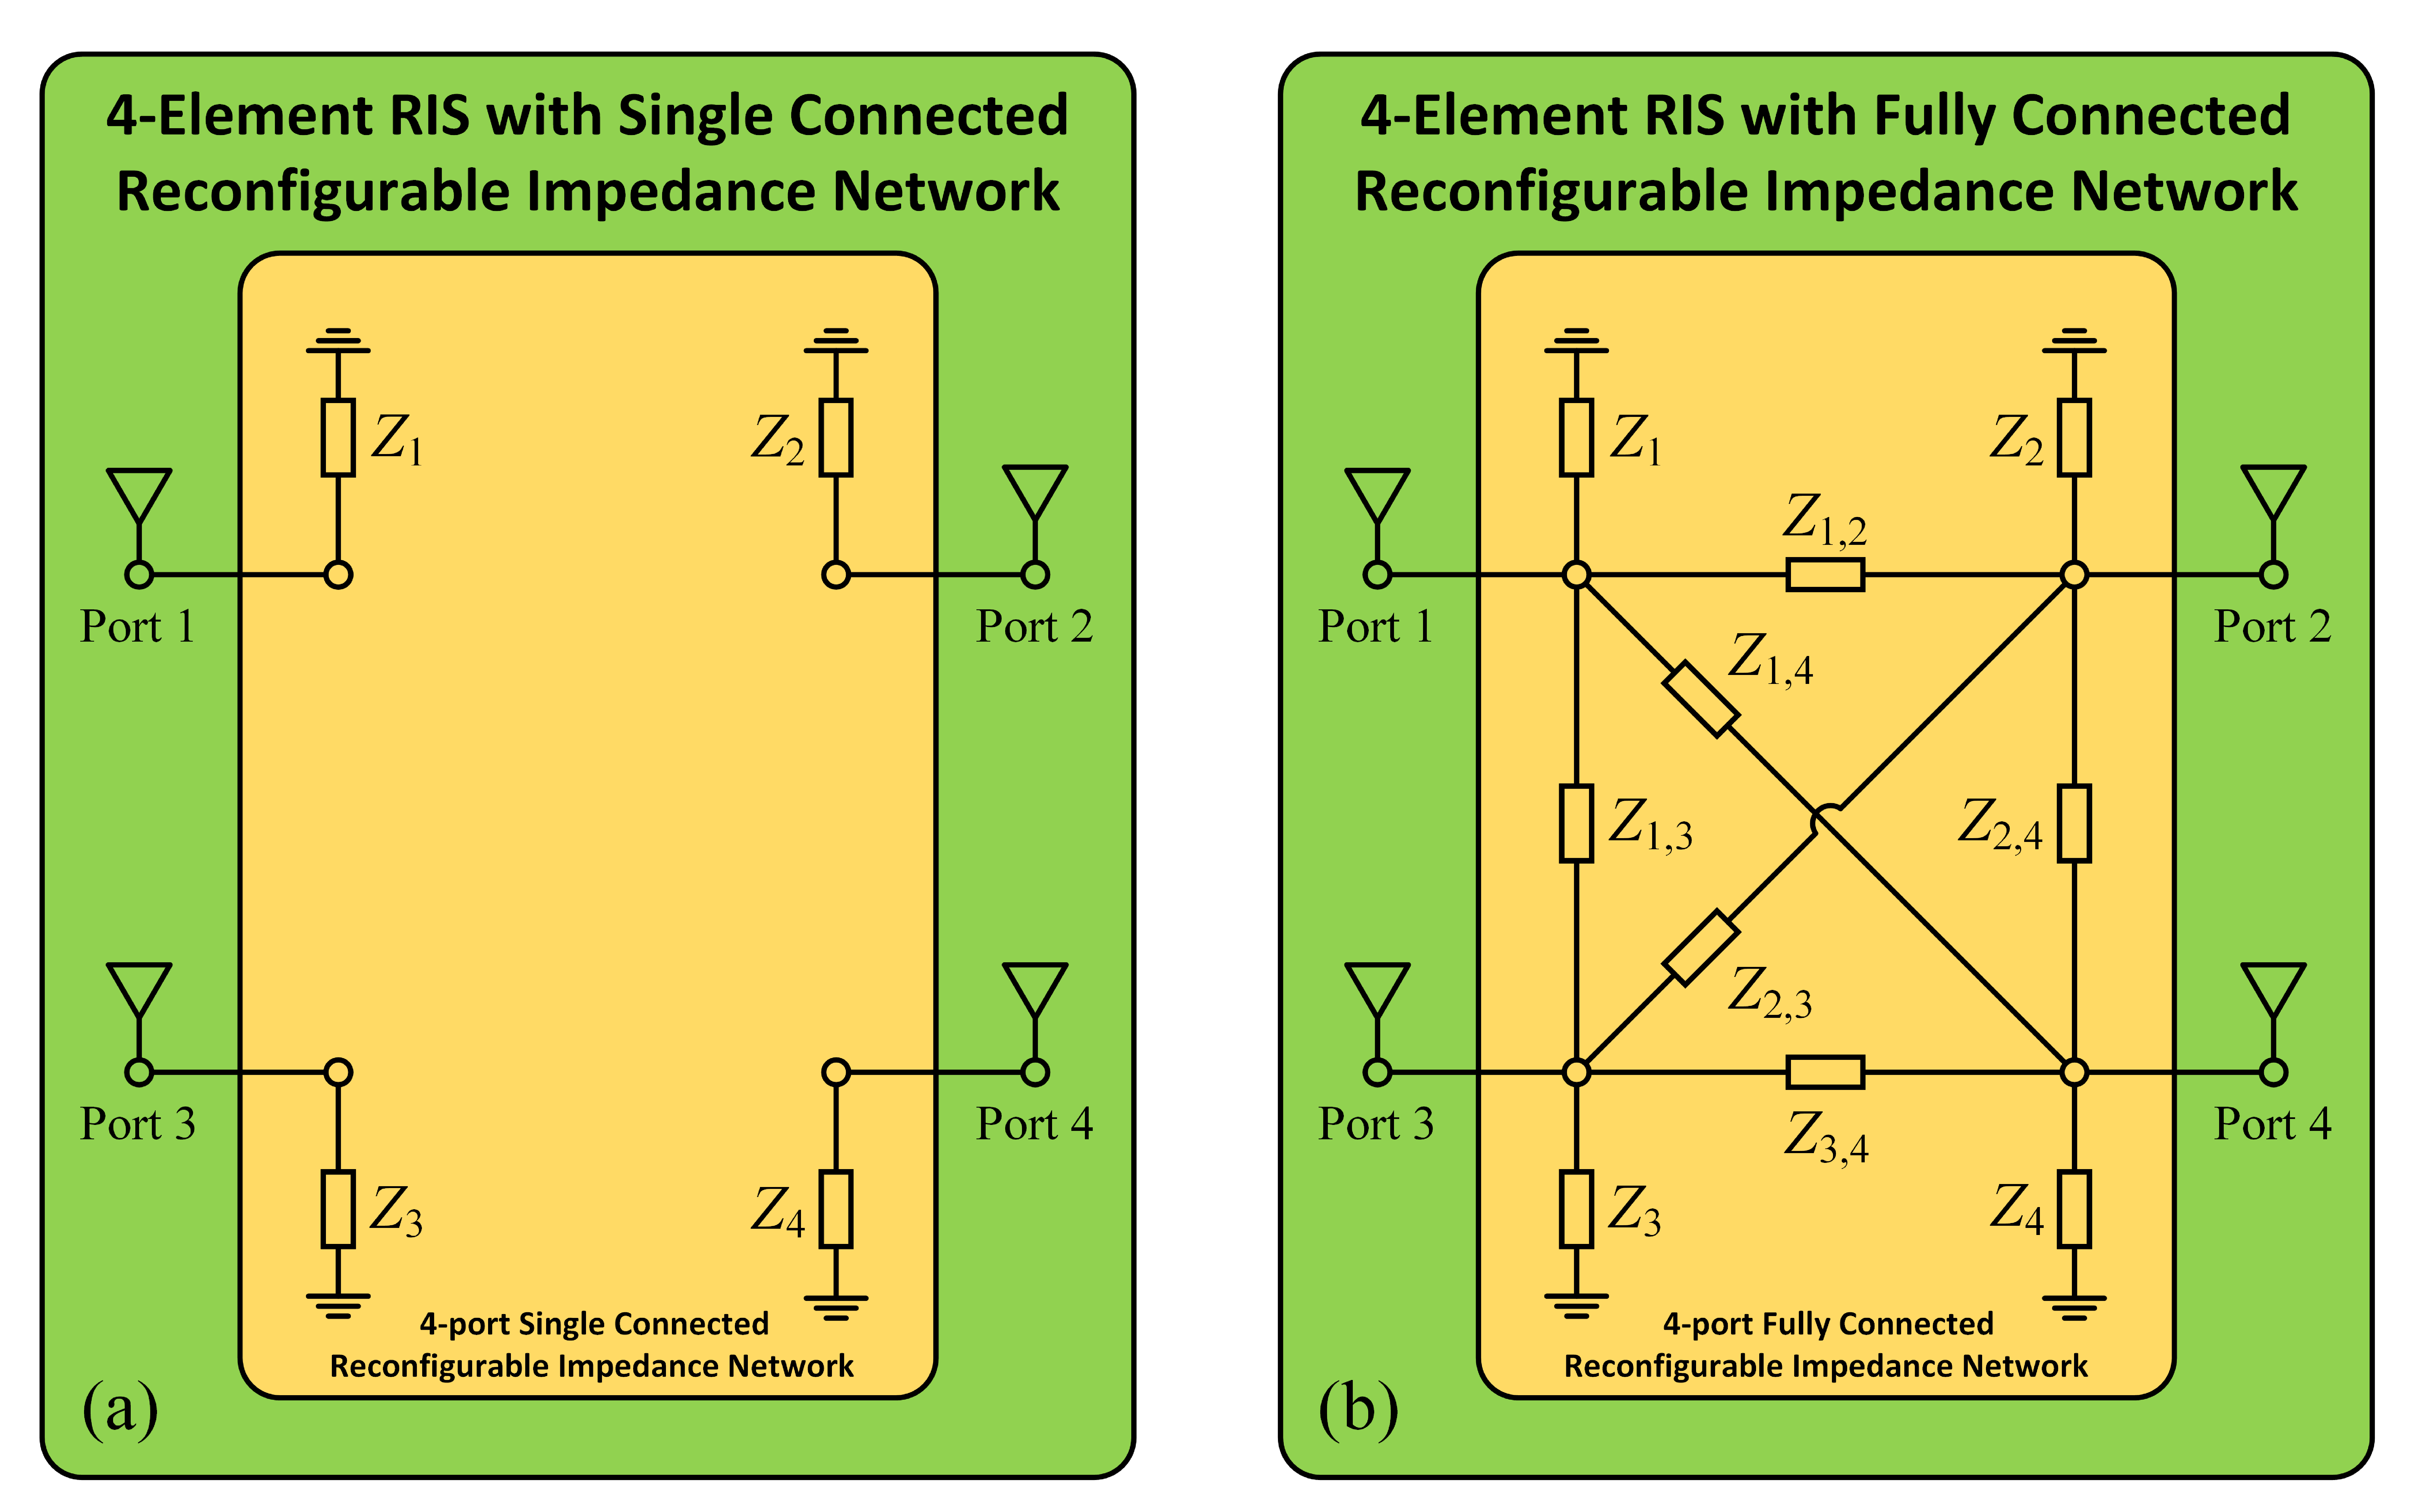
\includegraphics{assets/chapter_2/bd_ris_architecture_1.eps}
				}
				\caption{Network model of a 4-element \gls{ris} with (a) independent scattering and (b) fully cooperative scattering with all elements interconnected. The figure is from \cite{Shen2020a}.}
				\label{fg:bd_ris_architecture_1}
			\end{figure}
			\begin{figure}[H]
				\centering
				\resizebox{0.75\columnwidth}{!}{
					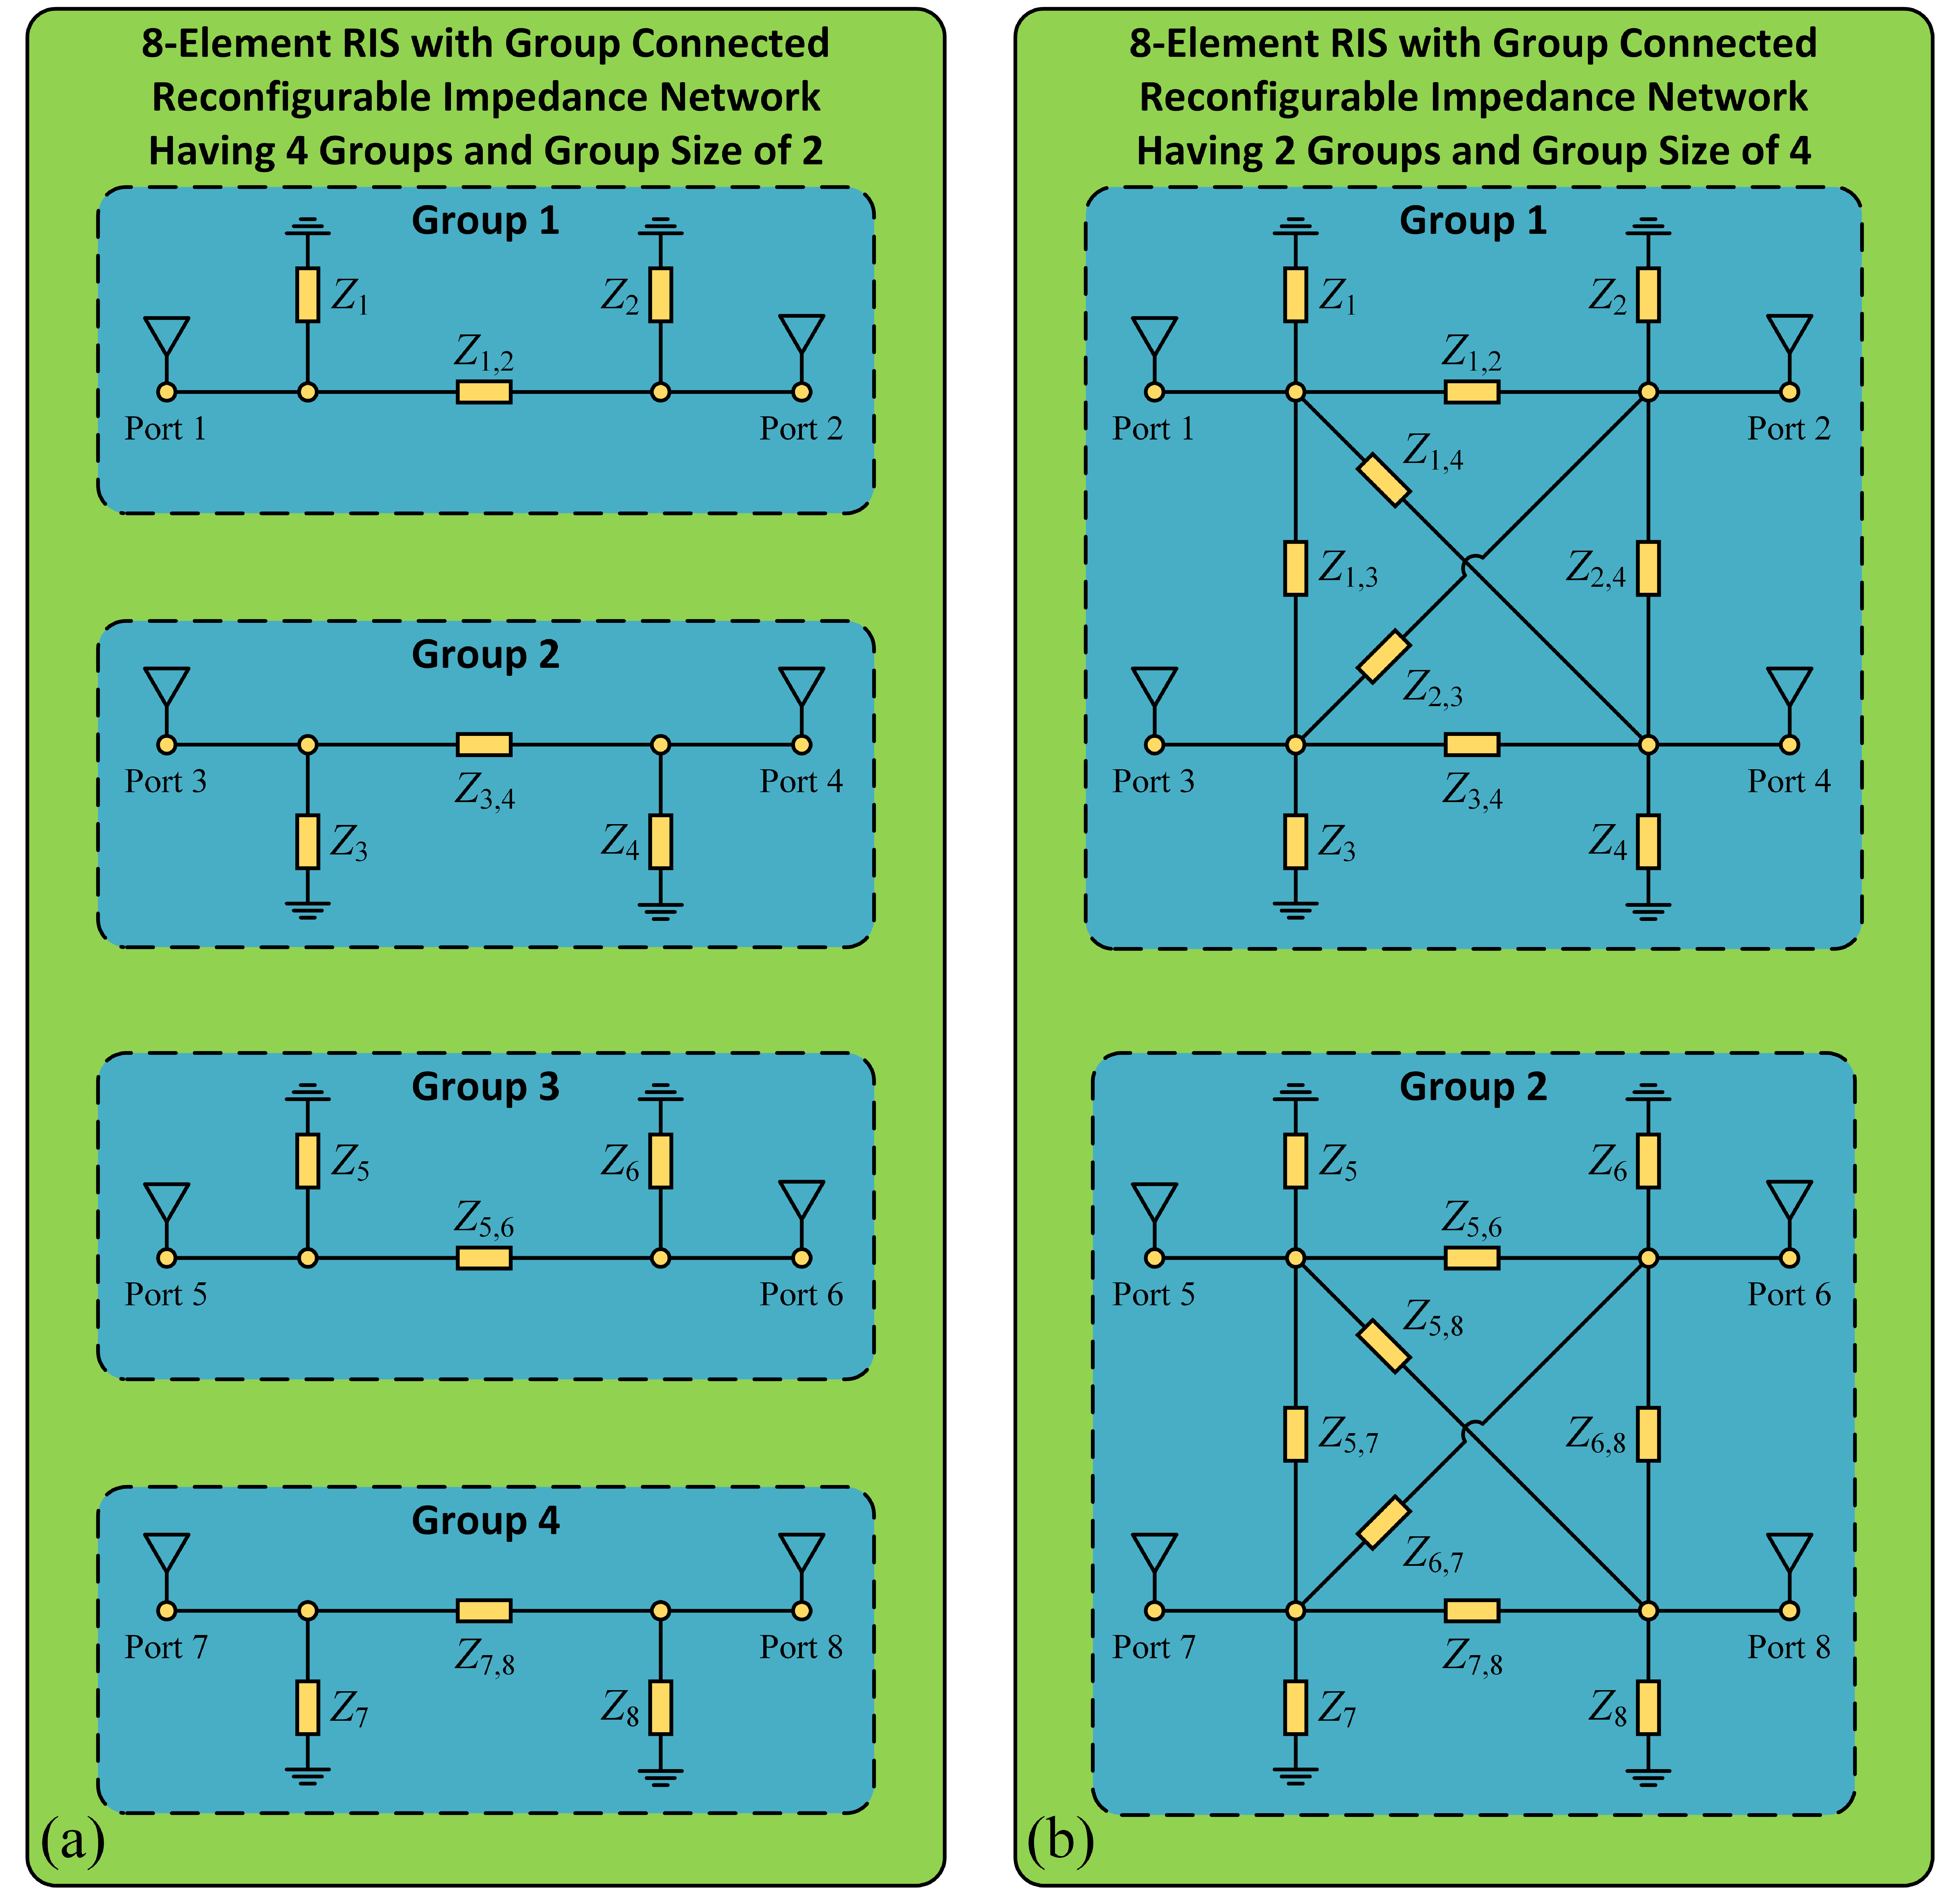
\includegraphics{assets/chapter_2/bd_ris_architecture_2.eps}
				}
				\caption{Network model of an 8-element \gls{ris} with group-wise cooperative scattering of group size (a) 2 and (b) 4. The group size is a design parameter to balance the circuit complexity and scattering performance. The figure is from \cite{Shen2020a}.}
				\label{fg:bd_ris_architecture_2}
			\end{figure}

			A general \gls{bd}-\gls{ris} can be modeled as an $N_\mathrm{S}$-port network that divides into $G$ individual groups, each containing $L \triangleq N_\mathrm{S} / G$ elements interconnected by real-time reconfigurable connections.
			With symmetric components (e.g., capacitors and inductors), the scattering matrix of group $g \in \mathcal{G} \triangleq \{1, \ldots, G\}$ is \cite{Shen2020a}
			\begin{equation}
				\mathbf{\Theta}_g = (\jmath \mathbf{X}_g + Z_0 \mathbf{I})^{-1} (\jmath \mathbf{X}_g - Z_0 \mathbf{I}),
			\end{equation}
			which satisfies both \emph{symmetric} and \emph{unitary} properties
			\begin{subequations}
				\begin{equation}
					\mathbf{\Theta}_g = \mathbf{\Theta}_g^\mathsf{T},
					\label{eq:symmetric_property}
				\end{equation}
				\begin{equation}
					\mathbf{\Theta}_g^\mathsf{H} \mathbf{\Theta}_g = \mathbf{I}.
					\label{eq:unitary_property}
				\end{equation}
			\end{subequations}
			On the other hand, lossless networks may also be built over asymmetric passive components (e.g., ring hybrids and branch-line hybrids) \cite{Ahn2006} such that the symmetric constraint \eqref{eq:symmetric_property} can be relaxed.
			This corresponds to the ultimate passive model where energy conservation \eqref{eq:unitary_property} is the only constraint for each group, as widely considered in quantum physics.
			The overall scattering matrix of asymmetric \gls{bd}-\gls{ris} is thus \emph{block-diagonal with unitary blocks}
			\begin{equation}
				\mathbf{\Theta} = \mathrm{diag}(\mathbf{\Theta}_1,\ldots,\mathbf{\Theta}_G) =
				\begin{bmatrix}
					\mathbf{\Theta}_1 & \mathbf{0} & \cdots & \mathbf{0} \\
					\mathbf{0} & \mathbf{\Theta}_2 & \cdots & \mathbf{0} \\
					\vdots & \vdots & \ddots & \vdots \\
					\mathbf{0} & \mathbf{0} & \cdots & \mathbf{\Theta}_G
				\end{bmatrix},
				\label{eq:bd_scattering_matrix}
			\end{equation}
			where \eqref{eq:unitary_property} is equivalently denoted as $\mathbf{\Theta}_g \in \mathbb{U}^{L \times L}$.
			The group size $L$ is a design parameter to balance the circuit complexity and scattering performance.
			Diagonal (single-connected) and unitary (fully-connected) \gls{ris} can be viewed as extreme cases with group size $L=1$ and $L=N_\mathrm{S}$, respectively.
			Therefore, the \gls{bd} model \eqref{eq:bd_scattering_matrix} is envisioned to be the next-generation theoretical foundation for passive \gls{ris}, which grants more design freedom and stronger signal processing capability.

			It is also worth mentioning that each group can be abstracted as a mathematical graph with $L$ vertices and a variable number of edges \cite{Nerini2023a}.
			One element is in the same group with another if and only if there is at least one path (via edges) between them.
			It implies that instead of connecting every pair of elements, the practical circuit can be designed to have a sparse graph with only a few connections, which is beneficial for reducing the circuit complexity and power loss from non-ideal components.
			Antenna directivity and radiation pattern should also be modelled in the scattering matrix, especially when the locations of users or \gls{ris} are not fixed.
			This has motivated the concept of \gls{star}-\gls{ris} \cite{Mu2021,Liu2021} and multi-sector \gls{ris} \cite{Li2023c} where incident wave is partially steered to various directions for different users.
		\end{subsubsection}
	\end{subsection}
\end{section}

\begin{section}{\glsfmtfull{wpt}}
	\begin{subsection}{Introduction}
		Wireless devices are becoming smarter as well as more energy-efficient and eco-friendly.
		Koomey's law \citep{Koomey2011} predicts the computing efficiency roughly doubles every 19 months and the amount of power needed for the same operation decreases to 1\% in a decade.
		Over the past 15 years, the rise of low-power technologies like \gls{wsn} and \gls{iot} have hatched life-changing applications including smart homes, digital healthcare, and industrial automation.
		% This low-power trend has been accelerated by the rise of \gls{iot} and \gls{wsn} technologies, which enabled revolutionary applications including smart homes, digital healthcare, and industrial automation.
		Today, \gls{rfid} tags and basic sensors (e.g., thermometer and proximeter) can operate on microwatts of power \cite{Huang2019,Hao2018}, while communication protocols like \gls{ble} and \gls{lorawan} only consume tens of milliwatts \cite{Correia2017b}.
		This low-power trend together with the upsurge of mobile devices is calling for a \emph{truly wireless} energy solution that eliminates the need for periodic cable plugging or battery replacement.
		% While solutions like solar and piezoelectric offer benefits in specific scenarios, their bulky components, unpredictable power sources, and limited range make them unsuitable for most wireless applications.
		While great successes have been witnessed for candidates like solar and piezoelectric, their prospects in wireless systems remain unclear due to the bulky converter, unpredictable source, and limited operation range.
		One promising solution on the horizon is \gls{wpt} through electromagnetic waves.
		It can be classified into two categories based on the operation principle \cite{Zhou2022}:
		\begin{itemize}
			\item \emph{Non-radiative near-field:} Power is transferred over a short distance (typically a few centimeters) by inductive coupling between coils or capacitive coupling between electrodes in a field-to-field manner. The former has been widely standardized (e.g., Qi 2.0) and commercialized (e.g., wireless charging pads), while the latter is still in the research stage.
			\item \emph{Radiative far-field:} Power is transferred over a long distance (typically a few meters) by directional microwave or laser beams between antennas in a point-to-point manner. It shares many similarities with \gls{rf} communication (e.g., infrastructure and wireless environment) but suffers from lower energy efficiency than non-radiative \gls{wpt} due to pathloss.
		\end{itemize}

		Radiative \gls{wpt}\footnote{In the following part of the thesis, \gls{wpt} refers to radiative \gls{wpt}.} brings numerous opportunities to future wireless networks.
		First, it completely eliminates wired connections and can be integrated into existing wireless systems with minimum modifications.
		Those properties translate to simple deployment, high scalability, and low maintenance cost.
		Second, the power can be simultaneously radiated to multiple devices on demand in a predictable, sustainable and reliable manner.
		This supports our initial vision and is different from other uncontrollable and intermittent energy sources.
		Third and most importantly, radio waves carries power and information simultaneously.
		\gls{wpt} can therefore be jointly designed with \gls{wit} to make the most of radiation, spectrum and infrastructures.
		However, energy efficiency and safety concerns have been two major obstacles that limit the practical development of \gls{wpt}.
		In Section \ref{sc:swipt}, we will discuss how \gls{ris} can help address these issues.
	\end{subsection}

	\begin{subsection}{Modules and Coupling Effect}
		\begin{figure}[H]
			\centering
			\resizebox{\columnwidth}{!}{
				\begin{circuitikz}[transform shape,align=center,font=\footnotesize]
	\draw(0,0) node[draw](rf){\gls{rf}\\source};
	\draw(rf.east) node[txantenna]{};
	\draw(1,1) node{Tx};
	\draw(4.875,2) node[draw]{\gls{ris}};
	\draw(4.875,1) node[draw]{Channel};
	\draw(10,0) node[draw](mc){Matching\\network};
	\draw(mc.west) node[rxantenna,xscale=-1]{};
	\draw(8.7,1) node{Rx};
	\draw(mc.east) to ++(0.85,0) node[anchor=west,draw](d){Diode};
	\draw(d.east) to ++(0.85,0) node[anchor=west,draw](lpf){Low-pass\\filter};
	\draw(lpf.east) to ++(1,0) node[anchor=west,draw](dd){\gls{dc}-\gls{dc}\\converter};
	\draw(dd.east) to ++(1,0) node[anchor=west,draw](s){Storage};

	\draw [dashed] (-0.95,-0.75) rectangle (3.75,2.75);
	\draw (1.4,3) node[]{Energy transmitter};
	\draw [dotted] (6.25,-0.5) rectangle (15.6,2.5);
	\draw (10.925,2) node[]{Rectenna};
	\draw [dotted] (16,-0.5) rectangle (20.5,1.25);
	\draw (18.25,0.875) node[]{Power management unit};
	\draw [dashed] (6,-0.75) rectangle (20.75,2.75);
	\draw (13.375,3) node[]{Energy receiver};

	\draw (-0.95,-1) node[]{$P_{\mathrm{DC}}^{\mathrm{T}}$};
	\draw (3.75,-1) node[]{$P_{\mathrm{RF}}^{\mathrm{T}}$};
	\draw (6,-1) node[]{$P_{\mathrm{RF}}^{\mathrm{R}}$};
	\draw (15.8,-1) node[]{$P_{\mathrm{DC}}^{\mathrm{R}}$};
	\draw (20.5,-1) node[]{$P_{\mathrm{DC}}^{\mathrm{S}}$};

	\draw[gray,dashdotted,-latex] (10.925,-0.5) to ++(0,-1.5) to ++(-1,0) node[anchor=east,draw](c){Channel\\feedback};
	\draw[gray,dashdotted,latex-] (1.4,-0.75) to ++(0,-1.25) to ++(1,0) node[anchor=west,draw](s){Signal\\optimization};
	\draw[gray,dashdotted,-latex] (c.west) to (s.east);
	\draw[gray] (6.45,-2) node[]{Reverse\\communication link};
\end{circuitikz}

			}
			\caption{Block diagram of a closed-loop \gls{ris}-aided \gls{wpt}.}
			\label{fg:wpt_architecture}
		\end{figure}

		The block diagram a closed-loop \gls{ris}-aided \gls{wpt} system is illustrated in Fig. \ref{fg:wpt_architecture}.
		The \gls{rf} signal is generated and radiated by the energy transmitter, propagated through a wireless channel in the presence of a \gls{ris}, captured by the antenna(s) at the receiver, converted to \gls{dc} power by rectifier(s), then passed to the power management unit.
		Upon successful harvesting, the \gls{dc} power is either delivered directly to the device or stored in a battery/super capacitor for future operations.
		When a feedback link is available, one can acquire \gls{csi} at the energy transmitter and exploit it for signal optimization.
		Such a closed-loop \gls{ris}-aided \gls{wpt} system can provide a complete control of transmitter, channel, and receiver, which is essential for maximizing the end-to-end power transfer efficiency
		\begin{equation}
			\eta = \frac{P_{\mathrm{DC}}^\mathrm{S}}{P_{\mathrm{DC}}^\mathrm{T}} = \underbrace{\frac{P_{\mathrm{RF}}^\mathrm{T}}{P_{\mathrm{DC}}^\mathrm{T}}}_{\eta_1} \underbrace{\frac{P_{\mathrm{RF}}^\mathrm{R}}{P_{\mathrm{RF}}^\mathrm{T}}}_{\eta_2} \underbrace{\frac{P_{\mathrm{DC}}^\mathrm{R}}{P_{\mathrm{RF}}^\mathrm{R}}}_{\eta_3} \underbrace{\frac{P_{\mathrm{DC}}^\mathrm{S}}{P_{\mathrm{DC}}^\mathrm{R}}}_{\eta_4},
		\end{equation}
		where $P_{\mathrm{DC}}^\mathrm{T}$ is the transmitted \gls{dc} power, $P_{\mathrm{RF}}^\mathrm{T}$ is the transmitted \gls{rf} power, $P_{\mathrm{RF}}^\mathrm{R}$ is the received \gls{rf} power, $P_{\mathrm{DC}}^\mathrm{R}$ is the received \gls{dc} power, and $P_{\mathrm{DC}}^\mathrm{S}$ is the stored \gls{dc} power.
		The power conversion efficiencies are specified below:
		\begin{itemize}
			\item $\eta_1$: Transmitter \gls{dc}-to-\gls{rf} conversion efficiency\footnote{This is different from \gls{pae} used in amplifier rating, which takes into account both \gls{dc} power and input waveform power \cite{Joung2015}.} that depends on the \gls{rf} power amplifier and transmit antenna. It is also called ``drain efficiency'' and state-of-the-art designs can achieve $\eta_1 \ge 70\%$ \cite{Alizadeh2020}.
			\item $\eta_2$: Channel \gls{rf}-to-\gls{rf} conversion efficiency that depends on the wireless environment and \gls{ris} configuration. This is the major bottleneck of \gls{wpt} since the radiated power is inversely proportional to the propagation distance squared.
			\item $\eta_3$: Receiver \gls{rf}-to-\gls{dc} conversion efficiency that depends on the impedance matching and rectifier design. We will discuss its behavior and modelling in the next subsection.
			\item $\eta_4$: Storage \gls{dc}-to-\gls{dc} conversion efficiency that depends on the converter circuit and battery characteristics. Modern power management units can achieve a charging efficiency $\eta_4 \ge 90\%$ \cite{Tan2012}.
		\end{itemize}
		It is worth mentioning that $\eta_1$ and $\eta_3$ also depend on the characteristics of input waveform like power level, carrier frequency, and \gls{papr} \cite{Clerckx2016a}.
		Extensive efforts have been contributed from \gls{rf}, wireless communications, and power electronic communities to improve the conversion efficiency of individual modules.
		However, it is often overlooked in the literature that a practical \gls{wpt} system is highly \emph{non-linear} since the amplifier and rectifier are very sensitive to the input waveform.
		This non-linear behavior can lead to a \emph{coupling effect} between the modules, such that optimizing $\eta_1$ to $\eta_4$ independently does not necessarily maximize the end-to-end power efficiency $\eta$ \cite{Clerckx2016a}.
		Besides, the system modeling and analysis are subject to practical constraints like diode threshold and reverse-breakdown voltages, device parasitics, impedance mismatch, and harmonic generation  \citep{Valenta2014}.
	\end{subsection}

	\begin{subsection}{Non-Linear Harvester Behavior}
		\begin{subsubsection}{Equivalent Circuits}
			\begin{figure}[H]
				\centering
				\subfloat[Rectenna]{
					\resizebox{0.45\columnwidth}{!}{
						\begin{circuitikz}[transform shape]
	\draw (0,0) to [sV=$v_{\mathrm{S}}$] (0,2);
	\draw (0,2) to [short] (1,2);
	\draw (1,2) to [generic,l=$Z_{\mathrm{A}}$] (3,2);
	\draw (3,2) to [short] (4,2);
	\draw (4,2) to [generic,l=$Z_{\mathrm{in}}$, v<=$v_{\mathrm{in}}$] (4,0);
	\draw (4,0) to [short] (2,0) node[ground](GND){};
	\draw (2,0) to [short] (0,0);
\end{circuitikz}

					}
					\label{fg:rectenna}
				}
				\subfloat[Half-wave rectifier]{
					\resizebox{0.45\columnwidth}{!}{
						\begin{circuitikz}[transform shape]
	\draw (0,0) to [sV=$v_{\mathrm{in}}$] (0,2);
	\draw (0,2) to [short] (0.25,2);
	\draw (0.25,2) to [D, v<=$v_{\mathrm{D}}$] (2.25,2);
	\draw (2.25,2) to [short, -*] (2.5,2);
	\draw (2.5,2) to [C, l_=$C$, -*] (2.5,0);
	\draw (2.5,2) to [short] (4.25,2);
	\draw (4.25,2) to [R=$R_{\mathrm{L}}$, v=$v_{\mathrm{out}}$] (4.25,0);
	\draw (4.25,0) to [short] (2,0) node[ground](GND){};
	\draw (2,0) to [short] (0,0);
\end{circuitikz}

					}
					\label{fg:halfwave_rectifier}
				}
				\caption{
					Equivalent circuit of (a) rectenna and (b) single-diode half-wave rectifier.
				}
				\label{fg:harvester_circuit}
			\end{figure}
			The rectifier is a nonlinear circuit that converts the \gls{rf} signal to \gls{dc} power by rectifying and filtering the input signal.
			Figs. \ref{fg:harvester_circuit} illustrates the equivalent circuits of a rectenna (antenna and rectifier) and a single-diode half-wave rectifier, where $v_{\mathrm{S}}$ is the source voltage on the receive antenna, $Z_{\mathrm{A}} = R_{\mathrm{A}} + \jmath X_{\mathrm{A}}$ is the antenna impedance, $Z_{\mathrm{in}} = R_{\mathrm{in}} + \jmath X_{\mathrm{in}}$ is the total impedance of the matching network and rectifier, $v_{\mathrm{in}}$ is input voltage on the matching network and rectifier, $v_{\mathrm{D}}$ is the diode voltage, $C$ is the buffer capacitance, $R_{\mathrm{L}}$ is the rectifier load resistance, and $v_{\mathrm{out}}$ is the output voltage.
			It is worth mentioning that the half-wave rectifier is the most popular choice in \gls{wpt} literature due to its simple behavior and low cost.
			Other rectifier topologies like full-wave, bridge, and voltage doubler can potentially improve the \gls{rf}-to-\gls{dc} conversion efficiency \cite{Rotenberg2020}, but their modeling and analysis are much more complicated.
		\end{subsubsection}

		\begin{subsubsection}{Operation Regions and Signal Models}
			The diode is the key non-linear component that determines to the harvested energy.
			Generally speaking, the behavior of any rectenna can be separated into three operation regions \cite{Clerckx2016a}:
			\begin{itemize}
				\item \emph{Linear region:} When the input power level is relatively low, the output power is proportional to the input and the \gls{rf}-to-\gls{dc} conversion efficiency $\eta_3$ is a constant. Most early \gls{wpt} research (especially from communications society) assume the rectenna works in this region. For a received signal $y(t)$, the harvested \gls{dc} power in this region can be modelled as
				\begin{equation}
					P_\mathrm{DC}^\mathrm{R} = \eta_3 P_\mathrm{RF}^\mathrm{R} = \eta_3 \mathbb{E}\bigl\{ \lvert y(t) \rvert^2 \bigr\},
					\label{eq:dc_power_linear}
				\end{equation}
				which suggests that maximizing the received \gls{rf} signal power is sufficient to maximize the harvested \gls{dc} power.
				\item \emph{Non-linear (transition) region:} When the input power level is moderate, the output power increases \emph{exponentially} with the input and $\eta_3$ is significantly higher than the linear region. This is the most interesting region that can be exploited to improve the overall power efficiency.
				For a tractable model, consider a perfectly matched ($Z_\mathrm{in} = Z_\mathrm{A}^*$) half-wave rectifier in Fig.~\subref*{fg:halfwave_rectifier} and assume the voltage across the matching network is negligible. The received \gls{rf} power is totally transferred to the rectifier input $P_\mathrm{RF}^\mathrm{R} = \mathbb{E}\bigl\{ \lvert y(t) \rvert^2 \bigr\} = \mathbb{E}\bigl\{ \lvert v_\mathrm{in}(t) \rvert^2 / R_\mathrm{in} \bigr\} = \mathbb{E}\bigl\{ \lvert v_\mathrm{in}(t) \rvert^2 / R_\mathrm{A} \bigr\}$ such that the voltage sources can be expressed in terms of the received signal \cite{Clerckx2016a}
				\begin{equation}
					v_\mathrm{in}(t) = y(t) \sqrt{R_\mathrm{A}}, \quad v_\mathrm{S}(t) = 2 y(t) \sqrt{R_\mathrm{A}}.
				\end{equation}
				The current passing through the diode is given by the characteristic equation $i_\mathrm{D}(t) = I_\mathrm{S} \bigl( \exp(v_\mathrm{D}(t) / n v_\mathrm{T}) - 1 \bigr)$, where $I_\mathrm{S}$ is the reverse bias saturation current, $v_\mathrm{T}$ is the thermal voltage, and $n$ is the ideality factor. Its Taylor expansion around the steady point $-v_\mathrm{out}$ is \cite{Clerckx2016a}
				\begin{equation}
					i_\mathrm{D}(t) = \sum_{i=0}^\infty k_i \bigl(v_\mathrm{D}(t)+v_\mathrm{out}\bigr)^i = \sum_{i=0}^\infty k_i v_\mathrm{in}^i(t) = \sum_{i=0}^\infty k_i R_\mathrm{A}^{i/2} y^i(t),
				\end{equation}
				where $k_0 = I_\mathrm{S} \bigl(\exp(-{v_\mathrm{out}}/{n v_\mathrm{T}})-1\bigr)$, $k_i = I_\mathrm{S} \frac{\exp(-v_\mathrm{out}/n v_\mathrm{T})}{i!(n v_\mathrm{T})^i}$ for $k \in \mathbb{N}$.
				The rectifier output \gls{dc} current can be written as a function of the received signal
				\begin{equation}
					i_\mathrm{out} = \sum_{i=0}^\infty k_i R_\mathrm{A}^{i/2} \mathbb{E}\bigl\{ y^i(t) \bigr\} = \sum_{i=0,\text{even}}^\infty k_i R_\mathrm{A}^{i/2} \mathbb{E}\bigl\{ y^i(t) \bigr\}
					\label{eq:dc_current_expansion}
				\end{equation}
				where the second equality is because $\mathbb{E}\bigl\{y^i(t)\bigr\} = 0$ for odd $i$. Note that the dependency of $k_i$ on $-v_\mathrm{out}=-i_\mathrm{out} R_\mathrm{L}$ makes it nontrivial to formulate a closed-form expression for the harvested \gls{dc} power.
				Fortunately, it is shown in \cite{Clerckx2016a} that maximizing the harvested \gls{dc} power is equivalent to maximizing the quantity
				\begin{equation}
					z \triangleq \sum_{i=2,\text{even}}^\infty \beta_i \mathbb{E}\bigl\{ y^i(t) \bigr\},
					\label{eq:dc_power_nonlinear}
				\end{equation}
				where $\beta_i = I_\mathrm{S} \frac{R_\mathrm{A}^{i/2}}{i!(n v_\mathrm{T})^i}$ is a constant. Truncating \eqref{eq:dc_power_nonlinear} at the second order yields the same result as \eqref{eq:dc_power_linear}, which suggests that the linear model is a special case of the more accurate non-linear model. For a moderate excitation, the contribution of higher-order terms is significant and should be modelled in the harvested \gls{dc} power.
				\item \emph{Saturation region:} When the input power level is too high, the diode works in the reverse breakdown region, the rectifier is saturated, and the output power is a constant. This is the region where the $\eta_3$ significantly drops and should be avoided by circuit design.
				For a fixed rectenna with Gaussian input signal, a parametric model was proposed in \cite{Boshkovska2015}
				\begin{equation}
					P_{\mathrm{DC}}^\mathrm{R} = \frac{\Psi_{\mathrm{DC}}-P_{\text{sat}}\Omega}{1-\Omega}, \quad \Psi_{\mathrm{DC}} = \frac{P_{\text{sat}}}{1+\exp\bigl(-a(P_{\mathrm{RF}}^\mathrm{R}-b)\bigr)}, \quad \Omega = \frac{1}{1 + \exp(ab)},
					\label{eq:saturation_model}
				\end{equation}
				where the constant $P_{\text{sat}}$ denotes the maximum harvested power when the rectifier is saturated, and the constants $a$ and $b$ model the nonlinear charging rate with respect to input power and the minimum turn-on voltage of the rectifier, respectively.
				Parameters $P_{\text{sat}}$, $a$, and $b$ can be obtained by curve fitting over measurement results.
			\end{itemize}

			The exact boundaries between those regions depend on the rectifier circuit and input waveform \citep{Zeng2017}.
			Signals with a higher \gls{papr} usually exhibit the nonlinear and saturation effects at lower input power levels.
			For example, the nonlinear region is typically $[-20,0]$ dBm for a \gls{cw} and $[-30,-10]$ dBm for a multisine \citep{DelPrete2016}.
			This not only motivates adaptive multi-carrier waveform designs \cite{Clerckx2016a,Zeng2017,Huang2017,Shen2021} but also calls for a joint optimization of the transmitter, channel (via \gls{ris}), and receiver to improve the end-to-end power efficiency.
		\end{subsubsection}
	\end{subsection}
\end{section}

\begin{section}{\glsfmtfull{swipt}}\label{sc:swipt}
	\begin{subsection}{Introduction}
		\gls{wit} and \gls{wpt} have been treated separately over the past century and have made significant progress in their respective fields.
		Interestingly, electromagnetic waves carry information and energy simultaneously and the same signal can be used for communication and power transfer.
		The idea of \gls{swipt} was first proposed in 2008 \cite{Varshney2008} and has since attracted significant attention from both academia and industry.
		It is a promising solution to connect and energize trillions of low-power mobile devices, providing power at microwatt level and coverage up to tens of meters in a unified manner \cite{Clerckx2018b}.
		\gls{swipt} can also smoothly shift between the two extreme cases to fully exploit the \gls{rf} spectrum and network infrastructure.
		It is envisioned that future network providers will be able to offer a complete wireless solution including data and power services, which is essential for the upcoming intelligent era.

		One of the most important issues in \gls{swipt} is that the energy harvester requires a much higher received signal power (several orders of magnitude) than the information decoder \cite{Clerckx2019}.
		Since the channel \gls{rf}-to-\gls{rf} efficiency $\eta_2$ is the primary constraint on the overall power efficiency, how to combat the pathloss and fading effects has been recognized as a crucial research topic for \gls{wpt} \gls{swipt}.
		Fortunately, this issue can be effectively mitigated by introducing a \gls{ris} to the environment.
		By carefully tuning the scatter response of the \gls{ris} elements, one can potentially achieve the following benefits:
		\begin{itemize}
			\item \emph{Energy focusing:} The scattered waves can be steered towards the receivers or focused on a dedicated ``hotspot zone'' to increase the harvester input power level. This is also helpful to extend the coverage and improve the reliability of the energy link.
			\item \emph{Beam splitting:} Instead of transmitting one strong beam towards each user, the energy signal can be split into multiple weaker beams rerouted by the \gls{ris} to even out the spatial power distribution. This is useful to bypass physical obstacles (especially in high-frequency and large-scale networks) and reduce the health risk of radiation.
		\end{itemize}
		\gls{ris} can also be used to assist the information link by \gls{snr} enhancement and interference suppression, as mentioned in subsection \ref{sc:ris_applications}.
	\end{subsection}

	\begin{subsection}{\glsfmtfull{r-e} Tradeoff}
		Despite \gls{wit} and \gls{wpt} share many similarities, their difference in design objectives, system architectures, and practical constraints make a joint implementation of \gls{swipt} particularly challenging.
		Some preference of \gls{wit} and \gls{wpt} are inherently conflicting, for example:
		\begin{itemize}
			\item \emph{Waveform and modulation:} Under an average power constraint, \gls{wit} favors Gaussian signaling with maximum entropy distribution \cite{Cover2005} while \gls{wpt} prefers deterministic (unmodulated) multisine with higher \gls{papr} \cite{Trotter2009}.
			\item \emph{Channel:} In a \gls{mimo} scenario, \gls{wit} favors full-rank \gls{nlos} with high spatial diversity while \gls{wpt} prefers rank-deficient \gls{los} with high spatial correlation \cite{Wu2022a}.
			\item \emph{Receiver:} The power sensitivity is usually in the range of -40 to -80 dBm for information receivers and -10 to -30 dBm for energy harvesters \cite{Lu2015}.
		\end{itemize}
		Those disparities translate to a fundamental tradeoff between information and power transfer in \gls{swipt} systems, which is often quantified by a convex \emph{\gls{r-e} region}.
		\begin{equation}
			\mathcal{C}_\mathrm{R-E}(P) \triangleq \Bigl\{ (r,e) : 0 \le r \le \log(1 + \gamma), \ 0 \le e \le z \Bigr\},
		\end{equation}
		where $P$ is the average transmit power, $\gamma$ is the \gls{snr} at the information decoder, and $z$ defined in \eqref{eq:dc_power_nonlinear} is uniquely mapped to the harvested \gls{dc} power.
		Each point in this region corresponds to a \emph{rate-energy pair} achieved by a particular \emph{resource allocation scheme}.
		It is worth mentioning that different transceive strategies (e.g., waveform and receiver design) can lead to totally different \gls{r-e} regions (instead of different points in the same region), which motivates a joint optimization of the transmitter, channel, and receiver.
	\end{subsection}

	\begin{subsection}{System Architecture}

		\begin{subsubsection}{Information and Energy Flows}

		\end{subsubsection}

		\begin{subsubsection}{Receiver Architectures}

		\end{subsubsection}
		As shown in Figs. \subref*{fg:swipt_colocated} and \subref*{fg:swipt_separated}, \gls{swipt} can be classified into two categories based on the receiver configuration:
		% \begin{itemize}
		% 	\item \emph{\gls{swipt}:} Energy and information are simultaneously delivered in the downlink to co-located and/or separated information receiver(s) and energy receiver(s);
		% 	\item \emph{\gls{wpcn}:} Energy is delivered in the downlink to active device(s) that generate and transmit information-bearing signals in the uplink;
		% 	\item \emph{\gls{wpbc}:} Energy is delivered in the downlink to passive node(s) that reflect part of incoming waves and embed information in the uplink.
		% \end{itemize}
		\begin{figure}[H]
			\centering
			\subfloat[\gls{swipt} with co-located receiver]{
				\resizebox{7cm}{!}{
					\begin{tikzpicture}[align=center,thick]
	\draw (0,0) node[draw,minimum width=2cm](t){ET+{\color{blue}IT}};
	\draw[-latex](t.east) -- ++(2.5,0) node[draw,solid,anchor=west,minimum width=2cm](r){ER+{\color{blue}IR}};
	\draw[-latex,blue,decorate,decoration=snake] (t.east) -- (r);
\end{tikzpicture}

				}
				\label{fg:swipt_colocated}
			}
			\subfloat[\gls{swipt} with separated receivers]{
				\resizebox{7cm}{!}{
					\begin{tikzpicture}[align=center,thick]
	\draw (0,0) node[draw,minimum width=2cm](t){ET+{\color{blue}IT}};
	\draw[-latex](t.east) -- (4,0.5) node[draw,solid,anchor=west,minimum width=1cm]{ER};
	\draw[-latex,blue,decorate,decoration=snake](t.east) -- (4,-0.5) node[draw,solid,anchor=west,minimum width=1cm]{IR};
\end{tikzpicture}

				}
				\label{fg:swipt_separated}
			}
			\\
			\subfloat[Monostatic backscatter]{
				\resizebox{7cm}{!}{
					\begin{tikzpicture}[align=center,thick]
	\draw (0,0) node[draw,minimum width=2cm](t){ET+{\color{blue}IR}};
	\draw[-latex](t.north east) -- ++(2.5,0) node[draw,solid,anchor=north west,minimum width=2cm](r){ER+{\color{blue}IT}};
	\draw[-latex,blue,decorate,decoration=snake](r.south west) -- (t.south east);
\end{tikzpicture}

				}
				\label{fg:backcom_monostatic}
			}
			\subfloat[Bistatic backscatter]{
				\resizebox{7cm}{!}{
					\begin{tikzpicture}[align=center,thick]
	\draw (0,0.5) node[draw,solid,anchor=west,minimum width=1cm](et){ET};
	\draw (0,-0.5) node[draw,blue,solid,anchor=west,minimum width=1cm](ir){IR};
	\draw[-latex](et.east) -- (4,0) node[draw,solid,anchor=west,minimum width=2cm](erit){ER+{\color{blue}IT}};
	\draw[-latex,blue,decorate,decoration=snake] (erit.west) -- (ir.east);
\end{tikzpicture}

				}
				\label{fg:backcom_bistatic}
			}
			\caption{
				Information and energy flows in different WIPT schemes. Dashed and dotted lines denote energy and information flows, respectively.
			}
			\label{fg:wipt_schemes}
		\end{figure}

	\end{subsection}
\end{section}

\begin{section}{\glsfmtfull{bc}}
	\begin{subsection}{\glsfmtfull{mbc}}

	\end{subsection}

	\begin{subsection}{\glsfmtfull{bbc}}

	\end{subsection}

	\begin{subsection}{\glsfmtfull{ambc}}

	\end{subsection}

	\begin{subsection}{\glsfmtfull{sr}}

	\end{subsection}
\end{section}

% \begin{section}{\glsfmtfull{im}}

% \end{section}

\begin{section}{\glsfmtfull{mimo}}
	\begin{subsection}{\glsfmtfull{pc}: Channel Shaping}

	\end{subsection}

	\begin{subsection}{\glsfmtfull{ic}: Interference Alignment}

	\end{subsection}
\end{section}

% %!TEX root = ../thesis.tex

\graphicspath{{assets/chapter_3/}}

\chapter{Getting started}




\begin{section}{Introduction}
	% The quest for reliable, high-speed, and ubiquitous wireless connectivity has been long-standing since Marconi's illuminating radio in 1895.
	% Great successes have been made at transmitter and receiver sides over the past century, and the society is unprecedentedly close to the Shannon limit \cite{Shannon1948}.
	Today we are witnessing a paradigm shift from connectivity to intelligence, where the wireless environment is no longer a chaotic medium but a conscious agent that serves on demand.
	This is empowered by the recent advances in \gls{ris}, a real-time programmable metasurface of numerous non-resonant sub-wavelength scattering elements.
	It can manipulate the amplitude, phase, frequency, and polarization of the scattered waves \cite{Basar2019} with a higher energy efficiency, lower cost, lighter footprint, and greater scalability than relays.
	Using \gls{ris} for {passive beamforming} has attracted significant interest in wireless communication \cite{Wu2019,Wu2020c,Yang2020,Zheng2021}, backscatter \cite{Jia2020,Liang2022}, sensing \cite{Liu2022a,Hua2023}, and power transfer literature \cite{Wu2021d,Feng2022,Zhao2022}, reporting a second-order array gain and fourth-order power scaling law (with proper waveform).
	On the other hand, \gls{ris} also enables {backscatter modulation} by dynamically switching between different patterns, as already investigated \cite{Karasik2020,Basar2020,Zhao2022a} and prototyped \cite{Tang2019b,Dai2020a}.
	Despite fruitful outcomes, one critical unanswered question is the {channel shaping} capability: \emph{To what extent can a passive \gls{ris} reshape the wireless channel?}

	The answer indeed depends on the hardware architecture and scattering model.
	In conventional (a.k.a. diagonal) \gls{ris}, each scattering element is tuned by a dedicated impedance and acts as an \emph{individual} phase shifter \cite{Wu2020}.
	The concept is generalized to \gls{bd}-\gls{ris} \cite{Shen2020a,Li2023b} which groups adjacent elements using passive components.
	This allows \emph{cooperative} scattering --- wave impinging on one element can propagate within the circuit and depart partially from any element in the same group.
	\gls{bd}-\gls{ris} can thus control both amplitude and phase of the reflected wave, generalizing the scattering matrix from diagonal with unit-magnitude entries to block diagonal with  unitary blocks.
	Its benefit has been recently shown in receive power maximization \cite{Nerini2023,Santamaria2023,Fang2023,Nerini2023a}, transmit power minimization \cite{Zhou2023}, and rate maximization \cite{Zhou2023,Nerini2023a,Li2023d,Bartoli2023,Li2023c}.
	Practical issues such as channel estimation \cite{Li2023e} and mutual coupling \cite{Li2023f} have also been investigated.
	Therefore, \gls{bd}-\gls{ris} is envisioned as the next generation channel shaper with stronger signal processing flexibility \cite{Li2023g}.

	% Attempts to characterize the channel shaping capability can be classified into \emph{singular value centric} and \emph{power centric} methods.
	% Channel shaping is different from passive beamforming as it seeks to modify the inherent properties of the channel itself, allowing one to decouple \gls{ris} and transceiver design.
	Channel shaping is different from passive beamforming as it seeks to modify the inherent properties of the channel itself.
	This allows one to decouple the \gls{ris}-transceiver design and explore the fundamental limits of channel manipulation.
	For example, diagonal \gls{ris} has been proved useful for improving channel power \cite{Ning2020}, degree of freedom \cite{Ozdogan2020a,Li2023h}, condition number \cite{Zheng2022,Huang2023}, and effective rank \cite{ElMossallamy2021,Meng2023} in \gls{mimo}.
	In contrast, \gls{bd}-\gls{ris} can provide a higher channel power but existing results are limited to \gls{siso}\footnote{In terms of channel shaping, single-stream \gls{mimo} with given precoder and combiner \cite{Nerini2023} is equivalent to \gls{siso}.}. \cite{Nerini2023} and \gls{miso} \cite{Santamaria2023}.
	While these studies offer promising glimpses into the channel shaping potential, a comprehensive understanding of the capabilities and limitations is desired, and a universal design framework is missing.
	This paper aims to answer the channel shaping question through theoretical analysis and numerical optimization.
	The contributions are summarized below.

	First, we quantify the capability of a \gls{bd}-\gls{ris} to reshape the \gls{mimo} point-to-point channel in terms of singular values.
	The \emph{Pareto frontiers} are characterized by optimizing the {weighted sum of singular values}, where the weights can be positive, zero, or negative.
	% This generalizes most singular value metrics and provides a powerful design framework.
	The resulting singular value region generalizes most relevant metrics and provides an intuitive channel shaping benchmark.
	We then discuss some analytical singular value bounds in rank-deficient and fully-connected scenarios, which help to demystify the gain from off-diagonal entries.
	This is the first paper to answer the channel shaping question and highlight the \gls{bd}-\gls{ris} gain from a Pareto perspective.

	Second, we propose a \gls{rcg} algorithm adapted from \cite{Abrudan2008,Abrudan2009} for smooth optimization problems of asymmetric \gls{bd}-\gls{ris} with arbitrary group size.
	Specifically, block-wise update is performed along the geodesics\footnote{A geodesic refers to the shortest path between two points in a Riemannian manifold.} of the Stiefel manifold, which are expressed compactly by the exponential map \cite{Edelman1998}.
	It features lower complexity and faster convergence than general manifold optimization \cite{Absil2009,Pan2022d}, and solves the Pareto singular value problem.
	This is the first paper to tailor an efficient optimization framework for asymmetric \gls{bd}-\gls{ris}.

	Third, we tackle \gls{bd}-\gls{ris} \gls{mimo} rate maximization with two solutions: a local-optimal approach through \gls{ao} and a low-complexity approach over channel shaping.
	The former updates active and passive beamformers by eigenmode transmission and \gls{rcg} algorithm, respectively.
	The latter suboptimally decouples both blocks, recasts the shaping problem as channel power maximization, and solves it iteratively in closed form.
	Interestingly, the gap in between vanishes as \gls{bd}-\gls{ris} evolves from diagonal (single-connected) to unitary (fully-connected).
	It suggests channel shaping offers a promising low-complexity solution for joint \gls{ris}-transceiver designs.

	% Third, we propose a closed-form iterative algorithm for power centric channel shaping problems.
	% The idea is to successively approximate the quadratic objective by a sequence of affines and solve the local problems by \gls{svd}.
	% Case studies are conducted for channel power maximization in \gls{pc} and leakage interference minimization in \gls{ic}.

	Fourth, extensive simulations reveal that the performance gain from \gls{bd}-\gls{ris} increases with group size and \gls{mimo} dimensions.
	In terms of channel power, fully-connected \gls{bd}-\gls{ris} boosts up to 62\% and 270\% over diagonal \gls{ris} in $1 \times 1$ and $4 \times 4$ \gls{mimo} under independent Rayleigh fading, respectively.
	The superiority stems from stronger \emph{subchannel rearrangement} and \emph{subspace alignment} capabilities empowered by in-group cooperation.
	It emphasizes the importance of using \gls{bd}-\gls{ris} in large-scale \gls{mimo} systems.

\end{section}


\begin{section}{\glsfmtlong{bd}-\glsfmtlong{ris} Model}
	Consider a \gls{bd}-\gls{ris} aided point-to-point \gls{mimo} system with $N_\mathrm{T}$, $N_\mathrm{S}$, $N_\mathrm{R}$ transmit, scatter, and receive antennas, respectively.
	This configuration is denoted as $N_\mathrm{T} \times N_\mathrm{S} \times N_\mathrm{R}$ in the following context.
	The \gls{bd}-\gls{ris} can be modeled as an $N_\mathrm{S}$-port network \cite{Ivrlac2010} that divides into $G$ individual groups, each containing $L \triangleq N_\mathrm{S} / G$ elements interconnected by real-time reconfigurable components \cite{Shen2020a}.
	To simplify the analysis, we assume a lossless asymmetric network\footnote{While symmetric \gls{bd}-\gls{ris} (involving capacitors and inductors) is often considered in the literature \cite{Shen2020a,Nerini2023,Santamaria2023,Fang2023,Nerini2023a,Zhou2023,Li2023d,Bartoli2023}, asymmetric \gls{bd}-\gls{ris} can be built over reconfigurable asymmetric passive components (e.g., ring hybrids and branch-line hybrids) \cite{Ahn2006}.} without mutual coupling between scatter elements, as previously considered in \cite{Li2023b,Li2023c,Bartoli2023}.
	The overall scattering matrix of the \gls{bd}-\gls{ris} is
	\begin{equation}
		\mathbf{\Theta} = \mathrm{diag}(\mathbf{\Theta}_1,\ldots,\mathbf{\Theta}_G),
	\end{equation}
	where $\mathbf{\Theta}_g \in \mathbb{U}^{L \times L}$ is a unitary matrix that describes the response of group $g \in \mathcal{G} \triangleq \{1, \ldots, G\}$.
	That is, $\mathbf{\Theta}_g = \mathbf{\Theta}_g^\mathsf{H}$ and $\mathbf{\Theta}_g^\mathsf{H} \mathbf{\Theta}_g = \mathbf{I}$.
	Note that diagonal (single-connected) and unitary (fully-connected) \gls{ris} can be regarded as its extreme cases with group size $L=1$ and $L=N_\mathrm{S}$, respectively.
	Some potential physical architectures of \gls{bd}-\gls{ris} are illustrated in \cite[Fig. 3]{Shen2020a}, \cite[Fig. 5]{Li2023c}, and \cite[Fig. 2]{Nerini2023a}, where the radiation pattern and circuit topology have impacts on the scattering matrix.

	Let $\mathbf{H}_\mathrm{D} \in \mathbb{C}^{N_\mathrm{R} \times N_\mathrm{T}}$, $\mathbf{H}_\mathrm{B} \in \mathbb{C}^{N_\mathrm{R} \times N_\mathrm{S}}$, $\mathbf{H}_\mathrm{F} \in \mathbb{C}^{N_\mathrm{S} \times N_\mathrm{T}}$ denote the direct (transmitter-receiver), backward (\gls{ris}-receiver), and forward (transmitter-\gls{ris}) channels, respectively.
	The equivalent channel is a function of the scattering matrix
	\begin{equation}
		\mathbf{H} = \mathbf{H}_\mathrm{D} + \mathbf{H}_\mathrm{B} \mathbf{\Theta} \mathbf{H}_\mathrm{F} = \mathbf{H}_\mathrm{D} + \sum_g \mathbf{H}_{\mathrm{B},g} \mathbf{\Theta}_g \mathbf{H}_{\mathrm{F},g},
		\label{eq:channel_equivalent}
	\end{equation}
	where $\mathbf{H}_{\mathrm{B},g} \in \mathbb{C}^{N_\mathrm{R} \times L}$ and $\mathbf{H}_{\mathrm{F},g} \in \mathbb{C}^{L \times N_\mathrm{T}}$ are the backward and forward subchannels for \gls{ris} group $g$, corresponding to the $(g-1)L$ to $gL$ columns of $\mathbf{H}_\mathrm{B}$ and rows of $\mathbf{H}_\mathrm{F}$, respectively.
	% That is, $\mathbf{H}_{\mathrm{B},g}$ (resp. $\mathbf{H}_{\mathrm{F},g}$) corresponds to the $(g-1)L$ to $gL$ columns (resp. rows) of $\mathbf{H}_\mathrm{B}$ (resp. $\mathbf{H}_\mathrm{F}$).
	% , corresponding to the $(g-1)L$ to $gL$ columns of $\mathbf{H}_\mathrm{B}$ and rows of $\mathbf{H}_\mathrm{F}$.
	% $\mathbf{H}_{\mathrm{B},g}$ (resp. $\mathbf{H}_{\mathrm{F},g}$) corresponds to the $(g-1)L$ to $gL$ columns of $\mathbf{H}_\mathrm{B}$
	Since unitary matrices constitute an algebraic group with respect to multiplication, the scattering matrix of group $g$ can be decomposed as
	\begin{equation}
		\mathbf{\Theta}_g = \mathbf{L}_g \mathbf{R}_g^\mathsf{H},
	\end{equation}
	where $\mathbf{L}_g, \mathbf{R}_g \in \mathbb{U}^{L \times L}$ are two unitary factor matrices.
	Let $\mathbf{H}_{\mathrm{B},g} = \mathbf{U}_{\mathrm{B},g} \mathbf{\Sigma}_{\mathrm{B},g} \mathbf{V}_{\mathrm{B},g}^\mathsf{H}$ and $\mathbf{H}_{\mathrm{F},g} = \mathbf{U}_{\mathrm{F},g} \mathbf{\Sigma}_{\mathrm{F},g} \mathbf{V}_{\mathrm{F},g}^\mathsf{H}$ be the compact \gls{svd} of the backward and forward channels, respectively.
	The equivalent channel can thus be rewritten as
	\begin{equation}
		\mathbf{H} = \overbrace{\mathbf{H}_\mathrm{D} + \sum_g \mathbf{U}_{\mathrm{B},g} \mathbf{\Sigma}_{\mathrm{B},g} \underbrace{\mathbf{V}_{\mathrm{B},g}^\mathsf{H} \mathbf{L}_g \mathbf{R}_g^\mathsf{H} \mathbf{U}_{\mathrm{F},g}}_\text{backward-forward} \mathbf{\Sigma}_{\mathrm{F},g} \mathbf{V}_{\mathrm{F},g}^\mathsf{H}}^\text{direct-indirect}.
		\label{eq:channel_equivalent_svd}
	\end{equation}

	\begin{remark}
		By analyzing \eqref{eq:channel_equivalent_svd}, we conclude that channel shaping through \gls{bd}-\gls{ris} creates two critical opportunities:
		\begin{itemize}
			\item \textbf{Subspace alignment:} each group can align the singular matrices of the backward-forward (intra-group, multiplicative) and the direct-indirect (inter-group, additive) channels. In \gls{siso}, subspace alignment boils down to phase matching and the optimal scattering matrix of group $g$ is
			\begin{equation}
				\mathbf{\Theta}_g^\star = \exp \bigl(\jmath \mathrm{arg}(h_\mathrm{D})\bigr) \mathbf{V}_{\mathrm{B},g} \mathbf{U}_{\mathrm{F},g}^\mathsf{H},
			\end{equation}
			where $\mathbf{V}_{\mathrm{B},g} = \bigl[\mathbf{h}_{\mathrm{B},g}/\lVert \mathbf{h}_{\mathrm{B},g} \rVert, \mathbf{N}_{\mathrm{B},g}\bigr]$, $\mathbf{U}_{\mathrm{F},g} = \bigl[\mathbf{h}_{\mathrm{F},g}/\lVert \mathbf{h}_{\mathrm{F},g} \rVert, \mathbf{N}_{\mathrm{F},g}\bigr]$, and $\mathbf{N}_{\mathrm{B},g}, \mathbf{N}_{\mathrm{F},g} \in \mathbb{C}^{L \times (L-1)}$ are the orthonormal bases of the null spaces of $\mathbf{h}_{\mathrm{B},g}$ and $\mathbf{h}_{\mathrm{F},g}$, respectively.
			Diagonal \gls{ris} is thus sufficient for perfect \gls{siso} phase matching (with empty null spaces), but its disadvantage in subspace alignment scales with \gls{mimo} dimensions, since each element can only apply a common phase shift to the ``pinhole'' indirect channel of size $N_\mathrm{R} \times N_\mathrm{T}$ passing through itself.
			Even if the \gls{bd}-\gls{ris} is fully-connected, there still exists a tradeoff between the direct-indirect and backward-forward alignments.
			% It suggests that diagonal \gls{ris} applying a phase shift to each indirect channel is sufficient for phase matching in \gls{siso}. but its disadvantage in subspace alignment scales with \gls{mimo} dimensions.
			% It suggests that diagonal \gls{ris} applying a phase shift to each indirect channel is sufficient for phase matching in \gls{siso}, but its disadvantage in subspace alignment scales with \gls{mimo} dimensions.
			% It is obvious that diagonal \gls{ris} is sufficient for perfect phase matching. However,
			% It is obvious that diagonal \gls{ris} is sufficient for perfect phase matching. However, in \gls{mimo} each element can only apply a common phase shift to the associated rank-1 $N_\mathrm{R} \times N_\mathrm{T}$ indirect channel.
			% Therefore, perfect subspace alignment of indirect channels through different elements is generally impossible.
			% It means the disadvantage of diagonal \gls{ris} in subspace alignment and subchannel rearrangement scales with \gls{mimo} dimensions.
			% is sufficient for perfect alignment
			% and is sufficient for perfect subspace alignment.
			% In \gls{mimo}, perfect subspace alignment is generally impossible due to the lack of direct control over the indirect channels.aa
			% backward-forward (intra-group, multiplicative) and the direct-indirect (inter-group, additive) alignments of the singular matrices.
			\item \textbf{Subchannel rearrangement:} this unique property of \gls{bd}-\gls{ris} allows each group to rearrange and combine the backward and forward subchannels by strength. In \gls{siso}, diagonal \gls{ris} provides a maximum indirect channel amplitude of $\sum_{n=1}^{N_\mathrm{S}} \lvert h_{\mathrm{B},n} \rvert \lvert h_{\mathrm{F},n} \rvert$, while \gls{bd}-\gls{ris} can generalize it to $\sum_{g=1}^{G} \sum_{l=1}^{L} \lvert h_{\mathrm{B},\pi_{\mathrm{B},g}(l)} \rvert \lvert h_{\mathrm{F},\pi_{\mathrm{F},g}(l)} \rvert$, where $\pi_{\mathrm{B},g}$ and $\pi_{\mathrm{F},g}$ are permutations of $\mathcal{L} \triangleq \{1, \ldots, L\}$. By rearrangement inequality, the maximum is attained by pairing the $l$-th strongest backward and forward subchannels in each group.
			The advantage of \gls{bd}-\gls{ris} in subchannel rearrangement scales with \gls{mimo} dimensions, since the number of subchannels associated with each group grows with $N_\mathrm{R} \times N_\mathrm{T}$.
			% effect is more pronounced in \gls{mimo} since the number of subchannels associated with each group grows quadratically with the dimensions.
			% The advantage of \gls{bd}-\gls{ris} in subchannel rearrangement scales with \gls{mimo} dimensions. since the number of subchannels associated with each group grows quadratically with the dimensions.
			% It suggests that the advantage of \gls{bd}-\gls{ris} in subchannel rearrangement scales with \gls{mimo} dimensions.
			% \item \textbf{Subchannel rearrangement:} this unique property of \gls{bd}-\gls{ris} allows each group to rearrange and combine the backward and forward subchannels by strength. In \gls{siso}, the maximum indirect channel amplitude by diagonal \gls{ris} is $\sum_{n=1}^{N_\mathrm{S}} \lvert h_{\mathrm{B},n} \rvert \lvert h_{\mathrm{F},n} \rvert$ while \gls{bd}-\gls{ris} can generalize it to $\sum_{g=1}^{G} \sum_{l=1}^{L} \lvert h_{\mathrm{B},\pi_{\mathrm{B},g}(l)} \rvert \lvert h_{\mathrm{F},\pi_{\mathrm{F},g}(l)} \rvert$, where $\pi_{\mathrm{B},g}$ and $\pi_{\mathrm{F},g}$ are independent permutations of $\mathcal{L} \triangleq \{1, \ldots, L\}$. By rearrangement inequality, the maximum is attained by pairing the $l$-th strongest backward and forward subchannels in each group.
			% \begin{equation}
			% 	\item \
			% \end{equation}
			% and $\sum_{g=1}^{G} \sum_{l=1}^{L} \lvert h_{\mathrm{B},\pi_{\mathrm{B},g}(l)} \rvert \lvert h_{\mathrm{F},\pi_{\mathrm{F},g}(l)} \rvert$ by \gls{bd}-\gls{ris}, where $\pi_{\mathrm{B},g}$ and $\pi_{\mathrm{F},g}$ are permutations of $\mathcal{L} \triangleq \{1, \ldots, L\}$. By rearrangement inequality,
			% \item \textbf{Subchannel rearrangement:} this unique property of \gls{bd}-\gls{ris} allows each group to rearrange and combine the backward and forward subchannels by strength. In \gls{siso}, the optimal indirect channel amplitude is $\sum_{n=1}^{N_\mathrm{S}} \lvert h_{\mathrm{B},n} \rvert \lvert h_{\mathrm{F},n} \rvert$ by diagonal \gls{ris} and $\sum_{n=1}^{N_\mathrm{S}} \lvert h_{\mathrm{B},\pi_\mathrm{B}(n)} \rvert \lvert h_{\mathrm{F},\pi_\mathrm{F}(n)} \rvert$ by \gls{bd}-\gls{ris}, where $\pi(\cdot)$ is a permutation of $\{1, \ldots, N_\mathrm{S}\}$.
			% this is unique to \gls{bd}-\gls{ris} --- each group can rearrange and combine the backward and forward subchannels by strength. In \gls{siso}, the optimal indirect channel amplitude is relaxed from $\sum_n \lvert h_{\mathrm{B},n} \rvert \lvert h_{\mathrm{F},n} \rvert$ to $\sum_n \lvert h_{\mathrm{B},\pi(n)} \rvert \lvert h_{\mathrm{F},\pi(n)} \rvert$ where $\pi(\cdot)$ is a permutation of $\{1, \ldots, L\}$.
			% from strongest to weakest, which attains the maximum in rearrangement inequality.
		\end{itemize}
	\end{remark}

	% TODO: add illustrations for both

	% In \gls{siso}, the equivalent channel can be further simplified as
	% \begin{equation}
	% 	h = h_\mathrm{D} + \sum_g \mathbf{h}_{\mathrm{B},g} \mathbf{\Theta}_g \mathbf{h}_{\mathrm{F},g},
	% \end{equation}
	% subspace alignment boils down to phase matching




	% For the \gls{siso} case in Fig. \subref*{fg:power_bond_txrx1_nd}, the maximum channel power is approximately \num{4e-6} by diagonal \gls{ris} and \num{6.5e-6} by fully-connected \gls{bd}-\gls{ris}, corresponding to a \qty{62.5}{\percent} gain.
	% This aligns with the asymptotic \gls{bd}-\gls{ris} scaling law derived for \gls{siso} in \cite{Shen2020a}.
	% Interestingly, the gain surges to \qty{270}{\percent} in 4T4R \gls{mimo} as shown in Fig. \subref*{fg:power_bond_txrx4_nd}.
	% This is because subspace alignment boils down to phase matching in \gls{siso} such that both triangular and Cauchy-Schwarz inequalities in \cite[(50)]{Shen2020a} can be simultaneously tight regardless of the group size.
	% That is, diagonal \gls{ris} is sufficient for subspace alignment in \gls{siso} while the \qty{62.5}{\percent} gain from \gls{bd}-\gls{ris} comes purely from subchannel rearrangement (i.e., pairing the forward and backward channels from strongest to weakest).
	% Now consider a diagonal \gls{ris} in \gls{mimo}.
	% Each element can only apply a common phase shift to the associated rank-1 $N_\mathrm{R} \times N_\mathrm{T}$ indirect channel.
	% Therefore, perfect subspace alignment of indirect channels through different elements is generally impossible.
	% It means the disadvantage of diagonal \gls{ris} in subspace alignment and subchannel rearrangement scales with \gls{mimo} dimensions.
	% We thus conclude that the power gain of \gls{bd}-\gls{ris} scales with group size and \gls{mimo} dimensions.


	% \begin{equation}
	% 	\mathbf{H} = \underbrace{\mathbf{H}_\mathrm{D} + \underbrace{\sum_g \mathbf{U}_{\mathrm{B},g} \mathbf{\Sigma}_{\mathrm{B},g} \underbrace{\mathbf{V}_{\mathrm{B},g}^\mathsf{H} \mathbf{L}_g \mathbf{R}_g^\mathsf{H} \mathbf{U}_{\mathrm{F},g}}_\text{backward-forward} \mathbf{\Sigma}_{\mathrm{F},g} \mathbf{V}_{\mathrm{F},g}^\mathsf{H}}_\text{group-wise}}_\text{direct-indirect},
	% \end{equation}
	% which involves three subspace alignment problems:
	% which involves three subspace alignment problems
	% \begin{equation}
	% 	\mathbf{H} = \mathbf{H}_\mathrm{D} + \sum_g \mathbf{U}_{\mathrm{B},g} \mathbf{\Sigma}_{\mathrm{B},g} \underbrace{\mathbf{V}_{\mathrm{B},g}^\mathsf{H} \mathbf{L}_g \mathbf{R}_g^\mathsf{H} \mathbf{U}_{\mathrm{F},g}}_{\substack{\text{backward-forward}\\\text{additive alignment}}} \mathbf{\Sigma}_{\mathrm{F},g} \mathbf{V}_{\mathrm{F},g}^\mathsf{H}.
	% \end{equation}
	% \begin{equation}
	% 	\mathbf{H} = \mathbf{H}_\mathrm{D} + \sum_g \mathbf{U}_{\mathrm{B},g} \mathbf{\Sigma}_{\mathrm{B},g} \underbrace{\mathbf{V}_{\mathrm{B},g}^\mathsf{H} \mathbf{L}_g}_{\substack{\text{backward}\\\text{align}}} \underbrace{\mathbf{R}_g^\mathsf{H} \mathbf{U}_{\mathrm{F},g}}_{\substack{\text{forward}\\\text{align}}} \mathbf{\Sigma}_{\mathrm{F},g} \mathbf{V}_{\mathrm{F},g}^\mathsf{H}.
	% \end{equation}
	% Then the equivalent channel can be rewritten as
	% Since the field of (block) unitary matrices formulate a field that is closed under multiplication
	% Since block unitary matrices satisfy the axioms of a field under matrix multiplication
	% \begin{remark}
	% 	% To understand the \gls{b} gain from in-group connections
	% \end{remark}




	% \begin{remark}
	% 	From \eqref{eq:scattering_fc} and \eqref{eq:channel_equivalent_fc} in the proof of Proposition \ref{pp:fully_connected}, we notice that \eqref{iq:sv_bound_fc}--\eqref{iq:sv_bound_fc_power} are simultaneously tight when
	% 	% Interestingly, \eqref{iq:sv_bound_fc}--\eqref{iq:sv_bound_fc_power} are simultaneously tight when
	% 	\begin{equation}
	% 		\mathbf{\Theta} = \mathbf{V}_\mathrm{B} \mathbf{U}_\mathrm{F}^\mathsf{H}.
	% 		\label{eq:scattering_fc_tight}
	% 	\end{equation}
	% 	An interpretation is that the off-diagonal entries can enhance the capabilities of
	% 	\begin{itemize}
	% 		\item subspace alignment: $\mathbf{V}_\mathrm{B}$ and $\mathbf{U}_\mathrm{F}^\mathsf{H}$ in \eqref{eq:scattering_fc} fully align the subspaces of $\mathbf{H}_\mathrm{B}$ and $\mathbf{H}_\mathrm{F}$ by rotation;
	% 		\item subchannel rearrangement: $\mathbf{X} = \mathbf{I}$ in \eqref{eq:channel_equivalent_fc} pairs the subchannels of $\mathbf{H}_\mathrm{B}$ and $\mathbf{H}_\mathrm{F}$ from strongest to weakest, which attains the maximum in rearrangement inequality.
	% 	\end{itemize}
	% \end{remark}



	% \begin{remark}
	% 	\gls{bd}-\gls{ris} reduces to diagonal \gls{ris} and unitary \gls{ris} with group size $L$ 1 and $N_\mathrm{S}$, respectively.
	% \end{remark}
	% \begin{remark}
	% 	Individual forward and backward \gls{csi} are required for \gls{bd}-\gls{ris} designs.
	% 	This is different from diagonal \gls{ris} where estimating their product is usually sufficient.
	% 	% Later we will show the potential benefits from the \gls{csi} overhead.
	% \end{remark}
\end{section}


\begin{section}{Channel Singular Values Redistribution}
	\begin{subsection}{A Toy Example}\label{sc:toy_example}
		We first illustrate the channel shaping capabilities of different \gls{ris} by a toy example.
		% We first use a toy example to illustrate that \gls{bd}-\gls{ris} can provide a wider dynamic range of channel singular values.
		Consider a $2 \times 2 \times 2$ setup where the direct link is blocked.
		The diagonal \gls{ris} is modeled by $\mathbf{\Theta}_\mathrm{D} = \mathrm{diag}(e^{\jmath \theta_1}, e^{\jmath \theta_2})$ while the unitary \gls{bd}-\gls{ris} has 4 independent angular parameters
		\begin{equation}
			\mathbf{\Theta}_\mathrm{U} = e^{\jmath \phi} \begin{bmatrix}
				e^{\jmath \alpha} \cos \psi  & e^{\jmath \beta} \sin \psi   \\
				-e^{-\jmath \beta} \sin \psi & e^{-\jmath \alpha} \cos \psi
			\end{bmatrix}.
		\end{equation}
		In particular, $\phi$ has no impact on the singular value because $\mathrm{sv}(e^{\jmath \phi} \mathbf{A}) = \mathrm{sv}(\mathbf{A})$.
		We also enforce symmetry by $\beta = \pi / 2$ such that both architectures have the same number of angular parameters.
		\begin{figure}
			\centering
			\includegraphics[width=\columnwidth]{assets/chapter_3/singular_trend.eps}
			\caption{$2 \times 2 \times 2$ (no direct) channel singular value shaping by diagonal and symmetry unitary \gls{ris}.}
			\label{fg:singular_trend}
		\end{figure}
		Fig.~\ref{fg:singular_trend} shows the channel singular values achieved by an exhaustive grid search over $(\theta_1, \theta_2)$ for diagonal \gls{ris} and $(\alpha, \psi)$ for symmetric unitary \gls{ris}.
		It is observed that both singular values can be manipulated up to $9\%$ using diagonal \gls{ris} and $42\%$ using symmetric \gls{bd}-\gls{ris}, despite both architectures have the same number of scattering elements and design parameters.
		A larger performance gap is expected when asymmetric \gls{bd}-\gls{ris} is available.
		This example shows \gls{bd}-\gls{ris} can provide a wider dynamic range of channel singular values and motivates further studies on channel shaping.
	\end{subsection}

	\begin{subsection}{Pareto Frontier Characterization}
		We then characterize the Pareto frontier of channel singular values by maximizing their weighted sum
		\begin{maxi!}
			{\scriptstyle{\mathbf{\Theta}}}{\sum_n \rho_n \sigma_n(\mathbf{H})}{\label{op:pareto}}{\label{ob:pareto}}
			\addConstraint{\mathbf{\Theta}_g^\mathsf{H} \mathbf{\Theta}_g=\mathbf{I},}{\quad \forall g,}{\label{co:pareto_unitary}}
		\end{maxi!}
		where $n \in \{1,\ldots,N \triangleq \min(N_\mathrm{T}, N_\mathrm{R})\}$ and $\rho_n$ is the weight of the $n$-th singular value that can be positive, zero, or negative.
		Varying $\{\rho_n\}$ unveils the entire achievable singular value region.
		Thus, the Pareto frontier problem~\eqref{op:pareto} generalizes most relevant metrics and provides a powerful shaping framework.
		The objective \eqref{ob:pareto} is smooth in $\mathbf{\Theta}$ and the feasible domain \eqref{co:pareto_unitary} for group $g$ corresponds to the Stiefel manifold.
		Next, we zoom out to general smooth maximization problems of asymmetric \gls{bd}-\gls{ris}.

		Inspired by \cite{Abrudan2008,Abrudan2009}, we propose a block-wise \gls{rcg} algorithm along the geodesics on the Lie group of unitary matrices $\mathbb{U}^{L \times L}$.
		It leverages the fact that unitary matrices are closed under multiplication.
		At iteration $r$, the gradient is computed in the Euclidean space and translated to the Riemannian manifold \cite{Absil2009}
		\begin{gather}
			\nabla_{\mathrm{E},g}^{(r)} = \frac{\partial f(\mathbf{\Theta}_g^{(r)})}{\partial \mathbf{\Theta}_g^*},\label{eq:gradient_euclidean}\\
			\nabla_{\mathrm{R},g}^{(r)} = \nabla_{\mathrm{E},g}^{(r)} {\mathbf{\Theta}_g^{(r)}}^\mathsf{H} - \mathbf{\Theta}_g^{(r)} {\nabla_{\mathrm{E},g}^{(r)}}^\mathsf{H}.\label{eq:gradient_riemannian} % $\mathcal{O}(N_\mathrm{S}^3)$
		\end{gather}
		The Polak-Ribierre parameter \cite{Polak1969} is approximated as \cite{Abrudan2009}
		\begin{equation}
			\gamma_g^{(r)} = \frac{\mathrm{tr}\bigl((\nabla_{\mathrm{R},g}^{(r)} - \nabla_{\mathrm{R},g}^{(r-1)}) {\nabla_{\mathrm{R},g}^{(r)}}^\mathsf{H}\bigr)}{\mathrm{tr}\bigl(\nabla_{\mathrm{R},g}^{(r-1)} {\nabla_{\mathrm{R},g}^{(r-1)}}^\mathsf{H}\bigr)}, % $\mathcal{O}(2 N_\mathrm{S}^3 + N_\mathrm{S}^2 + 2 N_\mathrm{S})$
			\label{eq:parameter_cg}
		\end{equation}
		and the conjugate direction is
		\begin{equation}
			\mathbf{D}_g^{(r)} = \nabla_{\mathrm{R},g}^{(r)} + \gamma_g^{(r)} \mathbf{D}_g^{(r-1)}. % $\mathcal{O}(N_\mathrm{S}^2)$
			\label{eq:direction_cg}
		\end{equation}
		In the Stiefel manifold, the geodesic emanating from $\mathbf{\Theta}_g^{(r)}$ with velocity $\mathbf{D}_g^{(r)}$ and step size $\mu$ is described compactly by the exponential map \cite{Edelman1998}
		\begin{equation}
			\mathbf{G}_g^{(r)}(\mu) = \exp(\mu \mathbf{D}_g^{(r)}) \mathbf{\Theta}_g^{(r)}. % $\mathcal{O}(N_\mathrm{S}^3)$
			\label{eq:geodesic}
		\end{equation}
		An appropriate $\mu^\star$ can be obtained by the Armijo rule \cite{Armijo1966}.\footnote{To double the step size, one only need to square the rotation matrix instead of recomputing the matrix exponential, i.e., $\exp(2 \mu \mathbf{D}_g^{(r)}) = \exp^2(\mu \mathbf{D}_g^{(r)})$.}
		Finally, the scattering matrix is updated along the geodesic as
		\begin{equation}
			\mathbf{\Theta}_g^{(r+1)} = \mathbf{G}_g^{(r)}(\mu^\star).
			\label{eq:update_geodesic}
		\end{equation}
		Algorithm~\ref{ag:rcg} summarizes the proposed block-wise geodesic \gls{rcg} method for smooth maximization problems of asymmetric \gls{bd}-\gls{ris}.
		Convergence to stationary points is guaranteed.

		\begin{remark}
			Compared with universal manifold optimization \cite{Absil2009,Pan2022d}, Algorithm~\ref{ag:rcg} inherits a trifold benefit from \cite{Abrudan2008,Abrudan2009}:
			\begin{enumerate}
				\item No retraction thanks to rotational update \eqref{eq:geodesic}, \eqref{eq:update_geodesic};
				\item Lower computational complexity per iteration;
				\item Faster convergence thanks to proper parameter space.
			\end{enumerate}
		\end{remark}

		% \setalgorithmcaptionfont{\small}
		\begin{algorithm}[!t]
			% \small
			\caption{Block-wise geodesic \gls{rcg} for asymmetric \gls{bd}-\gls{ris}}
			\label{ag:rcg}
			\begin{algorithmic}[1]
				\Require $f(\mathbf{\Theta})$, $G$
				\Ensure $\mathbf{\Theta}^\star$
				\Initialize {$r \gets 0$, $\mathbf{\Theta}^{(0)}$}
				\Repeat
					\For {$g \gets 1$ to $G$}
						\State $\nabla_{\mathrm{E},g}^{(r)} \gets$ \eqref{eq:gradient_euclidean} \label{ln:gradient_euclidean}
						\State $\nabla_{\mathrm{R},g}^{(r)} \gets$ \eqref{eq:gradient_riemannian}
						\State $\gamma_g^{(r)} \gets$ \eqref{eq:parameter_cg}
						\State $\mathbf{D}_g^{(r)} \gets$ \eqref{eq:direction_cg}
						\If {$\Re\bigl\{\mathrm{tr}({\mathbf{D}_g^{(r)}}^\mathsf{H} \nabla_{\mathrm{R},g}^{(r)})\bigr\} < 0$} \Comment{not an ascent direction}
							\State $\mathbf{D}_g^{(r)} \gets \nabla_{\mathrm{R},g}^{(r)}$
						\EndIf
						\State $\mu \gets 1$
						\State $\mathbf{G}_g^{(r)}(\mu) \gets$ \eqref{eq:geodesic}
						\While {$f\bigl(\mathbf{G}_g^{(r)}(2\mu)\bigr) - f(\mathbf{\Theta}_g^{(r)}) \ge \mu \cdot \mathrm{tr}(\mathbf{D}_g^{(r)} {\mathbf{D}_g^{(r)}}^\mathsf{H}) / 2$}
							\State $\mu \gets 2 \mu$
						\EndWhile
						\While {$f\bigl(\mathbf{G}_g^{(r)}(\mu)\bigr) - f(\mathbf{\Theta}_g^{(r)}) < \mu / 2 \cdot \mathrm{tr}(\mathbf{D}_g^{(r)} {\mathbf{D}_g^{(r)}}^\mathsf{H}) / 2$}
							\State $\mu \gets \mu / 2$
						\EndWhile
						\State $\mathbf{\Theta}_g^{(r+1)} \gets$ \eqref{eq:update_geodesic}
					\EndFor
					\State $r \gets r+1$
				\Until $\lvert f(\mathbf{\Theta}^{(r)}) - f(\mathbf{\Theta}^{(r-1)}) \rvert / f(\mathbf{\Theta}^{(r-1)}) \le \epsilon$
			\end{algorithmic}
		\end{algorithm}

		\begin{lemma}\label{lm:pareto_gradient}
			The Euclidean gradient of \eqref{ob:pareto} w.r.t. \gls{bd}-\gls{ris} group $g$ is
			\begin{equation}
				\frac{\partial \sum_n \rho_n \sigma_n(\mathbf{H})}{\partial \mathbf{\Theta}_g^*} = \mathbf{H}_{\mathrm{B},g}^\mathsf{H} \mathbf{U} \mathrm{diag}(\rho_1,\ldots,\rho_N) \mathbf{V}^\mathsf{H} \mathbf{H}_{\mathrm{F},g}^\mathsf{H},
				\label{eq:pareto_gradient}
			\end{equation}
			where $\mathbf{U}$ and $\mathbf{V}$ are the left and right singular matrices of $\mathbf{H}$, respectively.
		\end{lemma}
		\begin{proof}
			Please refer to Appendix~\ref{ap:pareto_gradient}.
		\end{proof}

		%  The Euclidean gradient of \gls{bd}-\gls{ris} group $g$ is computed as
		% where $\mathbf{U} \in \mathbb{C}^{N_\mathrm{R} \times N}$ and $\mathbf{V} \in \mathbb{C}^{N_\mathrm{T} \times N}$ are the left and right compact singular matrices of $\mathbf{H}$, respectively.
		Algorithm~\ref{ag:rcg} can thus be invoked for the Pareto singular value problem \eqref{op:pareto} where line \ref{ln:gradient_euclidean} uses \eqref{eq:pareto_gradient} explicitly.
		% \eqref{eq:pareto_gradient} is used in line \ref{ln:gradient_euclidean}.
	\end{subsection}

	\begin{subsection}{Some Analytical Bounds}\label{sc:bounds}
		We then discuss some analytical bounds related to channel singular values.
		\begin{proposition}[degree of freedom]\label{pp:dof}
			In point-to-point \gls{mimo}, \gls{bd}-\gls{ris} cannot achieve a higher \gls{dof} than diagonal \gls{ris}.
		\end{proposition}
		\begin{proof}
			Please refer to Appendix~\ref{ap:dof}.
		\end{proof}

		\begin{proposition}[rank-deficient channel]\label{pp:rank_deficient}
			% If the forward/backward channel is rank-$k$, then a \gls{bd}-\gls{ris} can at most enlarge the $n$-th ($n > k$) channel singular value to the $n-k$-th singular value of $\mathbf{T}$, or suppress the $n$-th ($n < N - k + 1$) channel singular value to the $n$-th singular value of $\mathbf{T}$.
			% If the forward/backward channel is rank-$k$, then a sufficiently large \gls{bd}-\gls{ris} can at most enlarge (resp. suppress) the first (resp. last) $k$ equivalent channel singular values without bounds.
			If the forward or backward channel is rank-$k$, then regardless of the \gls{ris} size and architecture, the $n$-th singular value of the equivalent channel is bounded by
			\begin{align}
				\sigma_n(\mathbf{H}) & \le \sigma_{n-k}(\mathbf{T}), &  & \text{if } n > k, \label{iq:sv_bound_enlarge}          \\
				\sigma_n(\mathbf{H}) & \ge \sigma_n(\mathbf{T}),     &  & \text{if } n < N - k + 1, \label{iq:sv_bound_suppress}
			\end{align}
			where
			% \begin{align}
			% 	\mathbf{T} \mathbf{T}^\mathsf{H} = \mathbf{H}_\mathrm{D} (\mathbf{I} - \mathbf{V}_\mathrm{F} \mathbf{V}_\mathrm{F}^\mathsf{H}) \mathbf{H}_\mathrm{D}^\mathsf{H}, & \text{if } \mathrm{rank}(\mathbf{H}_\mathrm{F}) = k, \\
			% 	\mathbf{T}^\mathsf{H} \mathbf{T} = \mathbf{H}_\mathrm{D}^\mathsf{H} (\mathbf{I} - \mathbf{U}_\mathrm{F} \mathbf{U}_\mathrm{F}^\mathsf{H}) \mathbf{H}_\mathrm{D}, & \text{if } \mathrm{rank}(\mathbf{H}_\mathrm{B}) = k.
			% \end{align}
			\begin{equation}
				\mathbf{T} \mathbf{T}^\mathsf{H} =
				\begin{cases}
					\mathbf{H}_\mathrm{D} (\mathbf{I} - \mathbf{V}_\mathrm{F} \mathbf{V}_\mathrm{F}^\mathsf{H}) \mathbf{H}_\mathrm{D}^\mathsf{H}, & \text{if } \mathrm{rank}(\mathbf{H}_\mathrm{F}) = k, \\
					\mathbf{H}_\mathrm{D}^\mathsf{H} (\mathbf{I} - \mathbf{U}_\mathrm{B} \mathbf{U}_\mathrm{B}^\mathsf{H}) \mathbf{H}_\mathrm{D}, & \text{if } \mathrm{rank}(\mathbf{H}_\mathrm{B}) = k,
				\end{cases}
				\label{eq:auxiliary_matrix}
			\end{equation}
			and $\mathbf{V}_\mathrm{F}$ and $\mathbf{U}_\mathrm{B}$ are the right and left compact singular matrices of $\mathbf{H}_\mathrm{F}$ and $\mathbf{H}_\mathrm{B}$, respectively.
			% where $\mathbf{T} \mathbf{T}^\mathsf{H} = \mathbf{H}_\mathrm{D} (\mathbf{I} - \mathbf{V}_\mathrm{F} \mathbf{V}_\mathrm{F}^\mathsf{H}) \mathbf{H}_\mathrm{D}$ if the forward channel is rank-$k$ and $\mathbf{T}^\mathsf{H} \mathbf{T} = \mathbf{H}_\mathrm{D} (\mathbf{I} - \mathbf{U}_\mathrm{F} \mathbf{U}_\mathrm{F}^\mathsf{H}) \mathbf{H}_\mathrm{D}$ if the backward channel is rank-$k$.
		\end{proposition}
		\begin{proof}
			Please refer to Appendix~\ref{ap:rank_deficient}.
		\end{proof}

		% \begin{corollary}[degree of freedom]
		% 	In point-to-point \gls{mimo} with or without direct link, \gls{bd}-\gls{ris} cannot provide a higher \gls{dof} than diagonal \gls{ris}.
		% \end{corollary}

		\begin{corollary}[extreme singular values\label{co:extreme}]
			With a sufficiently large \gls{ris}, the first $k$ channel singular values are unbounded above while the last $k$ channel singular values can be suppressed to zero.
			% For a rank-$k$ forward or backward channel with a sufficiently large \gls{ris}, the first $k$ singular values of the equivalent channel are unbounded above while the last $k$ singular values can be suppressed to zero.
			% If the forward or backward channel is rank-$k$ and the \gls{ris} is sufficiently large, then the first $k$ singular values of the equivalent channel are unbounded above while the last $k$ singular values can be suppressed to zero.
			% If the forward/backward channel is rank-$k$, then the first (resp. last) $k$ singular values of the equivalent channel are unbounded above (resp. below).
			% a sufficiently large \gls{ris} can at most enlarge (resp. suppress) the first (resp. last) $k$ singular values of the equivalent channel without bounds.
		\end{corollary}

		\begin{corollary}[\gls{los} channel\footnote{A similar result has been derived for diagonal \gls{ris} in \cite{Semmler2023}.}\label{co:los}]
			If the forward or backward channel is \gls{los}, then a \gls{ris} can at most enlarge (resp. suppress) the $n$-th ($n \ge 2$) channel singular value to the $(n-1)$-th (resp. $n$-th) singular value of $\mathbf{T}$, that is,
			\begin{equation}
				\sigma_1(\mathbf{H}) \ge \sigma_1(\mathbf{T}) \ge {\sigma_2(\mathbf{H})} \ge \ldots \ge \sigma_{N-1}(\mathbf{T}) \ge {\sigma_N(\mathbf{H})} \ge \sigma_N(\mathbf{T}).
				\label{iq:sv_bound_los}
			\end{equation}
		\end{corollary}

		In Section~\ref{sc:simulation}, we will show by simulation that a finite-size \gls{bd}-\gls{ris} can approach those bounds better than diagonal \gls{ris}.

		\begin{proposition}[fully-connected \gls{ris} without direct link]\label{pp:fully_connected}
			% If the \gls{bd}-\gls{ris} is fully-connected and the direct link is absent, then the singular value bounds on $\mathbf{H}$ are equivalent to the singular value bounds on $\mathbf{BF}$, where $\mathbf{B}$ and $\mathbf{F}$ are arbitrary matrices with the same singular values as $\mathbf{H}_\mathrm{B}$ and $\mathbf{H}_\mathrm{F}$, respectively,
			If the \gls{bd}-\gls{ris} is fully-connected and the direct link is absent, then the channel singular values can be manipulated up to
			% If the \gls{bd}-\gls{ris} is fully-connected and the direct link is absent, then the bounds on the channel singular values are equivalent to the singular values of the equivalent channel, that is,
			% only bounds that apply here are those that apply to the singular values of
			\begin{equation}
				\mathrm{sv}(\mathbf{H}) = \mathrm{sv}(\mathbf{BF}),
			\end{equation}
			where $\mathbf{B}$ and $\mathbf{F}$ are arbitrary matrices with the same singular values as $\mathbf{H}_\mathrm{B}$ and $\mathbf{H}_\mathrm{F}$, respectively,
			% Our focus thus shifts to how the singular values of matrix product are bounded by the singular values of its individual factors.
		\end{proposition}

		\begin{proof}
			Please refer to Appendix~\ref{ap:fully_connected}.
		\end{proof}

		The problem now becomes how the singular values of matrix product are bounded by the singular values of its individual factors.
		Let $N' = \max(N_\mathrm{T},N_\mathrm{S},N_\mathrm{R})$ and $\sigma_n(\mathbf{H})=\sigma_n(\mathbf{H}_\mathrm{F})=\sigma_n(\mathbf{H}_\mathrm{B})=0$ for $N < n \le N'$.
		We have the following corollaries.

		\begin{corollary}[generic singular value bounds \cite{Fulton2000}]
			\begin{equation}
				\prod_{k \in {K}} \sigma_k(\mathbf{H}) \le \prod_{i \in {I}} \sigma_i(\mathbf{H}_\mathrm{B}) \prod_{j \in {J}} \sigma_j(\mathbf{H}_\mathrm{F}),
				\label{iq:sv_bound_fc}
			\end{equation}
			for all admissible triples $(I, J, K) \in T_r^{N'}$ with $r < N'$, where
			\begin{equation*}
				\begin{gathered}
					% T_r^{N'} \triangleq \Bigl\{(I, J, K) \in U_r^{N'} \mid \text{for all } p < r \text{ and all } (F, G, H) \text{ in } T_p^r,\\
					% \sum_{f \in F} i_f + \sum_{g \in G} j_g \le \sum_{h \in H} k_h + p(p+1)/2 \Bigr\},
					T_r^{N'} \triangleq \Bigl\{(I, J, K) \in U_r^{N'} \mid \forall p < r, (F, G, H) \in T_p^r,\\
					\sum_{f \in F} i_f + \sum_{g \in G} j_g \le \sum_{h \in H} k_h + p(p+1)/2 \Bigr\},
				\end{gathered}
			\end{equation*}
			\begin{equation*}
				U_r^{N'} \triangleq \Bigl\{(I, J, K) \mid \sum_{i \in I} i + \sum_{j \in J} j = \sum_{k \in K} k + r(r+1)/2\Bigr\}.
			\end{equation*}
		\end{corollary}

		\begin{corollary}[upper bound on the largest singular value]
			\begin{equation}
				\sigma_1(\mathbf{H}) \le \sigma_1(\mathbf{H}_\mathrm{B}) \sigma_1(\mathbf{H}_\mathrm{F}).
			\end{equation}
		\end{corollary}

		% \begin{corollary}[lower bound on the smallest singular value]
		% 	\begin{equation}
		% 		\sigma_{N'}(\mathbf{H}) \ge \sigma_{N'}(\mathbf{H}_\mathrm{B}) \sigma_{N'}(\mathbf{H}_\mathrm{F}).
		% 	\end{equation}
		% \end{corollary}

		\begin{corollary}[upper bound on the product of first $k$ singular values]
			\begin{equation}
				\prod_{n=1}^k \sigma_n(\mathbf{H}) \le \prod_{n=1}^k \sigma_n(\mathbf{H}_\mathrm{B}) \prod_{n=1}^k \sigma_n(\mathbf{H}_\mathrm{F}).
			\end{equation}
		\end{corollary}

		% \begin{corollary}[lower bound on the product of last $k$ singular values]
		% 	\begin{equation}
		% 		\prod_{n=N'}^{N'-k+1} \sigma_n(\mathbf{H}) \ge \prod_{n=N'}^{N'-k+1} \sigma_n(\mathbf{H}_\mathrm{B}) \prod_{n=N'}^{N'-k+1} \sigma_n(\mathbf{H}_\mathrm{F}).
		% 	\end{equation}
		% \end{corollary}

		\begin{corollary}[upper bound on the sum of first $k$ singular values to the power of $p$\label{co:sum_power}]
			\begin{equation}
				\sum_{n=1}^k \sigma_n^p(\mathbf{H}) \le \sum_{n=1}^k \sigma_n^p(\mathbf{H}_\mathrm{B}) \sigma_n^p(\mathbf{H}_\mathrm{F}), \quad p > 0.
				\label{iq:sv_bound_fc_power}
			\end{equation}
			When $k = N'$ and $p = 2$, \eqref{iq:sv_bound_fc_power} suggests the channel power is upper bounded by the sum of (sorted) element-wise power product of backward and forward subchannels.
		\end{corollary}

		% \begin{remark}
		% 	From \eqref{eq:scattering_fc} and \eqref{eq:channel_equivalent_fc} in the proof of Proposition \ref{pp:fully_connected}, we notice that \eqref{iq:sv_bound_fc}--\eqref{iq:sv_bound_fc_power} are simultaneously tight when
		% 	% Interestingly, \eqref{iq:sv_bound_fc}--\eqref{iq:sv_bound_fc_power} are simultaneously tight when
		% 	\begin{equation}
		% 		\mathbf{\Theta} = \mathbf{V}_\mathrm{B} \mathbf{U}_\mathrm{F}^\mathsf{H}.
		% 		\label{eq:scattering_fc_tight}
		% 	\end{equation}
		% 	An interpretation is that the off-diagonal entries can enhance the capabilities of
		% 	\begin{itemize}
		% 		\item subspace alignment: $\mathbf{V}_\mathrm{B}$ and $\mathbf{U}_\mathrm{F}^\mathsf{H}$ in \eqref{eq:scattering_fc} fully align the subspaces of $\mathbf{H}_\mathrm{B}$ and $\mathbf{H}_\mathrm{F}$ by rotation;
		% 		\item subchannel rearrangement: $\mathbf{X} = \mathbf{I}$ in \eqref{eq:channel_equivalent_fc} pairs the subchannels of $\mathbf{H}_\mathrm{B}$ and $\mathbf{H}_\mathrm{F}$ from strongest to weakest, which attains the maximum in rearrangement inequality.
		% 	\end{itemize}
		% \end{remark}

		Tight bounds are inapplicable when a \gls{mimo} direct link is present, as the \gls{ris} needs to balance the direct-indirect (additive) and backward-forward (multiplicative) subspace alignments.
		Such a balance often involves optimization approaches and another example will be discussed in Section~\ref{sc:low_complexity}.
	\end{subsection}

\end{section}

\begin{section}{Achievable Rate Maximization}\label{sc:rate}
	The \gls{mimo} achievable rate maximization problem is formulated w.r.t. joint active and passive beamforming
	\begin{maxi!}
		{\scriptstyle{\mathbf{W},\mathbf{\Theta}}}{R = \log \det \biggl(\mathbf{I} + \frac{\mathbf{W}^\mathsf{H}\mathbf{H}^\mathsf{H}\mathbf{H}\mathbf{W}}{\eta}\biggr)}{\label{op:rate}}{\label{ob:rate}}
		\addConstraint{\lVert \mathbf{W} \rVert _\mathrm{F}^2 \le P}{}{}
		\addConstraint{\mathbf{\Theta}_g^\mathsf{H} \mathbf{\Theta}_g=\mathbf{I}, \quad \forall g,}{}{}
	\end{maxi!}
	where $\mathbf{W}$ is the transmit precoder, $R$ is the achievable rate, $\eta$ is the noise power, and $P$ is the transmit power budget.
	Two methods are proposed below to solve problem \eqref{op:rate}.

	\begin{subsection}{Alternating Optimization}
		Consider an \gls{ao} approach that updates $\mathbf{\Theta}$ and $\mathbf{W}$ iteratively.
		For a given $\mathbf{W}$, the passive beamforming subproblem is
		\begin{maxi!}
			{\scriptstyle{\mathbf{\Theta}}}{\log \det \biggl(\mathbf{I} + \frac{\mathbf{H} \mathbf{Q} \mathbf{H}^\mathsf{H}}{\eta}\biggr)}{\label{op:rate_passive}}{\label{ob:rate_passive}}
			\addConstraint{\mathbf{\Theta}_g^\mathsf{H} \mathbf{\Theta}_g=\mathbf{I}, \quad \forall g,}{}{}
		\end{maxi!}
		where $\mathbf{Q} \triangleq \mathbf{W} \mathbf{W}^\mathsf{H}$ is the transmit covariance matrix.
		\begin{lemma}\label{lm:rate_gradient}
			The Euclidean gradient of \eqref{ob:rate_passive} w.r.t. \gls{bd}-\gls{ris} block $g$ is
			\begin{equation}
				\frac{\partial R}{\partial \mathbf{\Theta}_g^*} = \frac{1}{\eta} \mathbf{H}_{\mathrm{B},g}^\mathsf{H} \biggl(\mathbf{I} + \frac{\mathbf{H}\mathbf{Q}\mathbf{H}^\mathsf{H}}{\eta}\biggr)^{-1} \mathbf{H} \mathbf{Q} \mathbf{H}_{\mathrm{F},g}^\mathsf{H}.
				\label{eq:rate_gradient}
			\end{equation}
		\end{lemma}

		\begin{proof}
			Please refer to Appendix~\ref{ap:rate_gradient}.
		\end{proof}
		Algorithm \ref{ag:rcg} is then invoked to solve problem \eqref{op:rate} where line \ref{ln:gradient_euclidean} uses \eqref{eq:rate_gradient} explicitly.
		Since \eqref{ob:rate_passive} is a concave function of $\mathbf{\Theta}$, convergence to local-optimal points is guaranteed.
		On the other hand, the global optimal transmit precoder for a fixed $\mathbf{\Theta}$ is given by the eigenmode transmission \cite{Clerckx2013}
		\begin{equation}
			\mathbf{W}^\star = \mathbf{V} {\mathbf{S}^\star}^{1/2},
			\label{eq:precoder_eigenmode}
		\end{equation}
		where $\mathbf{V}$ is the right channel singular matrix and $\mathbf{S}^\star$ is the optimal water-filling power allocation matrix.
		The overall \gls{ao} algorithm converges to local-optimal points of problem \eqref{op:rate} since each subproblem is solved optimally and the objective is bounded above.
	\end{subsection}

	\begin{subsection}{Low-Complexity Solution}\label{sc:low_complexity}
		We then propose a low-complexity solution to problem \eqref{op:rate} based on channel shaping.
		The passive beamforming subproblem \eqref{op:rate_passive} involves transmit covariance matrix $\mathbf{Q}$ and thus requires iterative \gls{rcg} update.
		Instead, we decouple the joint \gls{ris}-transceiver design by recasting \eqref{op:rate_passive} as channel power maximization
		\begin{maxi!}
			{\scriptstyle{\mathbf{\Theta}}}{\lVert \mathbf{H}_\mathrm{D} + \mathbf{H}_\mathrm{B} \mathbf{\Theta} \mathbf{H}_\mathrm{F} \rVert _\mathrm{F}^2}{\label{op:power_passive}}{\label{ob:power_passive}}
			\addConstraint{\mathbf{\Theta}_g^\mathsf{H} \mathbf{\Theta}_g=\mathbf{I}, \quad \forall g.}{}{}
		\end{maxi!}
		% which only accounts for channel characteristics but has no trivial solution.
		\begin{remark}
			As mentioned in Section \ref{sc:bounds}, the key of solving \eqref{op:power_passive} is to balance the additive and multiplicative subspace alignments.
			Problem \eqref{op:power_passive} is very similar (in terms of maximizing the inner product of $\mathbf{H}_\mathrm{D}$ and $\mathbf{H}_\mathrm{B} \mathbf{\Theta} \mathbf{H}_\mathrm{F}$) to the weighted orthogonal Procrustes problem \cite{Gower2004}
			\begin{mini!}
				{\scriptstyle{\mathbf{\Theta}}}{\lVert \mathbf{H}_\mathrm{D} - \mathbf{H}_\mathrm{B} \mathbf{\Theta} \mathbf{H}_\mathrm{F} \rVert _\mathrm{F}^2}{\label{op:weighted_orthogonal_procrustes}}{}
				\addConstraint{\mathbf{\Theta}^\mathsf{H} \mathbf{\Theta}=\mathbf{I},}{}{}
			\end{mini!}
			which has no trivial solution.
			One lossy transformation, by moving $\mathbf{\Theta}$ to one side \cite{Bell2003}, formulates standard orthogonal Procrustes problems
			\begin{mini!}
				{\scriptstyle{\mathbf{\Theta}}}{\lVert \mathbf{H}_\mathrm{B}^\dagger \mathbf{H}_\mathrm{D} - \mathbf{\Theta} \mathbf{H}_\mathrm{F} \rVert _\mathrm{F}^2 \text{ or } \lVert \mathbf{H}_\mathrm{D} \mathbf{H}_\mathrm{F}^\dagger - \mathbf{H}_\mathrm{B} \mathbf{\Theta} \rVert _\mathrm{F}^2}{\label{op:standard_orthogonal_procrustes}}{}
				\addConstraint{\mathbf{\Theta}^\mathsf{H} \mathbf{\Theta}=\mathbf{I},}{}{}
			\end{mini!}
			which has global optimal solutions
			\begin{equation}
				\mathbf{\Theta}^\star = \mathbf{U} \mathbf{V}^\mathsf{H}
				\label{eq:orthogonal_procrustes_solution}
			\end{equation}
			where $\mathbf{U}$ and $\mathbf{V}$ are the left and right singular matrices of $\mathbf{H}_\mathrm{B}^\dagger \mathbf{H}_\mathrm{D} \mathbf{H}_\mathrm{F}^\mathsf{H}$ or $\mathbf{H}_\mathrm{B}^\mathsf{H} \mathbf{H}_\mathrm{D} \mathbf{H}_\mathrm{F}^\dagger$ \cite{Golub2013}.
			This suboptimal solution only applies to fully-connected \gls{bd}-\gls{ris}.
		\end{remark}

		Inspired by \cite{Nie2017}, we propose a general solution to problem \eqref{op:power_passive} with arbitrary group size.
		The idea is to successively approximate the quadratic objective \eqref{ob:power_passive} by local Taylor expansions and solve each step in closed form.

		\begin{proposition}\label{pp:power}
			Starting from any $\mathbf{\Theta}^{(0)} \in \mathbb{U}^{N_\mathrm{S} \times N_\mathrm{S}}$, the sequence
			\begin{equation}
				\mathbf{\Theta}_g^{(r+1)} = \mathbf{U}_g^{(r)} \mathbf{V}_g^{(r)}, \quad \forall g.
				\label{eq:scattering_power}
			\end{equation}
			converges to a stationary point of \eqref{op:power_passive}, where $\mathbf{U}_g^{(r)}$ and $\mathbf{V}_g^{(r)}$ are the left and right compact singular matrix of
			\begin{equation}
				\mathbf{M}_g^{(r)} = \mathbf{H}_{\mathrm{B},g}^\mathsf{H} \Bigl(\mathbf{H}_\mathrm{D} + \mathbf{H}_\mathrm{B} \mathrm{diag}\bigl(\mathbf{\Theta}_{[1:g-1]}^{(r+1)},\mathbf{\Theta}_{[g:G]}^{(r)}\bigr) \mathbf{H}_\mathrm{F}\Bigr) \mathbf{H}_{\mathrm{F},g}^\mathsf{H}
				\label{eq:auxiliary_matrix_power}
			\end{equation}
		\end{proposition}

		\begin{proof}
			Please refer to Appendix~\ref{ap:power}.
		\end{proof}
		Once the channel shaping problem \eqref{op:power_passive} is solved, the transmit precoder can be obtained by \eqref{eq:precoder_eigenmode}.
		This two-stage approach decouples both blocks and is computationally efficient.
	\end{subsection}

	% \begin{figure}[!t]
	% 	\centering
	% 	\subfloat[\gls{ris} Elements, $N^\mathrm{T} = 8$\label{fg:pc_rate_sx}]{
	% 		\resizebox{0.48\columnwidth}{!}{
	% 			% This file was created by matlab2tikz.
%
%The latest updates can be retrieved from
%  http://www.mathworks.com/matlabcentral/fileexchange/22022-matlab2tikz-matlab2tikz
%where you can also make suggestions and rate matlab2tikz.
%
\definecolor{mycolor1}{rgb}{0.00000,0.44706,0.74118}%
\definecolor{mycolor2}{rgb}{0.85098,0.32549,0.09804}%
%
\begin{tikzpicture}

\begin{axis}[%
width=9.509cm,
height=7.5cm,
at={(0cm,0cm)},
scale only axis,
xmin=-10,
xmax=30,
xlabel style={font=\color{white!15!black}},
xlabel={Direct SNR [dB]},
ymin=0,
ymax=60,
ylabel style={font=\color{white!15!black}},
ylabel={Achievable Rate [bit/s/Hz]},
axis background/.style={fill=white},
xmajorgrids,
ymajorgrids,
legend style={at={(0.03,0.97)}, anchor=north west, legend cell align=left, align=left, draw=white!15!black}
]
\addplot [color=black, line width=2.0pt]
  table[row sep=crcr]{%
-10	1.56187406999523\\
0	6.23295532679222\\
10	16.2843611075538\\
20	29.0985448133738\\
30	42.3364873073222\\
};
\addlegendentry{$N^\mathrm{S} = 0$}

\addplot [color=mycolor1, line width=2.0pt, mark=o, mark options={solid, mycolor1}]
  table[row sep=crcr]{%
-10	1.79403005594775\\
0	6.8098358611215\\
10	17.3483481001009\\
20	30.2902015018505\\
30	43.5423539886115\\
};
\addlegendentry{$(N^\mathrm{S}, L) = (32, 1)$}

\addplot [color=mycolor1, dashed, line width=2.0pt, mark=o, mark options={solid, mycolor1}]
  table[row sep=crcr]{%
-10	1.89438152702937\\
0	7.29195763868557\\
10	18.263799283564\\
20	31.2683950185117\\
30	44.5273711067635\\
};
\addlegendentry{$(N^\mathrm{S}, L) = (32, 4)$}

\addplot [color=mycolor1, dotted, line width=2.0pt, mark=o, mark options={solid, mycolor1}]
  table[row sep=crcr]{%
-10	1.92343952356708\\
0	7.54110875822535\\
10	18.7215302432174\\
20	31.7486185374994\\
30	45.0095773639065\\
};
\addlegendentry{$(N^\mathrm{S}, L) = (32, 32)$}

\addplot [color=mycolor2, line width=2.0pt, mark=+, mark options={solid, mycolor2}]
  table[row sep=crcr]{%
-10	3.23524840027798\\
0	10.4732909366393\\
10	22.9609501734511\\
20	36.1430515763993\\
30	49.4201986024039\\
};
\addlegendentry{$(N^\mathrm{S}, L) = (256, 1)$}

\addplot [color=mycolor2, dashed, line width=2.0pt, mark=+, mark options={solid, mycolor2}]
  table[row sep=crcr]{%
-10	3.98868943719332\\
0	12.8610741472271\\
10	26.1986080126589\\
20	39.4301968233646\\
30	52.7116073420547\\
};
\addlegendentry{$(N^\mathrm{S}, L) = (256, 4)$}

\addplot [color=mycolor2, dotted, line width=2.0pt, mark=+, mark options={solid, mycolor2}]
  table[row sep=crcr]{%
-10	4.95164015944269\\
0	15.3108768293702\\
10	28.201929438041\\
20	41.4467820962475\\
30	54.7294483831401\\
};
\addlegendentry{$(N^\mathrm{S}, L) = (256, 256)$}

\end{axis}

\begin{axis}[%
width=12.27cm,
height=9.202cm,
at={(-1.595cm,-1.012cm)},
scale only axis,
xmin=0,
xmax=1,
ymin=0,
ymax=1,
axis line style={draw=none},
ticks=none,
axis x line*=bottom,
axis y line*=left
]
\end{axis}
\end{tikzpicture}%
	% 		}
	% 	}
	% 	\subfloat[Transmit Antenna, $N^\mathrm{S} = 256$\label{fg:pc_rate_tx}]{
	% 		\resizebox{0.48\columnwidth}{!}{
	% 			% This file was created by matlab2tikz.
%
%The latest updates can be retrieved from
%  http://www.mathworks.com/matlabcentral/fileexchange/22022-matlab2tikz-matlab2tikz
%where you can also make suggestions and rate matlab2tikz.
%
\definecolor{mycolor1}{rgb}{0.00000,0.44706,0.74118}%
\definecolor{mycolor2}{rgb}{0.85098,0.32549,0.09804}%
\definecolor{mycolor3}{rgb}{0.92941,0.69412,0.12549}%
%
\begin{tikzpicture}

\begin{axis}[%
width=9.509cm,
height=7.5cm,
at={(0cm,0cm)},
scale only axis,
xmin=-10,
xmax=30,
xlabel style={font=\color{white!15!black}},
xlabel={Direct SNR [dB]},
ymin=0,
ymax=60,
ylabel style={font=\color{white!15!black}},
ylabel={Achievable Rate [bit/s/Hz]},
axis background/.style={fill=white},
xmajorgrids,
ymajorgrids,
legend style={at={(0.03,0.97)}, anchor=north west, legend cell align=left, align=left, draw=white!15!black}
]
\addplot [color=mycolor1, line width=2.0pt, mark=o, mark options={solid, mycolor1}]
  table[row sep=crcr]{%
-10	1.82485438191362\\
0	4.7222906563119\\
10	7.99393509732638\\
20	11.3107371667968\\
30	14.6321519880831\\
};
\addlegendentry{$(N^\mathrm{T}, L) = (1, 1)$}

\addplot [color=mycolor1, dashed, line width=2.0pt, mark=o, mark options={solid, mycolor1}]
  table[row sep=crcr]{%
-10	2.24659926648999\\
0	5.26330445507328\\
10	8.55078517680736\\
20	11.8692222057207\\
30	15.1908007320325\\
};
\addlegendentry{$(N^\mathrm{T}, L) = (1, 256)$}

\addplot [color=mycolor2, line width=2.0pt, mark=+, mark options={solid, mycolor2}]
  table[row sep=crcr]{%
-10	2.49039510987196\\
0	8.06192104582032\\
10	17.6588170852107\\
20	32.7099587384036\\
30	45.9789160838128\\
};
\addlegendentry{$(N^\mathrm{T}, L) = (4, 1)$}

\addplot [color=mycolor2, dashed, line width=2.0pt, mark=+, mark options={solid, mycolor2}]
  table[row sep=crcr]{%
-10	3.77849180447307\\
0	13.3359194935281\\
10	26.0483499099173\\
20	39.2753832167713\\
30	52.5569826592083\\
};
\addlegendentry{$(N^\mathrm{T}, L) = (4, 256)$}

\addplot [color=mycolor3, line width=2.0pt, mark=square, mark options={solid, mycolor3}]
  table[row sep=crcr]{%
-10	3.8179809156775\\
0	12.9043718464691\\
10	25.5833268533688\\
20	38.8067308900334\\
30	52.0881220415066\\
};
\addlegendentry{$(N^\mathrm{T}, L) = (16, 1)$}

\addplot [color=mycolor3, dashed, line width=2.0pt, mark=square, mark options={solid, mycolor3}]
  table[row sep=crcr]{%
-10	5.83961863479039\\
0	16.7543020939844\\
10	29.7401886345762\\
20	42.9967723667009\\
30	56.2807797979848\\
};
\addlegendentry{$(N^\mathrm{T}, L) = (16, 256)$}

\end{axis}

\begin{axis}[%
width=12.27cm,
height=9.202cm,
at={(-1.595cm,-1.012cm)},
scale only axis,
xmin=0,
xmax=1,
ymin=0,
ymax=1,
axis line style={draw=none},
ticks=none,
axis x line*=bottom,
axis y line*=left
]
\end{axis}
\end{tikzpicture}%
	% 		}
	% 	}
	% 	\caption{Average achievable rate versus group size $L$. $N^\mathrm{R} = 4$, $(\Lambda^\mathrm{D}, \Lambda^\mathrm{F}, \Lambda^\mathrm{B}) = (65, 54, 46) \unit{dB}$.}
	% 	\label{fg:pc_rate}
	% \end{figure}

	% Fig.~\ref{fg:pc_rate_sx} illustrates how \gls{ris} configuration influences the \gls{mimo} \gls{pc} achievable rate.
	% To ensure a \qty{20}{bit/s/Hz} transmission, an \gls{snr} of \qty{13.5}{\dB} is required for a 8T4R system.
	% This value decreases to \qty{12.5}{\dB} (resp. \qty{8}{\dB}) when 32- (resp. 256-) element diagonal \gls{ris} is present.
	% If tetrads can be formed in \gls{bd}-\gls{ris}, the \gls{snr} can be reduced by another \qty{20}{\percent} (resp. \qty{44}{\percent}).
	% Further increase in $L$ yields a marginal gain and incurs $\mathcal{O}(L^2)$ connections.
	% We thus conclude dyadic or tetradic \gls{bd}-\gls{ris} usually strike a good balance between performance and complexity.



	% \begin{figure}[!t]
	% 	\centering
	% 	\resizebox{0.65\columnwidth}{!}{
	% 		\input{assets/chapter_3/power_sx.tex}
	% 	}
	% 	\caption{Average channel power versus \gls{ris} elements $N^\mathrm{S}$ and group size $L$. $(N^\mathrm{T}, N^\mathrm{R}) = (8, 4)$, $(\Lambda^\mathrm{D}, \Lambda^\mathrm{F}, \Lambda^\mathrm{B}) = (65, 54, 46) \unit{dB}$.}
	% 	\label{fg:power_sx}
	% \end{figure}

	% \begin{figure}[!t]
	% 	\centering
	% 	\subfloat[Without Direct Link\label{fg:pc_power_bond_nd}]{
	% 		\resizebox{0.48\columnwidth}{!}{
	% 			\input{assets/chapter_3/pc_power_bond_nd.tex}
	% 		}
	% 	}
	% 	\subfloat[With Direct Link\label{fg:pc_power_bond_hd}]{
	% 		\resizebox{0.48\columnwidth}{!}{
	% 			\input{assets/chapter_3/pc_power_bond_hd.tex}
	% 		}
	% 	}
	% 	\caption{Average channel power versus \gls{ris} group size $L$. $(N^\mathrm{T}, N^\mathrm{S}, N^\mathrm{R}) = (8, 256, 4)$, $(\Lambda^\mathrm{D}, \Lambda^\mathrm{F}, \Lambda^\mathrm{B}) = (65, 54, 46) \unit{dB}$.}
	% 	\label{fg:pc_power_bond}
	% \end{figure}
	% % Fig.~\ref{fg:power_sx} shows that, apart from numerous reflecting elements, a sufficiently large group size can help
	% % Fig.~\ref{fg:power_sx} shows that increasing the group size can improve the channel power especially for a large \gls{ris}.
	% Fig.~\ref{fg:power_sx} shows that, apart from adding reflecting elements $N^\mathrm{S}$, increasing the group size $L$ also improves the channel power.
	% % The behavior is more obvious for a large \gls{ris}.
	% This behavior is more pronounced for a large \gls{ris}.
	% For example, the gain of pairwise connection is \qty{2.8}{\percent} for $N^\mathrm{S} = 16$ and \qty{28}{\percent} for $N^\mathrm{S} = 256$.
	% % \gls{bd}-\gls{ris} provides a higher channel power than conventional \gls{ris}.
	% % As $L$ increases from 1 to 2,
	% It implies that the channel shaping capability of \gls{bd}-\gls{ris} scales with group size $L$.

	% Fig.~\ref{fg:pc_power_bond_hd} and \ref{fg:pc_power_bond_nd} compare the average channel power without and with direct link.
	% % where the cascaded channel power available to passive \gls{ris} is $\lVert \mathbf{H}^\mathrm{B} \rVert _\mathrm{F}^2 \lVert \mathbf{H}^\mathrm{F} \rVert _\mathrm{F}^2$.
	% % where the cascaded channel power available to passive \gls{ris} is $\lVert \mathbf{H}^\mathrm{B} \rVert _\mathrm{F}^2 \lVert \mathbf{H}^\mathrm{F} \rVert _\mathrm{F}^2$.
	% % ``Cascaded'' means the maximum power of the cascaded channel, i.e., $\lVert \mathbf{H}^\mathrm{B} \rVert _\mathrm{F}^2 \lVert \mathbf{H}^\mathrm{F} \rVert _\mathrm{F}^2$.
	% % maximum power of the cascaded channel, i.e., $\lVert \mathbf{H}^\mathrm{B} \rVert _\mathrm{F}^2 \lVert \mathbf{H}^\mathrm{F} \rVert _\mathrm{F}^2$.
	% % ? ``Cascaded'' means the \emph{power product} of the forward and backward channels.
	% % ``Cascaded'' means the sum of element-wise product of first $N = \min(N^\mathrm{T}, N^\mathrm{S}, N^\mathrm{R})$ eigenvalues of the forward and backward channels.
	% ``Cascaded'' means the sum of element-wise product of first $N = \min(N^\mathrm{T}, N^\mathrm{S}, N^\mathrm{R})$ eigenvalues (i.e., element-wise power product) of the forward and backward channels.
	% We observe that diagonal \gls{ris} wastes substantial cascaded power and struggles to align the direct-indirect subspace.
	% When the direct link is absent, only \qty{2.6}{\percent} of available power is utilized by diagonal \gls{ris} while \qty{100}{\percent} power is recycled by fully-connected \gls{ris}.
	% When the direct link is present, the proposed \gls{bd}-\gls{ris} design can balance the direct-indirect and forward-backward subspace alignment for an optimal channel boost.
	% It is worth noting that, when $L$ is sufficiently large, the composite channel power surpasses the power sum of direct and cascaded channels, thanks to the constructive \emph{amplitude superposition} of direct and cascaded channels.
	% This again emphasizes the advantage of in-group connection of \gls{bd}-\gls{ris}.
	% % This is because the direct and indirect channels superpose
	% % the proposed \gls{bd}-\gls{ris} design can also be applied to conventional \gls{ris} to improve the channel power.
	% % When the direct link is present, a small $L$ cannot align the direct-indirect subspace.

	% % neither effectively utilizes the cascaded channel power, nor effectively align the direct-indirect subspace.
	% % We observe that conventional \gls{ris} neither effectively utilizes the cascaded channel power, nor effectively align the direct-indirect subspace.
	% % For conventional \gls{ris},
	% % align the direct-indirect subspace.
	% % When the direct link is present, a small $L$ can neither align the direct-indirect subspace nor the forward-backward subspace.
	% % For a relatively large $N^\mathrm{S}$, conventional \gls{ris} cannot
	% % neither the direct-indirect nor the forward-backward subspace can be effectively aligned with a small $L$.

	% % When the direct link is present, a small $L$ can neither preserve the
	% % neither align the direct-indirect subspace nor the forward-backward subspace.

	% % When the direct link is absent, a large $L$ can align the forward-backward subspace but cannot preserve the forward-backward power balance.

\end{section}

\begin{section}{Simulation Results}\label{sc:simulation}
	In this section, we provide numerical results to evaluate the proposed \gls{bd}-\gls{ris} designs.
	Consider a distance-dependent path loss model $\Lambda(d) = \Lambda_0 d^{-\gamma}$ where $\Lambda_0$ is the reference path loss at distance \qty{1}{m}, $d$ is the propagation distance, and $\gamma$ is the path loss exponent.
	The small-scale fading model is $\mathbf{H} = \sqrt{\kappa/(1+\kappa)} \mathbf{H}_\text{LoS} + \sqrt{1/(1+\kappa)} \mathbf{H}_\text{NLoS}$, where $\kappa$ is the Rician $K$-factor, $\mathbf{H}_\text{LoS}$ is the deterministic \gls{los} component, and $\mathbf{H}_\text{NLoS} \sim \mathcal{CN}(\mathbf{0}, \mathbf{I})$ is the Rayleigh component.
	We set $\Lambda_0=\qty{-30}{dB}$, $d_\mathrm{D}=\qty{14.7}{m}$, $d_\mathrm{F}=\qty{10}{m}$, $d_\mathrm{B}=\qty{6.3}{m}$, $\gamma_\mathrm{D}=3$, $\gamma_\mathrm{F}=2.4$ and $\gamma_\mathrm{B}=2$ for reference, which corresponds to a typical indoor environment with $\Lambda_\mathrm{D}=\qty{-65}{dB}$, $\Lambda_\mathrm{F}=\qty{-54}{dB}$, $\Lambda_\mathrm{B}=\qty{-46}{dB}$.
	The indirect path via \gls{ris} is thus \qty{35}{\dB} weaker than the direct path.
	$\kappa \to \infty$ is assumed for all channels unless otherwise specified.

	\begin{table*}[!t]
		\caption{Average Performance of \gls{bd}-\gls{ris} Designs}
		\label{tb:complexity_test}
		\centering
		\begin{tabular}{ccccccc}
			\toprule
			\multirow{2}{*}{\gls{rcg} path} & \multicolumn{3}{c}{$N_\mathrm{S}=16$} & \multicolumn{3}{c}{$N_\mathrm{S}=256$}                                                                 \\ \cmidrule(lr){2-4} \cmidrule(lr){5-7}
			                                & Objective                              & Iterations                             & Time [s]         & Objective        & Iterations & Time [s]  \\ \midrule
			Geodesic                        & $\num{4.355e-3}$                       & 11.61                                  & $\num{2.038e-2}$ & $\num{1.164e-2}$ & 25.78      & 3.216     \\
			Non-geodesic                    & $\num{4.168e-3}$                       & 169.5                                  & $\num{1.420e-1}$ & $\num{8.873e-3}$ & 278.1      & 27.81     \\ \bottomrule
		\end{tabular}
	\end{table*}

	\begin{subsection}{Channel Singular Values Redistribution}
		\begin{subsubsection}{Pareto Frontier}
			\begin{figure}[!t]
				\centering
				\subfloat[$2 \times 32 \times 2$ (no direct)\label{fg:singular_pareto_sx32_nd}]{
					\resizebox{!}{3.25cm}{
						% This file was created by matlab2tikz.
%
%The latest updates can be retrieved from
%  http://www.mathworks.com/matlabcentral/fileexchange/22022-matlab2tikz-matlab2tikz
%where you can also make suggestions and rate matlab2tikz.
%
\definecolor{mycolor1}{rgb}{0.00000,0.44706,0.74118}%
\definecolor{mycolor2}{rgb}{0.85098,0.32549,0.09804}%
\definecolor{mycolor3}{rgb}{0.92941,0.69412,0.12549}%
\definecolor{mycolor4}{rgb}{0.49412,0.18431,0.55686}%
%
\begin{tikzpicture}

\begin{axis}[%
width=7.607cm,
height=6cm,
at={(0cm,0cm)},
scale only axis,
xmin=0,
xmax=0.00038965048998045,
xlabel style={font=\color{white!15!black}},
xlabel={$\sigma_1(\mathbf{H})$},
ymin=0,
ymax=0.000304493100518335,
ylabel style={font=\color{white!15!black}},
ylabel={$\sigma_2(\mathbf{H})$},
axis background/.style={fill=white},
xmajorgrids,
ymajorgrids,
legend style={at={(0.03,0.97)}, anchor=north west, legend cell align=left, align=left, draw=white!15!black},
every axis plot/.append style={line width=1.5pt}
]
\addplot[only marks, mark=triangle, mark options={}, mark size=2.3570pt, draw=black] table[row sep=crcr]{%
x	y\\
0	0\\
};
\addlegendentry{Direct}

\addplot [color=mycolor1, line width=2.0pt, mark=o, mark options={solid, mycolor1}]
  table[row sep=crcr]{%
0.000267895667198245	0.000171134879393267\\
0.000265726380728974	0.000173150928555956\\
0.000263620365603918	0.000175013140296501\\
0.000261445144530834	0.000176843202895948\\
0.000259164875117885	0.000178667936743009\\
0.000256772775708205	0.000180487719376887\\
0.000254278514486235	0.000182290392662069\\
0.000251704002269913	0.000184056601213238\\
0.000249073506157511	0.000185767894974696\\
0.000246400740748153	0.000187414817948743\\
0.000243687718680905	0.000188995994660418\\
0.000240928492221004	0.000190514582140261\\
0.000238098477127779	0.000191982763893684\\
0.000235165035954025	0.000193414254436945\\
0.000232089995279799	0.000194822374050852\\
0.000228824413086908	0.000196221753795029\\
0.000225316977451163	0.000197623817299328\\
0.000221535346161309	0.000199028850294541\\
0.000203259528520131	0.000203259526698551\\
0.000199827287451323	0.000199827287443645\\
0.000198123535486915	0.000198123535486911\\
0.000180148810088901	0.0001801488100889\\
8.42468741466946e-21	6.05571416226906e-21\\
6.19979890484365e-21	3.35030862543257e-21\\
6.60756407329265e-21	1.28456637898193e-21\\
7.66177135693828e-21	3.92046971006709e-22\\
0.000180096069830613	1.08306169491646e-20\\
0.000191831039008028	1.66189243361953e-20\\
0.000264113777998769	7.79621614858511e-20\\
0.000279564446825807	4.05296860635826e-19\\
0.000280589608744265	1.14924619753218e-18\\
0.000281565424666408	3.19287626893919e-17\\
0.000294887428789775	6.22978162678605e-16\\
0.000298297210243084	1.4033135819947e-15\\
0.000309415141512222	5.02384211049284e-15\\
0.000312286791270632	6.622168556894e-15\\
0.000313941579001134	1.5519784325904e-11\\
0.000315080469539148	2.60442929195929e-06\\
0.000316650462662155	6.20803322481037e-06\\
0.000317953658131026	1.0637150181653e-05\\
0.000319531793152611	1.60801484565072e-05\\
0.000321145121813445	2.39596943662345e-05\\
0.000321463002882309	3.21072961439859e-05\\
0.000321532819016651	3.76429148560442e-05\\
0.000321472892430131	4.25828187614136e-05\\
0.000321300760117647	4.72640647983865e-05\\
0.000321020731972484	5.18237773689732e-05\\
0.000320633271897779	5.63231191746697e-05\\
0.000320137546722193	6.07926465706622e-05\\
0.00031953359137215	6.52391237196603e-05\\
0.000318820183056992	6.96729345667314e-05\\
0.000317997781544904	7.40900801825946e-05\\
0.000317066229794775	7.84903211168037e-05\\
0.000316024782888273	8.28755034268974e-05\\
0.000314867375461116	8.72664954039366e-05\\
0.000313584778992714	9.16888362417147e-05\\
0.000312161323906551	9.61814565544305e-05\\
0.000310588510709343	0.000100752805689686\\
0.000308886100168095	0.000105333037823099\\
0.000307099022755485	0.000109802296733328\\
0.000304874570657941	0.000114975407123897\\
0.000295523412404848	0.000136118926480847\\
0.000293796779560532	0.000139257271731018\\
0.000292107248523008	0.000142157036202118\\
0.000290431849142458	0.000144876663627326\\
0.000288754605499061	0.000147455239474912\\
0.000287064679129902	0.000149918781615647\\
0.000285354493393488	0.000152285164138566\\
0.000283619431704674	0.00015456587543467\\
0.000281858022889306	0.000156766916808042\\
0.000280067185001826	0.00015889544523825\\
0.000278240363912649	0.000160961566094741\\
0.000276367480760894	0.000162977751672099\\
0.000267895667198245	0.000171134879393267\\
};
\addlegendentry{$L = 1$}

\addplot [color=mycolor2, dashed, line width=2.0pt, mark=+, mark options={solid, mycolor2}]
  table[row sep=crcr]{%
0.000355739456151093	0.00023630212231011\\
0.000353983785016404	0.000238013710074763\\
0.000351859225447142	0.000239984970213792\\
0.000349054422291465	0.000242460729759867\\
0.000344270181551168	0.000246471602221089\\
0.000332985328589198	0.000255488751251254\\
0.000326266184355555	0.000260610115544627\\
0.000320562886323912	0.000264733162717323\\
0.000314325700971254	0.000269011913129879\\
0.000308560245761306	0.000272769530149513\\
0.000304688873039902	0.000275159663058865\\
0.000301895314065004	0.000276789729801272\\
0.000299616367457836	0.000278045082584301\\
0.000297629447604807	0.00027907656379607\\
0.000295820894328768	0.000279959625818801\\
0.000294119244751247	0.000280739245424517\\
0.000292480429716739	0.00028144185454148\\
0.000290869271980479	0.000282086202217012\\
0.000289258251330994	0.000282684955608739\\
0.000287439311775594	0.000283221155075434\\
0.000286111329523935	0.000283226241828683\\
0.000281749477516674	0.000281749467335335\\
0.000279440614092202	0.000279440611372918\\
0.000220457825755789	0.000220457825746552\\
0.000208068910616119	0.000208068910610979\\
0.000187946250277845	0.000187946250276701\\
0.000180148810088901	0.000180148810088901\\
6.5591718870255e-05	6.55917188702549e-05\\
4.20164701380515e-21	8.79388127033691e-22\\
6.32472477104445e-21	3.43356879819089e-22\\
0.000175524733181838	4.89153384024627e-21\\
0.000191831039008028	8.05014238109372e-21\\
0.000223156565739869	2.18554354445088e-20\\
0.000298795369668053	4.43259933963327e-19\\
0.000319836197632342	1.14449267159391e-17\\
0.000337395279306117	2.33052717459466e-17\\
0.000345669096124742	1.5235327945565e-16\\
0.000371901015970715	7.29825031398575e-16\\
0.000372437013168705	1.73328225712588e-13\\
0.000372486831885383	2.81023595538404e-05\\
0.000372471466593596	0.000201236641395997\\
0.000372426852724318	0.000202454117307786\\
0.000372354749362613	0.000203628518387191\\
0.000372256427569083	0.000204770528112299\\
0.000372133071603637	0.000205882935186015\\
0.000371985309281415	0.000206970833147438\\
0.000371813719503542	0.000208037182759402\\
0.00037161832382613	0.000209086468304937\\
0.00037139955457068	0.000210119666912738\\
0.00037115668565401	0.000211142180316026\\
0.000370889086656138	0.000212157232410383\\
0.000370596708144513	0.000213165221964369\\
0.000370278106444865	0.000214170692984417\\
0.000369931918553916	0.000215176768360127\\
0.000369557062102171	0.000216184995411197\\
0.000369151325283754	0.000217199302911258\\
0.000368713688516441	0.000218219947660847\\
0.000368241418310008	0.000219250752341472\\
0.000367731914734066	0.000220294367526888\\
0.000367183349266502	0.000221351363599926\\
0.000366591723007183	0.000222425941716797\\
0.000365955230149435	0.00022351770001446\\
0.000365268517707625	0.00022463180272036\\
0.000364529269287204	0.000225767731198768\\
0.000363731076897723	0.000226930750043674\\
0.00036286865154264	0.000228123468496278\\
0.000361936078587719	0.000229348684335404\\
0.000360923096272773	0.000230613841212628\\
0.000359816798832403	0.000231927997905375\\
0.000358602593712985	0.000233300381138745\\
0.000357257858194128	0.000234747077469494\\
0.000355739456151093	0.00023630212231011\\
};
\addlegendentry{$L = 4$}

\addplot [color=mycolor3, dotted, line width=2.0pt, mark=square, mark options={solid, mycolor3}]
  table[row sep=crcr]{%
0.000387644725001034	0.000252163649786122\\
0.000387494244577878	0.000252309874048033\\
0.000387321385451581	0.00025246982456047\\
0.000387123619656507	0.00025264497436984\\
0.000354044414728323	0.000278788391537759\\
0.000324031566213212	0.00030181769538482\\
0.000323370970606122	0.000302322033286758\\
0.000322939503948698	0.000302634503158319\\
0.000322629710522514	0.000302847188929005\\
0.000322389738998535	0.0003030037313976\\
0.000322192012399091	0.000303125657570389\\
0.000322021223310372	0.000303225205191342\\
0.000321868058470525	0.000303309585408043\\
0.000321726332885747	0.00030338319606735\\
0.000321591838228086	0.000303448853401541\\
0.000321461357536437	0.000303508427690401\\
0.000321333801566517	0.000303563282339639\\
0.000321206511969601	0.000303614207600706\\
0.000321078376511536	0.00030366181921831\\
0.000320948398043425	0.00030370654144927\\
0.000320815486892904	0.000303748637788079\\
0.000320678813033656	0.000303788277927965\\
0.000309564989052386	0.000301409733854497\\
0.000288166772576663	0.000287746907546531\\
0.000279440619857278	0.000279440619671027\\
0.000220457825773397	0.000220457825766601\\
0.000193478737274631	0.000193478737273387\\
0.000187946250278386	0.00018794625027787\\
0.000180148810088901	0.000180148810088901\\
7.38779007531488e-05	7.38779007531487e-05\\
6.5591718870255e-05	6.55917188702549e-05\\
6.11855785437379e-21	3.45293064321707e-21\\
4.20164701380515e-21	8.79388127033691e-22\\
1.54145558743596e-20	4.5368881526408e-22\\
0.000121848054411894	4.00695794022811e-21\\
0.000191831039008028	8.05014238109372e-21\\
0.000298795369668053	1.54041673309025e-20\\
0.000319836197632354	2.36457288348854e-18\\
0.000333476889166338	1.75021877124016e-17\\
0.000335729299617477	4.56099183583301e-17\\
0.000337395279306272	8.16975720607573e-17\\
0.000345669096125748	4.1981459702903e-16\\
0.000346031641514439	4.39830021468541e-15\\
0.000387914582890843	1.13358549119329e-12\\
0.000388584823891499	8.0163235518879e-12\\
0.000389055459349451	2.17977036180119e-08\\
0.000389129203196301	2.36054120455867e-05\\
0.000389090206430443	0.000249310691234572\\
0.000389037671865594	0.00024972476835498\\
0.000388990920465773	0.000249934686797231\\
0.000388964382651109	0.000250035016505946\\
0.000388935788614941	0.000250134077714785\\
0.000388905063299093	0.000250231182320069\\
0.000388872172163426	0.000250326693388387\\
0.000388837071247733	0.00025042106587312\\
0.000388799688709563	0.000250514636529308\\
0.000388759882275995	0.000250607325760949\\
0.00038871754306719	0.000250699736848645\\
0.000388672525582172	0.000250792084880618\\
0.000388624572418996	0.000250884495860529\\
0.000388573499339921	0.000250977447103048\\
0.000388518934001622	0.000251071035900666\\
0.000388460497180009	0.000251165596815782\\
0.000388397897277804	0.000251262019216711\\
0.000388330323709399	0.000251359831654839\\
0.000388257446510124	0.0002514612060543\\
0.000388178442275181	0.000251564986042989\\
0.00038809203917229	0.000251672744789679\\
0.000387997416382034	0.000251785310299683\\
0.000387892731864093	0.000251903721206058\\
0.000387776056777691	0.000252029234268639\\
0.000387644725001034	0.000252163649786122\\
};
\addlegendentry{$L = 16$}

\addplot [color=mycolor4, dashdotted, line width=2.0pt, mark=x, mark options={solid, mycolor4}]
  table[row sep=crcr]{%
0.000355261169740309	0.000280320559854823\\
0.00032414018186505	0.000304493100518335\\
0.000324140181659608	0.000304493100483771\\
0.000317179030115277	0.000302551878646465\\
0.000300436107604006	0.000297641691160318\\
0.000220457825791568	0.000220457825777682\\
0.000208068910631096	0.000208068910627274\\
0.000193478737275628	0.000193478737274652\\
0.00018794625027891	0.000187946250278393\\
0.000180148810088901	0.000180148810088901\\
7.38779007531488e-05	7.38779007531487e-05\\
6.71666052516329e-05	6.71666052516328e-05\\
3.15465671181684e-21	1.72642107428799e-21\\
4.53228785082067e-21	7.20639588176322e-22\\
5.64685722791264e-21	5.28482091624286e-22\\
8.20325856378038e-21	1.7761692113009e-22\\
0.000111248475093952	1.37743980728087e-21\\
0.000180096069830613	2.16135335281665e-21\\
0.000298795369668053	5.37505173232332e-21\\
0.000319836197632357	5.46792961128607e-19\\
0.000333476889166367	2.0283151490536e-17\\
0.000337395279306384	5.36077757300478e-17\\
0.000345669096126209	2.78635951089719e-16\\
0.000387914582997111	2.73836722723604e-14\\
0.000389542876653209	2.94230751176389e-08\\
0.000389650489944512	2.36057139085565e-05\\
0.00038965048998045	0.000253270842548633\\
0.000389650489894017	0.000253270843326888\\
0.000355261169740309	0.000280320559854823\\
};
\addlegendentry{$L = 32$}

\addplot[only marks, mark=triangle, mark options={}, mark size=2.3570pt, draw=black] table[row sep=crcr]{%
x	y\\
0	0\\
};
\end{axis}
\end{tikzpicture}%

					}
				}
				\subfloat[$2 \times 32 \times 2$\label{fg:singular_pareto_sx32}]{
					\resizebox{!}{3.25cm}{
						% This file was created by matlab2tikz.
%
%The latest updates can be retrieved from
%  http://www.mathworks.com/matlabcentral/fileexchange/22022-matlab2tikz-matlab2tikz
%where you can also make suggestions and rate matlab2tikz.
%
\definecolor{mycolor1}{rgb}{0.00000,0.44706,0.74118}%
\definecolor{mycolor2}{rgb}{0.85098,0.32549,0.09804}%
\definecolor{mycolor3}{rgb}{0.92941,0.69412,0.12549}%
\definecolor{mycolor4}{rgb}{0.49412,0.18431,0.55686}%
%
\begin{tikzpicture}

\begin{axis}[%
width=7.607cm,
height=6cm,
at={(0cm,0cm)},
scale only axis,
xmin=0.000850130707459294,
xmax=0.001495567105556,
xlabel style={font=\color{white!15!black}},
xlabel={$\sigma_1(\mathbf{H})$},
ymin=5.81124124465135e-05,
ymax=0.000756440229046408,
ylabel style={font=\color{white!15!black}},
ylabel={$\sigma_2(\mathbf{H})$},
axis background/.style={fill=white},
xmajorgrids,
ymajorgrids,
legend style={at={(0.03,0.03)}, anchor=south west, legend cell align=left, align=left, draw=white!15!black},
every axis plot/.append style={line width=1.5pt}
]
\addplot[only marks, mark=triangle, mark options={}, mark size=2.3570pt, draw=black] table[row sep=crcr]{%
x	y\\
0.00117134827739843	0.000407871162732991\\
};
\addlegendentry{Direct}

\addplot [color=mycolor1, line width=2.0pt, mark=o, mark options={solid, mycolor1}]
  table[row sep=crcr]{%
0.00137955431172681	0.000588505616267897\\
0.00137418269622086	0.000593615295742653\\
0.00136749093451528	0.000599376628494274\\
0.00135890213089589	0.000606072077153129\\
0.00134973459427533	0.000612532388777538\\
0.0013410733835681	0.000618021117436472\\
0.00133234723576559	0.000622963402732477\\
0.00132298835416539	0.000627671842535913\\
0.00131283927996255	0.000632167827335414\\
0.00130175068079053	0.000636441315549385\\
0.00128938330235212	0.000640521027244044\\
0.00127272827567336	0.000645071318717164\\
0.001239223656723	0.000652826329399127\\
0.00121181294625974	0.000657515986538869\\
0.0011948709631463	0.000659612394858911\\
0.00117924446441914	0.000660770327164558\\
0.00116465364423377	0.000661132293899478\\
0.00113619330680091	0.000660369140191549\\
0.00111681335066479	0.00065893828544607\\
0.00110400776403201	0.00065738003226823\\
0.00109347165774378	0.000655554479547099\\
0.00108325459149789	0.00065326015322085\\
0.00107295870959626	0.000650409170334344\\
0.00105545417968485	0.000644538951540662\\
0.00104038763128197	0.000638729468304811\\
0.00102417401193919	0.000631551077219278\\
0.00101241548515279	0.000625650365523887\\
0.00100425860502732	0.000621064981892173\\
0.0009940831826727	0.000614742850166296\\
0.000987415602981892	0.000610234296197683\\
0.000980849676409786	0.000605333755974594\\
0.000975257972036462	0.000600727614092169\\
0.000970012018476528	0.000595952796375679\\
0.000965688097012915	0.000591642872687785\\
0.000961613627835618	0.000587170882990767\\
0.000958073981707157	0.000582866103258482\\
0.000954801020084192	0.000578430681164638\\
0.000951712819265589	0.000573772911667256\\
0.000947720748747545	0.000567031466535514\\
0.00094368967956249	0.000559421880095604\\
0.000938666225540191	0.000548842479170087\\
0.000933989675734051	0.000537341214562972\\
0.000929618025042593	0.000524954702892616\\
0.000923396186557418	0.000504608362177913\\
0.000919374605694746	0.000488686430151083\\
0.00091547451826384	0.000469323228217002\\
0.000912531517333292	0.000449138286656906\\
0.000910612071336649	0.000429871807904457\\
0.000909389566483529	0.000408076663647609\\
0.00090933992249972	0.000390775894408823\\
0.000910025743387089	0.000375356272495326\\
0.00091091055269242	0.000366524713164421\\
0.000912645642715888	0.000355223472332591\\
0.000915376017019132	0.000342148360849908\\
0.000919105832897833	0.000327691792510907\\
0.00092356432588294	0.000313121837840753\\
0.000928759465232966	0.000298651133960116\\
0.000942287333852755	0.000265315511165294\\
0.000945407531781455	0.000258678174141125\\
0.000948227552284999	0.000253339610730937\\
0.000951261088922912	0.00024820687902244\\
0.000954330222322886	0.000243539341369861\\
0.000957758218767062	0.000238823590128389\\
0.000960765045145899	0.000235047301644474\\
0.00096247943759114	0.000233103328996495\\
0.000969263161794999	0.000225981910890112\\
0.000977251953109233	0.000218323364932485\\
0.000985528271575816	0.000211536294192776\\
0.000992872848283534	0.000206166024981668\\
0.0010013184827797	0.00020061025405219\\
0.00101013591969619	0.00019539863910245\\
0.00102058684140004	0.000189876058840151\\
0.00103338161892076	0.000183865790027054\\
0.00104875048028412	0.000177484198331724\\
0.00106282584387646	0.00017241993489089\\
0.0010901148768206	0.000164497710367294\\
0.00110349204607487	0.000161179713098831\\
0.00112069218342597	0.00015785505182807\\
0.00113884160166316	0.000155164648932022\\
0.0011562057946585	0.000153460124509895\\
0.00118292823905634	0.000152352333453505\\
0.00120578552949893	0.00015242439366199\\
0.00122445160762688	0.000153374551047328\\
0.00123563402207558	0.000154663630250101\\
0.00124664204314176	0.000156532905506736\\
0.00125646840843924	0.00015873919398177\\
0.0012662380127387	0.000161444101481681\\
0.00127841894557433	0.000165502994603158\\
0.00129598590726039	0.000172188795659219\\
0.00130943172976148	0.000178179258685881\\
0.00132294341473045	0.000184951527100318\\
0.00133349182303189	0.000190922665910368\\
0.0013495725197189	0.000201255032705785\\
0.00136120068833834	0.000209375390277804\\
0.00136890916574433	0.000215378485139867\\
0.00137417862830058	0.000219910697088492\\
0.00137806203541532	0.000223602625444923\\
0.00137806478360425	0.000223605373435129\\
0.00138134703659724	0.000227051007879811\\
0.00138434858265688	0.000230530827225564\\
0.00138726696437118	0.000234272897611889\\
0.00139743637599501	0.000249104704351882\\
0.00140097987249171	0.000254695880160429\\
0.00140427131598064	0.000260507662721602\\
0.0014072558936856	0.000266435943662982\\
0.00140993387764274	0.000272479387021766\\
0.0014125096938205	0.000279170248174948\\
0.00142243876078053	0.000309807745633092\\
0.00142481748232869	0.000318421975031348\\
0.00142751115465991	0.000330552652584366\\
0.00143206701205701	0.000356986980452433\\
0.00143443314590829	0.000376177388259869\\
0.00143628278130165	0.000401042934134447\\
0.00143665815258903	0.000415196865978549\\
0.00143626535833052	0.000429896769863785\\
0.00143475282867046	0.000450519703825262\\
0.00143293009981114	0.00046549066117573\\
0.00143115255664776	0.000475813256555725\\
0.00142892158373648	0.000485645686787124\\
0.00142327161992456	0.000505869693634385\\
0.00141658082101008	0.000525970631421433\\
0.00141195598395635	0.000538042748709412\\
0.00140755516351337	0.000547974537410286\\
0.00140338490443229	0.000556280887626802\\
0.00139978200072969	0.000562651295896027\\
0.00139627232965815	0.000568195828553697\\
0.00139257689630319	0.000573442682146656\\
0.00138859749227567	0.000578540827318686\\
0.00138428272742652	0.000583541389326504\\
0.00137955431172681	0.000588505616267897\\
};
\addlegendentry{$L = 1$}

\addplot [color=mycolor2, dashed, line width=2.0pt, mark=+, mark options={solid, mycolor2}]
  table[row sep=crcr]{%
0.00145175374728852	0.000712138617643247\\
0.00144806552022841	0.000715650077897501\\
0.00144419410443229	0.000718989447528968\\
0.00144013371659298	0.000722157982721491\\
0.00143587610825277	0.000725156273566722\\
0.00143140482272577	0.000727987297831363\\
0.00142670891913738	0.000730646898054616\\
0.00142176925584083	0.000733132631242624\\
0.00141655379316094	0.000735443677233748\\
0.00141103349490505	0.000737572040836793\\
0.00140517129493981	0.000739507419047906\\
0.00139891310187375	0.000741237867860969\\
0.00139220154369391	0.000742743267701533\\
0.00138496439763641	0.000743996938126859\\
0.0013771137514211	0.000744962703532665\\
0.00136853990585377	0.000745592064888499\\
0.00135911155012479	0.000745819620275147\\
0.000934187728827284	0.000745653154728374\\
0.000928012911193149	0.000745200409979498\\
0.000922456865460068	0.000744517424556519\\
0.000917421009822961	0.000743645523110819\\
0.000912832277376057	0.000742616675124022\\
0.000908626350511491	0.00074145409877695\\
0.000904751550943793	0.00074017518558608\\
0.000901167410918195	0.000738793606292529\\
0.000897836762226826	0.000737318079698494\\
0.000894730199791747	0.000735755094341854\\
0.000891821868056294	0.000734108147883148\\
0.000889091406840098	0.000732379592931443\\
0.000886519566943525	0.000730568689085288\\
0.000884716494186002	0.000729172459308234\\
0.000883213275809347	0.000727931011978652\\
0.00088137384608762	0.000726291004326046\\
0.000877105184234858	0.000657669335130148\\
0.000868779169627044	0.000451322305708609\\
0.000859278802721471	0.00020756981136125\\
0.000859216629255504	0.000195032344348207\\
0.00085972887866163	0.000183876743941325\\
0.000860516658984232	0.000175630380822671\\
0.000861632818316307	0.000167793668822133\\
0.00086315707658967	0.000159921188337145\\
0.000864789234581575	0.000153253650498972\\
0.000866811932488616	0.000146491998024455\\
0.00086883762385246	0.000140770733690998\\
0.000871035370689725	0.000135395325402882\\
0.000873393574769313	0.000130333101192121\\
0.000875897055486515	0.000125566912965659\\
0.000878527701202053	0.000121088928592918\\
0.000881385633076845	0.000116720731527713\\
0.000884020893818647	0.0001130770858632\\
0.000886321161444745	0.000110197361051585\\
0.000898351056422359	9.78610012968871e-05\\
0.000901901296192659	9.46800468924414e-05\\
0.000907314830212936	9.0577092539252e-05\\
0.000911918881765063	8.74958718784481e-05\\
0.00091655599180857	8.4726844148044e-05\\
0.000921573148532702	8.20656229455337e-05\\
0.000926196587980724	7.98892038939097e-05\\
0.000931365055731019	7.77424909679372e-05\\
0.000936609977830356	7.58344908886277e-05\\
0.000943587539873934	7.37060966302058e-05\\
0.000950226009355891	7.20523121823955e-05\\
0.000955326860908372	7.10122549005254e-05\\
0.000963072139371514	6.98099915465556e-05\\
0.000969832012280516	6.90544247771336e-05\\
0.000977527091520709	6.85621986428993e-05\\
0.0012130854863295	6.84254518863658e-05\\
0.00141791071928	6.96269161501433e-05\\
0.00142312391154118	7.05296931063686e-05\\
0.00142790940996811	7.16027851071856e-05\\
0.00143232897965355	7.2824540624029e-05\\
0.00143642224036855	7.41756620389875e-05\\
0.0014402317904773	7.56441857939603e-05\\
0.00144378785261983	7.72196357042662e-05\\
0.0014471187471446	7.88955489119111e-05\\
0.00145024686175705	8.06670009665958e-05\\
0.00145319228305501	8.25316293149959e-05\\
0.00145597392620647	8.44902046657583e-05\\
0.0014586063651231	8.65442027981609e-05\\
0.00146110210401823	8.86967904894178e-05\\
0.00146347060971972	9.09516238327398e-05\\
0.00146347270456283	9.09537163181542e-05\\
0.00146572500774135	9.33194750133863e-05\\
0.00146786828031155	9.58043438357939e-05\\
0.00146990747666019	9.84176959452521e-05\\
0.00147184750716623	0.00010117285184622\\
0.00147369058907476	0.000104084138471012\\
0.00147543748873705	0.000107168864311114\\
0.0014770869188056	0.000110447064687982\\
0.00147863604733218	0.000113943643453907\\
0.00148007869334683	0.000117685994871893\\
0.00148140657863155	0.000121708890609374\\
0.0014826071640195	0.000126051874666176\\
0.00148366437255438	0.000130766534909269\\
0.00148455607452328	0.000135916261268162\\
0.00148525193618964	0.000141576944272346\\
0.00148571220804542	0.000147855652949098\\
0.00148588155071661	0.000614577767814696\\
0.00148561238578428	0.00062581568874115\\
0.00148489612765628	0.000635596916778479\\
0.00148383317806433	0.000644248148062585\\
0.00148249253444526	0.000651991901170431\\
0.00148091800089575	0.000659014199832266\\
0.00147913751365726	0.000665454930191529\\
0.00147716830960976	0.000671420239806806\\
0.0014750228946532	0.000676984976134035\\
0.00147270587491031	0.000682214166201574\\
0.00147022084201018	0.000687152535646436\\
0.00146756790409176	0.000691836645914274\\
0.00146474747581704	0.000696291300259663\\
0.0014617564730793	0.000700538627867053\\
0.00145859606643639	0.000704588534607951\\
0.00145526262624861	0.000708453058056901\\
0.00145175374728852	0.000712138617643247\\
};
\addlegendentry{$L = 4$}

\addplot [color=mycolor3, dotted, line width=2.0pt, mark=square, mark options={solid, mycolor3}]
  table[row sep=crcr]{%
0.00149046290152123	0.000749029254155564\\
0.0014900242269345	0.00074944700571706\\
0.00148956595140804	0.000749842385878001\\
0.00148908527851801	0.000750217514822503\\
0.00148858061179832	0.000750572888805431\\
0.00148804928788216	0.00075090929458397\\
0.00148748523631993	0.000751228774981614\\
0.00148688472888253	0.00075153094833365\\
0.00148624325212002	0.000751815163525175\\
0.00148555343341602	0.000752081095560801\\
0.0014848065906605	0.000752327583569775\\
0.00148399652283026	0.00075255146201138\\
0.00148310950182114	0.000752750321984406\\
0.00148213188457328	0.0007529195766878\\
0.00148104571787482	0.000753053088092032\\
0.00147982927991805	0.000753142253382241\\
0.00147845410444853	0.00075317530055406\\
0.000856399484299476	0.000753079955662908\\
0.00085561190314361	0.00075299087227254\\
0.000855168383252795	0.000752894042526675\\
0.000854808259349123	0.000752794560377031\\
0.000854476998753862	0.00075268531896617\\
0.000854171826735235	0.000752567788883797\\
0.000853892942724351	0.000752444475390079\\
0.000853623914142379	0.000752309358535738\\
0.00085337810464549	0.000752170293463684\\
0.000853143937523826	0.00075202220008706\\
0.000852924266392751	0.000751867645258384\\
0.000852713985039399	0.000751703649951764\\
0.000852573654187733	0.000751583253736799\\
0.000852509600662535	0.000751525774234404\\
0.00085216606910422	0.000751009418407836\\
0.000852087035106126	0.00075082980172535\\
0.000851924200217365	0.000750422497451242\\
0.000850371834940363	7.83330461071049e-05\\
0.000850367123973061	7.59963655680903e-05\\
0.000850452392963229	7.44253717148826e-05\\
0.000850572412869088	7.32556626151417e-05\\
0.000850729803715266	7.22122573874861e-05\\
0.000850963683544685	7.10836145599801e-05\\
0.00085117690039885	7.02749238911815e-05\\
0.00085140946312952	6.95414157594678e-05\\
0.000851663484465899	6.88630797042573e-05\\
0.000851921250054968	6.82738127080908e-05\\
0.000852235164654366	6.76406847805733e-05\\
0.00085244098022708	6.72916006764241e-05\\
0.000852575638270119	6.71441261169647e-05\\
0.000855293128156684	6.42194441589772e-05\\
0.000855628679613259	6.39493355269094e-05\\
0.000855976800622717	6.36976812377671e-05\\
0.000856342866396364	6.34551290253909e-05\\
0.00085673172979605	6.32317378177175e-05\\
0.000857371652381497	6.28771846181823e-05\\
0.00085823517243215	6.24998316958764e-05\\
0.000858658557351719	6.23446229182737e-05\\
0.000859302431077715	6.21722239703818e-05\\
0.00086014829123621	6.19824843312733e-05\\
0.000861443678839111	6.1765230282703e-05\\
0.000862185836573078	6.16446201569014e-05\\
0.000865019299296782	6.14668514592799e-05\\
0.00148652830672264	6.24988491252918e-05\\
0.00148756147713045	6.27715119705714e-05\\
0.0014880677690769	6.29637627044874e-05\\
0.00148847364518094	6.31658985332232e-05\\
0.0014889012889211	6.340163880027e-05\\
0.00148958946767849	6.38226172290342e-05\\
0.0014899657954339	6.40859123640802e-05\\
0.00149044958736498	6.44584450088417e-05\\
0.0014907766583995	6.47382107454055e-05\\
0.00149124853041068	6.51802683567342e-05\\
0.00149126387281642	6.51956454924086e-05\\
0.00149162376609705	6.5574211271998e-05\\
0.00149197557836475	6.59824758572283e-05\\
0.00149230879327787	6.64098900092647e-05\\
0.00149270640416903	6.69834976486238e-05\\
0.00149293882889736	6.73543860860554e-05\\
0.00149323394201324	6.78758388121919e-05\\
0.00149351604468895	6.84368795556996e-05\\
0.0014937864155005	6.90478292669155e-05\\
0.00149403855836293	6.97026338361394e-05\\
0.0014942762195696	7.04230012239587e-05\\
0.00149449628185129	7.1219554848062e-05\\
0.00149469367891662	7.21013984572583e-05\\
0.00149486425226757	7.3087028075443e-05\\
0.00149500061683729	7.41978783389704e-05\\
0.00149509793153764	0.000410863543510539\\
0.00149512842708102	0.000734389327803829\\
0.00149508222545898	0.000736322135349975\\
0.00149496077692915	0.000737981317030748\\
0.00149478459564268	0.0007394154266034\\
0.00149456731440495	0.000740671168966442\\
0.0014943182183291	0.000741782777794207\\
0.001494043997576	0.000742775138080022\\
0.00149375005962558	0.000743665850177549\\
0.00149343908306023	0.000744472718100399\\
0.00149311330100405	0.000745208160429862\\
0.00149277399382837	0.000745882586790691\\
0.00149242164900008	0.000746504763466269\\
0.00149205708068219	0.000747080593327281\\
0.00149167950055224	0.000747616787479555\\
0.00149128840330427	0.000748117964075322\\
0.00149088263226683	0.000748588356485789\\
0.00149046290152123	0.000749029254155564\\
};
\addlegendentry{$L = 16$}

\addplot [color=mycolor4, dashdotted, line width=2.0pt, mark=x, mark options={solid, mycolor4}]
  table[row sep=crcr]{%
0.00149386639048453	0.000755049655210065\\
0.00149371321782535	0.000755195521204306\\
0.0014935545341768	0.000755332417443745\\
0.00149338938893506	0.000755461305300265\\
0.00149321694115587	0.000755582756001372\\
0.00149303620516568	0.00075569719649723\\
0.0014928457894547	0.000755805039377688\\
0.00149264498691478	0.000755906076228377\\
0.00149243167931481	0.000756000585561203\\
0.00149220410845542	0.000756088315803518\\
0.00149196000195171	0.000756168891611219\\
0.00149169722763798	0.000756241543642034\\
0.00149141111040051	0.000756305712823123\\
0.0014910979926927	0.00075635991046275\\
0.00149075487766604	0.000756402060862943\\
0.00149037404242127	0.000756429972395182\\
0.00148995046881103	0.000756440229046408\\
0.000850713473664349	0.000756416718845723\\
0.000850663212280196	0.000756406361226111\\
0.000850618768517117	0.000756394757827047\\
0.000850579412502709	0.000756382153355347\\
0.000850543896081195	0.00075636862630528\\
0.000850511372754104	0.000756354265254022\\
0.000850481500978184	0.00075633924846132\\
0.000850453460881014	0.000756323372912526\\
0.000850427409551194	0.000756306881026027\\
0.000850402900072667	0.000756289627563039\\
0.000850379689043704	0.000756271519490907\\
0.000850362461715169	0.000756256819835924\\
0.000850342425569706	0.000756238193485083\\
0.000850130707459294	6.11099280701719e-05\\
0.000850148647025596	6.06874539733784e-05\\
0.000850172021980861	6.04826107331783e-05\\
0.000850196042692511	6.03508340672045e-05\\
0.000850224679739394	6.02346652794101e-05\\
0.000850252156330193	6.01552296980166e-05\\
0.000850927713023346	5.90066160227148e-05\\
0.000851015950565683	5.89088955082686e-05\\
0.000851139093088481	5.87801051186764e-05\\
0.000851355363190468	5.86051095368014e-05\\
0.000851402419252119	5.85682203487598e-05\\
0.000851559198154111	5.84712629153387e-05\\
0.000851614280135624	5.84404156361093e-05\\
0.000851839061286514	5.83251206964467e-05\\
0.000852079176178841	5.82432954935825e-05\\
0.000852544271774776	5.81452091614017e-05\\
0.000853026106262565	5.81124124465135e-05\\
0.00148202778580132	5.87561193247614e-05\\
0.00148995086077685	5.92432048779224e-05\\
0.00149164411536169	5.93937741840165e-05\\
0.00149196951360547	5.9480314746377e-05\\
0.00149257268125237	5.98244890280208e-05\\
0.00149298250414031	6.01503582395203e-05\\
0.00149312170290923	6.02768484821111e-05\\
0.00149360086647569	6.07942590234414e-05\\
0.00149388618441288	6.11328148597379e-05\\
0.00149410150178149	6.14304027310704e-05\\
0.00149413570811437	6.14788441769673e-05\\
0.00149415693008344	6.15102907975543e-05\\
0.00149438279846284	6.18880728895224e-05\\
0.00149467166868244	6.24436727957114e-05\\
0.00149478452214937	6.26982811479396e-05\\
0.0014948113061461	6.27606485455104e-05\\
0.00149495176038534	6.31259618423602e-05\\
0.00149547987929816	0.000410138142976125\\
0.001495567105556	0.000749580677176887\\
0.00149554917810926	0.000750331947706176\\
0.00149550265362032	0.000750967918632245\\
0.00149543511188738	0.000751517850727611\\
0.00149535186555685	0.000751998089470744\\
0.0014952590545945	0.000752411703974411\\
0.00149515652356265	0.000752782740275688\\
0.00149504724871517	0.000753113853451888\\
0.00149493239598821	0.000753411807439089\\
0.00149481287112702	0.00075368157241838\\
0.00149468938022518	0.00075392699028808\\
0.00149456201677617	0.000754151891844859\\
0.00149443084208897	0.000754359097760289\\
0.00149429581983774	0.000754550852231667\\
0.00149415684568532	0.000754728949529443\\
0.00149401388536234	0.000754894698859366\\
0.00149386639048453	0.000755049655210065\\
};
\addlegendentry{$L = 32$}

\end{axis}
\end{tikzpicture}%

					}
				}
				\\
				\subfloat[$2 \times 64 \times 2$\label{fg:singular_pareto_sx64}]{
					\resizebox{!}{3.25cm}{
						% This file was created by matlab2tikz.
%
%The latest updates can be retrieved from
%  http://www.mathworks.com/matlabcentral/fileexchange/22022-matlab2tikz-matlab2tikz
%where you can also make suggestions and rate matlab2tikz.
%
\definecolor{mycolor1}{rgb}{0.00000,0.44706,0.74118}%
\definecolor{mycolor2}{rgb}{0.85098,0.32549,0.09804}%
\definecolor{mycolor3}{rgb}{0.92941,0.69412,0.12549}%
\definecolor{mycolor4}{rgb}{0.49412,0.18431,0.55686}%
%
\begin{tikzpicture}

\begin{axis}[%
width=7.607cm,
height=6cm,
at={(0cm,0cm)},
scale only axis,
xmin=0.000665933747270548,
xmax=0.00180816416675568,
xlabel style={font=\color{white!15!black}},
xlabel={$\sigma_1(\mathbf{H})$},
ymin=1.10708260774394e-20,
ymax=0.000931271909489233,
ylabel style={font=\color{white!15!black}},
ylabel={$\sigma_2(\mathbf{H})$},
axis background/.style={fill=white},
xmajorgrids,
ymajorgrids,
legend style={at={(0.03,0.03)}, anchor=south west, legend cell align=left, align=left, draw=white!15!black},
every axis plot/.append style={line width=1.5pt}
]
\addplot[only marks, mark=triangle, mark options={}, mark size=2.3570pt, draw=black] table[row sep=crcr]{%
x	y\\
0.00123451554249979	0.000261671419241521\\
};
\addlegendentry{Direct}

\addplot [color=mycolor1, line width=2.0pt, mark=o, mark options={solid, mycolor1}]
  table[row sep=crcr]{%
0.00159608285697502	0.000664114392083429\\
0.00158691664294714	0.000672837941128764\\
0.00157660050010728	0.000681731690268777\\
0.00156590259762528	0.000690085825238813\\
0.00155467994239563	0.000697976645701225\\
0.00153986973643909	0.000707372645028292\\
0.0015148645023757	0.000721449433364078\\
0.00149697676532785	0.000730394195338623\\
0.0014811063630021	0.000737471285391353\\
0.00146705261153674	0.000742888836825103\\
0.00145145312317651	0.000748034879132762\\
0.00143354032724506	0.000752981116885134\\
0.00141219815168891	0.00075775662502572\\
0.00138599656893751	0.000762282978521517\\
0.001355981991655	0.00076597328234428\\
0.00132155867810352	0.000768494850647513\\
0.00127159845792326	0.000769595351798804\\
0.00123642786506839	0.000768807421978087\\
0.00121422536014095	0.000767187754726459\\
0.00118743020096022	0.000763797105859703\\
0.00116236115681128	0.000759517337937116\\
0.00114216255507682	0.000754981192412643\\
0.00112132876332356	0.000749208839458789\\
0.0010987179355452	0.000741727590503771\\
0.001073267755154	0.000731896088791152\\
0.00104840588147425	0.00072089161304077\\
0.00103123882758884	0.000712332026035008\\
0.00102072542642717	0.00070661151546976\\
0.00101127064407598	0.000700865695981975\\
0.00100290573808909	0.000695274516366674\\
0.00099405869556404	0.000688750411001148\\
0.000985723184951612	0.000681989259163176\\
0.000977942269806648	0.000675005939163037\\
0.000883365237789003	0.000578594721583551\\
0.000875259823033198	0.000568804316998415\\
0.00086636420891398	0.000556929660283238\\
0.000858029700529914	0.000544803768004766\\
0.000849145080144272	0.00053057937604649\\
0.000840385049788102	0.00051511967478722\\
0.000831240490517266	0.000497160206301654\\
0.000823405081875965	0.000479893545133291\\
0.000814633564461672	0.000458113314889421\\
0.000806977608550476	0.000436163726292382\\
0.000800072243550595	0.000412970991852368\\
0.000793559072159092	0.000386530995276439\\
0.000788411273090975	0.000360210129693543\\
0.000784467319171457	0.000332879132259079\\
0.000781370109809877	0.000300494465576911\\
0.000779229604973693	0.000255973167522945\\
0.000778843765690314	0.000189061764117299\\
0.000780851644081482	0.00014653579410713\\
0.00078386863842555	0.000116085317999348\\
0.000787435958310619	9.41678760729649e-05\\
0.00079298844062422	6.9432611338902e-05\\
0.000797722113984264	5.34238131636791e-05\\
0.000802073424201546	4.09329153574363e-05\\
0.000806203726326662	3.06917584825308e-05\\
0.000813014934977753	2.20160208093019e-05\\
0.000824950988932121	7.10447651041556e-06\\
0.000827696888811626	3.85134078631187e-06\\
0.000830547864235395	1.21674953920938e-06\\
0.000831965275229041	2.44617826405831e-07\\
0.000832649165431366	1.79133867425279e-08\\
0.000832828850348146	1.10708260774394e-20\\
0.00161378237741308	6.65749607101577e-19\\
0.00161378237741355	5.8393880144134e-16\\
0.00161378237849435	1.32872382628457e-12\\
0.00161639227547958	3.40455067607412e-06\\
0.00163014580907626	2.28971513147335e-05\\
0.00163990293192521	3.82518884070967e-05\\
0.00164673659382605	5.02988168914937e-05\\
0.00165256368270938	6.18735109090836e-05\\
0.00165770600095059	7.34703347459089e-05\\
0.00166401148822954	8.99928952340316e-05\\
0.00167059283856931	0.000109936635373391\\
0.00167658908453108	0.00013162628400113\\
0.00168183527674099	0.000155018775367617\\
0.00168631721115301	0.000180982050508911\\
0.00169157776515169	0.000222197499567037\\
0.0016938416476388	0.000253372151620205\\
0.00169524815187732	0.000327486553761353\\
0.00169398163691352	0.000384104665758756\\
0.00169113344593976	0.000423595412164682\\
0.00168746779562959	0.00045341619951097\\
0.00168166868784352	0.000486331065994069\\
0.00167573939279825	0.000513052824819554\\
0.00166982471571825	0.000534440995798568\\
0.00166328466709128	0.000554261223027059\\
0.00165659661416354	0.000571625272087831\\
0.00164994826526868	0.00058664202350194\\
0.00164324082244803	0.000599976257139259\\
0.00163623992074054	0.000612337398149498\\
0.00162880459408019	0.00062408033199365\\
0.00162098454625344	0.000635186241435433\\
0.00161290650953524	0.00064554019696715\\
0.00160463337370114	0.000655133158519538\\
0.00159608285697502	0.000664114392083429\\
};
\addlegendentry{$L = 1$}

\addplot [color=mycolor2, dashed, line width=2.0pt, mark=+, mark options={solid, mycolor2}]
  table[row sep=crcr]{%
0.0017386594129955	0.000860048272090083\\
0.00173620516066716	0.000862385276306713\\
0.00173365845469748	0.000864582194303698\\
0.00173100324095088	0.000866654293858911\\
0.00172822270935142	0.000868612367139377\\
0.00172529641442896	0.000870465091689542\\
0.00172219949784328	0.000872218997274339\\
0.00171890327802487	0.000873877536139426\\
0.00171537346710331	0.000875441416860692\\
0.00171156313466259	0.00087691025673575\\
0.00170742153093652	0.000878277201093898\\
0.00170288236322903	0.00087953179778277\\
0.00169786056348726	0.000880657548119832\\
0.00169224883215724	0.000881628811261486\\
0.00168591886705108	0.000882406429632005\\
0.00167869706302702	0.000882935175885586\\
0.00167037980039834	0.000883134115394112\\
0.00102052209736536	0.000882801692620656\\
0.00101646047276367	0.000882503284497043\\
0.00101267238345347	0.000882037044403964\\
0.00100912045073618	0.000881421520159389\\
0.00100577415829649	0.000880670753564986\\
0.00100260461810987	0.000879794177847139\\
0.000999591303638097	0.00087879914985014\\
0.000996714501147741	0.000877689800195453\\
0.000993956695076467	0.000876467622492497\\
0.000991304163226718	0.000875132632656254\\
0.00098874401757588	0.000873682418028017\\
0.00098626581874889	0.000872113116072078\\
0.000983859443434805	0.000870418263617197\\
0.000982667940276653	0.000869508063587063\\
0.000980791270287472	0.00086797495643917\\
0.000978764853396329	0.000866174303123083\\
0.00073858103322915	0.000625587747554838\\
0.000736804562629995	0.00062341605253277\\
0.000735216509742291	0.000621195965101899\\
0.000733326042401016	0.000618190330161238\\
0.000731462763390808	0.000614635580866718\\
0.00072960197688474	0.000610261186413097\\
0.000727481471851482	0.000604194613646108\\
0.000725774643635242	0.00059698869144714\\
0.000724411832896014	0.000588243050464741\\
0.000722671507844784	0.00057242143535709\\
0.000720908493707654	0.000551316307025198\\
0.000717663020121559	0.000480820238180472\\
0.00071027146682115	1.85577797620156e-07\\
0.000710272133741029	2.04326485221653e-20\\
0.000710272133741029	1.24468938843598e-20\\
0.00176612080949286	4.10800016469333e-20\\
0.00176612080949286	1.85966565899392e-18\\
0.00176612080954112	1.05266522974633e-12\\
0.00176658705241273	0.000768319728234086\\
0.00176627636802428	0.000781399086076133\\
0.001765475267997	0.000792357337836094\\
0.00176432796955949	0.000801704108891192\\
0.00176293138974357	0.000809777996388858\\
0.00176135178909172	0.000816827834029172\\
0.00175963734811238	0.000823033257292548\\
0.00175782002453809	0.000828541533511611\\
0.00175592216240292	0.000833466677211746\\
0.00175395850137951	0.000837900348712894\\
0.00175193781323402	0.000841917498031388\\
0.00174986495888347	0.000845578643152257\\
0.0017477395215548	0.000848936553024065\\
0.00174556170527002	0.000852029858633396\\
0.00174332601024846	0.000854895377084003\\
0.00174102703287014	0.000857561023545491\\
0.0017386594129955	0.000860048272090083\\
};
\addlegendentry{$L = 4$}

\addplot [color=mycolor3, dotted, line width=2.0pt, mark=square, mark options={solid, mycolor3}]
  table[row sep=crcr]{%
0.00179380276845171	0.00091689979762741\\
0.00179330381640944	0.000917374896950445\\
0.00179278266048231	0.000917824483975737\\
0.00179223588641608	0.000918251208265826\\
0.00179166118529593	0.00091865597284368\\
0.00179105243790838	0.000919041439304825\\
0.00179040687137795	0.000919407052815547\\
0.00178971966764065	0.000919752827018602\\
0.00178898345155905	0.000920079015279063\\
0.00178819041326094	0.000920384737764874\\
0.00178733064593907	0.000920668516231091\\
0.00178639456888193	0.000920927244200767\\
0.00178536783735916	0.000921157441801043\\
0.0017842320969085	0.000921354081194788\\
0.00178296621498302	0.000921509663813811\\
0.00178154397059403	0.000921613885204562\\
0.0017799292148076	0.000921652660192432\\
0.000988173389737295	0.000921582699284711\\
0.000957736273207751	0.000921529495829503\\
0.000956956181711174	0.000921436401691889\\
0.000956262822922715	0.000921316245628706\\
0.000955621424562645	0.000921172308373418\\
0.000955026459647334	0.000921007721403984\\
0.000954469354603954	0.000920823719947534\\
0.000953946831222138	0.000920622178674876\\
0.00095345140828616	0.000920402549695003\\
0.000952983758568837	0.000920167088503862\\
0.000952538188648702	0.000919914641645634\\
0.000952111090952238	0.000919644150536898\\
0.000951701194433098	0.000919355407751773\\
0.000951305944643583	0.000919046852318652\\
0.000950925140027922	0.000918718263904203\\
0.000950848596271687	0.000918647407418934\\
0.000679717985371998	0.000646470303425183\\
0.000679378897894892	0.000645792824605016\\
0.000679064490109163	0.000645032778423549\\
0.000678722747899459	0.000644083164721458\\
0.000677914453470986	0.000641232357239559\\
0.00067750701005809	0.000638207934222391\\
0.000677322919355633	0.000635620156515246\\
0.000677047863285968	0.000630803033852765\\
0.000674975974668598	5.06904442744669e-08\\
0.000674977394216685	2.27657807105469e-20\\
0.000674977394217525	2.0914813109004e-20\\
0.00179895941878977	5.27490978356368e-16\\
0.00179895941879047	2.50903236847347e-14\\
0.00179895941879441	3.04019292668737e-13\\
0.00179895941880352	1.03827816531674e-12\\
0.00179895941881027	1.59019368378821e-12\\
0.00179895941882359	3.20186569698865e-12\\
0.00179895941884063	5.63352168589419e-12\\
0.0017991011722443	0.000900190223937653\\
0.00179904761519291	0.000902434408333122\\
0.00179890811245153	0.000904341359869694\\
0.00179870656384648	0.000905983094296771\\
0.00179845843443343	0.00090741758790198\\
0.00179817474211808	0.00090868352751566\\
0.00179786315604028	0.000909810873569764\\
0.00179752971313305	0.000910821053531535\\
0.00179717732419367	0.000911735177535424\\
0.00179680876466913	0.000912567112422704\\
0.00179642418724526	0.000913331493190543\\
0.0017960252855648	0.000914035854842987\\
0.00179561177040327	0.000914688958760955\\
0.00179518419519686	0.000915296119290815\\
0.00179474074215017	0.000915864399173621\\
0.00179428054460277	0.000916397925030764\\
0.00179380276845171	0.00091689979762741\\
};
\addlegendentry{$L = 16$}

\addplot [color=mycolor4, dashdotted, line width=2.0pt, mark=x, mark options={solid, mycolor4}]
  table[row sep=crcr]{%
0.00180555185284818	0.000929399946939874\\
0.00180533514986291	0.000929606320188223\\
0.00180511241911368	0.000929798491198706\\
0.00180488301833069	0.000929977560540128\\
0.00180464543585704	0.000930144931618639\\
0.00180439887046556	0.000930301114559859\\
0.00180414061727167	0.000930447428205666\\
0.00180387197745908	0.000930582648819448\\
0.00180358777824979	0.000930708610274962\\
0.00180328851982513	0.0009308239951381\\
0.00180297041976148	0.000930929010172791\\
0.00180263140440767	0.000931022740000879\\
0.00180226747773386	0.000931104368117137\\
0.00180187450841429	0.000931172452949046\\
0.00180144635722952	0.000931225124403758\\
0.00180097831933697	0.000931259464153654\\
0.00180046348509318	0.000931271909489233\\
0.000944849900941658	0.000931211694645889\\
0.000944839913505128	0.000931209338074817\\
0.00094483470026005	0.000931207092411984\\
0.00094483124185063	0.000931205333770562\\
0.000944828626165158	0.000931203830760087\\
0.00094482570824285	0.000931201962340366\\
0.000944823320857996	0.000931200264243388\\
0.000944820797083095	0.000931198282524072\\
0.000944818436457118	0.000931196231738259\\
0.000944817065599912	0.000931194940775414\\
0.000666172865144616	0.000641827260687818\\
0.00066608480570714	0.000641225162002834\\
0.000665933747270548	5.1429931679751e-09\\
0.000665937663943505	2.6464573050457e-18\\
0.000665937663957412	2.56331862610015e-20\\
0.00179284167343554	4.12442654237233e-14\\
0.00179996213281698	0.000131597351506554\\
0.00180741613556227	0.000385954778968086\\
0.00180816416675568	0.00092051863831523\\
0.00180813232064453	0.000921859200902388\\
0.00180805141427027	0.000922966363355986\\
0.00180793735194591	0.000923896258342538\\
0.00180780005090852	0.000924690490277386\\
0.00180764709754446	0.000925373483790865\\
0.00180748259104349	0.000925969298705207\\
0.00180730920132486	0.000926495018121581\\
0.00180712977427	0.000926960625605547\\
0.00180694604044497	0.000927375443789162\\
0.00180675764720281	0.000927749950181251\\
0.00180656608987988	0.00092808825455196\\
0.00180637080873473	0.000928396761518694\\
0.00180617226146695	0.000928678778348136\\
0.00180596971317736	0.000928938408687284\\
0.00180576306092541	0.000929178045128876\\
0.00180555185284818	0.000929399946939874\\
};
\addlegendentry{$L = 64$}

\end{axis}
\end{tikzpicture}%

					}
				}
				\subfloat[$2 \times 128 \times 2$\label{fg:singular_pareto_sx128}]{
					\resizebox{!}{3.25cm}{
						% This file was created by matlab2tikz.
%
%The latest updates can be retrieved from
%  http://www.mathworks.com/matlabcentral/fileexchange/22022-matlab2tikz-matlab2tikz
%where you can also make suggestions and rate matlab2tikz.
%
\definecolor{mycolor1}{rgb}{0.00000,0.44706,0.74118}%
\definecolor{mycolor2}{rgb}{0.85098,0.32549,0.09804}%
\definecolor{mycolor3}{rgb}{0.92941,0.69412,0.12549}%
\definecolor{mycolor4}{rgb}{0.49412,0.18431,0.55686}%
%
\begin{tikzpicture}

\begin{axis}[%
width=7.607cm,
height=6cm,
at={(0cm,0cm)},
scale only axis,
xmin=6.82872585627327e-18,
xmax=0.00243816160662188,
xlabel style={font=\color{white!15!black}},
xlabel={$\sigma_1(\mathbf{H})$},
ymin=3.65485567546015e-21,
ymax=0.00161848476949908,
ylabel style={font=\color{white!15!black}},
ylabel={$\sigma_2(\mathbf{H})$},
axis background/.style={fill=white},
xmajorgrids,
ymajorgrids,
legend style={at={(0.03,0.97)}, anchor=north west, legend cell align=left, align=left, draw=white!15!black},
every axis plot/.append style={line width=1.5pt}
]
\addplot[only marks, mark=triangle, mark options={}, mark size=2.3570pt, draw=black] table[row sep=crcr]{%
x	y\\
0.00106823197271749	0.000315419858965939\\
};
\addlegendentry{Direct}

\addplot [color=mycolor1, line width=2.0pt, mark=o, mark options={solid, mycolor1}]
  table[row sep=crcr]{%
0.00184667263255644	0.00105283104259383\\
0.00182013858730192	0.00107811414263772\\
0.00179446438717075	0.00110027146645747\\
0.00176844990466793	0.00112057240647327\\
0.00174471598225592	0.00113735225073209\\
0.00173147018986277	0.0011457366537772\\
0.00171580206722167	0.00115459255032051\\
0.00169703638968541	0.00116404598160524\\
0.00167988551784587	0.00117165264042197\\
0.00165718151718767	0.00118033305141772\\
0.00163702803533105	0.00118700156329319\\
0.00161226798692668	0.00119381007407023\\
0.00157105208627055	0.00120298087682078\\
0.00150917948363715	0.00121387316714933\\
0.00147157873771745	0.00121848599716562\\
0.00141343882647389	0.00122268663375429\\
0.00135084809104336	0.00122423429959488\\
0.00128936609099569	0.00122271750802284\\
0.00121973809357671	0.00121765733083521\\
0.00121741694180727	0.00121741694049506\\
0.00121741694033254	0.00121741694033254\\
0.00121741694033254	0.00121741694033254\\
0.000119403095894786	0.000119403095894786\\
0.000119403095894786	0.000119403095894786\\
0.000119403095894786	0.000119403095894785\\
0.000119403095868481	0.000119403095619605\\
0.000119403020394798	0.000119402298841366\\
0.000119386835029527	0.000119220988146345\\
0.000119057519576339	0.000114537334043434\\
0.000118455254948543	9.74254158896766e-05\\
0.000118475403377689	6.05430449574898e-05\\
0.000119625289046176	3.58679417568317e-05\\
0.000121423832495273	1.68770395478336e-05\\
0.000123412343773753	3.63936799619954e-06\\
0.000126000066494017	2.66928867246076e-10\\
0.000126094125790575	7.84463000637013e-16\\
0.000126164157534685	1.20407546614755e-19\\
0.000126171645826149	1.34875575902017e-20\\
0.000464871894092027	3.07637746131283e-20\\
0.00212946194498699	1.28942837838959e-19\\
0.00212946194498699	6.05180410022353e-19\\
0.00213171673459533	1.04876633850556e-05\\
0.00213642096799013	3.76095271630723e-05\\
0.00214246905743812	8.74587445329254e-05\\
0.00214751768540749	0.000157066053816262\\
0.00215085610784843	0.000271599925869964\\
0.00214933836456014	0.00033572935755316\\
0.00214495278417729	0.000395001725460926\\
0.00213813677099238	0.000450421310742063\\
0.00212769108455725	0.000510559965583877\\
0.0021139023007005	0.000571766564918572\\
0.00209785728241506	0.000629897607970685\\
0.00208118843029345	0.000680330658337416\\
0.00206298961265576	0.000727725985644975\\
0.00204487386350509	0.000768568135802446\\
0.0020225203667261	0.000812913003034874\\
0.00199616218047092	0.000859421583248756\\
0.0019661374861644	0.000906979746165971\\
0.00193991813992618	0.000944225376108491\\
0.00191015036907694	0.000982312334340278\\
0.00187569450797794	0.00102229903484787\\
0.00184667263255644	0.00105283104259383\\
};
\addlegendentry{$L = 1$}

\addplot [color=mycolor2, dashed, line width=2.0pt, mark=+, mark options={solid, mycolor2}]
  table[row sep=crcr]{%
0.00224810954787343	0.00142765882888639\\
0.00223752516987624	0.00143773668940813\\
0.00222645577942414	0.00144728533430297\\
0.00221483758007418	0.00145635192562367\\
0.0022025971723238	0.00146497167929375\\
0.00218964306727519	0.00147317316537416\\
0.0021758697346165	0.00148097339279209\\
0.00216113623435137	0.00148838676976667\\
0.00214526641585671	0.00149541773160406\\
0.00212805031445442	0.00150205397827131\\
0.00210921569109828	0.00150827010338685\\
0.00208840018900012	0.00151402285650014\\
0.00206515213082401	0.00151923352023128\\
0.00204653673297032	0.00152250712144237\\
0.0020319724883019	0.00152429677367295\\
0.00201538660022458	0.00152551134991323\\
0.00199610708059676	0.00152597176892137\\
0.00152539239259048	0.0015253923826303\\
0.00152539238261993	0.00152539238223587\\
0.00152539238222263	0.00152539238221814\\
0.00152539238221792	0.00152539238221792\\
2.5656190712798e-05	2.56561907127979e-05\\
2.5656190712798e-05	2.56561907127979e-05\\
2.56542030161616e-05	2.55564221517753e-05\\
2.55651332386643e-05	1.80765962966132e-05\\
2.54274242107853e-05	3.89478936932254e-08\\
2.54284933602812e-05	9.88017767029914e-20\\
2.54284933602812e-05	3.65485567546015e-21\\
0.00235185136612809	1.88970490505015e-19\\
0.00235185136612809	1.89904129212748e-19\\
0.00235185136623601	2.10937246606743e-12\\
0.00235306574672104	0.00112241590476244\\
0.00235222900963638	0.00115749997958599\\
0.00234998758195604	0.00118808242566059\\
0.00234662460486239	0.00121543787151824\\
0.00234233285079524	0.00124022235534106\\
0.00233725320120539	0.00126287502712395\\
0.00233149354254889	0.0012837093862117\\
0.00232513727045498	0.00130296539740488\\
0.00231825051346261	0.00132082977484434\\
0.00231088706115753	0.00133744986558083\\
0.00230308575053904	0.00135295487223089\\
0.00229487765359623	0.00136744900965217\\
0.00228628461857372	0.00138102243969255\\
0.00227731644465318	0.00139375886428586\\
0.00226797184875481	0.0014057346459718\\
0.00225824024199718	0.00141701733112661\\
0.00224810954787343	0.00142765882888639\\
};
\addlegendentry{$L = 4$}

\addplot [color=mycolor3, dotted, line width=2.0pt, mark=square, mark options={solid, mycolor3}]
  table[row sep=crcr]{%
0.00238467756794191	0.00157463743802116\\
0.0023819055258318	0.00157727655066139\\
0.00237896534516425	0.00157981282300349\\
0.00237584496745458	0.00158224793554099\\
0.00237252341665759	0.00158458699447776\\
0.00236898096929058	0.00158682982530082\\
0.00236518489959242	0.00158897971725607\\
0.00236110787568849	0.00159103122832968\\
0.00235670400375528	0.0015929825465803\\
0.00235192681387114	0.00159482430984728\\
0.00234671740987606	0.00159654394608101\\
0.00234101372325919	0.00159812080273434\\
0.00233471410748323	0.00159953351436297\\
0.0023277213879351	0.00160074429522783\\
0.00231990369916102	0.00160170525428858\\
0.00231109266365087	0.00160235119567967\\
0.00230106518932941	0.00160259231647374\\
0.00160118657134884	0.00160118657130681\\
0.00160118657130541	0.00160118657130541\\
0.00160118657130541	0.00160118657130541\\
6.82872585627327e-18	6.74276093779542e-18\\
6.88479121295111e-18	6.56284337752166e-18\\
7.42057943416505e-18	5.97949898675849e-18\\
1.02652588277888e-17	2.97624528851796e-18\\
1.35225160295751e-17	9.81653158908711e-19\\
4.14744432044337e-17	2.45169228672175e-20\\
7.31026945953357e-17	1.12901305223653e-20\\
0.00240962077068218	8.49382046082521e-20\\
0.00240962077068218	7.13445152076569e-19\\
0.00240962077068218	1.82769532418166e-15\\
0.00240962077068223	3.61308205942841e-14\\
0.00241036864849235	0.000689895899012993\\
0.00241058391784397	0.001500391286991\\
0.00241038337686835	0.00150873726156622\\
0.0024098417777718	0.00151612468860024\\
0.00240902820374127	0.00152274239623327\\
0.00240799204744864	0.00152872601777691\\
0.00240676935813045	0.00153417843028343\\
0.00240538530850182	0.0015391847600932\\
0.00240385837864775	0.00154381019963698\\
0.00240220130519937	0.00154810819989861\\
0.00240042398682364	0.00155211931244551\\
0.00239852970644693	0.00155588372037528\\
0.00239652119195967	0.0015594299630115\\
0.00239439821373247	0.00156278291878547\\
0.0023921563985175	0.00156596608984207\\
0.00238979468829576	0.0015689920967447\\
0.0023873042623312	0.00157187887211322\\
0.00238467756794191	0.00157463743802116\\
};
\addlegendentry{$L = 16$}

\addplot [color=mycolor4, dashdotted, line width=2.0pt, mark=x, mark options={solid, mycolor4}]
  table[row sep=crcr]{%
0.00243247601307818	0.00161102948034108\\
0.00243181726442887	0.00161165656477936\\
0.00243111150394324	0.0016122652276857\\
0.00243034895492804	0.00161286020159992\\
0.00242952456255834	0.00161344066443583\\
0.00242862742029526	0.001614008619057\\
0.00242764675719739	0.00161456392365131\\
0.00242657046026066	0.00161510534481505\\
0.0024253816348233	0.00161563184601292\\
0.00242406462370524	0.00161613934041111\\
0.00242258868646807	0.00161662631813364\\
0.00242092561566571	0.00161708574928453\\
0.00241903974380994	0.0016175082481848\\
0.00241688060323457	0.00161788176032039\\
0.00241438047713464	0.00161818872597477\\
0.00241145950912255	0.00161840237398835\\
0.00240800886067149	0.00161848476949908\\
0.0016125832868018	0.00161258328680179\\
0.0016125832868018	0.00161258328680179\\
4.41861269324237e-17	4.39679816668224e-17\\
4.42487311992999e-17	4.3689150444209e-17\\
4.49235979942934e-17	4.18057790230463e-17\\
4.61823527517726e-17	3.88188355014716e-17\\
4.75959736712383e-17	3.71564588856519e-17\\
4.99517629543179e-17	3.46309127460204e-17\\
5.3414622038972e-17	3.20782508438301e-17\\
1.78221588060886e-16	1.23512160090444e-19\\
2.25535334231316e-16	9.69560902112338e-20\\
0.00242826624274052	1.84359040767942e-19\\
0.00243816160662188	0.00159530193644534\\
0.00243812120540108	0.00159696998886273\\
0.00243801276205771	0.00159844584296826\\
0.00243784681893939	0.00159979588937176\\
0.00243763228419044	0.00160103384331362\\
0.00243737839939767	0.00160216490951862\\
0.00243708815663387	0.00160321401749747\\
0.00243676405035725	0.00160419536850885\\
0.00243641249255725	0.00160510705401521\\
0.00243602874408712	0.00160597328678824\\
0.00243561458791574	0.00160679618287729\\
0.00243517406320179	0.00160757377854252\\
0.00243470267688429	0.00160831823103241\\
0.00243419894595674	0.00160903347764242\\
0.00243366221677335	0.00160972119062613\\
0.00243308965934047	0.00161038494285019\\
0.00243247601307818	0.00161102948034108\\
};
\addlegendentry{$L = 128$}

\end{axis}
\end{tikzpicture}%

					}
				}
				\caption{Pareto frontiers of singular values of a 2T2R channel reshaped by a \gls{ris}.}
				\label{fg:singular_pareto}
			\end{figure}
			% Fig. \ref{fg:singular_pareto} shows the Pareto frontiers of channel singular values reshaped by \gls{bd}-\gls{ris}.
			Fig. \ref{fg:singular_pareto} shows the Pareto singular values of a 2T2R \gls{mimo} reshaped by a \gls{ris}.
			When the direct link is absent, the achievable regions in Fig. \subref*{fg:singular_pareto_sx32_nd} are shaped like pizza slices.
			This is because $\sigma_1(\mathbf{H}) \ge \sigma_2(\mathbf{H}) \ge 0$ and there exists a tradeoff between aligning the two subspaces.
			%  since $\sigma_1(\mathbf{H}) \ge \sigma_2(\mathbf{H}) \ge 0$.
			We observe that the smallest singular value is enhanced up to \num{2e-4} by diagonal \gls{ris} and \num{3e-4} by fully-connected \gls{bd}-\gls{ris}, corresponding to a \qty{50}{\percent} gain.
			When the direct link is present, the shape of the singular value region depends heavily on the relative strength of the indirect link.
			In Fig. \subref*{fg:singular_pareto_sx32}, a 32-element \gls{ris} is insufficient to compensate the \qty{35}{dB} path loss imbalance and results in a limited singular value region that is symmetric around the direct point.
			As the group size $L$ increases, the shape of the region evolves from elliptical to square.
			This transformation not only provides a better tradeoff in subchannel manipulation but also improves the dynamic range of $\sigma_1(\mathbf{H})$ and $\sigma_2(\mathbf{H})$ by \qty{22}{\percent} and \qty{38}{\percent}, respectively.
			The achievable singular value region also enlarges as the number of scattering elements $N_\mathrm{S}$ increases.
			In particular, Fig. \subref*{fg:singular_pareto_sx128} shows that the equivalent channel can be completely nulled by a 128-element \gls{bd}-\gls{ris} but not by a diagonal one.
			Those results demonstrate the superior channel shaping capability of \gls{bd}-\gls{ris} for better signal enhancement and interference suppression.
		\end{subsubsection}

		\begin{subsubsection}{Analytical Bounds and Numerical Results}
			\begin{figure}[!t]
				\centering
				\subfloat[$4 \times 32 \times 4$ (rank-1)\label{fg:singular_bound_rank1_sx32}]{
					\resizebox{!}{3.25cm}{
						% This file was created by matlab2tikz.
%
%The latest updates can be retrieved from
%  http://www.mathworks.com/matlabcentral/fileexchange/22022-matlab2tikz-matlab2tikz
%where you can also make suggestions and rate matlab2tikz.
%
\definecolor{mycolor1}{rgb}{0.00000,0.44700,0.74100}%
\definecolor{mycolor2}{rgb}{0.00000,0.44706,0.74118}%
\definecolor{mycolor3}{rgb}{0.85098,0.32549,0.09804}%
\definecolor{mycolor4}{rgb}{0.49400,0.18400,0.55600}%
\definecolor{mycolor5}{rgb}{0.46667,0.67451,0.18824}%
%
\makeatletter
\newcommand\resetstackedplots{
    \makeatletter
    \pgfplots@stacked@isfirstplottrue
    \makeatother
    \addplot [forget plot,draw=none] coordinates{(1,0) (5,0) (10,0) (15,0) (20,0)};
}
\makeatother
%
\begin{tikzpicture}

\begin{axis}[%
width=9.509cm,
height=7.5cm,
at={(0cm,0cm)},
scale only axis,
bar width=0.325,
xmin=-0.125,
xmax=5.125,
xtick={1,2,3,4},
xticklabels={{$\sigma_1(\mathbf{H})$},{$\sigma_2(\mathbf{H})$},{$\sigma_3(\mathbf{H})$},{$\sigma_4(\mathbf{H})$}},
ymin=0,
ymax=0.002,
ylabel style={font=\color{white!15!black}},
ylabel={Amplitude},
axis background/.style={fill=white},
xmajorgrids,
ymajorgrids,
legend style={legend cell align=left, align=left, draw=white!15!black},
legend columns=4,
transpose legend,
legend style={/tikz/column 2/.style={column sep=5pt}}
]
\addplot[ybar stacked, fill=mycolor1, fill opacity=0, draw=none, forget plot] table[row sep=crcr] {%
0.8375	0.00172515536422714\\
1.8375	0.00100217806517558\\
2.8375	0.000352757538105714\\
3.8375	0.000123939298123254\\
};
\addplot[forget plot, color=white!15!black] table[row sep=crcr] {%
-0.125	0\\
5.125	0\\
};
\addplot[ybar stacked, fill=mycolor2, fill opacity=0.5, draw=black, area legend] table[row sep=crcr] {%
0.8375	1.77586704705756e-05\\
1.8375	0.000127158817727647\\
2.8375	0.0002203611436369\\
3.8375	0.000174937536612442\\
};
\addplot[forget plot, color=white!15!black] table[row sep=crcr] {%
-0.125	0\\
5.125	0\\
};
\addlegendentry{D-min}

\addplot[ybar stacked, fill=mycolor3, fill opacity=0.5, draw=black, area legend] table[row sep=crcr] {%
0.8375	0.000181872601837377\\
1.8375	0.000366753236169139\\
2.8375	0.000296256103311964\\
3.8375	3.0817049708412e-05\\
};
\addplot[forget plot, color=white!15!black] table[row sep=crcr] {%
-0.125	0\\
5.125	0\\
};
\addlegendentry{D-max}

\resetstackedplots

\addplot[ybar stacked, fill=mycolor4, fill opacity=0, draw=none, forget plot] table[row sep=crcr] {%
1.1625	0.00172516728828725\\
2.1625	0.00100306026989406\\
3.1625	0.000335153436324708\\
4.1625	0.000105743462680291\\
};
\addplot[forget plot, color=white!15!black] table[row sep=crcr] {%
-0.125	0\\
5.125	0\\
};
\addplot[ybar stacked, fill=mycolor2, draw=black, area legend] table[row sep=crcr] {%
1.1625	1.77467464104629e-05\\
2.1625	0.000126276613009161\\
3.1625	0.000237965245417907\\
4.1625	0.000193133372055405\\
};
\addplot[forget plot, color=white!15!black] table[row sep=crcr] {%
-0.125	0\\
5.125	0\\
};
\addlegendentry{BD-min}

\addplot[ybar stacked, fill=mycolor3, draw=black, area legend] table[row sep=crcr] {%
1.1625	0.000222406605491606\\
2.1625	0.000415962829151039\\
3.1625	0.000325674699988366\\
4.1625	3.0817049696797e-05\\
};
\addplot[forget plot, color=white!15!black] table[row sep=crcr] {%
-0.125	0\\
5.125	0\\
};
\addlegendentry{BD-max}

\addplot [color=mycolor5, line width=2.0pt]
  table[row sep=crcr]{%
-0.125	0.00172515536418547\\
5.125	0.00172515536418547\\
};
\addlegendentry{$\sigma_1(\mathbf{T})$}

\addplot [color=mycolor5, dashed, line width=2.0pt]
  table[row sep=crcr]{%
-0.125	0.00100217806517392\\
5.125	0.00100217806517392\\
};
\addlegendentry{$\sigma_2(\mathbf{T})$}

\addplot [color=mycolor5, dotted, line width=2.0pt]
  table[row sep=crcr]{%
-0.125	0.000329693884444316\\
5.125	0.000329693884444316\\
};
\addlegendentry{$\sigma_3(\mathbf{T})$}

\addplot [color=mycolor5, dashdotted, line width=2.0pt]
  table[row sep=crcr]{%
-0.125	1.01657134672358e-11\\
5.125	1.01657134672358e-11\\
};
\addlegendentry{$\sigma_4(\mathbf{T})$}

\end{axis}

% \begin{axis}[%
% width=12.27cm,
% height=9.202cm,
% at={(-1.595cm,-1.012cm)},
% scale only axis,
% xmin=0,
% xmax=1,
% ymin=0,
% ymax=1,
% axis line style={draw=none},
% ticks=none,
% axis x line*=bottom,
% axis y line*=left,
% legend columns=5,
% transpose legend,
% legend style={/tikz/column 2/.style={column sep=5pt}}
% ]
% \end{axis}
\end{tikzpicture}%

					}
				}
				\subfloat[$4 \times 64 \times 4$ (rank-1)\label{fg:singular_bound_rank1_sx64}]{
					\resizebox{!}{3.25cm}{
						% This file was created by matlab2tikz.
%
%The latest updates can be retrieved from
%  http://www.mathworks.com/matlabcentral/fileexchange/22022-matlab2tikz-matlab2tikz
%where you can also make suggestions and rate matlab2tikz.
%
\definecolor{mycolor1}{rgb}{0.00000,0.44700,0.74100}%
\definecolor{mycolor2}{rgb}{0.00000,0.44706,0.74118}%
\definecolor{mycolor3}{rgb}{0.85098,0.32549,0.09804}%
\definecolor{mycolor4}{rgb}{0.49400,0.18400,0.55600}%
\definecolor{mycolor5}{rgb}{0.46667,0.67451,0.18824}%
%
\makeatletter
\newcommand\resetstackedplots{
    \makeatletter
    \pgfplots@stacked@isfirstplottrue
    \makeatother
    \addplot [forget plot,draw=none] coordinates{(1,0) (5,0) (10,0) (15,0) (20,0)};
}
\makeatother
%
\begin{tikzpicture}

\begin{axis}[%
width=9.509cm,
height=7.5cm,
at={(0cm,0cm)},
scale only axis,
bar width=0.325,
xmin=-0.125,
xmax=5.125,
xtick={1,2,3,4},
xticklabels={{$\sigma_1(\mathbf{H})$},{$\sigma_2(\mathbf{H})$},{$\sigma_3(\mathbf{H})$},{$\sigma_4(\mathbf{H})$}},
ymin=0,
ymax=0.003,
ylabel style={font=\color{white!15!black}},
ylabel={Amplitude},
axis background/.style={fill=white},
xmajorgrids,
ymajorgrids,
legend style={legend cell align=left, align=left, draw=white!15!black},
legend columns=4,
transpose legend,
legend style={/tikz/column 2/.style={column sep=5pt}}
]
\addplot[ybar stacked, fill=mycolor1, fill opacity=0, draw=none, forget plot] table[row sep=crcr] {%
0.8375	0.00195358578718362\\
1.8375	0.000905403110314898\\
2.8375	0.000478480067807894\\
3.8375	3.24792561983075e-17\\
};
\addplot[forget plot, color=white!15!black] table[row sep=crcr] {%
-0.125	0\\
5.125	0\\
};
\addplot[ybar stacked, fill=mycolor2, fill opacity=0.5, draw=black, area legend] table[row sep=crcr] {%
0.8375	4.10673634284198e-05\\
1.8375	9.08396603062443e-05\\
2.8375	0.000280905224832324\\
3.8375	0.000316345482660046\\
};
\addplot[forget plot, color=white!15!black] table[row sep=crcr] {%
-0.125	0\\
5.125	0\\
};
\addlegendentry{D-min}

\addplot[ybar stacked, fill=mycolor3, fill opacity=0.5, draw=black, area legend] table[row sep=crcr] {%
0.8375	0.00057247498440489\\
1.8375	0.000934081190202522\\
2.8375	0.00014601781767251\\
3.8375	0.000162134585145759\\
};
\addplot[forget plot, color=white!15!black] table[row sep=crcr] {%
-0.125	0\\
5.125	0\\
};
\addlegendentry{D-max}

\resetstackedplots

\addplot[ybar stacked, fill=mycolor4, fill opacity=0, draw=none, forget plot] table[row sep=crcr] {%
1.1625	0.00195358621182515\\
2.1625	0.000905405810406567\\
3.1625	0.000478484657925968\\
4.1625	3.62951302572638e-06\\
};
\addplot[forget plot, color=white!15!black] table[row sep=crcr] {%
-0.125	0\\
5.125	0\\
};
\addplot[ybar stacked, fill=mycolor2, draw=black, area legend] table[row sep=crcr] {%
1.1625	4.10669387868874e-05\\
2.1625	9.0836960214575e-05\\
3.1625	0.000280900634714249\\
4.1625	0.000312715969634352\\
};
\addplot[forget plot, color=white!15!black] table[row sep=crcr] {%
-0.125	0\\
5.125	0\\
};
\addlegendentry{BD-min}

\addplot[ybar stacked, fill=mycolor3, draw=black, area legend] table[row sep=crcr] {%
1.1625	0.000668204539596567\\
2.1625	0.000957343016500992\\
3.1625	0.000146017817609404\\
4.1625	0.000162134585134279\\
};
\addplot[forget plot, color=white!15!black] table[row sep=crcr] {%
-0.125	0\\
5.125	0\\
};
\addlegendentry{BD-max}

\addplot [color=mycolor5, line width=2.0pt]
  table[row sep=crcr]{%
-0.125	0.00195358578716264\\
5.125	0.00195358578716264\\
};
\addlegendentry{$\sigma_1(\mathbf{T})$}

\addplot [color=mycolor5, dashed, line width=2.0pt]
  table[row sep=crcr]{%
-0.125	0.000905403110313456\\
5.125	0.000905403110313456\\
};
\addlegendentry{$\sigma_2(\mathbf{T})$}

\addplot [color=mycolor5, dotted, line width=2.0pt]
  table[row sep=crcr]{%
-0.125	0.000478480067806991\\
5.125	0.000478480067806991\\
};
\addlegendentry{$\sigma_3(\mathbf{T})$}

\addplot [color=mycolor5, dashdotted, line width=2.0pt]
  table[row sep=crcr]{%
-0.125	1.20606340074858e-11\\
5.125	1.20606340074858e-11\\
};
\addlegendentry{$\sigma_4(\mathbf{T})$}

\end{axis}
\end{tikzpicture}%

					}
				}
				\\
				\subfloat[$4 \times 128 \times 4$ (rank-2)\label{fg:singular_bound_rank2_sx128}]{
					\resizebox{!}{3.25cm}{
						% This file was created by matlab2tikz.
%
%The latest updates can be retrieved from
%  http://www.mathworks.com/matlabcentral/fileexchange/22022-matlab2tikz-matlab2tikz
%where you can also make suggestions and rate matlab2tikz.
%
\definecolor{mycolor1}{rgb}{0.00000,0.44700,0.74100}%
\definecolor{mycolor2}{rgb}{0.00000,0.44706,0.74118}%
\definecolor{mycolor3}{rgb}{0.85098,0.32549,0.09804}%
\definecolor{mycolor4}{rgb}{0.49400,0.18400,0.55600}%
\definecolor{mycolor5}{rgb}{0.46667,0.67451,0.18824}%
%
\makeatletter
\newcommand\resetstackedplots{
    \makeatletter
    \pgfplots@stacked@isfirstplottrue
    \makeatother
    \addplot [forget plot,draw=none] coordinates{(1,0) (5,0) (10,0) (15,0) (20,0)};
}
\makeatother
%
\begin{tikzpicture}

\begin{axis}[%
width=9.509cm,
height=7.5cm,
at={(0cm,0cm)},
scale only axis,
bar width=0.325,
xmin=-0.125,
xmax=5.125,
xtick={1,2,3,4},
xticklabels={{$\sigma_1(\mathbf{H})$},{$\sigma_2(\mathbf{H})$},{$\sigma_3(\mathbf{H})$},{$\sigma_4(\mathbf{H})$}},
ymin=0,
ymax=0.004,
ylabel style={font=\color{white!15!black}},
ylabel={Amplitude},
axis background/.style={fill=white},
xmajorgrids,
ymajorgrids,
legend style={legend cell align=left, align=left, draw=white!15!black},
legend columns=4,
transpose legend,
legend style={/tikz/column 2/.style={column sep=5pt}}
]
\addplot[ybar stacked, fill=mycolor1, fill opacity=0, draw=none, forget plot] table[row sep=crcr] {%
0.8375	0.00142543267002251\\
1.8375	0.000656306214245826\\
2.8375	0.000132970460937413\\
3.8375	3.2994096547908e-20\\
};
\addplot[forget plot, color=white!15!black] table[row sep=crcr] {%
-0.125	0\\
5.125	0\\
};
\addplot[ybar stacked, fill=mycolor2, fill opacity=0.5, draw=black, area legend] table[row sep=crcr] {%
0.8375	0.000316188517375316\\
1.8375	0.000636356951614819\\
2.8375	0.000675093172956787\\
3.8375	0.000311028141103694\\
};
\addplot[forget plot, color=white!15!black] table[row sep=crcr] {%
-0.125	0\\
5.125	0\\
};
\addlegendentry{D-min}

\addplot[ybar stacked, fill=mycolor3, fill opacity=0.5, draw=black, area legend] table[row sep=crcr] {%
0.8375	0.00143103448582135\\
1.8375	0.000911508088276409\\
2.8375	0.000557699498413843\\
3.8375	0.000345278073129164\\
};
\addplot[forget plot, color=white!15!black] table[row sep=crcr] {%
-0.125	0\\
5.125	0\\
};
\addlegendentry{D-max}

\resetstackedplots

\addplot[ybar stacked, fill=mycolor4, fill opacity=0, draw=none, forget plot] table[row sep=crcr] {%
1.1625	0.00142543579700608\\
2.1625	0.00065631304524136\\
3.1625	5.27477395632166e-06\\
4.1625	4.21048388214027e-08\\
};
\addplot[forget plot, color=white!15!black] table[row sep=crcr] {%
-0.125	0\\
5.125	0\\
};
\addplot[ybar stacked, fill=mycolor2, draw=black, area legend] table[row sep=crcr] {%
1.1625	0.000316185390391755\\
2.1625	0.000636350120619285\\
3.1625	0.000802788859937878\\
4.1625	0.000310986036264873\\
};
\addplot[forget plot, color=white!15!black] table[row sep=crcr] {%
-0.125	0\\
5.125	0\\
};
\addlegendentry{BD-min}

\addplot[ybar stacked, fill=mycolor3, draw=black, area legend] table[row sep=crcr] {%
1.1625	0.00179647322615157\\
2.1625	0.00141980780340078\\
3.1625	0.000617369035963568\\
4.1625	0.000345278072973618\\
};
\addplot[forget plot, color=white!15!black] table[row sep=crcr] {%
-0.125	0\\
5.125	0\\
};
\addlegendentry{BD-max}

\addplot [color=mycolor5, line width=2.0pt]
  table[row sep=crcr]{%
-0.125	0.00142543266997377\\
5.125	0.00142543266997377\\
};
\addlegendentry{$\sigma_1(\mathbf{T})$}

\addplot [color=mycolor5, dashed, line width=2.0pt]
  table[row sep=crcr]{%
-0.125	0.000656306214237067\\
5.125	0.000656306214237067\\
};
\addlegendentry{$\sigma_2(\mathbf{T})$}

\addplot [color=mycolor5, dotted, line width=2.0pt]
  table[row sep=crcr]{%
-0.125	1.83134593569563e-11\\
5.125	1.83134593569563e-11\\
};
\addlegendentry{$\sigma_3(\mathbf{T})$}

\addplot [color=mycolor5, dashdotted, line width=2.0pt]
  table[row sep=crcr]{%
-0.125	8.07634856586464e-12\\
5.125	8.07634856586464e-12\\
};
\addlegendentry{$\sigma_4(\mathbf{T})$}

\end{axis}
\end{tikzpicture}%

					}
				}
				\subfloat[$4 \times 256 \times 4$ (rank-4)\label{fg:singular_bound_rank4_sx256}]{
					\resizebox{!}{3.25cm}{
						% This file was created by matlab2tikz.
%
%The latest updates can be retrieved from
%  http://www.mathworks.com/matlabcentral/fileexchange/22022-matlab2tikz-matlab2tikz
%where you can also make suggestions and rate matlab2tikz.
%
\definecolor{mycolor1}{rgb}{0.00000,0.44700,0.74100}%
\definecolor{mycolor2}{rgb}{0.00000,0.44706,0.74118}%
\definecolor{mycolor3}{rgb}{0.85098,0.32549,0.09804}%
\definecolor{mycolor4}{rgb}{0.49400,0.18400,0.55600}%
\definecolor{mycolor5}{rgb}{0.46667,0.67451,0.18824}%
%
\makeatletter
\newcommand\resetstackedplots{
    \makeatletter
    \pgfplots@stacked@isfirstplottrue
    \makeatother
    \addplot [forget plot,draw=none] coordinates{(1,0) (5,0) (10,0) (15,0) (20,0)};
}
\makeatother
%
\begin{tikzpicture}

\begin{axis}[%
width=9.509cm,
height=7.5cm,
at={(0cm,0cm)},
scale only axis,
bar width=0.325,
xmin=-0.125,
xmax=5.125,
xtick={1,2,3,4},
xticklabels={{$\sigma_1(\mathbf{H})$},{$\sigma_2(\mathbf{H})$},{$\sigma_3(\mathbf{H})$},{$\sigma_4(\mathbf{H})$}},
ymin=0,
ymax=0.005,
ylabel style={font=\color{white!15!black}},
ylabel={Amplitude},
axis background/.style={fill=white},
xmajorgrids,
ymajorgrids,
legend style={legend cell align=left, align=left, draw=white!15!black},
legend columns=4,
transpose legend,
legend style={/tikz/column 2/.style={column sep=5pt}}
]
\addplot[ybar stacked, fill=mycolor1, fill opacity=0, draw=none, forget plot] table[row sep=crcr] {%
0.8375	0.000590158480426682\\
1.8375	0.000129241592659798\\
2.8375	2.58214028253461e-05\\
3.8375	6.14844865636593e-20\\
};
\addplot[forget plot, color=white!15!black] table[row sep=crcr] {%
-0.125	0\\
5.125	0\\
};
\addplot[ybar stacked, fill=mycolor2, fill opacity=0.5, draw=black, area legend] table[row sep=crcr] {%
0.8375	0.00131538553898149\\
1.8375	0.000939081061667071\\
2.8375	0.00068542783385897\\
3.8375	0.000169352904449523\\
};
\addplot[forget plot, color=white!15!black] table[row sep=crcr] {%
-0.125	0\\
5.125	0\\
};
\addlegendentry{D-min}

\addplot[ybar stacked, fill=mycolor3, fill opacity=0.5, draw=black, area legend] table[row sep=crcr] {%
0.8375	0.0023951194667282\\
1.8375	0.00184094568953638\\
2.8375	0.00115975659942478\\
3.8375	0.000827148080235149\\
};
\addplot[forget plot, color=white!15!black] table[row sep=crcr] {%
-0.125	0\\
5.125	0\\
};
\addlegendentry{D-max}

\resetstackedplots

\addplot[ybar stacked, fill=mycolor4, fill opacity=0, draw=none, forget plot] table[row sep=crcr] {%
1.1625	0.000346385584583973\\
2.1625	7.78556027220081e-08\\
3.1625	3.09245924695688e-10\\
4.1625	3.0971797863086e-11\\
};
\addplot[forget plot, color=white!15!black] table[row sep=crcr] {%
-0.125	0\\
5.125	0\\
};
\addplot[ybar stacked, fill=mycolor2, draw=black, area legend] table[row sep=crcr] {%
1.1625	0.00155915843482419\\
2.1625	0.00106824479872415\\
3.1625	0.000711248927438391\\
4.1625	0.000169352873477725\\
};
\addplot[forget plot, color=white!15!black] table[row sep=crcr] {%
-0.125	0\\
5.125	0\\
};
\addlegendentry{BD-min}

\addplot[ybar stacked, fill=mycolor3, draw=black, area legend] table[row sep=crcr] {%
1.1625	0.002953753985213\\
2.1625	0.002904805544911\\
3.1625	0.00250318921193009\\
4.1625	0.00168645690620485\\
};
\addplot[forget plot, color=white!15!black] table[row sep=crcr] {%
-0.125	0\\
5.125	0\\
};
\addlegendentry{BD-max}

\addplot [color=mycolor5, line width=2.0pt]
  table[row sep=crcr]{%
-0.125	3.45656762152605e-11\\
5.125	3.45656762152605e-11\\
};
\addlegendentry{$\sigma_1(\mathbf{T})$}

\addplot [color=mycolor5, dashed, line width=2.0pt]
  table[row sep=crcr]{%
-0.125	1.40250773872945e-11\\
5.125	1.40250773872945e-11\\
};
\addlegendentry{$\sigma_2(\mathbf{T})$}

\addplot [color=mycolor5, dotted, line width=2.0pt]
  table[row sep=crcr]{%
-0.125	9.62701814871279e-12\\
5.125	9.62701814871279e-12\\
};
\addlegendentry{$\sigma_3(\mathbf{T})$}

\addplot [color=mycolor5, dashdotted, line width=2.0pt]
  table[row sep=crcr]{%
-0.125	3.69974075950399e-12\\
5.125	3.69974075950399e-12\\
};
\addlegendentry{$\sigma_4(\mathbf{T})$}

\end{axis}
\end{tikzpicture}%

					}
				}
				\caption{
					Achievable channel singular values: analytical bounds (green lines) and numerical optimization results (blue and red bars).
					`D' means diagonal \gls{ris} and `BD' means fully-connected \gls{bd}-\gls{ris}.
					`rank-$k$' refers to the forward channel.
				}
				\label{fg:singular_bound}
			\end{figure}
			Fig. \ref{fg:singular_bound} illustrates the analytical singular value bounds in Proposition \ref{pp:rank_deficient} and the numerical results obtained by solving problem \eqref{op:pareto} with $\rho_n = \pm 1$ and $\rho_{n'} = 0$, $\forall n' \ne n$.
			Here we assme a rank-$k$ forward channel without loss of generality.
			When the \gls{ris} is in the vicinity of the transmitter, Figs. \subref*{fg:singular_bound_rank1_sx32} and \subref*{fg:singular_bound_rank1_sx64} show that the achievable channel singular values indeed satisfy Corollary \ref{co:los}, namely $\sigma_1(\mathbf{H}) \ge \sigma_1(\mathbf{T})$, $\sigma_2(\mathbf{T}) \le \sigma_2(\mathbf{H}) \le \sigma_1(\mathbf{T})$, etc.
			It is obvious that \gls{bd}-\gls{ris} can approach those bounds better than diagonal \gls{ris} especially for a small $N_\mathrm{S}$.
			% Another example is given in Fig. \subref*{fg:singular_bound_rank2_sx128} where the forward channel is rank-2.
			Another example is given in Fig. \subref*{fg:singular_bound_rank2_sx128} with rank-2 forward channel.
			% The observations align with Proposition \ref{pp:rank_deficient} that t
			The first two channel singular values are unbounded above and bounded below by the first two singular values of $\mathbf{T}$, while the last two singular values can be suppressed to zero and bounded above by the first two singular values of $\mathbf{T}$.
			Those observations align with Proposition \ref{pp:rank_deficient} and Corollary \ref{co:extreme}.
			Finally, Fig. \subref*{fg:singular_bound_rank4_sx256} confirms there are no extra singular value bounds when both forward and backward channels are full-rank.
			This can be predicted from \eqref{eq:auxiliary_matrix} where the compact singular matrix $\mathbf{V}_\mathrm{F}$ becomes unitary and $\mathbf{T}=\mathbf{0}$.
			The numerical results are consistent with the analytical bounds, and we conclude that the channel shaping advantage of \gls{bd}-\gls{ris} over diagonal \gls{ris} scales with forward and backward channel ranks.

			\begin{figure}[!t]
				\centering
				\subfloat[$1 \times 256 \times 1$ (no direct)\label{fg:power_bond_txrx1_nd}]{
					\resizebox{!}{3.25cm}{
						% This file was created by matlab2tikz.
%
%The latest updates can be retrieved from
%  http://www.mathworks.com/matlabcentral/fileexchange/22022-matlab2tikz-matlab2tikz
%where you can also make suggestions and rate matlab2tikz.
%
\definecolor{mycolor1}{rgb}{0.46667,0.67451,0.18824}%
\definecolor{mycolor2}{rgb}{0.92941,0.50588,0.59608}%
%
\begin{tikzpicture}

\begin{axis}[%
width=7.607cm,
height=6cm,
at={(0cm,0cm)},
scale only axis,
bar shift auto,
xmin=0,
xmax=6,
xtick={1,2,3,4,5},
xticklabels={{1},{4},{16},{64},{256}},
xlabel style={font=\color{white!15!black}},
xlabel={RIS Group Size},
ymin=0,
ymax=7.17504949306389e-06,
ylabel style={font=\color{white!15!black}},
ylabel={Channel Power [W]},
axis background/.style={fill=white},
xmajorgrids,
ymajorgrids,
legend style={at={(0.97,0.03)}, anchor=south east, legend cell align=left, align=left, draw=white!15!black}
]
\addplot[ybar, bar width=0.8, fill=mycolor1, draw=black, area legend] table[row sep=crcr] {%
1	4.05032179628278e-06\\
2	5.75669800225934e-06\\
3	6.32486926088864e-06\\
4	6.48461843519388e-06\\
5	6.52277226642172e-06\\
};
\addplot[forget plot, color=white!15!black] table[row sep=crcr] {%
0	0\\
6	0\\
};
\addlegendentry{Equivalent}

\addplot [color=mycolor2, dashed, line width=2.0pt]
  table[row sep=crcr]{%
0	6.52277226642171e-06\\
6	6.52277226642171e-06\\
};
\addlegendentry{Cascaded}

\end{axis}
\end{tikzpicture}%
					}
				}
				\subfloat[$4 \times 256 \times 4$ (no direct)\label{fg:power_bond_txrx4_nd}]{
					\resizebox{!}{3.25cm}{
						% This file was created by matlab2tikz.
%
%The latest updates can be retrieved from
%  http://www.mathworks.com/matlabcentral/fileexchange/22022-matlab2tikz-matlab2tikz
%where you can also make suggestions and rate matlab2tikz.
%
\definecolor{mycolor1}{rgb}{0.46667,0.67451,0.18824}%
\definecolor{mycolor2}{rgb}{0.92941,0.50588,0.59608}%
%
\begin{tikzpicture}

\begin{axis}[%
width=7.607cm,
height=6cm,
at={(0cm,0cm)},
scale only axis,
bar shift auto,
xmin=0,
xmax=6,
xtick={1,2,3,4,5},
xticklabels={{1},{4},{16},{64},{256}},
xlabel style={font=\color{white!15!black}},
xlabel={RIS Group Size},
ymin=0,
ymax=2.9105133741022e-05,
ylabel style={font=\color{white!15!black}},
ylabel={Channel Power [W]},
axis background/.style={fill=white},
xmajorgrids,
ymajorgrids,
legend style={at={(0.97,0.03)}, anchor=south east, legend cell align=left, align=left, draw=white!15!black}
]
\addplot[ybar, bar width=0.8, fill=mycolor1, draw=black, area legend] table[row sep=crcr] {%
1	7.17506228344783e-06\\
2	1.70104957555835e-05\\
3	2.42867157787661e-05\\
4	2.6078917547989e-05\\
5	2.64592124918381e-05\\
};
\addplot[forget plot, color=white!15!black] table[row sep=crcr] {%
0	0\\
6	0\\
};
\addlegendentry{Equivalent}

\addplot [color=mycolor2, dashed, line width=2.0pt]
  table[row sep=crcr]{%
0	2.65527006901199e-05\\
6	2.65527006901199e-05\\
};
\addlegendentry{Cascaded}

\end{axis}
\end{tikzpicture}%
					}
				}
				\caption{
					Average maximum channel power versus \gls{bd}-\gls{ris} group size and \gls{mimo} dimensions.
					`Cascaded' refers to the available power of the cascaded channel, i.e., the sum of (sorted) element-wise power product of backward and forward subchannels.
				}
				\label{fg:power_bond}
			\end{figure}

			Fig. \ref{fg:power_bond} compares the analytical channel power bound in Corollary \ref{co:sum_power} with $k=N'$, $p=2$ and the numerical results obtained by solving problem \eqref{op:power_passive} when the direct link is absent.
			Here, a fully-connected \gls{bd}-\gls{ris} can attain the upper bound either in closed form or via optimization approach \eqref{eq:scattering_power}.
			% Recall that a fully-connected \gls{bd}-\gls{ris} in closed form \eqref{eq:scattering_fc_tight} can attain the bound.
			% We observe that the bound is also tight for fully-connected \gls{bd}-\gls{ris}.
			% Increasing the group size of \gls{bd}-\gls{ris} significantly improves the channel power especially for a large \gls{mimo}.
			% Apparently, \gls{bd}-\gls{ris} with a larger group size can approach the bound better, and a fully-connected one can achieve the bound.
			% The bound here indicates how much power can potentially be extracted from the forward and backward channels.
			% We observe that using a larger group size can approach the bound better, and full
			% We observe that the bound is tight for fully-connected \gls{bd}-\gls{ris} in \gls{siso} and \gls{mimo}.
			For the \gls{siso} case in Fig. \subref*{fg:power_bond_txrx1_nd}, the maximum channel power is approximately \num{4e-6} by diagonal \gls{ris} and \num{6.5e-6} by fully-connected \gls{bd}-\gls{ris}, corresponding to a \qty{62.5}{\percent} gain.
			This aligns with the asymptotic \gls{bd}-\gls{ris} scaling law derived for \gls{siso} in \cite{Shen2020a}.
			Interestingly, the gain surges to \qty{270}{\percent} in 4T4R \gls{mimo} as shown in Fig. \subref*{fg:power_bond_txrx4_nd}.
			This is because subspace alignment boils down to phase matching in \gls{siso} such that both triangular and Cauchy-Schwarz inequalities in \cite[(50)]{Shen2020a} can be simultaneously tight regardless of the group size.
			That is, diagonal \gls{ris} is sufficient for subspace alignment in \gls{siso} while the \qty{62.5}{\percent} gain from \gls{bd}-\gls{ris} comes purely from subchannel rearrangement (i.e., pairing the forward and backward channels from strongest to weakest).
			Now consider a diagonal \gls{ris} in \gls{mimo}.
			Each element can only apply a common phase shift to the associated rank-1 $N_\mathrm{R} \times N_\mathrm{T}$ indirect channel.
			Therefore, perfect subspace alignment of indirect channels through different elements is generally impossible.
			It means the disadvantage of diagonal \gls{ris} in subspace alignment and subchannel rearrangement scales with \gls{mimo} dimensions.
			We thus conclude that the power gain of \gls{bd}-\gls{ris} scales with group size and \gls{mimo} dimensions.
		\end{subsubsection}

		% The Pareto singular value frontiers of a $2 \times 2$ \gls{mimo} with a 32-element \gls{bd}-\gls{ris} is shown in Fig.~\ref{fg:singular_pareto}.
		% The Pareto frontier of channel singular values reshaped by \gls{bd}-\gls{ris} is shown in Fig. \ref{fg:singular_pareto}.
		% The Pareto frontier of channel singular values reshaped by \gls{bd}-\gls{ris} is shown in Fig. \ref{fg:singular_pareto}.
		% Clearly, a larger group size provides
		% and evolving trend of channel singular values are shown in Fig.~\ref{fg:singular_pareto} and \ref{fg:pc_singular_bound}.
		% Clearly, \gls{bd}-\gls{ris} with a larger group size can redistribute the channel singular values to a wider range.
	\end{subsection}

	\begin{subsection}{Achievable Rate Maximization}
		\begin{figure}[!t]
			\centering
			\subfloat[$16 \times N_\mathrm{S} \times 16$ (no direct)\label{fg:power_sx_txrx16_nd}]{
				\resizebox{!}{3.25cm}{
					% This file was created by matlab2tikz.
%
%The latest updates can be retrieved from
%  http://www.mathworks.com/matlabcentral/fileexchange/22022-matlab2tikz-matlab2tikz
%where you can also make suggestions and rate matlab2tikz.
%
\definecolor{mycolor1}{rgb}{0.00000,0.44706,0.74118}%
\definecolor{mycolor2}{rgb}{0.85098,0.32549,0.09804}%
\definecolor{mycolor3}{rgb}{0.92941,0.69412,0.12549}%
\definecolor{mycolor4}{rgb}{0.49412,0.18431,0.55686}%
\definecolor{mycolor5}{rgb}{0.46667,0.67451,0.18824}%
%
\begin{tikzpicture}

\begin{axis}[%
width=7.607cm,
height=6cm,
at={(0cm,0cm)},
scale only axis,
xmin=1,
xmax=9,
xtick={1,2,3,4,5,6,7,8,9},
xticklabels={{$2^0$},{$2^1$},{$2^2$},{$2^3$},{$2^4$},{$2^5$},{$2^6$},{$2^7$},{$2^8$}},
xlabel style={font=\color{white!15!black}},
xlabel={RIS Group Size},
ymode=log,
ymin=0,
ymax=0.000116438517791969,
yminorticks=true,
ylabel style={font=\color{white!15!black}},
ylabel={Channel Power [W]},
axis background/.style={fill=white},
xmajorgrids,
ymajorgrids,
yminorgrids,
legend style={at={(0.03,0.97)}, anchor=north west, legend cell align=left, align=left, draw=white!15!black}
]
\addplot [color=mycolor1, line width=2.0pt, mark=o, mark options={solid, mycolor1}]
  table[row sep=crcr]{%
1	5.58561825648371e-07\\
2	6.25441996893141e-07\\
3	7.03297409531391e-07\\
4	7.74088811559786e-07\\
5	8.06978325368641e-07\\
};
\addlegendentry{$N_\mathrm{S} = 16$}

\addplot [color=mycolor2, dashed, line width=2.0pt, mark=+, mark options={solid, mycolor2}]
  table[row sep=crcr]{%
1	1.31155382999177e-06\\
2	1.5303119695772e-06\\
3	1.81646951471764e-06\\
4	2.12952228867169e-06\\
5	2.37055373489336e-06\\
6	2.45576172775022e-06\\
};
\addlegendentry{$N_\mathrm{S} = 32$}

\addplot [color=mycolor3, dotted, line width=2.0pt, mark=square, mark options={solid, mycolor3}]
  table[row sep=crcr]{%
1	3.15906304320166e-06\\
2	3.8536327092642e-06\\
3	4.84008849300169e-06\\
4	6.07689906968544e-06\\
5	7.24456404737504e-06\\
6	7.91056325580219e-06\\
7	8.11359422350082e-06\\
};
\addlegendentry{$N_\mathrm{S} = 64$}

\addplot [color=mycolor4, dashdotted, line width=2.0pt, mark=x, mark options={solid, mycolor4}]
  table[row sep=crcr]{%
1	8.10469691060151e-06\\
2	1.04341579911477e-05\\
3	1.39309652129112e-05\\
4	1.86627245333191e-05\\
5	2.3846478717998e-05\\
6	2.73791107022984e-05\\
7	2.89219903408868e-05\\
8	2.9412825711809e-05\\
};
\addlegendentry{$N_\mathrm{S} = 128$}

\addplot [color=mycolor5, line width=2.0pt, mark=triangle, mark options={solid, mycolor5}]
  table[row sep=crcr]{%
1	2.18486302769248e-05\\
2	2.96430723393134e-05\\
3	4.21105559537096e-05\\
4	6.00380670893082e-05\\
5	8.21013500055994e-05\\
6	9.84905033054392e-05\\
7	0.000106447849590347\\
8	0.000109746302819698\\
9	0.000110893826468542\\
};
\addlegendentry{$N_\mathrm{S} = 256$}

\end{axis}

\begin{axis}[%
width=9.816cm,
height=7.362cm,
at={(-1.276cm,-0.81cm)},
scale only axis,
xmin=0,
xmax=1,
ymin=0,
ymax=1,
axis line style={draw=none},
ticks=none,
axis x line*=bottom,
axis y line*=left
]
\end{axis}
\end{tikzpicture}%
				}
			}
			\subfloat[$16 \times N_\mathrm{S} \times 16$\label{fg:power_sx_txrx16}]{
				\resizebox{!}{3.25cm}{
					% This file was created by matlab2tikz.
%
%The latest updates can be retrieved from
%  http://www.mathworks.com/matlabcentral/fileexchange/22022-matlab2tikz-matlab2tikz
%where you can also make suggestions and rate matlab2tikz.
%
\definecolor{mycolor1}{rgb}{0.85000,0.32500,0.09800}%
\definecolor{mycolor2}{rgb}{0.00000,0.44706,0.74118}%
\definecolor{mycolor3}{rgb}{0.92900,0.69400,0.12500}%
\definecolor{mycolor4}{rgb}{0.49400,0.18400,0.55600}%
\definecolor{mycolor5}{rgb}{0.85098,0.32549,0.09804}%
\definecolor{mycolor6}{rgb}{0.46600,0.67400,0.18800}%
\definecolor{mycolor7}{rgb}{0.30100,0.74500,0.93300}%
\definecolor{mycolor8}{rgb}{0.92941,0.69412,0.12549}%
\definecolor{mycolor9}{rgb}{0.63500,0.07800,0.18400}%
\definecolor{mycolor10}{rgb}{0.00000,0.44700,0.74100}%
\definecolor{mycolor11}{rgb}{0.49412,0.18431,0.55686}%
\definecolor{mycolor12}{rgb}{0.46667,0.67451,0.18824}%
\definecolor{mycolor13}{rgb}{0.50196,0.50196,0.50196}%
%
\begin{tikzpicture}

\begin{axis}[%
width=7.607cm,
height=6cm,
at={(0cm,0cm)},
scale only axis,
xmin=1,
xmax=9,
xtick={1,2,3,4,5,6,7,8,9},
xticklabels={{$2^0$},{$2^1$},{$2^2$},{$2^3$},{$2^4$},{$2^5$},{$2^6$},{$2^7$},{$2^8$}},
xlabel style={font=\color{white!15!black}},
xlabel={RIS Group Size},
ymode=log,
ymin=7.71952537202106e-05,
ymax=0.000358145391898644,
yminorticks=true,
ylabel style={font=\color{white!15!black}},
ylabel={Channel Power [W]},
axis background/.style={fill=white},
xmajorgrids,
ymajorgrids,
yminorgrids,
legend style={at={(0.03,0.97)}, anchor=north west, legend cell align=left, align=left, draw=white!15!black}
]
\addplot [color=black, line width=2.0pt]
  table[row sep=crcr]{%
1	8.12581618107481e-05\\
2	8.12581618107481e-05\\
3	8.12581618107481e-05\\
4	8.12581618107481e-05\\
5	8.12581618107481e-05\\
6	8.12581618107481e-05\\
7	8.12581618107481e-05\\
8	8.12581618107481e-05\\
9	8.12581618107481e-05\\
};
\addlegendentry{No RIS}

\addplot[only marks, mark=triangle, mark options={rotate=90}, mark size=2pt, line width=2pt, draw=mycolor2, forget plot] table[row sep=crcr]{%
x	y\\
5	8.74153313091917e-05\\
};
\addplot[only marks, mark=triangle, mark options={rotate=270}, mark size=2pt, line width=2pt, draw=mycolor2, forget plot] table[row sep=crcr]{%
x	y\\
5	8.74291033971713e-05\\
};
\addplot[only marks, mark=triangle, mark options={rotate=90}, mark size=2pt, line width=2pt, draw=mycolor5, forget plot] table[row sep=crcr]{%
x	y\\
6	9.91843205545709e-05\\
};
\addplot[only marks, mark=triangle, mark options={rotate=270}, mark size=2pt, line width=2pt, draw=mycolor5, forget plot] table[row sep=crcr]{%
x	y\\
6	9.91780210311253e-05\\
};
\addplot[only marks, mark=triangle, mark options={rotate=90}, mark size=2pt, line width=2pt, draw=mycolor8, forget plot] table[row sep=crcr]{%
x	y\\
7	0.00012405412223482\\
};
\addplot[only marks, mark=triangle, mark options={rotate=270}, mark size=2pt, line width=2pt, draw=mycolor8, forget plot] table[row sep=crcr]{%
x	y\\
7	0.000124044149009442\\
};
\addplot[only marks, mark=triangle, mark options={rotate=90}, mark size=2pt, line width=2pt, draw=mycolor11, forget plot] table[row sep=crcr]{%
x	y\\
8	0.000182844868229739\\
};
\addplot[only marks, mark=triangle, mark options={rotate=270}, mark size=2pt, line width=2pt, draw=mycolor11, forget plot] table[row sep=crcr]{%
x	y\\
8	0.000182852647982853\\
};
\addplot[only marks, mark=triangle, mark options={rotate=90}, mark size=2pt, line width=2pt, draw=mycolor12, forget plot] table[row sep=crcr]{%
x	y\\
9	0.000339584399340245\\
};
\addplot[only marks, mark=triangle, mark options={rotate=270}, mark size=2pt, line width=2pt, draw=mycolor12, forget plot] table[row sep=crcr]{%
x	y\\
9	0.000339587956470715\\
};


\addplot[draw=none, only marks, mark=triangle, mark options={rotate=90}, mark size=2pt, line width=2pt, draw=mycolor13] table[row sep=crcr]{%
x	y\\
1	1\\
};
\addlegendentry{OP-left}

\addplot[draw=none, only marks, mark=triangle, mark options={rotate=270}, mark size=2pt, line width=2pt, draw=mycolor13] table[row sep=crcr]{%
x	y\\
1	1\\
};
\addlegendentry{OP-right}

\addplot [color=mycolor2, line width=2.0pt]
  table[row sep=crcr]{%
1	8.41788427928869e-05\\
2	8.50641788557691e-05\\
3	8.63696852707132e-05\\
4	8.79903454326538e-05\\
5	8.96339735645668e-05\\
};
\addlegendentry{$N_\mathrm{S} = 16$}

\addplot [color=mycolor5, dashed, line width=2.0pt]
  table[row sep=crcr]{%
1	8.72783634122255e-05\\
2	8.91184079692796e-05\\
3	9.17640563659579e-05\\
4	9.50977289249081e-05\\
5	9.85503564245316e-05\\
6	0.00010076742152366\\
};
\addlegendentry{$N_\mathrm{S} = 32$}

\addplot [color=mycolor8, dotted, line width=2.0pt]
  table[row sep=crcr]{%
1	9.36120443845964e-05\\
2	9.75056089045287e-05\\
3	0.000102998044584118\\
4	0.000110120638452998\\
5	0.0001177772588008\\
6	0.000122854470762259\\
7	0.000125497666976946\\
};
\addlegendentry{$N_\mathrm{S} = 64$}

\addplot [color=mycolor11, dashdotted, line width=2.0pt]
  table[row sep=crcr]{%
1	0.000106289915229579\\
2	0.000114680256721358\\
3	0.000126826397397359\\
4	0.000142994695102657\\
5	0.00016107230730003\\
6	0.000173889895707073\\
7	0.000180752926606848\\
8	0.000184267352458571\\
};
\addlegendentry{$N_\mathrm{S} = 128$}

\addplot [color=mycolor12, line width=2.0pt]
  table[row sep=crcr]{%
1	0.000134334856638143\\
2	0.000153364621257308\\
3	0.000182125698990213\\
4	0.000221951821498391\\
5	0.000269865717893532\\
6	0.000305861046930524\\
7	0.00032571637890533\\
8	0.000335868097136638\\
9	0.00034109084942728\\
};
\addlegendentry{$N_\mathrm{S} = 256$}

\end{axis}

\begin{axis}[%
width=9.816cm,
height=7.362cm,
at={(-1.276cm,-0.81cm)},
scale only axis,
xmin=0,
xmax=1,
ymin=0,
ymax=1,
axis line style={draw=none},
ticks=none,
axis x line*=bottom,
axis y line*=left
]
\end{axis}
\end{tikzpicture}%

				}
			}
			\caption{
				Average maximum channel power versus \gls{ris} configuration.
				`OP-left' and `OP-right' refer to the suboptimal solutions to problem \eqref{op:power_passive} by lossy transformation \eqref{op:standard_orthogonal_procrustes} where $\mathbf{\Theta}$ is to the left and right of the product, respectively.
			}
			\label{fg:power_sx}
		\end{figure}

		We first focus on channel shaping subproblem \eqref{op:power_passive_approx}.
		Fig. \ref{fg:power_sx} shows the achievable channel power under different \gls{ris} configurations.
		An interesting observation is that the relative power gain of \gls{bd}-\gls{ris} over diagonal \gls{ris} is even larger with direct link.
		For example, a 64-element fully \gls{bd}-\gls{ris} can almost provide the same channel power as a 256-element diagonal \gls{ris} in Fig. \ref{fg:power_sx_txrx16}, but not in Fig. \ref{fg:power_sx_txrx16_nd}.
		% This again credits to the superior subspace alignment capability of \gls{bd}-\gls{ris}.
		This is because the \gls{ris} needs to balance the multiplicative forward-backward combining and the additive direct-indirect combining, such that the subspace alignment advantage of \gls{bd}-\gls{ris} becomes more pronounced.
		We also notice that the suboptimal solutions \eqref{eq:orthogonal_procrustes_solution} for fully-connected \gls{bd}-\gls{ris} by lossy transformation \eqref{op:standard_orthogonal_procrustes} are very close to optimal especially for a large $N_\mathrm{S}$.

		\begin{figure}[!t]
			\centering
			\subfloat[$4 \times 128 \times 4$\label{fg:rate_beamforming}]{
				\resizebox{!}{3.25cm}{
					% This file was created by matlab2tikz.
%
%The latest updates can be retrieved from
%  http://www.mathworks.com/matlabcentral/fileexchange/22022-matlab2tikz-matlab2tikz
%where you can also make suggestions and rate matlab2tikz.
%
\definecolor{mycolor1}{rgb}{0.00000,0.44706,0.74118}%
\definecolor{mycolor2}{rgb}{0.85098,0.32549,0.09804}%
\definecolor{mycolor3}{rgb}{0.92941,0.69412,0.12549}%
%
\begin{tikzpicture}

\begin{axis}[%
width=9.509cm,
height=7.5cm,
at={(0cm,0cm)},
scale only axis,
xmin=-20,
xmax=20,
xlabel style={font=\color{white!15!black}},
xlabel={Transmit Power [dB]},
ymin=0,
ymax=50,
ylabel style={font=\color{white!15!black}},
ylabel={Achievable Rate [bit/s/Hz]},
axis background/.style={fill=white},
xmajorgrids,
ymajorgrids,
legend style={at={(0.03,0.97)}, anchor=north west, legend cell align=left, align=left, draw=white!15!black}
]
\addplot [color=black, line width=2.0pt]
  table[row sep=crcr]{%
-20	0.966447889650251\\
-15	2.13054139165545\\
-10	4.18094583776722\\
-5	7.28839897274867\\
0	11.4412630405996\\
5	16.4565340424558\\
10	22.1955896885685\\
15	28.4236694030567\\
20	34.8930026415245\\
};
\addlegendentry{No RIS}

\addplot [color=mycolor1, line width=2.0pt, mark=o, mark options={solid, mycolor1}]
  table[row sep=crcr]{%
-20	1.78458164361096\\
-15	3.561866909033\\
-10	6.41094164720174\\
-5	10.6060494439492\\
0	15.8685341243575\\
5	22.3729979194697\\
10	29.1590147839292\\
15	35.8614481865284\\
20	42.5460340979809\\
};
\addlegendentry{Alternate: $L = 1$}

\addplot [color=mycolor1, dashed, line width=2.0pt, mark=o, mark options={solid, mycolor1}]
  table[row sep=crcr]{%
-20	1.68142608264932\\
-15	3.47229181555908\\
-10	6.32764150769308\\
-5	10.2843682032806\\
0	15.1638664406851\\
5	20.8059527875408\\
10	26.9552004673932\\
15	33.3756719661617\\
20	39.9334611692689\\
};
\addlegendentry{Decouple: $L = 1$}

\addplot [color=mycolor2, line width=2.0pt, mark=+, mark options={solid, mycolor2}]
  table[row sep=crcr]{%
-20	2.04085797293085\\
-15	4.23025423333992\\
-10	7.66035321117132\\
-5	12.3873778126605\\
0	18.3041387392747\\
5	25.1416115903226\\
10	32.1208560143212\\
15	38.8917948319834\\
20	45.5317843299722\\
};
\addlegendentry{Alternate: $L = 4$}

\addplot [color=mycolor2, dashed, line width=2.0pt, mark=+, mark options={solid, mycolor2}]
  table[row sep=crcr]{%
-20	2.02933277886478\\
-15	4.22295410662709\\
-10	7.76659807581125\\
-5	12.7308814491693\\
0	18.701625254284\\
5	25.1136038999092\\
10	31.6819574777726\\
15	38.3017094469001\\
20	44.9379200377717\\
};
\addlegendentry{Decouple: $L = 4$}

\addplot [color=mycolor3, line width=2.0pt, mark=square, mark options={solid, mycolor3}]
  table[row sep=crcr]{%
-20	2.28407687242564\\
-15	4.81826080186169\\
-10	9.03773074941209\\
-5	14.6404440346335\\
0	20.9116094666672\\
5	27.4324929209647\\
10	34.0375775236663\\
15	40.668902236646\\
20	47.3087929158649\\
};
\addlegendentry{Alternate: $L = 128$}

\addplot [color=mycolor3, dashed, line width=2.0pt, mark=square, mark options={solid, mycolor3}]
  table[row sep=crcr]{%
-20	2.28308476166498\\
-15	4.81938588993846\\
-10	9.03056751903296\\
-5	14.6240066357304\\
0	20.8908816734224\\
5	27.4101252589219\\
10	34.0139992275384\\
15	40.6451530688563\\
20	47.2849864973432\\
};
\addlegendentry{Decouple: $L = 128$}

\end{axis}
\end{tikzpicture}%
				}
			}
			\subfloat[$N_\mathrm{T} \times 128 \times N_\mathrm{R}$\label{fg:rate_txrx}]{
				\resizebox{!}{3.25cm}{
					% This file was created by matlab2tikz.
%
%The latest updates can be retrieved from
%  http://www.mathworks.com/matlabcentral/fileexchange/22022-matlab2tikz-matlab2tikz
%where you can also make suggestions and rate matlab2tikz.
%
\definecolor{mycolor1}{rgb}{0.00000,0.44706,0.74118}%
\definecolor{mycolor2}{rgb}{0.85098,0.32549,0.09804}%
\definecolor{mycolor3}{rgb}{0.92941,0.69412,0.12549}%
%
\begin{tikzpicture}

\begin{axis}[%
width=9.509cm,
height=7.5cm,
at={(0cm,0cm)},
scale only axis,
xmin=-20,
xmax=20,
xlabel style={font=\color{white!15!black}},
xlabel={Transmit Power [dB]},
ymin=0,
ymax=180,
ylabel style={font=\color{white!15!black}},
ylabel={Achievable Rate [bit/s/Hz]},
axis background/.style={fill=white},
xmajorgrids,
ymajorgrids,
legend style={at={(0.03,0.97)}, anchor=north west, legend cell align=left, align=left, draw=white!15!black}
]
\addplot [color=mycolor1, line width=2.0pt, mark=o, mark options={solid, mycolor1}]
  table[row sep=crcr]{%
-20	0.80645914151727\\
-15	1.73412802108339\\
-10	3.04800729466691\\
-5	4.57707843574454\\
0	6.19336035613507\\
5	7.83986275409894\\
10	9.49621942970358\\
15	11.1557232230498\\
20	12.8162253009448\\
};
\addlegendentry{D: $N_\mathrm{T}=N_\mathrm{R} = 1$}

\addplot [color=mycolor1, dashed, line width=2.0pt, mark=o, mark options={solid, mycolor1}]
  table[row sep=crcr]{%
-20	1.02738485492902\\
-15	2.08553552813062\\
-10	3.48388115902665\\
-5	5.04985209432047\\
0	6.67930178784317\\
5	8.33014111798399\\
10	9.98788714882126\\
15	11.6478319270646\\
20	13.3084734885675\\
};
\addlegendentry{BD: $N_\mathrm{T}=N_\mathrm{R} = 1$}

\addplot [color=mycolor2, line width=2.0pt, mark=+, mark options={solid, mycolor2}]
  table[row sep=crcr]{%
-20	1.80216712847512\\
-15	3.61095912930842\\
-10	6.46727118154321\\
-5	10.6728381717045\\
0	15.8663694653186\\
5	22.3025811138217\\
10	29.0071824375286\\
15	35.8429220927395\\
20	42.5257892938348\\
};
\addlegendentry{D: $N_\mathrm{T}=N_\mathrm{R} = 4$}

\addplot [color=mycolor2, dashed, line width=2.0pt, mark=+, mark options={solid, mycolor2}]
  table[row sep=crcr]{%
-20	2.25658747812802\\
-15	4.74132020552887\\
-10	8.90509622893698\\
-5	14.6240914814496\\
0	20.8875622193268\\
5	27.4056906119124\\
10	34.0092394399095\\
15	40.6403427407311\\
20	47.2808661774305\\
};
\addlegendentry{BD: $N_\mathrm{T}=N_\mathrm{R} = 4$}

\addplot [color=mycolor3, line width=2.0pt, mark=square, mark options={solid, mycolor3}]
  table[row sep=crcr]{%
-20	5.00809118408572\\
-15	10.4621038645415\\
-10	19.7374730744499\\
-5	33.550570634643\\
0	51.8679825318363\\
5	73.8730754193531\\
10	98.4593995342972\\
15	124.330060387556\\
20	151.362123996259\\
};
\addlegendentry{D: $N_\mathrm{T}=N_\mathrm{R} = 16$}

\addplot [color=mycolor3, dashed, line width=2.0pt, mark=square, mark options={solid, mycolor3}]
  table[row sep=crcr]{%
-20	6.35841719175107\\
-15	13.4657499296479\\
-10	25.5048236983859\\
-5	43.2319146419582\\
0	66.1428004903052\\
5	91.9243453059882\\
10	118.034135979311\\
15	144.396858442714\\
20	171.015174863974\\
};
\addlegendentry{BD: $N_\mathrm{T}=N_\mathrm{R} = 16$}

\end{axis}
\end{tikzpicture}%
				}
			}
			\\
			\subfloat[$4 \times N_\mathrm{S} \times 4$\label{fg:rate_sx}]{
				\resizebox{!}{3.25cm}{
					% This file was created by matlab2tikz.
%
%The latest updates can be retrieved from
%  http://www.mathworks.com/matlabcentral/fileexchange/22022-matlab2tikz-matlab2tikz
%where you can also make suggestions and rate matlab2tikz.
%
\definecolor{mycolor1}{rgb}{0.00000,0.44706,0.74118}%
\definecolor{mycolor2}{rgb}{0.85098,0.32549,0.09804}%
\definecolor{mycolor3}{rgb}{0.92941,0.69412,0.12549}%
%
\begin{tikzpicture}

\begin{axis}[%
width=9.509cm,
height=7.5cm,
at={(0cm,0cm)},
scale only axis,
xmin=-20,
xmax=20,
xlabel style={font=\color{white!15!black}},
xlabel={Transmit Power [dB]},
ymin=0,
ymax=60,
ylabel style={font=\color{white!15!black}},
ylabel={Achievable Rate [bit/s/Hz]},
axis background/.style={fill=white},
xmajorgrids,
ymajorgrids,
legend style={at={(0.03,0.97)}, anchor=north west, legend cell align=left, align=left, draw=white!15!black}
]
\addplot [color=black, line width=2.0pt]
  table[row sep=crcr]{%
-20	0.974924221815307\\
-15	2.155737929667\\
-10	4.22511615579774\\
-5	7.37578165885651\\
0	11.5659715565206\\
5	16.5899473057444\\
10	22.348709082376\\
15	28.5788877981851\\
20	35.0376846379771\\
};
\addlegendentry{No RIS}

\addplot [color=mycolor1, line width=2.0pt, mark=o, mark options={solid, mycolor1}]
  table[row sep=crcr]{%
-20	1.0775951909933\\
-15	2.33797192421853\\
-10	4.5244691403991\\
-5	7.83325616187767\\
0	12.2043252106765\\
5	17.502783862643\\
10	23.5906958194149\\
15	30.0475873965181\\
20	36.6178405883567\\
};
\addlegendentry{D: $N_\mathrm{S} = 16$}

\addplot [color=mycolor1, dashed, line width=2.0pt, mark=o, mark options={solid, mycolor1}]
  table[row sep=crcr]{%
-20	1.10923579115774\\
-15	2.442709029227\\
-10	4.74476500230175\\
-5	8.23321469591226\\
0	12.8056756289994\\
5	18.4128594155627\\
10	24.6430285568875\\
15	31.1476882752096\\
20	37.7327815763973\\
};
\addlegendentry{BD: $N_\mathrm{S} = 16$}

\addplot [color=mycolor2, line width=2.0pt, mark=+, mark options={solid, mycolor2}]
  table[row sep=crcr]{%
-20	1.38911856962193\\
-15	2.88770421854911\\
-10	5.39989878022609\\
-5	9.15288473496818\\
0	13.9621829772168\\
5	19.9297422219992\\
10	26.4702320328737\\
15	33.1585838779561\\
20	39.78349389952\\
};
\addlegendentry{D: $N_\mathrm{S} = 64$}

\addplot [color=mycolor2, dashed, line width=2.0pt, mark=+, mark options={solid, mycolor2}]
  table[row sep=crcr]{%
-20	1.5620206135513\\
-15	3.37793863109278\\
-10	6.49562082648052\\
-5	11.0483565427754\\
0	16.8960888847718\\
5	23.2423074308869\\
10	29.7886558296274\\
15	36.4013262364968\\
20	43.0352862870955\\
};
\addlegendentry{BD: $N_\mathrm{S} = 64$}

\addplot [color=mycolor3, line width=2.0pt, mark=square, mark options={solid, mycolor3}]
  table[row sep=crcr]{%
-20	2.54346268106081\\
-15	4.91381388788593\\
-10	8.42373765644029\\
-5	13.3216188303469\\
0	19.1393982680901\\
5	26.3802267396723\\
10	33.2591092328213\\
15	39.9877368645945\\
20	46.6278113854872\\
};
\addlegendentry{D: $N_\mathrm{S} = 256$}

\addplot [color=mycolor3, dashed, line width=2.0pt, mark=square, mark options={solid, mycolor3}]
  table[row sep=crcr]{%
-20	3.8102088263969\\
-15	7.91422759898922\\
-10	13.5945990292298\\
-5	19.8260573275662\\
0	26.3330631578426\\
5	32.9330300712558\\
10	39.5629517769786\\
15	46.2024228690652\\
20	52.8449051313244\\
};
\addlegendentry{BD: $N_\mathrm{S} = 256$}

\end{axis}
\end{tikzpicture}%
				}
			}
			\subfloat[$4 \times 128 \times 4$\label{fg:rate_kfactor}]{
				\resizebox{!}{3.25cm}{
					% This file was created by matlab2tikz.
%
%The latest updates can be retrieved from
%  http://www.mathworks.com/matlabcentral/fileexchange/22022-matlab2tikz-matlab2tikz
%where you can also make suggestions and rate matlab2tikz.
%
\definecolor{mycolor1}{rgb}{0.00000,0.44706,0.74118}%
\definecolor{mycolor2}{rgb}{0.85098,0.32549,0.09804}%
\definecolor{mycolor3}{rgb}{0.92941,0.69412,0.12549}%
%
\begin{tikzpicture}

\begin{axis}[%
width=9.509cm,
height=7.5cm,
at={(0cm,0cm)},
scale only axis,
xmin=-20,
xmax=20,
xlabel style={font=\color{white!15!black}},
xlabel={Transmit Power [dB]},
ymin=0,
ymax=50,
ylabel style={font=\color{white!15!black}},
ylabel={Achievable Rate [bit/s/Hz]},
axis background/.style={fill=white},
xmajorgrids,
ymajorgrids,
legend style={at={(0.03,0.97)}, anchor=north west, legend cell align=left, align=left, draw=white!15!black}
]
\addplot [color=mycolor1, line width=2.0pt, mark=o, mark options={solid, mycolor1}]
  table[row sep=crcr]{%
-20	1.80821876007788\\
-15	3.63754065418823\\
-10	6.52397177287891\\
-5	10.7375410087883\\
0	16.0801140220357\\
5	22.5773384000589\\
10	29.3334425394153\\
15	36.0021963018504\\
20	42.6917330184181\\
};
\addlegendentry{D: $\kappa_\mathrm{F} = \kappa_\mathrm{B} = 0$}

\addplot [color=mycolor1, dashed, line width=2.0pt, mark=o, mark options={solid, mycolor1}]
  table[row sep=crcr]{%
-20	2.26507172145531\\
-15	4.75770801019453\\
-10	8.99003046555732\\
-5	14.7118193453058\\
0	20.9839343618143\\
5	27.5050240775648\\
10	34.1095125803414\\
15	40.7408675077114\\
20	47.3807680556974\\
};
\addlegendentry{BD: $\kappa_\mathrm{F} = \kappa_\mathrm{B} = 0$}

\addplot [color=mycolor2, line width=2.0pt, mark=+, mark options={solid, mycolor2}]
  table[row sep=crcr]{%
-20	3.35042591902828\\
-15	5.13668237212932\\
-10	7.72882256094737\\
-5	11.3034247828302\\
0	15.8185759560096\\
5	21.0986699036873\\
10	27.1640911636977\\
15	33.6386180785618\\
20	40.2353537199864\\
};
\addlegendentry{D: $\kappa_\mathrm{F} = \kappa_\mathrm{B} = 10$}

\addplot [color=mycolor2, dashed, line width=2.0pt, mark=+, mark options={solid, mycolor2}]
  table[row sep=crcr]{%
-20	3.38008248429671\\
-15	5.24886942440445\\
-10	7.98495739756983\\
-5	11.7904129482671\\
0	16.5603601097506\\
5	22.2885132742307\\
10	28.6366348668615\\
15	35.1975720349819\\
20	41.8146872560824\\
};
\addlegendentry{BD: $\kappa_\mathrm{F} = \kappa_\mathrm{B} = 10$}

\addplot [color=mycolor3, line width=2.0pt, mark=square, mark options={solid, mycolor3}]
  table[row sep=crcr]{%
-20	3.5341539120381\\
-15	5.32663027748093\\
-10	7.91783240648881\\
-5	11.5025021870777\\
0	16.0242740767472\\
5	21.3232680679002\\
10	27.2833878226791\\
15	33.6787670451286\\
20	40.2329094885052\\
};
\addlegendentry{{D: $\kappa_\mathrm{F} = \kappa_\mathrm{B} \to \infty$}}

\addplot [color=mycolor3, dashed, line width=2.0pt, mark=square, mark options={solid, mycolor3}]
  table[row sep=crcr]{%
-20	3.53634968366243\\
-15	5.33057914284338\\
-10	7.92426624828917\\
-5	11.5073024887957\\
0	16.0274673892275\\
5	21.3283494881659\\
10	27.3020235801385\\
15	33.6812074348956\\
20	40.2364830785231\\
};
\addlegendentry{{BD: $\kappa_\mathrm{F} = \kappa_\mathrm{B} \to \infty$}}

\end{axis}
\end{tikzpicture}%
				}
			}
			\caption{
				Average achievable rate versus \gls{mimo} and \gls{ris} configurations.
				The noise power is $\eta = \qty{-75}{dB}$, corresponding to a direct \gls{snr} of \num{-10} to \qty{30}{dB}.
				`Alternate' refers to the alternating optimization and `Decouple' refers to the low-complexity design.
				`D' means diagonal \gls{ris} and `BD' means fully-connected \gls{bd}-\gls{ris}.
			}
			\label{fg:rate}
		\end{figure}

		Fig. \ref{fg:rate} presents the achievable rate under different \gls{mimo} and \gls{ris} configurations.
		At a transmit power of \qty{10}{dB}, Fig. \subref*{fg:rate_beamforming} shows that introducing a 128-element diagonal \gls{ris} to 4T4R \gls{mimo} can improve the achievable rate from \qty{22.2}{bps/Hz} to \qty{29.2}{bps/Hz} ($+\qty{31.5}{\percent}$).
		In contrast, a \gls{bd}-\gls{ris} of group size 4 and 128 can further improve the rate to \qty{32.1}{bps/Hz} ($+\qty{44.6}{\percent}$) and \qty{34}{bps/Hz}  ($+\qty{53.2}{\percent}$), respectively.
		Interestingly, the gap between the optimal \gls{ao} approach \eqref{op:rate_passive}--\eqref{eq:precoder_eigenmode} and the low-complexity solution \eqref{eq:scattering_power} and \eqref{eq:precoder_eigenmode} narrows as the group size increases, and completely vanishes for a fully-connected \gls{bd}-\gls{ris}.
		This implies that the \gls{ris}-transceiver design can be completely decoupled via channel shaping with marginal performance loss.
		Figs. \subref*{fg:rate_txrx} and \subref*{fg:rate_sx} also confirm the advantage of \gls{bd}-\gls{ris} grows with the number of transmit, scatter, and receive antennas.
		In the low power regime (\num{-20} to \qty{-10}{dB}), the slope of the achievable rate is significantly larger with \gls{bd}-\gls{ris}, suggesting that multiple streams can be activated at a much lower \gls{snr}.
		This is because \gls{bd}-\gls{ris} not only spreads the channel singular values to a wider range, but also provides a better tradeoff between subchannels (c.f. Fig. \ref{fg:singular_pareto}).
		Finally, Fig. \subref*{fg:rate_kfactor} shows that the gap between diagonal and \gls{bd}-\gls{ris} narrows as the Rician $K$-factor increases and becomes indistinguishable in \gls{los} environment.
		The observation is expected from previous studies \cite{Shen2020a,Li2023b,Nerini2023} and aligns with Corollary \ref{co:los}, which suggests that the \gls{bd}-\gls{ris} should be deployed in rich-scattering environments to exploit its channel shaping potential.
	\end{subsection}
\end{section}

\begin{section}{Conclusion}
	This paper analyzes the channel shaping capability of \gls{ris} in terms of singular values redistribution.
	We consider a general \gls{bd} architecture that allows elements within the same group to interact, enabling more sophisticated manipulation than diagonal \gls{ris}.
	This translates to a wider dynamic range (with better tradeoff) of singular values and significant power and rate gains, especially in large-scale \gls{mimo} systems.
	We characterize the Pareto frontiers of channel singular values via optimization approach and provide analytical bounds in rank-deficient and fully-connected scenarios.
	An efficient \gls{rcg} algorithm is proposed for smooth \gls{bd}-\gls{ris} optimization problems, which offers lower computation complexity and faster convergence than existing methods.
	We also present two beamforming designs for rate maximization problem, one based on alternating optimization for optimal performance and the other decouples the \gls{ris}-transceiver design for lower complexity.
	Extensive simulations show that the advantage of \gls{bd}-\gls{ris} stems from its superior subspace alignment and subchannel rearrangement capability, which scales with the number of elements, group size, \gls{mimo} dimensions, and channel diversity.

	One future direction is introducing \gls{bd}-\gls{ris} to \gls{mimo} interference channel for interference alignment or cancellation.
	Another open issue is to exploit different groups of \gls{bd}-\gls{ris} to enhance the channel response (and possibly ride extra information) at different frequencies.
	Incorporating a \gls{ris} at both transmitter and receiver sides provides even stronger manipulation that potentially align both direct-indirect and forward-backward subspaces simultaneously.
	% Finally, integrating the \gls{ris} into the \gls{mimo} precoding and combining design is also an interesting topic for future research.
	% into the \gls{mimo} precoding and combining design is also an interesting topic for future research.
	% even better channel shaping can be achieved by incorporating the \gls{ris} into the \gls{mimo} precoding and combining design.
\end{section}

% %!TEX root = ../thesis.tex

\graphicspath{{assets/chapter_4/}}

\chapter{RIScatter: Unifying \glsfmtshort{bc} and \glsfmtshort{ris}}\label{ch:riscatter}


\begin{section}{Introduction}
	\label{sc:introduction}
	Future wireless network is envisioned to provide high throughput, uniform coverage, pervasive connectivity, heterogeneous control, and cognitive intelligence for trillions of low-power devices.
	\gls{bc} separates a transmitter into a \gls{rf} carrier emitter with power-hungry elements (e.g., synthesizer and amplifier) and an information-bearing node with power-efficient components (e.g., harvester and modulator) \cite{Boyer2014}.
	The receiver (reader) can be either co-located or separated with the carrier emitter, known as \gls{mbc} and \gls{bbc} in Fig.~\subref*{fg:mbc} and \subref*{fg:bbc}, respectively.
	Relevant applications such as \gls{rfid} \cite{Dobkin2012,Landt2005} and passive sensor network \cite{Vannucci2008,Assimonis2016} have been extensively researched, standardized, and commercialized to embrace the \gls{ioe}.
	However, conventional backscatter nodes only respond when externally inquired by a nearby reader.
	\gls{ambc} in Fig.~\subref*{fg:ambc} was proposed a decade ago where battery-free nodes recycle ambient signals (e.g., radio, television and Wi-Fi) to harvest energy and establish connections \cite{Liu2013b}.
	It does not require dedicated power source, carrier emitter, or frequency spectrum, but the backscatter decoding is subject to the strong interference from the primary (legacy) link.
	To tackle this, cooperative \gls{ambc} \cite{Yang2018} employs a co-located receiver to decode both coexisting links, and the concept was further refined as \gls{sr} in Fig.~\subref*{fg:sr} \cite{Liang2020}.
	Specifically, the active transmitter generates \gls{rf} wave carrying primary information, the passive node creates a rich-scattering environment and superimposes its own information, and the co-located receiver cooperatively decodes both links.
	In those \gls{bc} applications, the scatter node is considered as an \emph{information source} and the reflection pattern depends exclusively on the information symbol.
	On the other hand, \gls{ris} in Fig.~\subref*{fg:ris} is a smart signal reflector with numerous passive elements of adjustable phase shifts.
	It customizes the wireless environment for signal enhancement, interference suppression, scattering enrichment, and/or non-line-of-sight bypassing \cite{Wu2021b}.
	Each \gls{ris} element is considered as a \emph{channel shaper} and the reflection pattern depends exclusively on the \gls{csi}.

	As a special case of \gls{cr}, active and passive transmissions coexist and interplay in \gls{ambc} and \gls{sr}.
	Such a coexistence is classified into commensal (overlay), parasitic (underlay), and competitive (interfering) paradigms, and their achievable rate and outage performance were investigated in \cite{Guo2019b,Ding2020}.
	The achievable rate and optimal input distribution for binary-input \gls{ambc} were investigated in \cite{Qian2019b}, but its impact on the primary link was omitted.
	% For binary-input \gls{ambc},  are investigated in \cite{Qian2019b}, but the authors did not consider its impact on the primary link.
	% The \gls{ber} performance of \gls{ml}, linear, and \gls{sic} receivers are derived over flat fading channels \cite{Yang2018}.
	% The authors of \cite{Hassani2023} analyzed the energy efficiency and achievable rate region for an \gls{ambc}-aided multi-user downlink \gls{noma} system.
	In \cite{Hassani2023}, the authors analyzed the energy efficiency and achievable rate region for an \gls{ambc}-aided multi-user downlink \gls{noma} system.
	However, they assumed equal symbol duration and perfect synchronization for the coexisting links.
	Importantly, active-passive coexisting networks have three special and important properties:
	\begin{enumerate}
		\item Primary and backscatter symbols are superimposed by \emph{double modulation} (i.e., multiplication coding);
		\item Backscatter signal strength is much weaker than primary due to \emph{double fading};
		\item The spreading factor (i.e., backscatter symbol duration over primary) is usually large\footnote{The load-switching interval of low-power backscatter modulators is usually \num{0.1} to \qty{10}{\us} \cite{Torres2021}, accounting for a typical spreading factor between \num{10} and \num{e3}.}.
	\end{enumerate}
	The second property motivated \cite{Long2020a,Liang2020,Guo2019b,Ding2020,Hassani2023,Zhou2019a,Wu2021a,Xu2021a,Yang2021a,Yang2018,Han2021,Zhang2022,Dai2023} to view \gls{sr} as a multiplicative \gls{noma} and perform \gls{sic} from primary to backscatter link.
	During primary decoding, the backscatter signal can be modelled as channel uncertainty or multiplicative interference, when the spreading factor is large or small.
	Decoding each backscatter symbol also requires multiple \gls{sic} followed by a \gls{mrc} over primary blocks, which is operation-intensive and \gls{csi}-sensitive.
	Under those assumptions, the achievable rate region of cell-free \gls{sr} was characterized in \cite{Dai2023}.
	When the spreading factor is sufficiently large, the primary achievable rate under semi-coherent detection\footnote{In this paper, semi-coherent detection refers to the primary/backscatter decoding with known \gls{csi} and unknown backscatter/primary symbols.} asymptotically approaches its coherent counterpart such that both links are approximately interference-free \cite{Long2020a}.
	However, this assumption severely limits the backscatter throughput.

	\begin{figure}[!t]
		\centering
		\subfloat[\gls{mbc}]{
			\resizebox{0.48\linewidth}{!}{
				\begin{tikzpicture}[every node/.style={draw,ultra thick},every path/.style={ultra thick},every text node part/.style={align=center}]
	\node at (0,0) [kite,minimum size=0.75cm,kite vertex angles=60] {};
	\node at (8,3) [rectangle,minimum size=1cm] {};

	\node[draw=none] at (0,-1.125) {Interrogator};
	\node[draw=none] at (8,4.375) {Scatter\\Node};

	\draw[lightgray,decorate,decoration={snake,post length=2.5mm},-latex] (0.5,0.75) -- (7,3);
	\draw[magenta,decorate,decoration={snake,pre length=2cm,post length=2cm},-latex] (7.25,2.25) -- (0.75,0);

	\node[draw=none] at (3.5,2.625) {Carrier};
	\node[draw=none] at (4.2,0.5) {1};
	\node[draw=none] at (2,-0.125) {0};
	\node[draw=none] at (6.4,1.3) {0};
\end{tikzpicture}

			}
			\label{fg:mbc}
		}
		\subfloat[\gls{bbc}]{
			\resizebox{0.48\linewidth}{!}{
				\begin{tikzpicture}[font=\LARGE,every node/.style={draw,ultra thick},every path/.style={ultra thick},every text node part/.style={align=center}]
	\node at (0,0) [isosceles triangle,isosceles triangle stretches,shape border rotate=+90,minimum size=1cm,minimum height=1cm,anchor=north] {};
	\node at (5,2) [rectangle,minimum size=1cm] {};
	\node at (8,0) [isosceles triangle,isosceles triangle stretches,shape border rotate=+270,minimum size=1cm,minimum height=1cm,anchor=north] {};

	\node[draw=none] at (0,-1.95) {Carrier\\Emitter};
	\node[draw=none] at (5,3.35) {Scatter\\Node};
	\node[draw=none] at (8,-1.95) {Backscatter\\Reader};

	\draw[lightgray,decorate,decoration={snake,post length=2.5mm},-latex] (1,-1) -- (7.5,-1);
	\draw[lightgray,decorate,decoration={snake,post length=2.5mm},-latex] (0.5,0) -- (4,2);
	\draw[magenta,decorate,decoration={snake,pre length=7.5mm,post length=7.5mm},-latex] (6,2) -- (8,0.35);

	\node[draw=none] at (1.5,1.75) {Carrier};
	\node[draw=none] at (7.2,1.7) {1};
	\node[draw=none] at (6.6,2.25) {0};
	\node[draw=none] at (7.8,1.15) {0};
\end{tikzpicture}

			}
			\label{fg:bbc}
		}
		\\
		\subfloat[\gls{ambc}]{
			\resizebox{0.48\linewidth}{!}{
				\begin{tikzpicture}[font=\LARGE,every node/.style={draw,ultra thick},every path/.style={ultra thick},every text node part/.style={align=center}]
	\node at (0,0) [dart,shape border rotate=90,minimum width=1cm] {};
	\node at (1.5,3.5) [isosceles triangle,isosceles triangle stretches,shape border rotate=+270,minimum size=1cm,minimum height=1cm,anchor=north] {};
	\node at (6.5,3) [rectangle,minimum size=1cm] {};
	\node at (8,0.35) [dart,shape border rotate=270,minimum width=1cm] {};

	\node[draw=none] at (0,-1.375) {Primary\\Transmitter};
	\node[draw=none] at (1,4.375) {Backscatter\\Reader};
	\node[draw=none] at (7,4.375) {Scatter\\Node};
	\node[draw=none] at (8,-1.375) {Primary\\Receiver};

	\draw[blue,decorate,decoration={waves,segment length=4mm,radius=2mm}] (1,-0.5) -- (7.5,-0.5);
	\draw[lightgray,decorate,decoration={waves,segment length=4mm,radius=2mm}] (0.25,1) -- (0.75,3);
	\draw[lightgray,decorate,decoration={waves,segment length=4mm,radius=2mm}] (0.75,0.25) -- (5.5,2.5);
	\draw[lightgray,decorate,decoration={waves,segment length=4mm,radius=2mm}] (5.5,3.5) -- (2.5,3.5);
	\draw[magenta,decorate,decoration={crosses,segment length=16mm,shape size=1.5mm}] (5.11,3.5) -- (2.5,3.5);
	\draw[lightgray,decorate,decoration={waves,segment length=4mm,radius=2mm}] (7.43,3.28) -- (8,1);
	\draw[lightgray,decorate,decoration={crosses,segment length=16mm,shape size=1.5mm}] (7.525,2.9) -- (8,1);

	\node[draw=none] at (4,0.35) {Modulated};
	\node[draw=none] at (4,3.95) {Doubly-};
	\node[draw=none] at (4,3) {Modulated};
\end{tikzpicture}

			}
			\label{fg:ambc}
		}
		\subfloat[\gls{sr}]{
			\resizebox{0.48\linewidth}{!}{
				\begin{tikzpicture}[every node/.style={draw,ultra thick},every path/.style={ultra thick},every text node part/.style={align=center}]
	\node at (0,0) [circular sector,shape border rotate=90,minimum width=2cm] {};
	\node at (5,3) [rectangle,minimum size=1cm] {};
	\node at (8,0.55) [circular sector,shape border rotate=270,minimum width=2cm] {};

	\node[draw=none] at (0,-1.25) {Primary\\Transmitter};
	\node[draw=none] at (5,4.375) {Scatter\\Node};
	\node[draw=none] at (8,-1.25) {Co-located\\Receiver};

	\draw[blue,decorate,decoration={waves,segment length=4mm,radius=2mm}] (1,-0.25) -- (7.375,-0.25);
	\draw[blue,decorate,decoration={waves,segment length=4mm,radius=2mm}] (0.5,0.75) -- (4,3);
	\draw[blue,decorate,decoration={waves,segment length=4mm,radius=2mm}] (6,3.1625) -- (8,1.25);
	\draw[magenta,decorate,decoration={crosses,segment length=20mm,shape size=1.5mm}] (6.29,2.885) -- (8,1.25);

	\node[draw=none] at (3.5,0.75) {Modulated};
	\node[draw=none] at (8,3.15) {Doubly-\\Modulated};
\end{tikzpicture}

			}
			\label{fg:sr}
		}
		\\
		\subfloat[\gls{ris}]{
			\resizebox{0.48\linewidth}{!}{
				\begin{tikzpicture}[font=\LARGE,every node/.style={draw,ultra thick},every path/.style={ultra thick},every text node part/.style={align=center}]
	\node at (0,0) [dart,shape border rotate=90,minimum width=1cm] {};
	\node at (5,3.25) [semicircle,shape border rotate=180,minimum width=1.5cm] {};
	\node at (8,0.35) [dart,shape border rotate=270,minimum width=1cm] {};

	\node[draw=none] at (0,-1) {Transmitter};
	\node[draw=none] at (5,4.4375) {Reflect\\Element};
	\node[draw=none] at (8,-1) {Receiver};

	\draw[blue,decorate,decoration={waves,segment length=4mm,radius=2mm}] (1,-0.25) -- (7.375,-0.25);
	\draw[blue,decorate,decoration={waves,segment length=4mm,radius=2mm}] (0.5,0.75) -- (4,3);
	\draw[blue,decorate,decoration={waves,segment length=4mm,radius=2mm}] (6,3.1625) -- (8,1.25);

	\node[draw=none] at (4.625,1) {Modulated};
\end{tikzpicture}

			}
			\label{fg:ris}
		}
		\subfloat[RIScatter]{
			\resizebox{0.48\linewidth}{!}{
				\begin{tikzpicture}[every node/.style={draw,ultra thick},every path/.style={ultra thick},every text node part/.style={align=center}]
	\node at (0,0) [circular sector,shape border rotate=90,minimum width=2cm] {};
	\node at (5,3) [circle,minimum size=1.25cm] {};
	\node at (8,0.55) [circular sector,shape border rotate=270,minimum width=2cm] {};

	\node[draw=none] at (0,-1.25) {Primary\\Transmitter};
	\node[draw=none] at (5,4.5) {RIScatter\\Node};
	\node[draw=none] at (8,-1.25) {Co-located\\Receiver};

	\draw[blue,decorate,decoration={waves,segment length=4mm,radius=2mm}] (1,-0.25) -- (7.375,-0.25);
	\draw[blue,decorate,decoration={waves,segment length=4mm,radius=2mm}] (0.5,0.75) -- (4,3);
	\draw[blue,decorate,decoration={waves,segment length=4mm,radius=2mm}] (6,3.1625) -- (8,1.25);
	\draw[green,decorate,decoration={crosses,segment length=8mm,shape size=1.5mm}] (6.29,2.885) -- (8,1.25);

	\node[draw=none] at (3.5,0.75) {Modulated};
	\node[draw=none] at (8,2.76) {Flexible};
\end{tikzpicture}

			}
			\label{fg:riscatter}
		}
		\caption{
			Illustration of scattering applications.
			The blue flow(s) constitutes the primary link while the magenta/green flow denotes the backscatter link.
		}
		\label{fg:scatter_illustration}
	\end{figure}

	\begin{table*}[!t]
		\caption{Comparison of Scattering Applications}
		\label{tb:scattering_applications}
		\rowcolors{2}{gray!25}{white}
		\renewcommand{\arraystretch}{1.4}
		\begin{tabularx}{\textwidth}{CCCCCC}
			\toprule
			\hiderowcolors
			                                       & \glsentryshort{mbc}/\glsentryshort{bbc} & \glsentryshort{ambc}        & \glsentryshort{sr} (large spreading factor)                         & \glsentryshort{ris} & RIScatter                                                          \\ \midrule
			\showrowcolors
			Information link(s)                    & Backscatter                             & Coexisting                  & Coexisting                                                          & Primary             & Coexisting                                                         \\
			Primary signal on backscatter decoding & Carrier                                 & Multiplicative interference & Spreading code                                                      & ---                 & Energy uncertainty                                                 \\
			Backscatter signal on primary decoding & ---                                     & Multiplicative interference & \glsentryshort{csi} uncertainty                                     & Passive beamforming & Dynamic passive beamforming                                        \\
			Cooperative devices                    & ---                                     & No                          & Primary transmitter and co-located receiver                         & ---                 & Primary transmitter, scatter nodes, and co-located receiver        \\
			Sequential decoding                    & ---                                     & No                          & Primary-to-backscatter, \glsentryshort{sic} and \glsentryshort{mrc} & ---                 & Backscatter-to-primary, no \glsentryshort{sic}/\glsentryshort{mrc} \\
			Reflection pattern depends on          & Information source                      & Information source          & Information source                                                  & \glsentryshort{csi} & Information source, \glsentryshort{csi}, and \glsentryshort{qos}   \\
			Reflection state distribution          & Equiprobable                            & Equiprobable                & Equiprobable or Gaussian                                            & Degenerate          & Flexible                                                           \\
			Load-switching speed                   & Fast                                    & Slow                        & Slow                                                                & Quasi-static        & Arbitrary                                                          \\ \bottomrule
		\end{tabularx}
	\end{table*}

	On the other hand, static \gls{ris} that employs fixed reflection pattern per channel block has been extensively studied in wireless communication, sensing, and power literature \cite{Wu2018,Zhang2019a,Lin2022,Liu2022,Feng2022,Zhao2022}.
	Dynamic \gls{ris} performs time sharing between different phase shifts and introduces artificial channel diversity within each channel block.
	The idea was first proposed to fine-tune the \gls{ofdm} resource blocks \cite{Yang2020}, then extended to the downlink power and uplink information phases of \gls{wpcn} \cite{Wu2021,Wu2021d,Hua2022a}.
	However, dynamic \gls{ris} carries no information because the reflection state at a specific time is known to the receiver.
	\gls{ris} can also be used as an information source, and prototypes have been developed for \gls{psk} \cite{Tang2019b} and \gls{qam} \cite{Dai2020a}.
	From an information-theoretic perspective, the authors of \cite{Karasik2020} reported that joint transmitter-\gls{ris} encoding achieves the capacity of \gls{ris}-aided finite-input channel, and using \gls{ris} as a naive passive beamformer to maximize the receive \gls{snr} is generally rate-suboptimal.
	This inspired \cite{Liu2019d,Bereyhi2020,Xu2020b,Zhang2021d,Hu2021b,Hua2022,Basar2020,Ma2020a,Yuan2021,Hu2021a} to combine passive beamforming and backscatter modulation in the overall \gls{ris} design.
	In particular, \emph{symbol level precoding} maps the information symbols to the optimized \gls{ris} coefficient sets \cite{Liu2019d,Bereyhi2020}, \emph{overlay modulation} superposes the information symbols over a common auxiliary matrix \cite{Xu2020b,Zhang2021d,Hu2021b,Hua2022}, \emph{spatial modulation} switches between the reflection coefficient sets that maximize \gls{snr} at different receive antennas \cite{Basar2020,Ma2020a,Yuan2021}, and \emph{index modulation} employs dedicated reflection elements (resp. information elements) for passive beamforming (resp. backscatter modulation) \cite{Hu2021a}.
	Those \gls{ris}-based backscatter modulation schemes incur advanced hardware architecture and high optimization complexity.
	In contrast, \cite{Vardakis2023} exploited commodity \gls{rfid} tags, powered and controlled by a software-defined radio reader at a different frequency, to perform passive beamforming (but no backscatter modulation) towards a legacy user. \label{cm:2.5}
	% The authors demonstrated the feasibility of using batteryless devices to adaptively enhance the \gls{snr} of a primary link, but did not consider backscatter modulation at.
	Most relevant literature considered either Gaussian codebook \cite{Guo2019b,Ding2020,Long2020a,Zhou2019a,Wu2021a,Xu2021a,Yang2021a,Hu2021b} that is impractical for low-power nodes, or finite equiprobable inputs \cite{Yang2018,Liang2020,Han2021,Zhang2022,Liu2019d,Bereyhi2020,Xu2020b,Zhang2021d,Hua2022,Basar2020,Ma2020a,Yuan2021,Hu2021a} that does not fully exploit the \gls{csi} and properties of active-passive coexisting networks.
	Those problems are addressed in this paper and the contributions are summarized below.

	\emph{First,} we propose RIScatter as a novel protocol that unifies \gls{bc} and \gls{ris} by adaptive reflection state (backscatter input) distribution design.
	The concept is shown in Fig.~\subref*{fg:riscatter}, where one or more RIScatter nodes ride over an active transmission to simultaneously modulate their information and engineer the wireless channel.
	A co-located receiver cooperatively decodes both coexisting links.
	Each reflection state is simultaneously a passive beamforming codeword and part of information codeword.
	The reflection pattern over time is semi-random and guided by the input probability assigned to each state.
	This probability distribution is carefully designed to incorporate the backscatter information, \gls{csi}, and \gls{qos}\footnote{\gls{qos} refers to the relative priority of the primary link.\label{fn:qos}}.
	Such an adaptive channel coding boils down to the degenerate distribution of \gls{ris} when the primary link is prioritized, and outperforms the uniform distribution of \gls{bc} (by accounting the \gls{csi}) when the backscatter link is prioritized.
	Table~\ref{tb:scattering_applications} compares RIScatter to \gls{bc} and \gls{ris}.
	However, two major challenges for RIScatter are the receiver design and input distribution design.
	This is the first paper to unify \gls{bc} and \gls{ris} from the perspective of input distribution.

	\emph{Second,} we address the first challenge and propose a low-complexity \gls{sic}-free receiver.
	It semi-coherently decodes the weak backscatter signal using an energy detector, re-encodes for the exact reflection pattern, then coherently decodes the primary link.
	Thanks to double modulation, backscatter detection can be viewed as part of channel training, and the impact of backscatter modulation can be modelled as dynamic passive beamforming afterwards.
	The proposed receiver may be built over legacy receivers with minor hardware upgrade, as it only requires one additional energy comparison and re-encoding per backscatter symbol (instead of primary symbol).
	The energy detector can also be tailored for arbitrary input distribution and spreading factor to increase backscatter throughput.
	This is the first paper to propose a \gls{sic}-free cooperative receiver for active-passive coexisting networks.

	\emph{Third,} we address the second challenge in a single-user multi-node \gls{miso} scenario.
	We characterize the achievable primary-(total-)backscatter rate region by optimizing the input distribution at RIScatter nodes, the active beamforming at the \gls{ap}, and the energy decision regions at the user under different \gls{qos}.
	A \gls{bcd} algorithm is proposed where the \gls{kkt} input distribution is numerically evaluated by the converging point of a sequence, the active beamforming is optimized by \gls{pga}, and the decision regions are refined by state-of-the-art sequential quantizer designs for \gls{dmtc}.
	Uniquely, our optimization problem takes into account the \gls{csi}, \gls{qos}, and backscatter constellation, and the resulting input distribution is applicable to other detection schemes.
	This is also the first paper to reveal the importance of backscatter input distribution and decision region designs in active-passive coexisting networks.

	\emph{Fourth,} we provide numerical results to demonstrate the benefits of RIScatter and proposed algorithms.
	The observations include:
	1) adaptive reflection state distribution design can flexibly shift between backscatter modulation and passive beamforming;
	2) when the primary link is prioritized, input distribution becomes degenerate and RIScatter nodes coincide with discrete \gls{ris};
	3) when the backscatter link is prioritized, adaptive RIScatter encoding achieves higher backscatter rate than conventional line-coded \gls{bc} with equiprobable inputs;
	4) co-located RIScatter nodes can further leverage total backscatter rate by joint encoding;
	5) the proposed receiver maintains the passive beamforming benefit and provides comparable backscatter rate to \gls{sic}-based \gls{sr}, with re-encoding costs reduced to $1/N$ and no re-precoding/cancellation;
	6) it also supports scatter nodes with faster load-switching speed for potentially higher throughput;
	7) \gls{pga} active beamformer effectively increases the primary (resp. backscatter) rate by boosting the receive \gls{snr} (resp. widening the energy gap under different reflection states), and can smoothly transition in between under different \gls{qos};
	8) distribution-aware backscatter detectors provide higher backscatter rate than the conventional \gls{ml} detector.
\end{section}


\begin{section}{RIScatter}
	\label{sc:riscatter}
	\begin{subsection}{Principles}
		\label{sc:principles}
		\gls{rf} wave scattering or reflecting are often manipulated by passive antennas or programmable metamaterial \cite{Liang2022}.
		The former receives the impinging signals and reradiates some back to the space, while the latter reflects at the space-cell boundary and mainly applies a phase shift.
		In the scattered signal, the structural mode component depends on the scatterer geometry and material.
		Its impact is usually modelled as part of environment multipath \cite{Thomas2012,Liang2020}, or simply a baseband \gls{dc} offset when the impinging signal is a \gls{cw} \cite{Boyer2014}.
		On the other hand, the antenna mode component depends on the impedance mismatch and is widely exploited in scattering applications.
		For an antenna (resp. metamaterial) scatterer with $M$ reflection states, the reflection coefficient at state $m \in \mathcal{M} \triangleq \{1,\ldots,M\}$ is \cite{VanHuynh2017,Liang2022}
		\begin{equation}
			\Gamma_m = \frac{Z_m - Z^*}{Z_m + Z},
			\label{eq:reflection_coefficient}
		\end{equation}
		where $Z_m$ is the antenna load (resp. metamaterial cell) impedance at state $m$, and $Z$ is the antenna input (resp. medium characteristic) impedance.
		Specifically,
		\begin{itemize}
			\item \gls{bc}: The scatterer is an information source with random reflection pattern over time.
			The reflection coefficient is used merely as part of information codeword \cite{Thomas2012a}
			\begin{equation}
				\Gamma_m = \alpha_m \frac{c_m}{\max_{m'} \lvert c_{m'} \rvert},
				\label{eq:backscatter_modulation}
			\end{equation}
			where $\alpha_m \in \mathbb{I}$ is the amplitude scattering ratio at state $m$, and $c_m$ is the corresponding constellation point.
			\item \gls{ris}: The scatterer is a channel shaper with deterministic reflection pattern over time.
			The reflection coefficient is used merely as a passive beamforming codeword \cite{Wu2018}
			\begin{equation}
				\Gamma_m = \alpha_m \exp(j \theta_m),
				\label{eq:passive_beamforming}
			\end{equation}
			where $\theta_m$ is the phase shift at state $m$.\footnote{Most papers assume $\alpha_m = \alpha$, with $\alpha \ll 1$ for \gls{bc} and $\alpha=1$ for \gls{ris}.\label{fn:scattering_ratio}}
		\end{itemize}

		RIScatter generalizes \gls{bc} and \gls{ris} from a probabilistic perspective.
		Each reflection coefficient simultaneously acts as a passive beamforming codeword and part of information codeword.
		As shown in Fig.~\ref{fg:scatter_comparison}, the reflection pattern of each RIScatter node over time is semi-random and guided by the input probability assigned to each state.
		This probability distribution is carefully designed to incorporate the backscatter information, \gls{csi}, and \gls{qos}, in order to strike a balance between backscatter modulation and passive beamforming.
		\begin{figure}[!t]
			\centering
			\subfloat[Input Distribution]{
				\resizebox{0.8\columnwidth}{!}{
					\begin{tikzpicture}
	\begin{groupplot}
		[group style={
					rows=3,
					group name=plots,
					x descriptions at=edge bottom,
					y descriptions at=edge left,
					vertical sep=10
				},
			ybar,
			xmin=0,
			xmax=4,
			xtick={1,2,3,4},
			ymin=0,
			ymax=1,
			xlabel={Reflection State},
			enlarge x limits={value=0.25,upper},
			enlarge y limits={value=0.1,upper},
			width=10cm,
			height=2.6cm,
			every axis plot/.append style={bar shift=0}
		]
		\nextgroupplot
		\addplot[blue,fill=blue!30!white] coordinates {(-1,-1)};
		\addplot[blue,fill=blue!30!white,postaction={pattern=north west lines},pattern color=.] coordinates {(1,0.25)};
		\addplot[blue,fill=blue!30!white,postaction={pattern=north east lines},pattern color=.] coordinates {(2,0.25)};
		\addplot[blue,fill=blue!30!white,postaction={pattern=vertical lines},pattern color=.] coordinates {(3,0.25)};
		\addplot[blue,fill=blue!30!white,postaction={pattern=horizontal lines},pattern color=.] coordinates {(4,0.25)};
		\legend{BackCom}
		\nextgroupplot[ylabel={Probability Distribution}]
		\addplot[red,fill=red!30!white] coordinates {(-1,-1)};
		\addplot[red,fill=red!30!white,postaction={pattern=north west lines},pattern color=.] coordinates {(1,0)};
		\addplot[red,fill=red!30!white,postaction={pattern=north east lines},pattern color=.] coordinates {(2,1)};
		\addplot[red,fill=red!30!white,postaction={pattern=vertical lines},pattern color=.] coordinates {(3,0)};
		\addplot[red,fill=red!30!white,postaction={pattern=horizontal lines},pattern color=.] coordinates {(4,0)};
		\legend{RIS}
		\nextgroupplot
		\addplot[brown,fill=brown!30!white] coordinates {(-1,-1)};
		\addplot[brown,fill=brown!30!white,postaction={pattern=north west lines},pattern color=.] coordinates {(1,0.25)};
		\addplot[brown,fill=brown!30!white,postaction={pattern=north east lines},pattern color=.] coordinates {(2,0.75)};
		\addplot[brown,fill=brown!30!white,postaction={pattern=vertical lines},pattern color=.] coordinates {(3,0)};
		\addplot[brown,fill=brown!30!white,postaction={pattern=horizontal lines},pattern color=.] coordinates {(4,0)};
		\legend{RIScatter}
	\end{groupplot}
\end{tikzpicture}

				}
				\label{fg:input_distribution}
			}
			\\
			\subfloat[Reflection Pattern]{
				\resizebox{0.8\columnwidth}{!}{
					\begin{tikzpicture}[font=\small]
	% MBC/BBC
	\foreach \x in {0}{
			\draw[blue,ultra thick,postaction={pattern=north west lines},pattern color=.] (2*\x,4) rectangle ++(2,0.25);
		}
	\foreach \x in {1}{
			\draw[blue,ultra thick,postaction={pattern=north east lines},pattern color=.] (2*\x,4) rectangle ++(2,0.25);
		}
	\foreach \x in {2}{
			\draw[blue,ultra thick,postaction={pattern=vertical lines},pattern color=.] (2*\x,4) rectangle ++(2,0.25);
		}
	\foreach \x in {3}{
			\draw[blue,ultra thick,postaction={pattern=horizontal lines},pattern color=.] (2*\x,4) rectangle ++(2,0.25);
		}
	\draw[latex-latex] (0,4.35) -- (2,4.35) node[above,midway]{BB};
	\node at (-1.5,4.125) {MBC/BBC};

	% AmBC/SR
	\foreach \x in {0,...,7}{
			\draw[teal,fill=teal!35!white,postaction={pattern=north west lines},pattern color=.] (0.5*\x,3) rectangle ++(0.5,0.25);
		}
	\foreach \x in {8,...,15}{
			\draw[teal,fill=teal!35!white,postaction={pattern=north east lines},pattern color=.] (0.5*\x,3) rectangle ++(0.5,0.25);
		}
	\foreach \x in {0,...,1}{
			\draw[teal,ultra thick] (4*\x,3) rectangle ++(4,0.25);
		}
	\draw[latex-latex] (0,3.35) -- (4,3.35) node[above,midway]{BB};
	\draw[latex-latex] (0,2.9) -- (0.5,2.9) node[below,midway]{PB};
	\node at (-1.5,3.125) {AmBC/SR};

	% RIS
	\foreach \x in {0,...,15}{
			\draw[red,fill=red!35!white,postaction={pattern=north east lines},pattern color=.] (0.5*\x,2) rectangle ++(0.5,0.25);
		}
	\draw[red,ultra thick] (0,2) rectangle ++(8,0.25);
	\draw[latex-latex] (0,2.35) -- (8,2.35) node[above,midway]{CB};
	\draw[latex-latex] (0,1.9) -- (0.5,1.9) node[below,midway]{PB};
	\node at (-1.5,2.125) {RIS};

	% RIScatter
	\foreach \x in {0,...,3}{
			\draw[brown,fill=brown!35!white,postaction={pattern=north west lines},pattern color=.] (0.5*\x,1) rectangle ++(0.5,0.25);
		}
	\foreach \x in {4,...,15}{
			\draw[brown,fill=brown!35!white,postaction={pattern=north east lines},pattern color=.] (0.5*\x,1) rectangle ++(0.5,0.25);
		}
	\foreach \x in {0,...,3}{
			\draw[brown,ultra thick] (2*\x,1) rectangle ++(2,0.25);
		}
	\draw[latex-latex] (0,1.35) -- (2,1.35) node[above,midway]{BB};
	\draw[latex-latex] (0,0.9) -- (0.5,0.9) node[below,midway]{PB};

	\node at (-1.5,1.125) {RIScatter};

	\draw [pattern=north west lines,ultra thick](0.15,5) rectangle ++(0.5,0.25) node[xshift=20,yshift=-3.5] {State 1};
	\draw [pattern=north east lines,ultra thick](2.15,5) rectangle ++(0.5,0.25) node[xshift=20,yshift=-3.5] {State 2};
	\draw [pattern=vertical lines,ultra thick](4.15,5) rectangle ++(0.5,0.25) node[xshift=20,yshift=-3.5] {State 3};
	\draw [pattern=horizontal lines,ultra thick](6.15,5) rectangle ++(0.5,0.25) node[xshift=20,yshift=-3.5] {State 4};
\end{tikzpicture}

				}
				\label{fg:time_structure}
			}
			\caption{
				Input distribution and reflection pattern of scattering applications.
				``PB'', ``BB'', and ``CB'' refer to primary symbol block, backscatter symbol block, and channel block, respectively.
				Shadowing means presence of primary link.
				In this example, the optimal passive beamformer corresponds to state \num{2}.
				The spreading factor is \num{4} for RIScatter and \num{8} for \gls{ambc}/\gls{sr}.
				\gls{bc} and \gls{ris} can be viewed as extreme cases of RIScatter, where the input distribution boils down to uniform and degenerate, respectively.
			}
			\label{fg:scatter_comparison}
		\end{figure}
		\begin{remark}
			Unlike dynamic \gls{ris} that simply performs a time sharing between reflection states, RIScatter conveys additional information by randomizing the reflection pattern over time while still guaranteeing the probability of occurrence of each state.
			Upon successful backscatter detection, the impact of RIScatter nodes on the primary link can be modelled as dynamic passive beamforming.
			\label{re:dynamic_passive_beamforming}
		\end{remark}

		RIScatter nodes can be implemented, for example, by adding an integrated receiver\footnote{The aim is to coordinate the node with the active source and to acquire the optimized input distribution, instead of decoding the primary information dedicated for the user. The node receiver can be implemented using simple circuits or even integrated with the rectifier \cite{Kim2021a} to reduce cost and complexity.\label{fn:integrated_receiver}} \cite{Kim2021a} and adaptive encoder \cite{He2020e} to off-the-shelf passive \gls{rfid} tags.
		The block diagram, equivalent circuit, and scatter model are illustrated in Fig.~\ref{fg:riscatter_node}.
		\begin{figure*}[!t]
			\centering
			\subfloat[Block Diagram]{
				\resizebox{0.32\linewidth}{!}{
					\makeatletter
\tikzset{
	block/.style={draw,rectangle,align=center},
	from/.style args={#1 to #2}{
			above right={0cm of #1},
			/utils/exec=\pgfpointdiff
			{\tikz@scan@one@point\pgfutil@firstofone(#1)\relax}
			{\tikz@scan@one@point\pgfutil@firstofone(#2)\relax},
			minimum width/.expanded=\the\pgf@x,
			minimum height/.expanded=\the\pgf@y
		}
}
\makeatother

\begin{circuitikz}[transform shape,font=\scriptsize]
	% \tikzstyle{every node}=[font=\small]
	\coordinate (O) at (0,0);
	\node[block,from={O to $(O) + (6.375,3)$}](T){};
	\draw (0,1.5)
	to[short] ++(-0.875,0)
	to[short] ++(0,0.5) node[bareantenna](A){Sx};
	\draw (0,1.5)
	to[short,-*] ++(0.25,0) coordinate(J);
	\draw (J)
	to[short] ++(0,1)
	to[short] ++(0.5,0) coordinate(J1);
	\node[block,from={$(J1) + (0,-0.25)$ to $(J1) + (2.5,0.25)$}](R){Rectifier};
	\draw (J)
	to[short] ++(0.5,0) coordinate(J2);
	\node[block,from={$(J2) + (0,-0.25)$ to $(J2) + (2.5,0.25)$}](D){Demodulator};
	\draw (J)
	to[short] ++(0,-1)
	to[short] ++(0.5,0) coordinate(J3);
	\node[block,from={$(J3) + (0,-0.25)$ to $(J3) + (2.5,0.25)$}](M){Modulator};
	\draw[dashed,-{Latex[length=2mm]}] (R.east) -- ++(0.75,0);
	\draw[-{Latex[length=2mm]}] (D.east) -- ++(0.75,0);
	\draw[{Latex[length=2mm]}-] (M.east) -- ++(0.75,0);
	\node[block,from={$(R.east) + (0.75,-0.25)$ to $(R.east) + (2.875,0.25)$}](P){Power Buffer};
	\node[block,from={$(M.east) + (0.75,-0.25)$ to $(D.east) + (2.875,0.25)$}](S){Digital\\Section};
	\draw[dashed,-{Latex[length=2mm]}] (P.south) to (S.north);
	\coordinate (F1) at ($(P.south)!0.5!(S.north)$);
	\coordinate (F2) at ($(D.east)!0.5!(S.west)$);
	\coordinate (F3) at ($(D.south)!0.5!(M.north)$);
	\draw[dashed] (F1) to (F1-|D.north);
	\draw[dashed,-{Latex[length=2mm]}] (F1-|D.north) to (D.north);
	\draw[dashed] (F1-|F2) to (F2|-F3) to (M|-F3);
	\draw[dashed,-{Latex[length=2mm]}] (M|-F3) to (M.north);
\end{circuitikz}

				}
				\label{fg:block_diagram}
			}
			\subfloat[Equivalent Circuit]{
				\resizebox{0.37\linewidth}{!}{
					\begin{circuitikz}[transform shape,font=\large]
	% \tikzstyle{every node}=[font=\Large]
	\draw (0,0) coordinate(O)
	to [sV,l=$V_0$] ++(0,1.5)
	to [L,l=$X_{\text{A}}$] ++(0,1.5)
	to [R=$R_{\text{A}}$,-*] ++(3,0) coordinate(AM)
	to [sI,l_=$I_0$,-*] ++(0,-3)
	to [short] (O);
	\draw (AM)
	to [short] ++(0.5,0)
	to [L,l=$X_m$,-*] ++(3,0) coordinate(M)
	to [R=$R_{\text{S},m}$] ++(3,0) coordinate(MH);
	\draw (M)
	to [R=$R_{\text{P},m}$,-*] ++(0,-3);
	\draw (MH)
	to [D,-*] ++(1.5,0) coordinate(H)
	to [C=$X_{\text{H}}$,-*] ++(0,-3);
	\draw (H)
	to [short] ++(1.5,0)
	to [R=$R_{\text{H}}$] ++(0,-3)
	to [short] (O);

	\draw [dashed] (-1.125,-0.5) rectangle (3.5,4);
	\draw [dashed] (4,-0.5) rectangle (9,4);
	\draw [dashed] (9.5,-0.5) rectangle (13.5,4);

	\draw (1.125,4.25) node[]{Antenna};
	\draw (6.5,4.25) node[]{Modulator};
	\draw (11.5,4.25) node[]{Harvester \& Chip};

	\draw (3.375,2.675) to [short] (3.375,3.175) to [short] (3.25,3.175) to [short,i_=$Z_{\text{A}}$] (3.125,3.175);
	\draw (4.125,-0.125) to [short] (4.125,0.375) to [short] (4.25,0.375) to [short,i=$Z_m$] (4.375,0.375);
	\draw (9.625,-0.125) to [short] (9.625,0.375) to [short] (9.75,0.375) to [short,i=$Z_{\text{H}}$] (9.875,0.375);
\end{circuitikz}

				}
				\label{fg:equivalent_circuit}
			}
			\subfloat[Scatter Model]{
				\resizebox{0.28\linewidth}{!}{
					\begin{circuitikz}[transform shape]
	\tikzstyle{every node}=[font=\large]
	\ctikzset{multipoles/rotary/arrow=both}
	\draw (0,0) node[bareantenna](bareantenna){};
	\draw (bareantenna.west) ++(-1,0) node[waves](WI){};
	\draw (WI.north east) ++(0.25,0) node{$\vec{E}_{\text{I}}$};
	\draw (WI.south east) ++(0.25,0) node{$\vec{H}_{\text{I}}$};
	\draw (bareantenna.east) ++(0.5,0) node[waves](WR){};
	\draw (WR.north east) ++(0.35,0) node{$\vec{E}_m$};
	\draw (WR.south east) ++(0.35,0) node{$\vec{H}_m$};
	\draw (bareantenna) to ++(0,-1.1) to [generic,l=$Z_{\text{A}}$,/tikz/circuitikz/bipoles/length=0.75cm] ++(2.3,0) node[rotary switch=4 in 90 wiper 30,anchor=ext center,rotate=0](SW){};
	\draw (SW.cout 1) to ++(0.625,+0.5) to [generic,/tikz/circuitikz/bipoles/length=0.75cm] ++(2.2,0) coordinate(E1);
	\draw (SW.cout 2) node[above right]{$m$} to [generic,l=$Z_m$,/tikz/circuitikz/bipoles/length=0.75cm] ++(2.2,0) coordinate(E2);
	\draw (SW.cout 3) to [generic,/tikz/circuitikz/bipoles/length=0.75cm] ++(2.2,0) coordinate(E3);
	\draw (SW.cout 4) to ++(0.625,-0.5) to [generic,/tikz/circuitikz/bipoles/length=0.75cm] ++(2.2,0) coordinate(E4);
	\draw (E1) to[short,-*] (E2);
	\draw (E2) to[short,-*] (E3);
	\draw (E3) to[short] (E4);
	\draw (E2) to[short] ++(0.2,0) node[ground,rotate=90]{};
\end{circuitikz}

				}
				\label{fg:scatter_model}
			}
			\caption{
			Block diagram, equivalent circuit, and scatter model of a RIScatter node.
			The solid and dashed vectors represent signal and energy flows.
			The scatter antenna behaves as a constant power source, where the voltage $V_0$ and current $I_0$ are introduced by incident electric field $\vec{E}_{\text{I}}$ and magnetic field $\vec{H}_{\text{I}}$ \cite{Huang2021}.
			}
			\label{fg:riscatter_node}
		\end{figure*}
		% To exploit the benefits of RIScatter, we also propose a low-complexity receiver that semi-coherently decodes the backscatter link, re-encodes to recover the reflection pattern, and coherently decodes the primary link.
		% The detail will be covered in Section~\ref{st:system_model}.
	\end{subsection}

	\begin{subsection}{System Model}
		\label{sc:system_model}
		\begin{figure}[!t]
			\centering
			\def\svgwidth{0.7\columnwidth}
			\input{assets/chapter_4/riscatter_network.pdf_tex}
			\caption{A single-user multi-node RIScatter network.}
			\label{fg:riscatter_network}
		\end{figure}
		As shown in Fig.~\ref{fg:riscatter_network}, we consider a RIScatter network where a $Q$-antenna \gls{ap} serves a single-antenna user and $K$ nearby dispersed or co-located RIScatter nodes.
		Without loss of generality, we assume all nodes have $M$ available reflection states.
		In the primary point-to-point system, the \gls{ap} transmits information to the user over a multipath channel\footnote{It is assumed the primary symbol duration is much longer than multipath delay spread (i.e., no inter-symbol interference).} enhanced by RIScatter nodes.
		In the backscatter multiple access system, the \gls{ap} acts as a carrier emitter, the RIScatter nodes modulate over the scattered signal, and the user jointly decodes all nodes.\footnote{It is assumed the signal going through two or more RIScatter nodes is too weak to be received by the user.}
		For simplicity, we consider a quasi-static block fading model and focus on a specific channel block where the \gls{csi} remains constant.
		Denote the \gls{ap}-user direct channel as $\boldsymbol{h}_{\text{D}}^\mathsf{H} \in \mathbb{C}^{1 \times Q}$, the \gls{ap}-node $k \in \mathcal{K} \triangleq \{1,\ldots,K\}$ forward channel as $\boldsymbol{h}_{\text{F},k}^\mathsf{H} \in \mathbb{C}^{1 \times Q}$, the node $k$-user backward channel as $h_{\text{B},k}$, and the cascaded \gls{ap}-node $k$-user channel as $\boldsymbol{h}_{\text{C},k}^\mathsf{H} \triangleq h_{\text{B},k} \boldsymbol{h}_{\text{F},k}^\mathsf{H} \in \mathbb{C}^{1 \times Q}$.
		We assume the direct and cascaded \gls{csi} are available at the \gls{ap} and user\footnote{The cascaded \gls{csi} can be estimated by sequential \cite{Bharadia2015,Yang2015b,Guo2019g} or parallel \cite{Jin2021a} approaches for dispersed nodes, or group-based \cite{Zheng2019} or hierarchical \cite{You2019} approaches for co-located nodes. The impact of channel estimation error will be investigated in Section~\ref{sc:simulation_results}.}.

		Let $\alpha_k \in \mathbb{I}$ be the amplitude scattering ratio of node $k$, $x_k \in \mathcal{X} \triangleq \{c_1,\ldots,c_M\}$ be the (coded) backscatter symbol of node $k$, and $x_{\mathcal{K}} \triangleq (x_1,\ldots,x_K)$ be the backscatter symbol tuple of all nodes.
		Due to double modulation, the composite channel is a function of backscatter symbol tuple\footnote{\eqref{eq:equivalent_channel_bc} and \eqref{eq:equivalent_channel_ris} are often used in \gls{bc} and \gls{ris} literature, respectively.}
		\begin{subequations}
			\label{eq:equivalent_channel}
			\begin{align}
				\boldsymbol{h}^\mathsf{H}(x_{\mathcal{K}})
				 & \triangleq \boldsymbol{h}_{\text{D}}^\mathsf{H} + \sum_{k} \alpha_k \boldsymbol{h}_{\text{C},k}^\mathsf{H} x_k \label{eq:equivalent_channel_bc}                    \\
				 & = \boldsymbol{h}_{\text{D}}^\mathsf{H} + \boldsymbol{x}^\mathsf{H} \mathrm{diag}(\boldsymbol{\alpha}) \boldsymbol{H}_{\text{C}}, \label{eq:equivalent_channel_ris}
			\end{align}
		\end{subequations}
		where $\boldsymbol{\alpha} \triangleq [\alpha_1,\ldots,\alpha_K]^\mathsf{T} \in \mathbb{I}^{K}$, $\boldsymbol{x} \triangleq [x_1,\ldots,x_K]^\mathsf{H} \in \mathcal{X}^{K}$, and $\boldsymbol{H}_{\text{C}} \triangleq [\boldsymbol{h}_{\text{C},1},\ldots,\boldsymbol{h}_{\text{C},K}]^\mathsf{H} \in \mathbb{C}^{K \times Q}$.
		Without loss of generality, we assume the spreading factor $N$ is a positive integer.
		Within one backscatter block, the signal received by the user at primary block $n \in \mathcal{N} \triangleq \{1,\ldots,N\}$ is
		\begin{equation}
			y[n] = \boldsymbol{h}^\mathsf{H}(x_{\mathcal{K}}) \boldsymbol{w} s[n] + v[n],
			\label{eq:receive_signal}
		\end{equation}
		where $\boldsymbol{w} \in \mathbb{C}^{Q}$ is the active beamformer satisfying $\lVert \boldsymbol{w} \rVert^2 \le P$, $P$ is the maximum average transmit power, $s \sim \mathcal{CN}(0,1)$ is the primary symbol, and $v \sim \mathcal{CN}(0,\sigma_v^2)$ is the \gls{awgn} with variance $\sigma_v^2$.

		Let $m_k \in \mathcal{M} \triangleq \{1,\ldots,M\}$ be the reflection state index of node $k$, and $m_{\mathcal{K}} \triangleq (m_1,\ldots,m_K)$ be the state index tuple of all nodes.
		The backscatter symbol $x_k$ (resp. symbol tuple $x_{\mathcal{K}}$) is a random variable that takes value $x_{m_k}$ (resp. value tuple $x_{m_{\mathcal{K}}}$) with probability $p(x_{m_k})$ (resp. $p(x_{m_{\mathcal{K}}})$).
		\begin{remark}
			Dispersed RIScatter nodes encode independently such that
			\begin{equation}
				p(x_{m_{\mathcal{K}}}) = \prod_k p(x_{m_k}).
				\label{eq:equivalent_distribution}
			\end{equation}
			When multiple nodes are co-located, they can jointly encode by designing the joint probability $p(x_{m_{\mathcal{K}}})$ directly.
			\label{re:independent_encoding}
		\end{remark}

		Let $z=\sum_{n} \bigl\lvert y[n] \bigr\rvert^2$ be the receive energy per backscatter block.
		When $x_{m_\mathcal{K}}$ is transmitted, the receive signal $y$ follows \gls{cscg} distribution $\mathcal{CN}(0,\sigma_{m_{\mathcal{K}}}^2)$ with variance
		\begin{equation}
			\sigma_{m_{\mathcal{K}}}^2 = \lvert \boldsymbol{h}^\mathsf{H}(x_{m_{\mathcal{K}}}) \boldsymbol{w} \rvert^2 + \sigma_v^2,
			\label{eq:receive_variance}
		\end{equation}
		and $z$ follows Gamma distribution with conditional \gls{pdf}
		\begin{equation}
			f(z|x_{m_{\mathcal{K}}}) = \frac{z^{N-1} \exp(-z/\sigma_{m_{\mathcal{K}}}^2)}{\sigma_{m_{\mathcal{K}}}^{2N} (N-1)!}.
			\label{eq:energy_distribution}
		\end{equation}

		\begin{remark}
			We have assumed Gaussian codebook for the primary source and finite support for the backscatter nodes, since they are relatively practical and widely adopted in relevant literatures \cite{Qian2019b,Xu2020b,Zhang2021d,Hua2022,Hu2021a,Qian2019}.
			The proposed framework is extendable to non-Gaussian primary source, and the conditional \gls{pdf} \eqref{eq:energy_distribution} can be approximated using \gls{clt} for large $N$.
			\label{re:non_gaussian}
		\end{remark}

		The user first jointly decodes the backscatter message of all nodes using a low-complexity energy detector.\footnote{The reliability of the energy detector is improved by the adaptive input distribution and thresholding design. With high-order modulation or large number of scatter nodes, the reliability can be further enhanced by increasing the spreading factor or using error correction codes with low code-rate. In practice, users can decode backscatter nodes ranging from a few to hundreds of meters in the presence of noise and interference, and the backscatter throughput can reach few Kbps to tens of Mbps \cite{Wu2022e}.\label{fn:energy_detector}}
		The energy detector formulates a \gls{dmtc} of size $M^K \times M^K$.

		\begin{remark}
			The capacity-achieving decision region design for \gls{dmtc} with non-binary inputs in arbitrary distribution remains an open issue.
			It was proved deterministic detectors can be rate-optimal, but non-convex regions (consist of non-adjacent partitions) are generally required and the optimal number of thresholds is unknown \cite{Nguyen2018,Nguyen2021}.
			Next, we restrict the energy detector to convex deterministic decision regions and consider sequential threshold design.
		\end{remark}

		Let $L = M^K$ be the number of decision regions.
		Sort $\{\sigma_{m_{\mathcal{K}}}^2\}$ in ascending order and denote the result sequence as $\sigma_1^2,\ldots,\sigma_L^2$.
		With sequential thresholding, the decision region of backscatter symbol tuple $l \in \mathcal{L} \triangleq \{1,\ldots,L\}$ is\footnote{$m_{\mathcal{K}}$ and $l$ are one-to-one mapped. Both notations are used interchangeably in the following context.}
		\begin{equation}
			\mathcal{R}_{l} \triangleq [t_{l-1},t_l), \quad 0 \le t_{l-1} \le t_l,
		\end{equation}
		where $t_l$ is the decision threshold between hypotheses $x_{l}$ and $x_{l+1}$.
		An example is shown in Fig.~\ref{fg:energy_distribution}.

		\begin{figure}[!t]
			\centering
			\resizebox{0.8\columnwidth}{!}{
				\definecolor{color1}{HTML}{0072BD}
\definecolor{color2}{HTML}{D95319}
\definecolor{color3}{HTML}{EDB120}
\definecolor{color4}{HTML}{7E2F8E}

\begin{tikzpicture}
	\begin{axis}[
			clip mode=individual,
			height=4cm,
			width=10cm,
			xlabel = $z$,
			ylabel = {Probability Density},
			font=\normalsize,
			no markers,
			xmin=0,
			ymin=0,
			xmax=70,
			xtick={0,12.78,20.28,29.62,70},
			xticklabels={$t_0$,$t_1$,$t_2$,$t_3$,$t_4$},
			yticklabels=\empty,
			samples = 200
		]

		\addplot+[very thick,solid,color1] gnuplot[raw gnuplot,smooth] {%
				isint(x) = (int(x)==x);
				gmm(x,rho,lambda)=rho<=0||lambda<=0?1/0:  x<0?0.0:x==0?(rho>1?0.0:rho==1?real(lambda):1/0):  exp(rho*log(lambda)+(rho-1.0)*log(x)-lgamma(rho)-lambda*x);
				set xrange [0:80];
				set yrange [0:1];
				samples=200;
				plot gmm(x,10,1)};
		\addlegendentryexpanded{$f(z \mid x_1)$}

		\addplot+[very thick,dashed,color2] gnuplot[raw gnuplot,smooth] {%
				isint(x) = (int(x)==x);
				gmm(x,rho,lambda)=rho<=0||lambda<=0?1/0:  x<0?0.0:x==0?(rho>1?0.0:rho==1?real(lambda):1/0):  exp(rho*log(lambda)+(rho-1.0)*log(x)-lgamma(rho)-lambda*x);
				set xrange [0:80];
				set yrange [0:1];
				samples=200;
				plot gmm(x,10,0.6)};
		\addlegendentryexpanded{$f(z \mid x_2)$}

		\addplot+[very thick,dotted,color3] gnuplot[raw gnuplot,smooth] {%
				isint(x) = (int(x)==x);
				gmm(x,rho,lambda)=rho<=0||lambda<=0?1/0:  x<0?0.0:x==0?(rho>1?0.0:rho==1?real(lambda):1/0):  exp(rho*log(lambda)+(rho-1.0)*log(x)-lgamma(rho)-lambda*x);
				set xrange [0:80];
				set yrange [0:1];
				samples=200;
				plot gmm(x,10,0.4)};
		\addlegendentryexpanded{$f(z \mid x_3)$}

		\addplot+[very thick,dashdotted,color4] gnuplot[raw gnuplot,smooth] {%
				isint(x) = (int(x)==x);
				gmm(x,rho,lambda)=rho<=0||lambda<=0?1/0:  x<0?0.0:x==0?(rho>1?0.0:rho==1?real(lambda):1/0):  exp(rho*log(lambda)+(rho-1.0)*log(x)-lgamma(rho)-lambda*x);
				set xrange [0:80];
				set yrange [0:1];
				samples=200;
				plot gmm(x,10,0.28)};
		\addlegendentryexpanded{$f(z \mid x_4)$}
		\draw[latex-latex] (0,0) -- (12.78,0) node[above,midway,yshift=-2]{$\mathcal{R}_1$};
		\draw[latex-latex] (12.78,0) -- (20.28,0) node[above,midway,yshift=-2]{$\mathcal{R}_2$};
		\draw[latex-latex] (20.28,0) -- (29.62,0) node[above,midway,yshift=-2]{$\mathcal{R}_3$};
		\draw[latex-latex] (29.62,0) -- (70,0) node[above,midway,yshift=-2]{$\mathcal{R}_4$};
	\end{axis}
\end{tikzpicture}

			}
			\caption{
				\gls{pdf} of the receive energy per backscatter block conditioned on different reflection state.
			}
			\label{fg:energy_distribution}
		\end{figure}

		When the threshold vector $\boldsymbol{t} \triangleq [t_0,\ldots,t_L]^\mathsf{T} \in \mathbb{R}_+^{L+1}$ is given, we can formulate a \gls{dmmac} with transition probability from input $x_{m_{\mathcal{K}}}$ to output $\hat{x}_{m_{\mathcal{K}}'}$ as
		\begin{equation}
			q(\hat{x}_{m_{\mathcal{K}}'}|x_{m_{\mathcal{K}}}) = \int_{\mathcal{R}_{m_{\mathcal{K}}'}} f(z|x_{m_{\mathcal{K}}}) \, d z.
			\label{eq:dmmac}
		\end{equation}
		The backscatter mutual information is
		\begin{equation}
			I_{\text{B}}(x_{\mathcal{K}};\hat{x}_{\mathcal{K}}) = \sum_{m_{\mathcal{K}}} p(x_{m_{\mathcal{K}}}) I_{\text{B}}(x_{m_{\mathcal{K}}};\hat{x}_{\mathcal{K}}),
			\label{eq:backscatter_mutual_information}
		\end{equation}
		where $I_{\text{B}}(x_{m_{\mathcal{K}}};\hat{x}_{\mathcal{K}})$ is the backscatter information function
		\begin{equation}
			I_{\text{B}}(x_{m_{\mathcal{K}}};\hat{x}_{\mathcal{K}}) \triangleq \sum_{m_{\mathcal{K}}'} q(\hat{x}_{m_{\mathcal{K}}'}|x_{m_{\mathcal{K}}}) \log \frac{q(\hat{x}_{m_{\mathcal{K}}'}|x_{m_{\mathcal{K}}})}{p(\hat{x}_{m_{\mathcal{K}}'})}.
			\label{eq:backscatter_information_function}
		\end{equation}

		Once the backscatter information is successfully decoded, the user re-encodes to recover the reflection pattern, constructs the composite channel by \eqref{eq:equivalent_channel}, then coherently decodes the primary link.
		The primary mutual information is
		\begin{equation}
			I_{\text{P}}(s;y|x_{\mathcal{K}}) = \sum_{m_{\mathcal{K}}} p(x_{m_{\mathcal{K}}}) I_{\text{P}}(s;y|x_{m_{\mathcal{K}}}),
			\label{eq:primary_mutual_information}
		\end{equation}
		where $I_{\text{P}}(s;y|x_{m_{\mathcal{K}}})$ is the primary information function
		\begin{equation}
			I_{\text{P}}(s;y|x_{m_{\mathcal{K}}}) \triangleq \log \Bigl(1 + \frac{\lvert \boldsymbol{h}^\mathsf{H}(x_{m_{\mathcal{K}}}) \boldsymbol{w} \rvert^2}{\sigma_v^2}\Bigr).
			\label{eq:primary_information_function}
		\end{equation}
	\end{subsection}
\end{section}

\begin{section}{Rate-Region Characterization}
	With a slight abuse of notation, we define the weighed sum mutual information and information function as
	\begin{align}
		I(x_{\mathcal{K}})
		 & \triangleq \rho I_{\text{P}}(s;y|x_{\mathcal{K}}) + (1 - \rho) I_{\text{B}}(x_{\mathcal{K}};\hat{x}_{\mathcal{K}}),\label{eq:weighted_sum_mutual_information}           \\
		I(x_{m_\mathcal{K}})
		 & \triangleq \rho I_{\text{P}}(s;y|x_{m_{\mathcal{K}}}) + (1 - \rho) I_{\text{B}}(x_{m_{\mathcal{K}}};\hat{x}_{\mathcal{K}}),\label{eq:weighted_sum_information_function}
	\end{align}
	where $\rho \in \mathbb{I}$ is the \gls{qos}.
	To obtain the achievable primary-(total-)backscatter rate region, we consider the weighted sum mutual information maximization problem with independent encoding at all nodes\footnote{Joint encoding over multiple nodes can be viewed as its special case with an augmented backscatter source.\label{fn:joint_encoding}}
	\begin{maxi!}
		{\scriptstyle{\{\boldsymbol{p}_k\}_{k \in \mathcal{K}},\boldsymbol{w},\boldsymbol{t}}}{I(x_{\mathcal{K}})}{\label{op:weighted_sum_rate}}{\label{ob:weighted_sum_rate}}
		\addConstraint{\boldsymbol{1}^\mathsf{T} \boldsymbol{p}_k}{=1,}{\quad \forall k}{\label{co:sum_probability}}
		\addConstraint{\boldsymbol{p}_k}{\ge \boldsymbol{0},}{\quad \forall k}{\label{co:nonnegative_probability}}
		\addConstraint{\lVert \boldsymbol{w} \rVert^2}{\le P}{\label{co:transmit_power}}
		\addConstraint{t_{l-1}}{\le t_l,}{\quad \forall l}{\label{co:sequential_threshold}}
		\addConstraint{\boldsymbol{t}}{\ge \boldsymbol{0},}{\label{co:nonnegative_threshold}}
	\end{maxi!}
	where $\boldsymbol{p}_k = [p(x_{1_k}), \ldots, p(x_{M_k})]^\mathsf{T} \in \mathbb{I}^M$ is the input distribution of node $k$.
	Problem \eqref{op:weighted_sum_rate} generalizes \gls{bc} by allowing \gls{csi}- and \gls{qos}-adaptive input distribution and decision region design.
	On the other hand, it also relaxes the feasible domain of discrete \gls{ris} phase shift selection problems from the vertices of $M$-dimensional probability simplex to the simplex itself.
	The original problem is highly non-convex and we propose a \gls{bcd} algorithm that iteratively updates $\{\boldsymbol{p}_k\}_{k \in \mathcal{K}}$, $\boldsymbol{w}$ and $\boldsymbol{t}$.

	\begin{subsection}{Input Distribution}
		\label{sc:input_distribution}
		For any given $\boldsymbol{w}$ and $\boldsymbol{t}$, we can formulate a \gls{dmmac} by \eqref{eq:dmmac} and simplify \eqref{op:weighted_sum_rate} to
		\begin{maxi!}
			{\scriptstyle{\{\boldsymbol{p}_k\}_{k \in \mathcal{K}}}}{I(x_{\mathcal{K}})}{\label{op:input_distribution}}{}
			\addConstraint{\eqref{co:sum_probability},\eqref{co:nonnegative_probability},}
		\end{maxi!}
		which involves the product term \eqref{eq:equivalent_distribution} and is generally non-convex (unless $K=1$).
		Following \cite{Rezaeian2004}, we first recast the \gls{kkt} conditions to their equivalent forms, then propose a numerical solution that guarantees those conditions on the converging point of a sequence.
		\begin{proposition}
			The \gls{kkt} optimality conditions for problem \eqref{op:input_distribution} are equivalent to, $\forall k,m_k$,
			\begin{subequations}
				\label{eq:input_kkt_condition}
				\begin{alignat}{2}
					I_k^\star(x_{m_k}) & = I^\star(x_{\mathcal{K}}), \quad   &  & \text{if} \ p^\star(x_{m_k}) > 0,\label{eq:probable_states} \\
					I_k^\star(x_{m_k}) & \le I^\star(x_{\mathcal{K}}), \quad &  & \text{if} \ p^\star(x_{m_k}) = 0,\label{eq:dropped_states}
				\end{alignat}
			\end{subequations}
			where $I_k(x_{m_k})$ is the weighted sum marginal information
			\begin{align}
				I_k(x_{m_k})
				 & \triangleq \sum_{m_{\mathcal{K} \setminus \{k\}}} p(x_{m_{\mathcal{K} \setminus \{k\}}}) I(x_{m_\mathcal{K}}).
				\label{eq:weighted_sum_marginal_information}
			\end{align}
			\label{pr:input_kkt_condition}
		\end{proposition}

		\begin{proof}
			Please refer to Appendix \ref{ap:input_kkt_condition}.
			\label{pf:input_kkt_condition}
		\end{proof}

		For each RIScatter node, \eqref{eq:probable_states} suggests each probable state should produce the same marginal information (averaged over all states of other nodes), while \eqref{eq:dropped_states} suggests any state with potentially less marginal information should not be used.
		\begin{proposition}
			For any strictly positive initializer $\{\boldsymbol{p}_k^{(0)}\}_{k \in \mathcal{K}}$, the \gls{kkt} input probability of node $k$ at state $m_k$ is given by the converging point of the sequence
			\begin{equation}
				p^{(r+1)}(x_{m_k}) = \frac{p^{(r)}(x_{m_k}) \exp \Bigl( \frac{\rho}{1 - \rho} I_k^{(r)}(x_{m_k}) \Bigr)}{\sum_{m_k'} p^{(r)}(x_{m_k'}) \exp \Bigl( \frac{\rho}{1 - \rho} I_k^{(r)}(x_{m_k'}) \Bigr)},
				\label{eq:input_kkt_solution}
			\end{equation}
			where $r$ is the iteration index.
			\label{pr:input_kkt_solution}
		\end{proposition}
		\begin{proof}
			Please refer to Appendix \ref{ap:input_kkt_solution}.
			\label{pf:input_kkt_solution}
		\end{proof}

		At iteration $r+1$, the input distribution of node $k$ is updated over $\bigl\{\{\boldsymbol{p}_q^{(r+1)}\}_{q=1}^{k-1},\{\boldsymbol{p}_q^{(r)}\}_{q=k}^{K}\bigr\}$.
		The \gls{kkt} input distribution design is summarized in Algorithm \ref{al:input_distribution}.

		% \setalgorithmcaptionfont{\small}
		\begin{algorithm}[!t]
			% \small
			\caption{Input Distribution Evaluation by a Sequence}
			\label{al:input_distribution}
			\begin{algorithmic}[1]
				\Require $K$, $N$, $\boldsymbol{h}_{\text{D}}^\mathsf{H}$, $\boldsymbol{H}_{\text{C}}$, $\boldsymbol{\alpha}$, $\mathcal{X}$, $\sigma_v^2$, $\rho$, $\boldsymbol{w}$, $\boldsymbol{t}$, $\epsilon$
				\Ensure $\{\boldsymbol{p}_k^\star\}_{k \in \mathcal{K}}$
				\State Set $\boldsymbol{h}^\mathsf{H}(x_{m_{\mathcal{K}}})$, $\forall m_{\mathcal{K}}$ by \eqref{eq:equivalent_channel}
				\State \phantom{Set} $\sigma^2_{m_{\mathcal{K}}}$, $\forall m_{\mathcal{K}}$ by \eqref{eq:receive_variance}
				\State \phantom{Set} $f(z|x_{m_{\mathcal{K}}})$, $\forall m_{\mathcal{K}}$ by \eqref{eq:energy_distribution}
				\State \phantom{Set} $q(\hat{x}_{m_{\mathcal{K}}'}|x_{m_{\mathcal{K}}})$, $\forall m_{\mathcal{K}}, m_{\mathcal{K}}'$ by \eqref{eq:dmmac}
				\State Initialize $r \gets 0$
				\State \phantom{Initialize} $\boldsymbol{p}_k^{(0)} > \boldsymbol{0}$, $\forall k$
				\State Get $p^{(r)}(x_{m_{\mathcal{K}}})$, $\forall m_{\mathcal{K}}$ by \eqref{eq:equivalent_distribution} \label{st:input_distribution_begin}
				\State \phantom{Get} $I^{(r)}(x_{m_{\mathcal{K}}})$, $\forall m_{\mathcal{K}}$ by \eqref{eq:backscatter_information_function}, \eqref{eq:primary_information_function}, \eqref{eq:weighted_sum_information_function}
				\State \phantom{Get} $I^{(r)}_k(x_{m_k})$, $\forall k,m_k$ by \eqref{eq:weighted_sum_marginal_information}
				\State \phantom{Get} $I^{(r)}(x_{\mathcal{K}})$ by \eqref{eq:backscatter_mutual_information}, \eqref{eq:primary_mutual_information}, \eqref{eq:weighted_sum_mutual_information} \label{st:input_distribution_end}
				\Repeat
					\State Update $r \gets r+1$
					\State \phantom{Update} $\boldsymbol{p}_k^{(r)}$, $\forall k$ by \eqref{eq:input_kkt_solution}
					\State Redo step \ref{st:input_distribution_begin}--\ref{st:input_distribution_end}
				\Until $I^{(r)}(x_{\mathcal{K}}) - I^{(r-1)}(x_{\mathcal{K}}) \le \epsilon$
			\end{algorithmic}
		\end{algorithm}

		\begin{remark}
			The insufficiency of the \gls{kkt} conditions for problem \eqref{op:input_distribution} implies that the proposed method may not converge to the global-optimal solution.
			However, simulation results in Section~\ref{sc:simulation_results} will show that the average performance gap is indistinguishable at a moderate $K$.
			\label{re:input_kkt_distribution}
		\end{remark}
	\end{subsection}

	\begin{subsection}{Active Beamforming}
		For any given $\{\boldsymbol{p}_k\}_{k \in \mathcal{K}}$ and $\boldsymbol{t}$, problem \eqref{op:weighted_sum_rate} reduces to
		\begin{maxi!}
			{\scriptstyle{\boldsymbol{w}}}{I(x_{\mathcal{K}})}{\label{op:active_beamforming}}{\label{ob:active_beamforming}}
			\addConstraint{\eqref{co:transmit_power},}
		\end{maxi!}
		which is still non-convex due to the integration and entropy terms.
		Note the \gls{dmmac} $q(x_l|x_{m_{\mathcal{K}}})$ depends on the variance of accumulated receive energy $\sigma_{m_{\mathcal{K}}}^2$, which is a function of $\boldsymbol{w}$.
		Plugging \eqref{eq:energy_distribution} into \eqref{eq:dmmac}, we have
		\begin{align}
			q(x_l|x_{m_{\mathcal{K}}})
			 & = \frac{\int_{{t_{l-1}}/{\sigma_{m_{\mathcal{K}}}^2}}^{{t_l}/{\sigma_{m_{\mathcal{K}}}^2}} z^{N-1} \exp(-z) \, d z}{(N-1)!} \\
			 & = Q\Bigl(N,\frac{t_{l-1}}{\sigma_{m_{\mathcal{K}}}^2},\frac{t_l}{\sigma_{m_{\mathcal{K}}}^2}\Bigr),
			\label{eq:dmmac_gamma}
		\end{align}
		where $Q(N, b_1, b_2) \triangleq \int_{b_1}^{b_2} z^{N-1} \exp(-z) / (N - 1)! \, d z$ is the regularized incomplete Gamma function.
		Its series expansion is given by \cite[Theorem 3]{Jameson2016}
		\begin{align}
			Q\Bigl(N,\frac{t_{l-1}}{\sigma_{m_{\mathcal{K}}}^2},\frac{t_l}{\sigma_{m_{\mathcal{K}}}^2}\Bigr)
			 & = \exp \Bigl(-\frac{t_{l-1}}{\sigma_{m_{\mathcal{K}}}^2}\Bigr) \sum_{n=0}^{N-1} \frac{\bigl(\frac{t_{l-1}}{\sigma_{m_{\mathcal{K}}}^2}\bigr)^n}{n!} \nonumber \\
			 & \quad - \exp \Bigl(-\frac{t_l}{\sigma_{m_{\mathcal{K}}}^2}\Bigr) \sum_{n=0}^{N-1} \frac{\bigl(\frac{t_l}{\sigma_{m_{\mathcal{K}}}^2}\bigr)^n}{n!},
			\label{eq:regularized_incomplete_gamma}
		\end{align}
		whose gradient with respect to $\boldsymbol{w}^*$ is
		\begin{align}
			\nabla_{\boldsymbol{w}^*} Q\Bigl(N,\frac{t_{l-1}}{\sigma_{m_{\mathcal{K}}}^2},\frac{t_l}{\sigma_{m_{\mathcal{K}}}^2}\Bigr)
			 & = \frac{\boldsymbol{h}(x_{m_{\mathcal{K}}})\boldsymbol{h}^\mathsf{H}(x_{m_{\mathcal{K}}})\boldsymbol{w}}{(\sigma_{m_{\mathcal{K}}}^2)^2} \nonumber \\
			 & \quad \times \Bigl(g_{m_{\mathcal{K}}}(t_l) - g_{m_{\mathcal{K}}}(t_{l-1})\Bigr),
			\label{eq:regularized_incomplete_gamma_gradient}
		\end{align}
		where
		\begin{equation}
			g_{m_{\mathcal{K}}}(t_l) = t_l\exp\Bigl(-\frac{t_l}{\sigma_{m_{\mathcal{K}}}^2}\Bigr)\Bigl(-1+\sum_{n=1}^{N-1} \frac{\bigl(n - \frac{t_l}{\sigma_{m_{\mathcal{K}}}^2}\bigr) \bigl(\frac{t_l}{\sigma_{m_{\mathcal{K}}}^2}\bigr)^{n-1}}{n!}\Bigr).
			\label{eq:regularized_incomplete_gamma_gradient_component}
		\end{equation}
		On top of \eqref{eq:regularized_incomplete_gamma} and \eqref{eq:regularized_incomplete_gamma_gradient}, we rewrite $I(x_{\mathcal{K}})$ and $\nabla_{\boldsymbol{w}^*} I(x_{\mathcal{K}})$ as \eqref{eq:weighted_sum_mutual_information_explicit} and \eqref{eq:weighted_sum_mutual_information_gradient} at the end of page \pageref{eq:weighted_sum_mutual_information_explicit}, respectively.
		\begin{figure*}[!b]
			\hrule
			\begin{equation}
				I(x_{\mathcal{K}})=\sum_{m_{\mathcal{K}}}p(x_{m_{\mathcal{K}}})\Biggl(\rho\log\Bigl(1+\frac{\lvert\boldsymbol{h}^\mathsf{H}(x_{m_{\mathcal{K}}})\boldsymbol{w}\rvert^2}{\sigma_v^2}\Bigr)+(1-\rho)\sum_l Q\Bigl(N,\frac{t_{l-1}}{\sigma_{m_{\mathcal{K}}}^2},\frac{t_l}{\sigma_{m_{\mathcal{K}}}^2}\Bigr) \log \frac{Q\Bigl(N,\frac{t_{l-1}}{\sigma_{m_{\mathcal{K}}}^2},\frac{t_l}{\sigma_{m_{\mathcal{K}}}^2}\Bigr)}{\sum_{m_{\mathcal{K}}'} p(x_{m_{\mathcal{K}}'}) Q\Bigl(N,\frac{t_{l-1}}{\sigma_{m_{\mathcal{K}}'}^2},\frac{t_l}{\sigma_{m_{\mathcal{K}}'}^2}\Bigr)}\Biggr)
				\label{eq:weighted_sum_mutual_information_explicit}
			\end{equation}
			\begin{align}
				\nabla_{\boldsymbol{w}^*} I(x_{\mathcal{K}})
				 & = \sum_{m_{\mathcal{K}}}p(x_{m_{\mathcal{K}}})\Biggl(\rho\frac{\boldsymbol{h}(x_{m_{\mathcal{K}}})\boldsymbol{h}^\mathsf{H}(x_{m_{\mathcal{K}}})\boldsymbol{w}}{\sigma_{m_{\mathcal{K}}}^2}+(1-\rho)\sum_l\biggl(\log\frac{Q\Bigl(N,\frac{t_{l-1}}{\sigma_{m_{\mathcal{K}}}^2},\frac{t_l}{\sigma_{m_{\mathcal{K}}}^2}\Bigr)}{\sum_{m_{\mathcal{K}}'}p(x_{m_{\mathcal{K}}'})Q\Bigl(N,\frac{t_{l-1}}{\sigma_{m_{\mathcal{K}}'}^2},\frac{t_l}{\sigma_{m_{\mathcal{K}}'}^2}\Bigr)}+1\biggr)\nonumber                                                                                   \\
				 & \qquad \times \nabla_{\boldsymbol{w}^*} Q\Bigl(N,\frac{t_{l-1}}{\sigma_{m_{\mathcal{K}}}^2},\frac{t_l}{\sigma_{m_{\mathcal{K}}}^2}\Bigr)-\frac{Q\Bigl(N,\frac{t_{l-1}}{\sigma_{m_{\mathcal{K}}}^2},\frac{t_l}{\sigma_{m_{\mathcal{K}}}^2}\Bigr)\sum_{m_{\mathcal{K}}'}p(x_{m_{\mathcal{K}}'})\nabla_{\boldsymbol{w}^*}Q\Bigl(N,\frac{t_{l-1}}{\sigma_{m_{\mathcal{K}}'}^2},\frac{t_l}{\sigma_{m_{\mathcal{K}}'}^2}\Bigr)}{\sum_{m_{\mathcal{K}}'}p(x_{m_{\mathcal{K}}'})Q\Bigl(N,\frac{t_{l-1}}{\sigma_{m_{\mathcal{K}}'}^2},\frac{t_l}{\sigma_{m_{\mathcal{K}}'}^2}\Bigr)}\Biggr)
				\label{eq:weighted_sum_mutual_information_gradient}
			\end{align}
		\end{figure*}
		Problem \eqref{op:active_beamforming} can thus be solved by the \gls{pga} method.
		At iteration $r+1$, the unregulated active beamformer is updated by
		\begin{equation}
			\bar{\boldsymbol{w}}^{(r+1)} = \boldsymbol{w}^{(r)}+\gamma\nabla_{\boldsymbol{w}^*} I^{(r)}(x_{\mathcal{K}}),
			\label{eq:beamforming_gradient_ascent}
		\end{equation}
		where $\gamma$ is the step size (refinable by backtracking line search \cite[Section 9.2]{Boyd2004}).
		Then, $\bar{\boldsymbol{w}}$ is projected onto the feasible domain \eqref{co:transmit_power} to retrieve the active beamformer
		\begin{equation}
			\boldsymbol{w} = \frac{\sqrt{P} \bar{\boldsymbol{w}}}{\max\bigl(\sqrt{P},\lVert\bar{\boldsymbol{w}}\rVert\bigr)}.
			\label{eq:beamforming_projection}
		\end{equation}

		The \gls{pga} active beamforming design is summarized in Algorithm \ref{al:active_beamforming}.
		% \setalgorithmcaptionfont{\small}
		\begin{algorithm}[!t]
			% \small
			\caption{Active Beamforming Optimization by \gls{pga}}
			\label{al:active_beamforming}
			\begin{algorithmic}[1]
				\Require $Q$, $N$, $\boldsymbol{h}_{\text{D}}^\mathsf{H}$, $\boldsymbol{H}_{\text{C}}$, $\boldsymbol{\alpha}$, $\mathcal{X}$, $P$, $\sigma_v^2$, $\rho$, $\{\boldsymbol{p}_k\}_{k \in \mathcal{K}}$, $\boldsymbol{t}$, $\alpha$, $\beta$, $\gamma$, $\epsilon$
				\Ensure $\boldsymbol{w}^\star$
				\State Set $\boldsymbol{h}^\mathsf{H}(x_{m_{\mathcal{K}}})$, $\forall m_{\mathcal{K}}$ by \eqref{eq:equivalent_channel}
				\State \phantom{Set} $p(x_{m_{\mathcal{K}}})$, $\forall m_{\mathcal{K}}$ by \eqref{eq:equivalent_distribution}
				\State Initialize $r \gets 0$
				\State \phantom{Initialize} $\boldsymbol{w}^{(0)}$, $\lVert\boldsymbol{w}^{(0)}\rVert^2 \le P$
				\State Get $(\sigma_{m_{\mathcal{K}}}^{(r)})^2$, $\forall m_{\mathcal{K}}$ by \eqref{eq:receive_variance} \label{st:gradient_descent_begin}
				\State \phantom{Get} $Q^{(r)}\bigl(N,\frac{t_{l-1}}{\sigma_{m_{\mathcal{K}}}^2},\frac{t_l}{\sigma_{m_{\mathcal{K}}}^2}\bigr)$, $\forall m_{\mathcal{K}},l$ by \eqref{eq:regularized_incomplete_gamma}
				\State \phantom{Get} $I^{(r)}(x_{\mathcal{K}})$ by \eqref{eq:weighted_sum_mutual_information_explicit} \label{st:gradient_descent_end}
				\State \phantom{Get} $\nabla_{\boldsymbol{w}^*} Q^{(r)}\bigl(N,\frac{t_{l-1}}{\sigma_{m_{\mathcal{K}}}^2},\frac{t_l}{\sigma_{m_{\mathcal{K}}}^2}\bigr)$, $\forall m_{\mathcal{K}},l$ by \eqref{eq:regularized_incomplete_gamma_gradient} \label{st:gradient_update_start}
				\State \phantom{Get} $\nabla_{\boldsymbol{w}^*} I^{(r)}(x_{\mathcal{K}})$ by \eqref{eq:weighted_sum_mutual_information_gradient} \label{st:gradient_update_end}
				\Repeat
					\State Update $r \gets r+1$
					\State \phantom{Update} $\gamma^{(r)}\gets\gamma$
					\State \phantom{Update} $\bar{\boldsymbol{w}}^{(r)}$ by \eqref{eq:beamforming_gradient_ascent} \label{st:backtracking_line_search_begin}
					\State \phantom{Update} $\boldsymbol{w}^{(r)}$ by \eqref{eq:beamforming_projection}
					\State Redo step \ref{st:gradient_descent_begin}--\ref{st:gradient_descent_end} \label{st:backtracking_line_search_end}
					\While{$I^{(r)}(x_{\mathcal{K}})<I^{(r-1)}(x_{\mathcal{K}})+\alpha\gamma\lVert\nabla_{\boldsymbol{w}^*}I^{(r-1)}(x_{\mathcal{K}})\rVert^2$}
						\State Set $\gamma^{(r)}\gets\beta\gamma^{(r)}$
						\State Redo step \ref{st:backtracking_line_search_begin}--\ref{st:backtracking_line_search_end}
					\EndWhile
					\State Redo step \ref{st:gradient_update_start}, \ref{st:gradient_update_end}
				\Until $\lVert\boldsymbol{w}^{(r)}-\boldsymbol{w}^{(r-1)}\rVert \le \epsilon$
			\end{algorithmic}
		\end{algorithm}
	\end{subsection}

	\begin{subsection}{Decision Threshold}
		For any given $\{\boldsymbol{p}_k\}_{k \in \mathcal{K}}$ and $\boldsymbol{w}$, problem \eqref{op:weighted_sum_rate} reduces to
		\begin{maxi!}
			{\scriptstyle{\boldsymbol{t}}}{I(x_{\mathcal{K}})}{\label{op:decision_threshold}}{\label{ob:decision_threshold}}
			\addConstraint{\eqref{co:sequential_threshold},\eqref{co:nonnegative_threshold},}
		\end{maxi!}
		which is still non-convex since $\boldsymbol{t}$ appears on the limits of integration \eqref{eq:dmmac}.
		Instead of solving it directly, we constrain the feasible domain from continuous space $\mathbb{R}_+^{L+1}$ to discrete candidates (i.e., fine-grained energy levels) $\mathcal{T}^{L+1}$.
		As shown in Fig.~\ref{fg:discrete_outputs}, the decision regions are formulated by grouping adjacent energy bins.
		\begin{figure}[!t]
			\centering
			\resizebox{0.9\columnwidth}{!}{
				\begin{tikzpicture}[font=\scriptsize]
	\begin{axis}[width=10cm,height=5cm,xmin=0,xmax=6.5,ymin=-0.1,ymax=0.1,xlabel=$z$,axis x line=middle,axis y line=none,xtick={0,2,3,4,6},xticklabels={$t_0$,$t_1$,$t_2$,$t_3$,$t_4$},xtick style={draw=none},every axis x label/.style={at=(current axis.right of origin),anchor=west},domain=0:6]
		\addplot[mark=*,mark size=0.5pt,only marks,color=gray] {0};
		\addplot[mark=*,mark size=1pt,only marks,color=black] coordinates{(0,0) (2,0) (3,0) (4,0) (6,0)};
		\draw[decorate,decoration={brace,amplitude=10}] (0,0) -- (2,0) node[above,midway,yshift=10]{$\mathcal{R}_1$};
		\draw[decorate,decoration={brace,amplitude=10}] (2,0) -- (3,0) node[above,midway,yshift=10]{$\mathcal{R}_2$};
		\draw[decorate,decoration={brace,amplitude=10}] (3,0) -- (4,0) node[above,midway,yshift=10]{$\mathcal{R}_3$};
		\draw[decorate,decoration={brace,amplitude=10}] (4,0) -- (6,0) node[above,midway,yshift=10]{$\mathcal{R}_4$};
	\end{axis}
\end{tikzpicture}

			}
			\caption{The thresholds are chosen from fine-grained candidates instead of the continuous space. Each decision region consists of at least one bin.}
			\label{fg:discrete_outputs}
		\end{figure}

		\begin{remark}
			The design of the energy detector does not affect the primary achievable rate, since the composite channel \eqref{eq:equivalent_channel} can always be determined after backscatter decoding and re-encoding.
			This implies that any thresholding maximizing the total backscatter rate is optimal for problem \eqref{op:decision_threshold}.
			\label{re:backscatter_decision}
		\end{remark}

		\begin{remark}
			In terms of total backscatter rate, the nodes can be viewed as an augmented source, and problem \eqref{op:decision_threshold} becomes the rate-optimal quantizer design for \gls{dmtc}.
			\label{re:augmented_source}
		\end{remark}

		Thanks to Remark \ref{re:backscatter_decision} and \ref{re:augmented_source}, problem \eqref{op:decision_threshold} can be recast as
		\begin{maxi!}
			{\scriptstyle{\boldsymbol{t} \in \mathcal{T}^{L+1}}}{I_{\text{B}}(x_{\mathcal{K}};\hat{x}_{\mathcal{K}})}{\label{op:decision_threshold_discrete}}{\label{ob:decision_threshold_discrete}}
			\addConstraint{\eqref{co:sequential_threshold},}
		\end{maxi!}
		whose global optimal solution has been obtained in recent works.
		\cite{He2021} started from the quadrangle inequality and proposed a \gls{dp} method accelerated by the \gls{smawk} algorithm with computational complexity $\mathcal{O}\bigl(L^2(\mathrm{card}(\mathcal{T})-L)\bigr)$.
		On the other hand, \cite{Nguyen2020a} started from the optimality condition for three neighbor thresholds and presented a traverse-then-bisect algorithm with complexity $\mathcal{O}\bigl(\mathrm{card}(\mathcal{T})L\log(\mathrm{card}(\mathcal{T})L)\bigr)$.
		In Section \ref{sc:simulation_results}, both schemes will be compared with the \gls{ml} scheme \cite{Qian2019}
		\begin{equation}
			t_{l}^{\text{\gls{ml}}} = N \frac{\sigma_{l-1}^2 \sigma_{l}^2}{\sigma_{l-1}^2 - \sigma_{l}^2} \log \frac{\sigma_{l-1}^2}{\sigma_{l}^2}, \quad l \in \mathcal{L} \setminus \{L\},
			\label{eq:detection_threshold_ml}
		\end{equation}
		which is suboptimal for problem \eqref{op:decision_threshold} unless all nodes are with equiprobable inputs.
	\end{subsection}
\end{section}


\begin{section}{Simulation Results}
	\label{sc:simulation_results}
	In this section, we provide numerical results to evaluate the proposed algorithms.
	We assume the AP-user distance is \qty{10}{m} and at least one RIScatter nodes are randomly dropped in a disk centered at the user with radius $r$.
	The \gls{ap} is with maximum average transmit power $P=\qty{36}{dBm}$ and all nodes employs $M$-\gls{qam} with $\alpha=0.5$.
	For all channels involved, we consider a distance-dependent path loss model
	\begin{equation}
		L(d) = L_0 \biggl(\frac{d_0}{d}\biggr)^\gamma,
	\end{equation}
	together with a Rician fading model
	\begin{equation}
		\boldsymbol{H} = \sqrt{\frac{\kappa}{1+\kappa}} \bar{\boldsymbol{H}} + \sqrt{\frac{1}{1+\kappa}} \tilde{\boldsymbol{H}},
	\end{equation}
	where $d$ is the transmission distance, $L_0=-\qty{30}{dB}$ is the reference path loss at $d_0=\qty{1}{m}$, $\kappa$ is the Rician K-factor, $\bar{\boldsymbol{H}}$ is the deterministic line-of-sight component with unit-magnitude entries, and $\tilde{\boldsymbol{H}}$ is the Rayleigh fading component with standard \gls{iid} \gls{cscg} entries.
	We choose $\gamma_{\text{D}}=2.6$, $\gamma_{\text{F}}=2.4$, $\gamma_{\text{B}}=2$, and $\kappa_{\text{D}}=\kappa_{\text{F}}=\kappa_{\text{B}}=5$ for direct, forward and backward links.
	The finite decision threshold domain $\mathcal{T}$ is obtained by $b$-bit uniform discretization over the critical interval defined by the $1-\varepsilon$ confidence bounds of edge hypotheses (i.e., lower bound of $x_1$ and upper bound of $x_L$).
	We set $b=9$ and $\varepsilon=\num{e-3}$.
	All achievable rate regions are averaged over \num{e3} channel realizations.\footnote{The code is publicly available at \url{https://github.com/snowztail/riscatter/}.}

	\begin{subsection}{Evaluation of Proposed Algorithms}
		\begin{subsubsection}{Initialization}
			To characterize the achievable rate region, we progressively obtain all boundary points by successively increasing $\rho$ and solving problem \eqref{op:weighted_sum_rate}.
			For $\rho=0$ where the backscatter link is prioritized, we initialize Algorithm \ref{al:input_distribution} and \ref{al:active_beamforming} by uniform input distribution and \gls{mrt} towards the sum cascaded channel $\sum_{k} \boldsymbol{h}_{\text{C},k}^\mathsf{H}$, respectively.
			At the following points, both algorithms are initialized by the solutions at the previous point.
		\end{subsubsection}

		\begin{subsubsection}{Convergence}
			\label{sc:convergence}
			\begin{figure}[!t]
				\centering
				\resizebox{0.75\columnwidth}{!}{
					% This file was created by matlab2tikz.
%
%The latest updates can be retrieved from
%  http://www.mathworks.com/matlabcentral/fileexchange/22022-matlab2tikz-matlab2tikz
%where you can also make suggestions and rate matlab2tikz.
%
\definecolor{mycolor1}{rgb}{0.00000,0.44706,0.74118}%
\definecolor{mycolor2}{rgb}{0.85098,0.32549,0.09804}%
\definecolor{mycolor3}{rgb}{0.92941,0.69412,0.12549}%
%
\begin{tikzpicture}

	\begin{axis}[%
			width=4.053in,
			height=0.919in,
			at={(0.68in,2.887in)},
			scale only axis,
			xmin=0,
			xmax=120,
			ymin=0.113244880454575,
			ymax=0.116102304831398,
			axis background/.style={fill=white},
			xmajorgrids,
			ymajorgrids,
			legend style={at={(0.97,0.03)}, anchor=south east, legend cell align=left, align=left, draw=white!15!black},
			% title style={font=\Large},
			% label style={font=\Large},
			% ticklabel style={font=\large},
			% legend style={font=\large},
			yticklabel=\pgfkeys{/pgf/number format/.cd,fixed,precision=3}\pgfmathprintnumber{\tick}
		]
		\addplot [color=mycolor1, line width=2.0pt, mark=o, mark options={solid, mycolor1}]
		table[row sep=crcr]{%
				0	0.113244880454575\\
				10	0.114358992707155\\
				20	0.114956255981364\\
				30	0.115310191711237\\
				40	0.115536251457935\\
				50	0.11568965371294\\
				60	0.115799285291346\\
				70	0.115881218617581\\
				80	0.115944814587431\\
				90	0.115995739004593\\
				100	0.116037546854275\\
				110	0.116072549598378\\
				120	0.116102304831398\\
			};
		\addlegendentry{KKT}

	\end{axis}

	\begin{axis}[%
		width=4.053in,
		height=0.919in,
		at={(0.68in,1.67in)},
		scale only axis,
		xmin=0,
		xmax=14,
		ymin=0.116354276985174,
		ymax=0.157617738080098,
		ylabel style={font=\color{white!15!black}},
		ylabel={Weighed Sum-Rate [bits/cu]},
		axis background/.style={fill=white},
		xmajorgrids,
		ymajorgrids,
		legend style={at={(0.97,0.03)}, anchor=south east, legend cell align=left, align=left, draw=white!15!black},
		% title style={font=\Large},
		% label style={font=\Large},
		% ticklabel style={font=\large},
		% legend style={font=\large},
		yticklabel=\pgfkeys{/pgf/number format/.cd,fixed,precision=3}\pgfmathprintnumber{\tick}
		]
		\addplot [color=mycolor2, dashed, line width=2.0pt, mark=+, mark options={solid, mycolor2}]
		table[row sep=crcr]{%
				0	0.116354276985174\\
				1	0.134986216301261\\
				2	0.137045463164113\\
				3	0.14221149883543\\
				4	0.143513293823474\\
				5	0.148182976472748\\
				6	0.148354041018766\\
				7	0.150388146565952\\
				8	0.151376635136393\\
				9	0.15160915733737\\
				10	0.15291935995385\\
				11	0.156743857286177\\
				12	0.157617738080098\\
				13	0.157617738080098\\
			};
		\addlegendentry{PGD}

	\end{axis}

	\begin{axis}[%
			width=4.053in,
			height=0.919in,
			at={(0.68in,0.453in)},
			scale only axis,
			xmin=0,
			xmax=8,
			xlabel style={font=\color{white!15!black}},
			xlabel={Number of Iterations},
			ymin=0,
			ymax=0.765555326497281,
			axis background/.style={fill=white},
			xmajorgrids,
			ymajorgrids,
			legend style={at={(0.97,0.03)}, anchor=south east, legend cell align=left, align=left, draw=white!15!black},
			% title style={font=\Large},
			% label style={font=\Large},
			% ticklabel style={font=\large},
			% legend style={font=\large},
			yticklabel=\pgfkeys{/pgf/number format/.cd,fixed,precision=3}\pgfmathprintnumber{\tick}
		]
		\addplot [color=mycolor3, dotted, line width=2.0pt, mark=square, mark options={solid, mycolor3}]
		table[row sep=crcr]{%
				0	0.113244880454575\\
				1	0.159820508450486\\
				2	0.271161604498627\\
				3	0.403558255259651\\
				4	0.594995557319089\\
				5	0.748644776092643\\
				6	0.764477923292286\\
				7	0.765555325740019\\
				8	0.765555326497281\\
			};
		\addlegendentry{BCD}

	\end{axis}
\end{tikzpicture}%

				}
				\caption{Typical convergence curves at $\rho=0$ for $Q=4$, $K=8$, $M=2$, $N=20$, $\sigma_v^2=\qty{-40}{dBm}$ and $r=\qty{2}{m}$.}
				\label{fg:wsr_convergence}
			\end{figure}
			The \gls{bcd} algorithm is convergent for problem \eqref{op:weighted_sum_rate} since the input distribution and active beamforming subproblems converge and the thresholding subproblem attains global optimality.
			In company with \gls{bcd}, we also plotted the convergence results of \gls{kkt} and \gls{pga} algorithms in Fig.~\ref{fg:wsr_convergence} to show how much performance is gained by solving each subproblem.
			It is observed that Algorithm \ref{al:input_distribution} and \ref{al:active_beamforming} take around \num{100} and \num{10} iterations to converge, respectively.
			Overall, the \gls{bcd} algorithm requires at most \num{5} iterations to converge.
			As $\rho$ increases (not presented here), the convergence of all three algorithms are much faster thanks to the progressive initialization.
		\end{subsubsection}
	\end{subsection}

	\begin{subsection}{Comparison of Scattering Applications}
		On top of the setup in Fig.~\ref{fg:riscatter_network}, we consider RIScatter and the following benchmark applications:
		\begin{itemize}
			\item \emph{Legacy:} Legacy transmission without scatter nodes.
			\item \emph{\gls{bbc}:} The primary signal is \gls{cw} and the receive signal is
			\begin{equation}
				y^{\text{\gls{bbc}}}[n] = \Bigl(\boldsymbol{h}_{\text{D}}^\mathsf{H} + \sum_{k} \alpha_k \boldsymbol{h}_{\text{C},k}^\mathsf{H} x_k\Bigr) \boldsymbol{w} + v[n].
			\end{equation}
			The total backscatter rate approaches $K \log M$ when $N$ is sufficiently large.
			\item \emph{\gls{ambc}:} The user decodes each link independently and semi-coherently while treating the other as interference.
			The primary achievable rate is approximately\footnote{The scattered component is treated as interference with average power $\mathbb{E}\bigl\{\sum_{k} \alpha_k \boldsymbol{h}_{\text{C},k}^\mathsf{H} x_k \boldsymbol{w}s[n]\bigr\} = \sum_{k} \lvert \alpha_k \boldsymbol{h}_{\text{C},k}^\mathsf{H} \boldsymbol{w} \rvert^2$ \cite{Long2020a}.\label{fn:ambc}}
			\begin{equation}
				I_{\text{P}}^{\text{\gls{ambc}}}(s;y) \approx \log \Bigl(1 + \frac{\lvert\boldsymbol{h}_{\text{D}}^\mathsf{H}\boldsymbol{w}\rvert^2}{\sum_{k}\lvert \alpha_k \boldsymbol{h}_{\text{C},k}^\mathsf{H} \boldsymbol{w}\rvert^2+\sigma_v^2}\Bigr),
			\end{equation}
			while the total backscatter rate follows \eqref{eq:backscatter_mutual_information} with uniform input distribution.
			\item \emph{\gls{sr}:} For a sufficiently large $N$, the average primary rate under semi-coherent detection asymptotically approaches \eqref{eq:primary_mutual_information} with uniform input distribution \cite{Long2020a}.
			When $s[n]$ is successfully decoded and the direct interference $\boldsymbol{h}_{\text{D}}^\mathsf{H} \boldsymbol{w} s[n]$ is perfectly cancelled, the intermediate signal is
			\begin{equation}
				\hat{y}^{\text{\gls{sr}}}[n] = \sum_{k} \alpha_k \boldsymbol{h}_{\text{C},k}^\mathsf{H} x_k \boldsymbol{w} s[n] + v[n].
				\label{eq:intermediate_signal}
			\end{equation}
			The total backscatter rate approaches $K \log M$.
			\item \emph{\gls{ris}:} The reflection pattern is deterministic and the total backscatter rate is zero.
			The primary achievable rate is a special case of \eqref{eq:primary_mutual_information}
			\begin{equation}
				I_{\text{P}}^{\text{\gls{ris}}}(s;y|x_{\mathcal{K}}) = I_{\text{P}}(s;y|x_{m_{\mathcal{K}}^{\star}}) = \log \Bigl(1 + \frac{\lvert \boldsymbol{h}^\mathsf{H}(x_{m_{\mathcal{K}}^{\star}}) \boldsymbol{w} \rvert^2}{\sigma_v^2}\Bigr),
			\end{equation}
			where $m_{\mathcal{K}}^{\star} = \arg \max_{m_{\mathcal{K}}} I_{\text{P}}^{\text{\gls{ris}}}(s;y|x_{m_{\mathcal{K}}})$.
		\end{itemize}
		\begin{figure}[!t]
			\centering
			\resizebox{0.65\columnwidth}{!}{
				% This file was created by matlab2tikz.
%
%The latest updates can be retrieved from
%  http://www.mathworks.com/matlabcentral/fileexchange/22022-matlab2tikz-matlab2tikz
%where you can also make suggestions and rate matlab2tikz.
%
\definecolor{mycolor1}{rgb}{0.30100,0.74500,0.93300}%
\definecolor{mycolor2}{rgb}{0.46600,0.67400,0.18800}%
\definecolor{mycolor3}{rgb}{0.49400,0.18400,0.55600}%
\definecolor{mycolor4}{rgb}{0.92900,0.69400,0.12500}%
\definecolor{mycolor5}{rgb}{0.85000,0.32500,0.09800}%
\definecolor{mycolor6}{rgb}{0.00000,0.44700,0.74100}%
%
\begin{tikzpicture}

\begin{axis}[%
width=4.014in,
height=1.552in,
at={(0.673in,0.356in)},
scale only axis,
xmin=0,
xmax=6.5227548374066,
xlabel style={font=\color{white!15!black}},
xlabel={Primary Rate [bits/s/Hz]},
ymin=0,
ymax=2,
ylabel style={font=\color{white!15!black}},
ylabel={Backscatter\\Rate [bits/BB]},
axis background/.style={fill=white},
xmajorgrids,
ymajorgrids,
legend style={at={(0.03,0.97)}, anchor=north west, legend cell align=left, align=left, draw=white!15!black},
align=center,
% title style={font=\LARGE},
% label style={font=\LARGE},
% ticklabel style={font=\Large},
% legend style={font=\Large},
reverse legend,
every axis plot/.append style={line width=2pt}
]
\addplot [color=mycolor1, line width=2.0pt, mark=triangle, mark options={solid, rotate=180, mycolor1}]
  table[row sep=crcr]{%
6.33724402501803	1.39764296268229\\
0	1.39764296268229\\
0	0\\
6.52275483678685	0\\
6.52275483678685	2.37312052924553e-08\\
6.38739454470992	1.3235811846854\\
6.35422040211439	1.38916612409166\\
6.34857862205488	1.39386686170527\\
6.3445353675389	1.39608085009443\\
6.34291602910554	1.3966977322109\\
6.34149846039129	1.39711118534274\\
6.34024731759122	1.39737797077851\\
6.3391350240222	1.3975379071887\\
6.33862394227692	1.39758701988787\\
6.33813974610465	1.39761939115801\\
6.33795313341839	1.39762818964178\\
6.33777036860279	1.39763482338317\\
6.3375913342378	1.3976394187338\\
6.33741590881855	1.39764209463684\\
6.33724402501803	1.39764296268229\\
};
\addlegendentry{RIScatter}

\addplot[only marks, mark=triangle, mark options={}, mark size=2.3570pt, draw=mycolor2] table[row sep=crcr]{%
x	y\\
6.5227548374066	0\\
};
\addlegendentry{RIS}

\addplot[only marks, mark=+, mark options={}, mark size=3.5355pt, draw=mycolor3] table[row sep=crcr]{%
x	y\\
6.34321982467796	2\\
};
\addlegendentry{SR}

\addplot[only marks, mark=x, mark options={}, mark size=3.5355pt, draw=mycolor4] table[row sep=crcr]{%
x	y\\
5.90778796357092	1.34857377961699\\
};
\addlegendentry{AmBC}

\addplot[only marks, mark=square, mark options={}, mark size=2.5000pt, draw=mycolor5] table[row sep=crcr]{%
x	y\\
0	1.99999999999997\\
};
\addlegendentry{BBC}

\addplot[only marks, mark=o, mark options={}, mark size=2.7386pt, draw=mycolor6] table[row sep=crcr]{%
x	y\\
6.34314881160129	0\\
};
\addlegendentry{Legacy}

\end{axis}
\end{tikzpicture}%

			}
			\caption{Typical achievable rate region/points of scattering applications for $Q=1$, $K=1$, $M=4$, $N=\num{e3}$, $\sigma_v^2=\qty{-40}{dBm}$ and $r=\qty{2}{m}$.}
			\label{fg:region_comparison}
		\end{figure}

		Fig.~\ref{fg:region_comparison} compares the typical achievable rate region/points of RIScatter and those strategies.
		\emph{First,} we observe \gls{bbc} and \gls{sr} achieve the best backscatter performance thanks to the coherent decoding.
		For \gls{sr}, this comes with the cost of $N$ re-encoding, precoding, subtraction together with a time-domain \gls{mrc} per backscatter symbol.
		Since \gls{sr} requires a very large $N$ to guarantee the primary rate, the signal processing cost at the receiver can be prohibitive, and the backscatter \emph{throughput} can be severely constrained.
		\emph{Second,} the average primary rate slightly decreases/increases in the presence of a \gls{ambc}/\gls{ris} node, and the benefit of \gls{sr} is not obvious.
		This is because the cascaded channel is around \qty{25}{dB} weaker than the direct channel.
		Here, \gls{ris} ensures a constructive superposition of the direct and scattered components, while \gls{sr} only creates a quasi-static rich-scattering environment that marginally enhances the average primary rate.
		When $N$ is moderate, the randomly scattered signals should be modelled as interference rather than stable multipath, and the \gls{sr} point should move vertically towards the \gls{ambc} point.
		\emph{Third,} RIScatter enables a flexible primary-backscatter tradeoff with adaptive input distribution design.
		In terms of maximum primary achievable rate, RIScatter coincides with \gls{ris} and outperforms the others by using the static reflection pattern that maximizes the primary \gls{snr} all the time.
		On the other hand, its maximum backscatter achievable rate is higher than that of \gls{ambc}.
		This is because the adaptive channel coding of RIScatter outperforms the equiprobable inputs of \gls{ambc}, especially at the low backscatter \gls{snr} caused by double fading.
		When multiple antenna is available at the \gls{ap}, active beamforming can be optimized for RIScatter nodes and the advantage over \gls{ambc} should be more prominent.
	\end{subsection}

	\begin{subsection}{Input Distribution under Different \glsfmtshort{qos}}
		\begin{figure}[!t]
			\centering
			\resizebox{0.65\columnwidth}{!}{
				% This file was created by matlab2tikz.
%
%The latest updates can be retrieved from
%  http://www.mathworks.com/matlabcentral/fileexchange/22022-matlab2tikz-matlab2tikz
%where you can also make suggestions and rate matlab2tikz.
%
\definecolor{mycolor1}{rgb}{0.00000,0.44706,0.74118}%
\definecolor{mycolor2}{rgb}{0.85098,0.32549,0.09804}%
\definecolor{mycolor3}{rgb}{0.92941,0.69412,0.12549}%
\definecolor{mycolor4}{rgb}{0.49412,0.18431,0.55686}%
%
\begin{tikzpicture}

\begin{axis}[%
width=4.079in,
height=1.587in,
at={(0.684in,0.361in)},
scale only axis,
xmin=1,
xmax=4,
xtick={1, 2, 3, 4},
xlabel style={font=\color{white!15!black}},
xlabel={Reflection State},
ymin=0,
ymax=1,
ytick={  0, 0.2, 0.4, 0.6, 0.8,   1},
ylabel style={font=\color{white!15!black}},
ylabel={Probability\\Distribution},
axis background/.style={fill=white},
xmajorgrids,
ymajorgrids,
legend style={at={(0.03,0.97)}, anchor=north west, legend cell align=left, align=left, draw=white!15!black},
align=center,
% title style={font=\LARGE},
% label style={font=\LARGE},
% ticklabel style={font=\Large},
% legend style={font=\Large}
]
\addplot [color=mycolor1, line width=2.0pt, mark=o, mark options={solid, mycolor1}]
  table[row sep=crcr]{%
1	6.48337921881147e-07\\
2	0.504332536970115\\
3	0.495666065268481\\
4	7.49423481629768e-07\\
};
\addlegendentry{$\rho =0$}

\addplot [color=mycolor2, dashed, line width=2.0pt, mark=+, mark options={solid, mycolor2}]
  table[row sep=crcr]{%
1	9.07520883479571e-08\\
2	0.401497967775065\\
3	0.598501822229458\\
4	1.1924338950349e-07\\
};
\addlegendentry{$\rho =0.1$}

\addplot [color=mycolor3, dotted, line width=2.0pt, mark=square, mark options={solid, mycolor3}]
  table[row sep=crcr]{%
1	5.20790909800095e-09\\
2	0.192484685585801\\
3	0.807515300031504\\
4	9.17478600370393e-09\\
};
\addlegendentry{$\rho =0.25$}

\addplot [color=mycolor4, dashdotted, line width=2.0pt, mark=x, mark options={solid, mycolor4}]
  table[row sep=crcr]{%
1	1.08446044988811e-11\\
2	8.27854203489531e-06\\
3	0.999991721175464\\
4	2.71656646770891e-10\\
};
\addlegendentry{$\rho =1$}

\end{axis}
\end{tikzpicture}%

			}
			\caption{Typical RIScatter reflection state distribution at different $\rho$ for $Q=1$, $K=1$, $M=4$, $N=20$, $\sigma_v^2=\qty{-40}{dBm}$ and $r=\qty{2}{m}$.}
			\label{fg:distribution_weights}
		\end{figure}
		The objective is to demonstrate RIScatter nodes can leverage \gls{csi}- and \gls{qos}-adaptive input distribution design to balance backscatter modulation and passive beamforming.
		For one RIScatter node with $M=4$, we evaluate the \gls{kkt} input distribution at different \gls{qos} and present the result in Fig.~\ref{fg:distribution_weights}.
		At $\rho=0$ where the backscatter performance is prioritized, the optimal input distribution is \num{0} on two states and nearly uniform on the other two.
		This is inline with Shannon's observation that binary antipodal inputs is good enough for channel capacity at low \gls{snr} \cite{Shannon1948}.
		When the scattered signal is relatively weak, the conditional energy \gls{pdf} under different hypotheses can be closely spaced as in Fig.~\ref{fg:energy_distribution}.
		The extreme states producing the lowest/highest energy are always assigned with non-zero probability, while the middles cannot provide enough energy diversity and end up unused.
		At $\rho=1$ where the primary link is prioritized, the optimal input distribution is $[0, 0, 1, 0]^\mathsf{T}$ since state 3 provides higher primary \gls{snr} than other states.
		That is, the reflection pattern becomes deterministic and the RIScatter node boils down to a static discrete \gls{ris} element.
		Increasing $\rho$ from \num{0} to \num{1} creates a smooth transition from backscatter modulation to passive beamforming, suggesting RIScatter unifies \gls{bc} and \gls{ris} from a probabilistic perspective.
	\end{subsection}

	\begin{subsection}{Rate Region by Different Schemes}
		\begin{figure}[!t]
			\centering
			\subfloat[Input Distribution, $Q=1$\label{fg:region_distribution}]{
				\resizebox{0.6\columnwidth}{!}{
					% This file was created by matlab2tikz.
%
%The latest updates can be retrieved from
%  http://www.mathworks.com/matlabcentral/fileexchange/22022-matlab2tikz-matlab2tikz
%where you can also make suggestions and rate matlab2tikz.
%
\definecolor{mycolor1}{rgb}{0.00000,0.44706,0.74118}%
\definecolor{mycolor2}{rgb}{0.85098,0.32549,0.09804}%
\definecolor{mycolor3}{rgb}{0.92941,0.69412,0.12549}%
\definecolor{mycolor4}{rgb}{0.49412,0.18431,0.55686}%
\definecolor{mycolor5}{rgb}{0.46667,0.67451,0.18824}%
\definecolor{mycolor6}{rgb}{0.30196,0.74510,0.93333}%
\definecolor{mycolor7}{rgb}{0.63529,0.07843,0.18431}%
%
\begin{tikzpicture}

	\begin{axis}[%
			width=4.014in,
			height=3.389in,
			at={(0.673in,0.457in)},
			scale only axis,
			xmin=6,xmax=6.51,
			xtick={6,6.1,6.2,6.3,6.4,6.5},
			xlabel style={font=\color{white!15!black}},
			xlabel={Primary Rate [bits/s/Hz]},
			ymin=0,
			ymax=0.160513702722892,
			ylabel style={font=\color{white!15!black}},
			ylabel={Backscatter Rate [bits/BB]},
			axis background/.style={fill=white},
			xmajorgrids,
			ymajorgrids,
			legend style={at={(0.03,0.03)}, anchor=south west, legend cell align=left, align=left, draw=white!15!black},
			title style={font=\LARGE},
			label style={font=\LARGE},
			ticklabel style={font=\Large},
			legend style={font=\Large},
			scaled y ticks=false,
			y tick label style={/pgf/number format/.cd, fixed, precision=2}
		]
		\addplot [color=mycolor1, dashdotted, line width=2.0pt, mark=o, mark options={solid, mycolor1}]
		table[row sep=crcr]{%
				6.34875523878681	0.160513702722892\\
				0	0.160513702722892\\
				0	0\\
				6.50860585874172	0\\
				6.50860585874172	1.19285489546701e-14\\
				6.50472419533799	0.0139091848623099\\
				6.44198609658293	0.116395112562536\\
				6.41461061045256	0.139058953316208\\
				6.3922219270333	0.151280664070107\\
				6.38280621288611	0.154865856295836\\
				6.37440854220061	0.157314306894594\\
				6.36691052034461	0.15891273187801\\
				6.36019501559832	0.159878005149338\\
				6.35710252522751	0.160175169529824\\
				6.35417226248804	0.160371076947642\\
				6.35304168761901	0.160424358958441\\
				6.35193464802059	0.160464518139215\\
				6.35085233919516	0.160492298863444\\
				6.34979278715579	0.160508462226709\\
				6.34875523878681	0.160513702722892\\
			};
		\addlegendentry{Cooperation}

		\addplot [color=mycolor2, line width=2.0pt, mark=+, mark options={solid, mycolor2}]
		table[row sep=crcr]{%
				6.34367419104523	0.082614264731696\\
				0	0.082614264731696\\
				0	0\\
				6.50860585874176	0\\
				6.50749158330382	0.00395953135716459\\
				6.48680453930305	0.0364606506371076\\
				6.46990049552107	0.0501933159172968\\
				6.44494582109277	0.0635267293875292\\
				6.42925238966268	0.069481270100936\\
				6.41210887705714	0.0744589520113892\\
				6.39426499943423	0.0782434670804651\\
				6.37638216355475	0.0808020745756779\\
				6.36763148035567	0.0816401802392524\\
				6.35930037900667	0.0821972360247905\\
				6.35594743974416	0.0823553328760159\\
				6.35269977791588	0.0824732159861184\\
				6.34961309068212	0.0825523446063152\\
				6.34653864038285	0.0825996342228268\\
				6.34367419104523	0.082614264731696\\
			};
		\addlegendentry{Exhaustion}

		\addplot [color=mycolor3, dashed, line width=2.0pt, mark=square, mark options={solid, mycolor3}]
		table[row sep=crcr]{%
				6.34358869833786	0.0826167234616863\\
				0	0.0826167234616863\\
				0	0\\
				6.50784431063147	0\\
				6.50784431063147	5.65054246491785e-08\\
				6.50666406051367	0.00417991058750914\\
				6.48571181902013	0.0370034000397303\\
				6.46880990537365	0.0506568844642561\\
				6.44383302557738	0.0638875244299169\\
				6.428205645748	0.069750599832492\\
				6.41124610841732	0.0746251232525081\\
				6.39368005790558	0.0783275666138937\\
				6.37589984235201	0.0808486297367287\\
				6.36728312031658	0.0816667974512013\\
				6.35892838363686	0.0822173614450723\\
				6.35570024258207	0.0823672425166031\\
				6.35252683672153	0.0824803141351386\\
				6.34942487843875	0.0825581529343092\\
				6.34641239795872	0.08260280444894\\
				6.34358869833786	0.0826167234616863\\
			};
		\addlegendentry{KKT}

		\addplot [color=mycolor4, dotted, line width=2.0pt, mark=x, mark options={solid, mycolor4}]
		table[row sep=crcr]{%
				6.35576642733805	0.0802482473913185\\
				6.35576642733805	0.0802482473913185\\
				0	0.0802482473913185\\
				0	0\\
				6.35576642733805	0\\
				6.35576642733805	0.0802482473913184\\
				6.35576642733805	0.0802482473913184\\
				6.35576642733805	0.0802482473913185\\
			};
		\addlegendentry{Equiprobable}

		\addplot [color=mycolor5, dashdotted, line width=2.0pt, mark=triangle, mark options={solid, mycolor5}]
		table[row sep=crcr]{%
				6.35180849850853	0.0809110910455021\\
				0	0.0809110910455021\\
				0	0\\
				6.50860585874171	0\\
				6.50860585874171	6.04809694231691e-15\\
				6.50500929855178	0.00802798686010997\\
				6.44417269969258	0.0586341575939938\\
				6.41721576923283	0.0694898623405502\\
				6.39507598778941	0.0755934109827168\\
				6.3857396850367	0.0774790781895308\\
				6.37739255574751	0.0788250201416791\\
				6.3699254934805	0.0797518714721696\\
				6.3632297300527	0.0803620328775478\\
				6.36014292648852	0.0805710144437967\\
				6.35722237554666	0.080734762154245\\
				6.35609380889341	0.0807832880997863\\
				6.35498876038204	0.0808248529189998\\
				6.35390668966905	0.0808596779947892\\
				6.35284698420869	0.0808882386295122\\
				6.35180849850853	0.0809110910455021\\
			};
		\addlegendentry{Marginalization}

		\addplot [color=mycolor6, line width=2.0pt, mark=triangle, mark options={solid, rotate=180, mycolor6}]
		table[row sep=crcr]{%
				6.35613616436872	0.0049868314012304\\
				0	0.0049868314012304\\
				0	0\\
				6.50860585874173	0\\
				6.50860585874173	5.19041107221327e-17\\
				6.50850105441827	0.000411168626341685\\
				6.48515855673806	0.00229937426829602\\
				6.38969712768492	0.00430294028908033\\
				6.35613616436872	0.0049868314012304\\
			};
		\addlegendentry{Decomposition}

		\addplot [color=mycolor7, dashed, line width=2.0pt, mark=triangle, mark options={solid, rotate=270, mycolor7}]
		table[row sep=crcr]{%
				6.49316797928256	0.0220520895652278\\
				0	0.0220520895652278\\
				0	0\\
				6.50860585817931	0\\
				6.50860585817931	6.18558218292442e-10\\
				6.50760894959778	0.00287122186319439\\
				6.49316797928256	0.0220520895652278\\
			};
		\addlegendentry{Randomization}

	\end{axis}

	\begin{axis}[%
			width=1.036in,
			height=1.039in,
			at={(1.543in,2.588in)},
			scale only axis,
			separate axis lines,
			every outer x axis line/.append style={black},
			every x tick label/.append style={font=\color{black}},
			every x tick/.append style={black},
			xmin=6.33,
			xmax=6.37,
			xtick={6.33,6.35,6.37},
			every outer y axis line/.append style={black},
			every y tick label/.append style={font=\color{black}},
			every y tick/.append style={black},
			ymin=0.0787734988240518,
			ymax=0.0836972320364105,
			axis background/.style={fill=white!90!black},
			xmajorgrids,
			ymajorgrids,
			title style={font=\LARGE},
			label style={font=\LARGE},
			ticklabel style={font=\Large},
			legend style={font=\Large},
			scaled y ticks=false,
			y tick label style={/pgf/number format/.cd, fixed, precision=3}
		]
		\addplot [color=mycolor1, dashdotted, line width=2.0pt, mark=o, mark options={solid, mycolor1}, forget plot]
		table[row sep=crcr]{%
				6.34875523878681	0.160513702722892\\
				0	0.160513702722892\\
				0	0\\
				6.50860585874172	0\\
				6.50860585874172	1.19285489546701e-14\\
				6.50472419533799	0.0139091848623099\\
				6.44198609658293	0.116395112562536\\
				6.41461061045256	0.139058953316208\\
				6.3922219270333	0.151280664070107\\
				6.38280621288611	0.154865856295836\\
				6.37440854220061	0.157314306894594\\
				6.36691052034461	0.15891273187801\\
				6.36019501559832	0.159878005149338\\
				6.35710252522751	0.160175169529824\\
				6.35417226248804	0.160371076947642\\
				6.35304168761901	0.160424358958441\\
				6.35193464802059	0.160464518139215\\
				6.35085233919516	0.160492298863444\\
				6.34979278715579	0.160508462226709\\
				6.34875523878681	0.160513702722892\\
			};
		\addplot [color=mycolor2, line width=2.0pt, mark=+, mark options={solid, mycolor2}, forget plot]
		table[row sep=crcr]{%
				6.34367419104523	0.082614264731696\\
				0	0.082614264731696\\
				0	0\\
				6.50860585874176	0\\
				6.50749158330382	0.00395953135716459\\
				6.48680453930305	0.0364606506371076\\
				6.46990049552107	0.0501933159172968\\
				6.44494582109277	0.0635267293875292\\
				6.42925238966268	0.069481270100936\\
				6.41210887705714	0.0744589520113892\\
				6.39426499943423	0.0782434670804651\\
				6.37638216355475	0.0808020745756779\\
				6.36763148035567	0.0816401802392524\\
				6.35930037900667	0.0821972360247905\\
				6.35594743974416	0.0823553328760159\\
				6.35269977791588	0.0824732159861184\\
				6.34961309068212	0.0825523446063152\\
				6.34653864038285	0.0825996342228268\\
				6.34367419104523	0.082614264731696\\
			};
		\addplot [color=mycolor3, dashed, line width=2.0pt, mark=square, mark options={solid, mycolor3}, forget plot]
		table[row sep=crcr]{%
				6.34358869833786	0.0826167234616863\\
				0	0.0826167234616863\\
				0	0\\
				6.50784431063147	0\\
				6.50784431063147	5.65054246491785e-08\\
				6.50666406051367	0.00417991058750914\\
				6.48571181902013	0.0370034000397303\\
				6.46880990537365	0.0506568844642561\\
				6.44383302557738	0.0638875244299169\\
				6.428205645748	0.069750599832492\\
				6.41124610841732	0.0746251232525081\\
				6.39368005790558	0.0783275666138937\\
				6.37589984235201	0.0808486297367287\\
				6.36728312031658	0.0816667974512013\\
				6.35892838363686	0.0822173614450723\\
				6.35570024258207	0.0823672425166031\\
				6.35252683672153	0.0824803141351386\\
				6.34942487843875	0.0825581529343092\\
				6.34641239795872	0.08260280444894\\
				6.34358869833786	0.0826167234616863\\
			};
		\addplot [color=mycolor4, dotted, line width=2.0pt, mark=x, mark options={solid, mycolor4}, forget plot]
		table[row sep=crcr]{%
				6.35576642733805	0.0802482473913185\\
				6.35576642733805	0.0802482473913185\\
				0	0.0802482473913185\\
				0	0\\
				6.35576642733805	0\\
				6.35576642733805	0.0802482473913184\\
				6.35576642733805	0.0802482473913184\\
				6.35576642733805	0.0802482473913185\\
			};
		\addplot [color=mycolor5, dashdotted, line width=2.0pt, mark=triangle, mark options={solid, mycolor5}, forget plot]
		table[row sep=crcr]{%
				6.35180849850853	0.0809110910455021\\
				0	0.0809110910455021\\
				0	0\\
				6.50860585874171	0\\
				6.50860585874171	6.04809694231691e-15\\
				6.50500929855178	0.00802798686010997\\
				6.44417269969258	0.0586341575939938\\
				6.41721576923283	0.0694898623405502\\
				6.39507598778941	0.0755934109827168\\
				6.3857396850367	0.0774790781895308\\
				6.37739255574751	0.0788250201416791\\
				6.3699254934805	0.0797518714721696\\
				6.3632297300527	0.0803620328775478\\
				6.36014292648852	0.0805710144437967\\
				6.35722237554666	0.080734762154245\\
				6.35609380889341	0.0807832880997863\\
				6.35498876038204	0.0808248529189998\\
				6.35390668966905	0.0808596779947892\\
				6.35284698420869	0.0808882386295122\\
				6.35180849850853	0.0809110910455021\\
			};
		\addplot [color=mycolor6, line width=2.0pt, mark=triangle, mark options={solid, rotate=180, mycolor6}, forget plot]
		table[row sep=crcr]{%
				6.35613616436872	0.0049868314012304\\
				0	0.0049868314012304\\
				0	0\\
				6.50860585874173	0\\
				6.50860585874173	5.19041107221327e-17\\
				6.50850105441827	0.000411168626341685\\
				6.48515855673806	0.00229937426829602\\
				6.38969712768492	0.00430294028908033\\
				6.35613616436872	0.0049868314012304\\
			};
		\addplot [color=mycolor7, dashed, line width=2.0pt, mark=triangle, mark options={solid, rotate=270, mycolor7}, forget plot]
		table[row sep=crcr]{%
				6.49316797928256	0.0220520895652278\\
				0	0.0220520895652278\\
				0	0\\
				6.50860585817931	0\\
				6.50860585817931	6.18558218292442e-10\\
				6.50760894959778	0.00287122186319439\\
				6.49316797928256	0.0220520895652278\\
			};
	\end{axis}

	\draw[-latex] (8.57,6) -- (6.85,7.25);
	\draw (8.57,5.35) rectangle ++(0.4,0.4);
\end{tikzpicture}%

				}
			}
			\\
			\subfloat[Active Beamforming, $Q=4$\label{fg:region_beamforming}]{
				\resizebox{0.48\columnwidth}{!}{
					% This file was created by matlab2tikz.
%
%The latest updates can be retrieved from
%  http://www.mathworks.com/matlabcentral/fileexchange/22022-matlab2tikz-matlab2tikz
%where you can also make suggestions and rate matlab2tikz.
%
\definecolor{mycolor1}{rgb}{0.00000,0.44706,0.74118}%
\definecolor{mycolor2}{rgb}{0.85098,0.32549,0.09804}%
\definecolor{mycolor3}{rgb}{0.92941,0.69412,0.12549}%
%
\begin{tikzpicture}[font=\large]

\begin{axis}[%
width=4.079in,
height=3.432in,
at={(0.684in,0.463in)},
scale only axis,
xmin=0,
xmax=8.71998560599984,
xlabel style={font=\color{white!15!black}},
xlabel={Primary Rate [bits/s/Hz]},
ymin=0,
ymax=0.514663084739105,
ylabel style={font=\color{white!15!black}},
ylabel={Total Backscatter Rate [bits/BB]},
axis background/.style={fill=white},
xmajorgrids,
ymajorgrids,
legend style={at={(0.03,0.03)}, anchor=south west, legend cell align=left, align=left, draw=white!15!black},
% title style={font=\huge},
label style={font=\large},
% ticklabel style={font=\LARGE},
% legend style={font=\LARGE},
scaled y ticks=false,
y tick label style={/pgf/number format/.cd, fixed, precision=2}
]
\addplot [color=mycolor1, line width=2.0pt, mark=o, mark options={solid, mycolor1}]
  table[row sep=crcr]{%
2.33916065404713	0.514663084739105\\
0	0.514663084739105\\
0	0\\
8.71877007451367	0\\
8.71877007451367	7.74873204371495e-08\\
8.71805205557953	0.00244067485556787\\
8.70591606075502	0.02104932180974\\
8.69511588952171	0.0297435430193558\\
8.67624130058129	0.0396481462824668\\
8.66228083359227	0.0449052199961776\\
8.6444096988787	0.0499695917150902\\
8.51256151944983	0.073749445384341\\
7.47793088269382	0.201239566488916\\
6.37096716809068	0.301510590669739\\
4.77132245802858	0.405335141657174\\
3.93359101103267	0.449788833316287\\
2.55872317562845	0.511432482879822\\
2.33916065404713	0.514663084739105\\
};
\addlegendentry{PGD}

\addplot [color=mycolor2, dashed, line width=2.0pt, mark=+, mark options={solid, mycolor2}]
  table[row sep=crcr]{%
8.59178340066455	0.0532597352790397\\
0	0.0532597352790397\\
0	0\\
8.71998560599984	0\\
8.71998560599984	7.73794332514691e-08\\
8.71929985295599	0.00243856589119924\\
8.70745638508896	0.0206762162023952\\
8.69728566162353	0.0287174278389967\\
8.67998815304844	0.037641785235532\\
8.66735227066505	0.0422724349391682\\
8.652677785857	0.046379382766988\\
8.63656254444798	0.0496443071521638\\
8.61975942656468	0.0518786562946866\\
8.61152265624827	0.052577725571065\\
8.60357392125354	0.0530212092775739\\
8.60049442361505	0.0531315600842072\\
8.59750390999725	0.0532068135371646\\
8.59457596038297	0.0532488928934199\\
8.59178340066455	0.0532597352790397\\
};
\addlegendentry{E-MRT}

\addplot [color=mycolor3, dotted, line width=2.0pt, mark=square, mark options={solid, mycolor3}]
  table[row sep=crcr]{%
8.59153976062595	0.0533210645407662\\
0	0.0533210645407662\\
0	0\\
8.71871799332824	0\\
8.71871799332824	7.78893492328268e-08\\
8.71808135290584	0.00225351571682053\\
8.70661729288011	0.0200596524211706\\
8.69655053848953	0.0281803606664607\\
8.67958362885197	0.0371191448678512\\
8.66727216045506	0.0417190220993342\\
8.65273435931506	0.0458890069507623\\
8.63664297257043	0.049269565030704\\
8.61977377622263	0.0516499368085544\\
8.61150467986663	0.0524300531488041\\
8.60344696735477	0.0529562915270052\\
8.60034982199742	0.0530991303439398\\
8.59733768667359	0.0532061823236453\\
8.59436568598963	0.0532792867423072\\
8.59153976062595	0.0533210645407662\\
};
\addlegendentry{D-MRT}

\end{axis}
\end{tikzpicture}%

				}
			}
			\subfloat[Decision Threshold, $Q=4$\label{fg:region_threshold}]{
				\resizebox{0.48\columnwidth}{!}{
					% This file was created by matlab2tikz.
%
%The latest updates can be retrieved from
%  http://www.mathworks.com/matlabcentral/fileexchange/22022-matlab2tikz-matlab2tikz
%where you can also make suggestions and rate matlab2tikz.
%
\definecolor{mycolor1}{rgb}{0.00000,0.44706,0.74118}%
\definecolor{mycolor2}{rgb}{0.85098,0.32549,0.09804}%
\definecolor{mycolor3}{rgb}{0.92941,0.69412,0.12549}%
\definecolor{mycolor4}{rgb}{0.49412,0.18431,0.55686}%
%
\begin{tikzpicture}[font=\large]

\begin{axis}[%
width=4.079in,
height=3.432in,
at={(0.684in,0.463in)},
scale only axis,
xmin=0,
xmax=8.71037769136309,
xlabel style={font=\color{white!15!black}},
xlabel={Primary Rate [bits/s/Hz]},
ymin=0,
ymax=0.529009349687418,
ylabel style={font=\color{white!15!black}},
ylabel={Total Backscatter Rate [bits/BB]},
axis background/.style={fill=white},
xmajorgrids,
ymajorgrids,
legend style={at={(0.03,0.03)}, anchor=south west, legend cell align=left, align=left, draw=white!15!black},
% title style={font=\huge},
label style={font=\large},
% ticklabel style={font=\LARGE},
% legend style={font=\LARGE},
scaled y ticks=false,
y tick label style={/pgf/number format/.cd, fixed, precision=2}
]
\addplot [color=mycolor1, line width=2.0pt, mark=o, mark options={solid, mycolor1}]
  table[row sep=crcr]{%
2.32665775109935	0.529009349687418\\
0	0.529009349687418\\
0	0\\
8.70937198183187	0\\
8.70937198183187	7.69303579579504e-08\\
8.70812675507196	0.00424644852742044\\
8.69434563757341	0.025573983576851\\
8.68282764822907	0.0348822939505003\\
8.66211786962418	0.0458251586048386\\
8.64487268552619	0.0524344721719585\\
8.6147169918115	0.0612134141401668\\
8.4978742152146	0.0826575883446601\\
7.41652376108267	0.214293851916817\\
6.23129272558466	0.320668859458555\\
4.61172545043024	0.42545971377814\\
3.79811459993038	0.469040566793437\\
3.2422041362473	0.496918273956616\\
2.79071942475067	0.516115642119426\\
2.55141194115854	0.525628345755559\\
2.32665775109935	0.529009349687418\\
};
\addlegendentry{DP}

\addplot [color=mycolor2, dashed, line width=2.0pt, mark=+, mark options={solid, mycolor2}]
  table[row sep=crcr]{%
2.32665775109935	0.529009349687418\\
0	0.529009349687418\\
0	0\\
8.70937198183187	0\\
8.70937198183187	7.69303579579504e-08\\
8.70812675507196	0.00424644852742044\\
8.69434563757341	0.025573983576851\\
8.68282764822907	0.0348822939505003\\
8.66211786962418	0.0458251586048386\\
8.64487268552619	0.0524344721719585\\
8.6147169918115	0.0612134141401668\\
8.4978742152146	0.0826575883446601\\
7.41652376108267	0.214293851916817\\
6.23129272558466	0.320668859458555\\
4.61172545043024	0.42545971377814\\
3.79811459993038	0.469040566793437\\
3.2422041362473	0.496918273956616\\
2.79071942475067	0.516115642119426\\
2.55141194115854	0.525628345755559\\
2.32665775109935	0.529009349687418\\
};
\addlegendentry{SMAWK}

\addplot [color=mycolor3, dotted, line width=2.0pt, mark=square, mark options={solid, mycolor3}]
  table[row sep=crcr]{%
2.46146128286634	0.466990714058083\\
0	0.466990714058083\\
0	0\\
8.7095354833513	0\\
8.7095354833513	7.42357744836325e-08\\
8.70843124696874	0.00397027637710423\\
8.69492401613322	0.0249877099860776\\
8.68308680890842	0.0345194229476592\\
8.66256035576318	0.0455398120759765\\
8.6450287539251	0.0522717497640591\\
8.61915873481432	0.0598903492121913\\
8.53212717932426	0.0761292782838948\\
7.71671525715228	0.172225370611815\\
6.70222882861717	0.260854612088341\\
5.06021700037469	0.362503137063897\\
4.24652763561364	0.404443983812365\\
3.62017725533614	0.433280503381125\\
3.08584299799995	0.453226982210376\\
2.77091480619372	0.463468311567622\\
2.46146128286634	0.466990714058083\\
};
\addlegendentry{Bisection}

\addplot [color=mycolor4, dashdotted, line width=2.0pt, mark=x, mark options={solid, mycolor4}]
  table[row sep=crcr]{%
7.97257156626925	0.0815980199067495\\
0	0.0815980199067495\\
0	0\\
8.71037769136309	0\\
8.71037769136309	5.93897901276753e-08\\
8.70941126476681	0.00344299828529007\\
8.69761552618312	0.0219596832111129\\
8.68786841894045	0.0298809304919299\\
8.67092053432189	0.0391127961080852\\
8.65563531378827	0.0450685642534716\\
8.63223262018689	0.0520130694335445\\
8.60011739459726	0.0590984559662197\\
8.55257482814744	0.0659146527946499\\
8.5132847820689	0.069772824652909\\
8.46536377449469	0.0731121533451646\\
8.42465045898258	0.0749718059283308\\
8.36247374429884	0.0772982944891839\\
8.29519095697419	0.0790947770434924\\
8.17672391400642	0.080822334320136\\
7.97257156626925	0.0815980199067495\\
};
\addlegendentry{ML}

\end{axis}
\end{tikzpicture}%

				}
			}
			\caption{
				Average primary-total-backscatter rate regions by different input distribution, active beamforming, and decision threshold schemes for $K=2$, $M=4$, $N=20$, $\sigma_v^2=\qty{-40}{dBm}$ and $r=\qty{2}{m}$.
			}
		\end{figure}
		\begin{subsubsection}{Input Distribution}
			We compare these input distribution designs for problem \eqref{op:input_distribution}:
			\begin{itemize}
				\item \emph{Cooperation:} Joint encoding using a joint probability array $p(x_{m_{\mathcal{K}}})$ with $M^K$ entries by Algorithm \ref{al:input_distribution};
				\item \emph{Exhaustion:} Exhaustive search over the $M$-dimensional probability simplex with resolution $\Delta p = \num{e-2}$;
				\item \emph{\gls{kkt}:} Solution by Algorithm \ref{al:input_distribution};
				\item \emph{Equiprobable:} Uniform input distribution.
			\end{itemize}
			We also consider these independent distribution recovery methods from the joint probability array:
			\begin{itemize}
				\item \emph{Marginalization:} Marginal probability distributions;
				\item \emph{Decomposition:} Normalized rank-\num{1} \gls{cp} decomposed tensors by \texttt{Tensor Toolbox} \cite{Bader2022};
				\item \emph{Randomization:} Gaussian randomization with the guidance of correlation matrix \cite{Calvo2010}.
			\end{itemize}

			Fig.~\subref*{fg:region_distribution} shows their average achievable rate regions.
			Cooperation achieves the outer bound of all schemes, but joint encoding over passive devices may incur additional hardware cost.
			Besides, the average rate performance of Exhaustion and \gls{kkt} completely coincide with each other when $K=2$.
			This confirms Remark \ref{re:input_kkt_distribution} that the \gls{kkt} input distribution can be good enough when $K$ is moderate.
			Equiprobable experiences minor backscatter and major primary rate losses without exploiting \gls{csi} and \gls{qos}, and those gaps should be larger when $M$ or $K$ increases.
			Marginalization provides a close performance to \gls{kkt}, but Randomization and Decomposition fail our expectations for most channel realizations.
			Those observations emphasize the importance of adaptive RIScatter encoding and demonstrate the advantage of the proposed \gls{kkt} input distribution design.
		\end{subsubsection}

		\begin{subsubsection}{Active Beamforming}
			We consider three typical active beamforming schemes for problem \eqref{op:active_beamforming}:
			\begin{itemize}
				\item \emph{\gls{pga}:} Solution by Algorithm \ref{al:active_beamforming};
				\item \emph{E-\gls{mrt}:} \gls{mrt} towards the ergodic composite channel $\sum_{m_{\mathcal{K}}} p(x_{m_{\mathcal{K}}}) \boldsymbol{h}^\mathsf{H}(x_{m_{\mathcal{K}}})$;
				\item \emph{D-\gls{mrt}:} \gls{mrt} towards the direct channel $\boldsymbol{h}_{\text{D}}^\mathsf{H}$.
			\end{itemize}

			Fig.~\subref*{fg:region_beamforming} presents the average achievable rate regions for those schemes.
			In the low-$\rho$ regime, the proposed \gls{pga} beamformer significantly outperforms both \gls{mrt} schemes in terms of total backscatter rate.
			This is because the semi-coherent backscatter decoding relies on the relative energy difference under different backscatter symbol tuples.
			Such an energy diversity is enhanced by \gls{pga} that effectively exploits backscatter constellation and input distribution knowledge rather than simply maximizes the channel strength.
			As $\rho$ increases, the primary \gls{snr} outweighs the backscatter energy difference in \eqref{eq:weighted_sum_mutual_information_explicit}, and \gls{pga} beamformer approaches E-\gls{mrt}.
			At $\rho=1$, both \gls{pga} and E-\gls{mrt} boil down to \gls{mrt} towards the strongest composite channel.
			The difference between E-\gls{mrt} and D-\gls{mrt} is insignificant when RIScatter nodes are dispersed.
			Those observations confirm that the proposed \gls{pga} active beamforming design can exploit the \gls{csi}, \gls{qos}, and backscatter constellation to enlarge the achievable rate region.
		\end{subsubsection}

		\begin{subsubsection}{Decision Threshold}
			We evaluate the following decision threshold strategies for problem \eqref{op:decision_threshold_discrete}:
			\begin{itemize}
				\item \emph{\gls{dp}:} Benchmark \gls{dp} method for sequential quantizer \cite{He2021};
				\item \emph{\gls{smawk}:} \emph{\gls{dp}} accelerated by the \gls{smawk} algorithm \cite{He2021};
				\item \emph{Bisection:} The traverse-then-bisect algorithm \cite{Nguyen2020a};
				\item \emph{\gls{ml}:} Maximum likelihood detector \eqref{eq:detection_threshold_ml} \cite{Qian2019}.
			\end{itemize}

			Fig.~\subref*{fg:region_threshold} reveals the average achievable rate region for those strategies.
			The distribution-aware schemes \gls{dp}, \gls{smawk} and Bisection ensure higher total backscatter rate than \gls{ml}.
			This is because the total backscatter rate \eqref{eq:backscatter_mutual_information} is a function of both input distribution and decision regions, and the rate-optimal thresholding depends heavily on the input distribution.
			For example, the backscatter symbol tuples with zero input probability should be assigned with empty decision regions, in order to increase the success detection rates of other hypotheses.
			It highlights the importance of joint input distribution and decision threshold design in rate maximization problems.
		\end{subsubsection}

	\end{subsection}


	\begin{subsection}{Rate Region under Different Configurations}
		\begin{figure}[!t]
			\centering
			\subfloat[RIScatter Nodes\label{fg:region_tags}]{
				\resizebox{0.48\columnwidth}{!}{
					% This file was created by matlab2tikz.
%
%The latest updates can be retrieved from
%  http://www.mathworks.com/matlabcentral/fileexchange/22022-matlab2tikz-matlab2tikz
%where you can also make suggestions and rate matlab2tikz.
%
\definecolor{mycolor1}{rgb}{0.00000,0.44706,0.74118}%
\definecolor{mycolor2}{rgb}{0.85098,0.32549,0.09804}%
\definecolor{mycolor3}{rgb}{0.92941,0.69412,0.12549}%
\definecolor{mycolor4}{rgb}{0.49412,0.18431,0.55686}%
%
\begin{tikzpicture}

\begin{axis}[%
width=4.014in,
height=3.397in,
at={(0.673in,0.459in)},
scale only axis,
xmin=0,
xmax=8.84663715678527,
xlabel style={font=\color{white!15!black}},
xlabel={Primary Rate [bits/s/Hz]},
ymin=0,
ymax=0.80209549735363,
ylabel style={font=\color{white!15!black}},
ylabel={Total Backscatter Rate [bits/BB]},
axis background/.style={fill=white},
xmajorgrids,
ymajorgrids,
legend style={legend cell align=left, align=left, draw=white!15!black},
title style={font=\huge},
label style={font=\huge},
ticklabel style={font=\LARGE},
legend style={font=\LARGE},
scaled y ticks=false,
y tick label style={/pgf/number format/.cd, fixed, precision=2}
]
\addplot [color=mycolor1, line width=2.0pt, mark=o, mark options={solid, mycolor1}]
  table[row sep=crcr]{%
8.22667029994347	0.017540563142412\\
0	0.017540563142412\\
0	0\\
8.64369877031669	0\\
8.64369877031669	5.22435704533235e-08\\
8.64361724690434	0.000273700486979121\\
8.64132200711325	0.00377019587032916\\
8.6393656533708	0.00537761652756264\\
8.63587952709457	0.00727793290173079\\
8.6330279141891	0.00839415414221361\\
8.62865709669078	0.00969862961396924\\
8.62142817711826	0.0112773570774465\\
8.61163461307148	0.0127441574048236\\
8.60702261357685	0.0132407114579893\\
8.59313101408756	0.01417811001091\\
8.58554286372929	0.0145768863951287\\
8.57535331632231	0.0149948903875726\\
8.55478197113172	0.0155658634490472\\
8.49947538245987	0.0164376399821914\\
8.22667029994347	0.017540563142412\\
};
\addlegendentry{$K =1$}

\addplot [color=mycolor2, dashed, line width=2.0pt, mark=+, mark options={solid, mycolor2}]
  table[row sep=crcr]{%
8.0745496198252	0.0389423160644722\\
0	0.0389423160644722\\
0	0\\
8.67414921026067	0\\
8.67414921026067	7.11479478884334e-08\\
8.67389584123813	0.000869934851270209\\
8.66830360735917	0.00930437026622899\\
8.66359875313575	0.0131183738983091\\
8.6543529696745	0.017863506108297\\
8.64817287903989	0.0202688856897266\\
8.6394578652119	0.0228993209047608\\
8.62498321643782	0.0260565615218228\\
8.60039463621136	0.0295646137113563\\
8.58636756921059	0.0310377997463991\\
8.5664845527562	0.0325611282770937\\
8.55384762687453	0.0332673264669256\\
8.51996834792101	0.0345728071987884\\
8.47453422086977	0.0358480703769788\\
8.35574115651914	0.0376902259259884\\
8.0745496198252	0.0389423160644722\\
};
\addlegendentry{$K =2$}

\addplot [color=mycolor3, dotted, line width=2.0pt, mark=square, mark options={solid, mycolor3}]
  table[row sep=crcr]{%
2.31987036642052	0.517539967309673\\
0	0.517539967309673\\
0	0\\
8.73322374429886	0\\
8.73322374429886	7.73874792352331e-08\\
8.73228869013851	0.00331530245765858\\
8.71922310288744	0.0235917628903182\\
8.7088648257655	0.0319895639740332\\
8.68796080105943	0.042757378309304\\
8.67351187415625	0.0481378217796802\\
8.65250968695428	0.0542547589049583\\
8.5361579638998	0.0751466470119891\\
7.45459781206878	0.206063931086682\\
6.35918383876333	0.304232634411087\\
4.722320926516	0.411025776691365\\
3.98533522602161	0.451330121965152\\
2.80296564868843	0.504550240560943\\
2.55158717999824	0.514124185285439\\
2.31987036642052	0.517539967309673\\
};
\addlegendentry{$K =4$}

\addplot [color=mycolor4, dashdotted, line width=2.0pt, mark=x, mark options={solid, mycolor4}]
  table[row sep=crcr]{%
1.63718483875947	0.80209549735363\\
0	0.80209549735363\\
0	0\\
8.84663715678527	0\\
8.84663715678527	7.54410878790313e-08\\
8.84514791257237	0.00524052776761055\\
8.82164841110655	0.0417019163784306\\
8.80096091577627	0.0581183463830854\\
8.76337637533374	0.0775856402558251\\
8.73263250077828	0.0887860749141904\\
8.67834842677259	0.103731120164347\\
8.06417324399172	0.210286899800982\\
5.8856705018099	0.483533819727886\\
4.19928212203302	0.640269773281524\\
2.43119266684432	0.777441530723861\\
2.21932852000179	0.792798740305588\\
2.10810114956683	0.799294292741716\\
1.63718483875947	0.80209549735363\\
};
\addlegendentry{$K =8$}

\end{axis}
\end{tikzpicture}%
				}
			}
			\subfloat[Reflection States\label{fg:region_states}]{
				\resizebox{0.48\columnwidth}{!}{
					% This file was created by matlab2tikz.
%
%The latest updates can be retrieved from
%  http://www.mathworks.com/matlabcentral/fileexchange/22022-matlab2tikz-matlab2tikz
%where you can also make suggestions and rate matlab2tikz.
%
\definecolor{mycolor1}{rgb}{0.00000,0.44706,0.74118}%
\definecolor{mycolor2}{rgb}{0.85098,0.32549,0.09804}%
\definecolor{mycolor3}{rgb}{0.92941,0.69412,0.12549}%
\definecolor{mycolor4}{rgb}{0.49412,0.18431,0.55686}%
%
\begin{tikzpicture}[font=\large]

\begin{axis}[%
width=4.079in,
height=3.432in,
at={(0.684in,0.463in)},
scale only axis,
xmin=0,
xmax=8.65005050060273,
xlabel style={font=\color{white!15!black}},
xlabel={Primary Rate [bits/s/Hz]},
ymin=0,
ymax=0.159990686232269,
ylabel style={font=\color{white!15!black}},
ylabel={Backscatter Rate [bits/BB]},
axis background/.style={fill=white},
xmajorgrids,
ymajorgrids,
legend style={legend cell align=left, align=left, draw=white!15!black},
% title style={font=\huge},
label style={font=\large},
% ticklabel style={font=\LARGE},
% legend style={font=\LARGE},
scaled y ticks=false,
y tick label style={/pgf/number format/.cd, fixed, precision=2}
]
\addplot [color=mycolor1, line width=2.0pt, mark=o, mark options={solid, mycolor1}]
  table[row sep=crcr]{%
8.21313583828618	0.0161303040729969\\
0	0.0161303040729969\\
0	0\\
8.6380164413452	0\\
8.6380164413452	5.23335067600407e-08\\
8.63798532661636	0.000103463079183655\\
8.63619983785027	0.00266485830082033\\
8.63435267606119	0.00419126279589298\\
8.63118735148684	0.00590094582937064\\
8.6284371575562	0.00696695466588222\\
8.6241962841021	0.00823317473169911\\
8.61736295042584	0.00971846873210729\\
8.60706281141783	0.0112618749480944\\
8.59985036384004	0.0119852467071752\\
8.59006180884157	0.0127067337316147\\
8.58434938574194	0.0130226471035682\\
8.57180983896197	0.0135190262801698\\
8.55280973893037	0.0140577968301156\\
8.49642457782116	0.0149475892805674\\
8.21313583828618	0.0161303040729969\\
};
\addlegendentry{$M =2$}

\addplot [color=mycolor2, dashed, line width=2.0pt, mark=+, mark options={solid, mycolor2}]
  table[row sep=crcr]{%
8.18642709547471	0.0314121164282678\\
0	0.0314121164282678\\
0	0\\
8.65005049859416	0\\
8.65005049859416	7.09755242417814e-08\\
8.64990915187052	0.000499575972106212\\
8.64531503064754	0.00768957190246738\\
8.64128774734272	0.0110213092071536\\
8.634407183727	0.0148366088220961\\
8.62913329036402	0.0169241046995264\\
8.62094996372438	0.0193877229992253\\
8.60949429743689	0.0219843409167101\\
8.59675032367863	0.0239794730578603\\
8.58890259975571	0.0248537836384125\\
8.57059601179967	0.0262132134946077\\
8.55814588973557	0.0268868297918913\\
8.54071650866786	0.0276045541927192\\
8.50946271259886	0.028522893308445\\
8.41585102209471	0.0300717755553185\\
8.18642709547471	0.0314121164282678\\
};
\addlegendentry{$M =4$}

\addplot [color=mycolor3, dotted, line width=2.0pt, mark=square, mark options={solid, mycolor3}]
  table[row sep=crcr]{%
8.19241172582352	0.0287563704192612\\
0	0.0287563704192612\\
0	0\\
8.64571405988583	0\\
8.64571405988583	7.80949614657515e-08\\
8.64552837670574	0.000663086481332996\\
8.64120711456589	0.00741440717375437\\
8.63755508858577	0.0104314954423075\\
8.63137573848376	0.0138618706054059\\
8.62689616293185	0.015630721147354\\
8.61970375936883	0.0178367687821761\\
8.6102811853774	0.0199959324645335\\
8.599934473816	0.0216794607773852\\
8.59117280659479	0.0226413431937772\\
8.57485653798316	0.0238988077586394\\
8.56577930543271	0.0244179120851519\\
8.54763829543936	0.0251608551295309\\
8.51766225640485	0.0260315190406393\\
8.43347778895146	0.0274568838385641\\
8.19241172582352	0.0287563704192612\\
};
\addlegendentry{$M =8$}

\addplot [color=mycolor4, dashdotted, line width=2.0pt, mark=x, mark options={solid, mycolor4}]
  table[row sep=crcr]{%
2.68444928649785	0.159990686232269\\
0	0.159990686232269\\
0	0\\
8.65005050060273	0\\
8.65005050060273	7.90545196736994e-08\\
8.64983653373986	0.000750849657338434\\
8.64459944873304	0.00908712657315221\\
8.64004961245607	0.0128749387021321\\
8.63246545119624	0.0171202576461528\\
8.6269798064968	0.0192950319253273\\
8.61863651291064	0.0218846962156438\\
8.60550730936448	0.0248844354108822\\
8.58490200055985	0.0280652597079539\\
8.56200510436154	0.0302676265688008\\
8.36872902902114	0.0407934118292221\\
8.00164420579559	0.0555986306411531\\
7.10640116554883	0.084362294171373\\
5.22446207676616	0.130483571966158\\
3.88208318182737	0.151819893311433\\
2.68444928649785	0.159990686232269\\
};
\addlegendentry{$M =16$}

\end{axis}
\end{tikzpicture}%

				}
			}
			\\
			\subfloat[Transmit Antennas\label{fg:region_txs}]{
				\resizebox{0.48\columnwidth}{!}{
					% This file was created by matlab2tikz.
%
%The latest updates can be retrieved from
%  http://www.mathworks.com/matlabcentral/fileexchange/22022-matlab2tikz-matlab2tikz
%where you can also make suggestions and rate matlab2tikz.
%
\definecolor{mycolor1}{rgb}{0.00000,0.44706,0.74118}%
\definecolor{mycolor2}{rgb}{0.85098,0.32549,0.09804}%
\definecolor{mycolor3}{rgb}{0.92941,0.69412,0.12549}%
\definecolor{mycolor4}{rgb}{0.49412,0.18431,0.55686}%
%
\begin{tikzpicture}

\begin{axis}[%
width=4.079in,
height=3.432in,
at={(0.684in,0.463in)},
scale only axis,
xmin=0,
xmax=9.85699759883536,
xlabel style={font=\color{white!15!black}},
xlabel={Primary Rate [bits/s/Hz]},
ymin=0,
ymax=1.04175528860998,
ylabel style={font=\color{white!15!black}},
ylabel={Total Backscatter Rate [bits/BB]},
axis background/.style={fill=white},
xmajorgrids,
ymajorgrids,
legend style={legend cell align=left, align=left, draw=white!15!black},
title style={font=\huge},
label style={font=\huge},
ticklabel style={font=\LARGE},
legend style={font=\LARGE},
scaled y ticks=false,
y tick label style={/pgf/number format/.cd, fixed, precision=2}
]
\addplot [color=mycolor1, line width=2.0pt, mark=o, mark options={solid, mycolor1}]
  table[row sep=crcr]{%
6.42471117417535	0.144376666540991\\
0	0.144376666540991\\
0	0\\
6.74196682868404	0\\
6.74196682868404	5.71741190817808e-08\\
6.74023862813285	0.00610449093268154\\
6.70752703701423	0.0571724435050568\\
6.6783885243017	0.0805352370855534\\
6.63107503428661	0.105474585327752\\
6.59893283473099	0.117444431361871\\
6.56304356786301	0.127719043000317\\
6.52558654234997	0.135584382708212\\
6.48867380480034	0.140829271116383\\
6.47113899510023	0.142496068512134\\
6.45453555457252	0.143594266153564\\
6.44817770528809	0.143890166218654\\
6.44199794342855	0.144111334566488\\
6.43598801452922	0.1442629666094\\
6.43016714717683	0.144349725801049\\
6.42471117417535	0.144376666540991\\
};
\addlegendentry{$Q =1$}

\addplot [color=mycolor2, dashed, line width=2.0pt, mark=+, mark options={solid, mycolor2}]
  table[row sep=crcr]{%
2.79020819303466	0.488195035108493\\
0	0.488195035108493\\
0	0\\
7.75469994971824	0\\
7.75469994971824	6.59519395368363e-08\\
7.75290012945326	0.00639214600401521\\
7.72441958170818	0.0496542237345276\\
7.6997388485625	0.069140650052136\\
7.65701181151499	0.0915154651747935\\
7.62461436589164	0.103730208530772\\
7.57875930230894	0.117110808507555\\
7.39983699105557	0.150861589227721\\
6.44572027958897	0.269406064404286\\
5.53397939237956	0.351192565351045\\
4.54899743357208	0.417053631370612\\
4.12660797540219	0.44304399805258\\
3.76361910460241	0.462869173283531\\
3.31485561242889	0.483534128848625\\
2.79020819303466	0.488195035108493\\
};
\addlegendentry{$Q =2$}

\addplot [color=mycolor3, dotted, line width=2.0pt, mark=square, mark options={solid, mycolor3}]
  table[row sep=crcr]{%
1.69187286204325	0.770512172740724\\
0	0.770512172740724\\
0	0\\
8.84808072388328	0\\
8.84808072388328	7.56839535539499e-08\\
8.84632396812058	0.00630405669348447\\
8.82357251739471	0.0416939365873245\\
8.80337166019166	0.0575947694560284\\
8.76630997139164	0.076726692718367\\
8.73643425545718	0.0876184083460905\\
8.69688515381022	0.098455073787465\\
8.16091941578654	0.19143190342034\\
6.09289744524293	0.451174381463843\\
4.50611881002225	0.598715919102293\\
2.51534899469537	0.745950011580985\\
2.29676590844631	0.761211365163772\\
2.19470188970647	0.767420833964235\\
1.69187286204325	0.770512172740724\\
};
\addlegendentry{$Q =4$}

\addplot [color=mycolor4, dashdotted, line width=2.0pt, mark=x, mark options={solid, mycolor4}]
  table[row sep=crcr]{%
1.48280281555081	1.04175528860998\\
0	1.04175528860998\\
0	0\\
9.85699759883536	0\\
9.85699759883536	8.45330019710809e-08\\
9.85534156209392	0.00598610455161681\\
9.83243544707194	0.0418418490660611\\
9.81418863800443	0.0561725415351849\\
9.77895045160409	0.0737724552557911\\
9.75007397076063	0.0839219072813168\\
9.70765549240287	0.0950077690203414\\
8.59964255380479	0.285804548154435\\
5.16245205048357	0.732612416199533\\
3.47544808618657	0.899228966031378\\
1.98273010368056	1.03639770135034\\
1.902937976093	1.04163127310565\\
1.48280281555081	1.04175528860998\\
};
\addlegendentry{$Q =8$}

\end{axis}
\end{tikzpicture}%
				}
			}
			\subfloat[Spreading Factor\label{fg:region_duration}]{
				\resizebox{0.48\columnwidth}{!}{
					% This file was created by matlab2tikz.
%
%The latest updates can be retrieved from
%  http://www.mathworks.com/matlabcentral/fileexchange/22022-matlab2tikz-matlab2tikz
%where you can also make suggestions and rate matlab2tikz.
%
\definecolor{mycolor1}{rgb}{0.00000,0.44706,0.74118}%
\definecolor{mycolor2}{rgb}{0.85098,0.32549,0.09804}%
\definecolor{mycolor3}{rgb}{0.92941,0.69412,0.12549}%
\definecolor{mycolor4}{rgb}{0.49412,0.18431,0.55686}%
%
\begin{tikzpicture}[font=\large]

\begin{axis}[%
width=4.079in,
height=3.432in,
at={(0.684in,0.463in)},
scale only axis,
xmin=0,
xmax=8.8183272162648,
xlabel style={font=\color{white!15!black}},
xlabel={Primary Rate [bits/s/Hz]},
ymin=0,
ymax=0.0387033207318202,
ylabel style={font=\color{white!15!black}},
ylabel={Total Backscatter Rate [bits/PB]},
axis background/.style={fill=white},
xmajorgrids,
ymajorgrids,
legend style={legend cell align=left, align=left, draw=white!15!black},
% title style={font=\huge},
label style={font=\large},
% ticklabel style={font=\LARGE},
% legend style={font=\LARGE},
scaled y ticks=false,
y tick label style={/pgf/number format/.cd, fixed, precision=3}
]
\addplot [color=mycolor1, line width=2.0pt, mark=o, mark options={solid, mycolor1}]
  table[row sep=crcr]{%
1.48510320561817	0.0368420449632478\\
0	0.0368420449632478\\
0	0\\
8.81494977830283	0\\
8.81494977830283	3.83377782240587e-09\\
8.81477352076949	4.12086540411783e-05\\
8.80464308481592	0.00150570482545958\\
8.79481987635483	0.00225430896534762\\
8.77713969997226	0.00314972206304367\\
8.76137548769293	0.00370957602960849\\
8.73671299086267	0.00438218933776903\\
8.69453600558026	0.00520601203273033\\
8.28548800580697	0.0100384418588948\\
7.50094640226552	0.0164759402145025\\
6.17365035431449	0.0243306497651073\\
5.38460240649074	0.0281228393432611\\
4.43736577109357	0.0316815244629786\\
3.35788745554615	0.0347239772599961\\
2.42247216478758	0.0363829293680192\\
1.48510320561817	0.0368420449632478\\
};
\addlegendentry{$N =10$}

\addplot [color=mycolor2, dashed, line width=2.0pt, mark=+, mark options={solid, mycolor2}]
  table[row sep=crcr]{%
1.67326087069726	0.0387033207318202\\
0	0.0387033207318202\\
0	0\\
8.81632618502012	0\\
8.81632618502012	3.78776722621619e-09\\
8.81475527355384	0.000280915977176361\\
8.79137070993339	0.00206604004006254\\
8.77128743184392	0.00286700361188652\\
8.73376638330174	0.00384928202287025\\
8.70398959350056	0.00439622330702994\\
8.65744036384737	0.00503258656132342\\
8.09711868907005	0.00979758641066475\\
5.99563108181371	0.0228762637504772\\
4.45257316761243	0.0300452011722592\\
2.27166407033345	0.0382673640700557\\
2.16776341617934	0.0385860807078977\\
1.67326087069726	0.0387033207318202\\
};
\addlegendentry{$N =20$}

\addplot [color=mycolor3, dotted, line width=2.0pt, mark=square, mark options={solid, mycolor3}]
  table[row sep=crcr]{%
1.83746579456681	0.0276333556833912\\
0	0.0276333556833912\\
0	0\\
8.81770456115495	0\\
8.81770456115495	3.7090329843289e-09\\
8.81076099034007	0.000692022846241925\\
8.76252321046823	0.0026134586736102\\
8.72405262673134	0.00338528337241505\\
8.66910163543863	0.00412499790973992\\
8.63636424982091	0.00443320983809654\\
8.49104009736616	0.00532943743607748\\
6.632727264277	0.0136498550235196\\
3.97653834627339	0.022619911417612\\
2.52017820134887	0.0269919450432153\\
2.36966502343278	0.0273353671781562\\
2.26462330968326	0.0274987365111921\\
1.83746579456681	0.0276333556833912\\
};
\addlegendentry{$N =40$}

\addplot [color=mycolor4, dashdotted, line width=2.0pt, mark=x, mark options={solid, mycolor4}]
  table[row sep=crcr]{%
1.92697586132023	0.0156929341853527\\
0	0.0156929341853527\\
0	0\\
8.8183272162648	0\\
8.8183272162648	3.59260549629013e-09\\
8.79705312747263	0.0011834340984776\\
8.71449510548813	0.00289050386525025\\
8.6694989698604	0.00334507596844779\\
8.61820727629173	0.00370001890167476\\
8.58563007809167	0.00385293178365339\\
8.07998156196288	0.00534682829297022\\
5.73983931093962	0.0105561822763253\\
4.02882077928576	0.0135099872091105\\
3.51115343811173	0.0143127975860811\\
3.14578535673428	0.0148283101617506\\
2.91655857645647	0.0151149267525588\\
2.72534244455508	0.0153412126648229\\
2.51360524723683	0.0155222047472113\\
2.33087009972618	0.0156260932199399\\
1.92697586132023	0.0156929341853527\\
};
\addlegendentry{$N =80$}

\end{axis}
\end{tikzpicture}%

				}
			}
			\\
			\subfloat[Average Noise Power\label{fg:region_noise}]{
				\resizebox{0.48\columnwidth}{!}{
					% This file was created by matlab2tikz.
%
%The latest updates can be retrieved from
%  http://www.mathworks.com/matlabcentral/fileexchange/22022-matlab2tikz-matlab2tikz
%where you can also make suggestions and rate matlab2tikz.
%
\definecolor{mycolor1}{rgb}{0.00000,0.44706,0.74118}%
\definecolor{mycolor2}{rgb}{0.85098,0.32549,0.09804}%
\definecolor{mycolor3}{rgb}{0.92941,0.69412,0.12549}%
\definecolor{mycolor4}{rgb}{0.49412,0.18431,0.55686}%
%
\begin{tikzpicture}[font=\large]

\begin{axis}[%
width=4.079in,
height=3.432in,
at={(0.684in,0.463in)},
scale only axis,
xmin=0,
xmax=12.1536195014606,
xlabel style={font=\color{white!15!black}},
xlabel={Primary Rate [bits/s/Hz]},
ymin=0,
ymax=1.61413848802014,
ylabel style={font=\color{white!15!black}},
ylabel={Total Backscatter Rate [bits/BB]},
axis background/.style={fill=white},
xmajorgrids,
ymajorgrids,
legend style={legend cell align=left, align=left, draw=white!15!black},
% title style={font=\huge},
label style={font=\large},
% ticklabel style={font=\LARGE},
% legend style={font=\LARGE},
scaled y ticks=false,
y tick label style={/pgf/number format/.cd, fixed, precision=2}
]
\addplot [color=mycolor1, line width=2.0pt, mark=o, mark options={solid, mycolor1}]
  table[row sep=crcr]{%
1.94323657578383	0.0912736064443333\\
0	0.0912736064443333\\
0	0\\
2.48823634841339	0\\
2.48823634841339	2.18665133304746e-08\\
2.48727504752703	0.00339348181050874\\
2.47116510401099	0.0279654977920063\\
2.45801560096861	0.0382881582438014\\
2.43637620618195	0.0493868491274363\\
2.4188690965127	0.0557228283901977\\
2.39518655866098	0.06224877080237\\
2.36636508788234	0.0682417695304301\\
2.33407448799736	0.0731094847333493\\
2.27619452201233	0.0815914771076112\\
2.2538319039682	0.0844988678149906\\
2.20591144567994	0.0880880945674867\\
1.94323657578383	0.0912736064443333\\
};
\addlegendentry{$\sigma_n^2 =-20$ dBm}

\addplot [color=mycolor2, dashed, line width=2.0pt, mark=+, mark options={solid, mycolor2}]
  table[row sep=crcr]{%
2.36575734946381	0.286606787484281\\
0	0.286606787484281\\
0	0\\
5.54607532709139	0\\
5.54607532709139	4.76230863097795e-08\\
5.54462838262602	0.00517439590429018\\
5.52015500362565	0.0422417593281575\\
5.49965524818751	0.0583166491296324\\
5.4636636308586	0.0771981220364048\\
5.434687829407	0.0885754929447449\\
5.39285970715085	0.101493000231892\\
5.32888238736008	0.116761319880763\\
5.10631884873035	0.151583224480106\\
4.82547173062891	0.181345245679938\\
4.33637644444114	0.218014267739763\\
3.9998935297534	0.238220418718349\\
3.60716249201378	0.257219285207158\\
3.24787696026814	0.271635241862735\\
2.96841605670134	0.280329500469697\\
2.36575734946381	0.286606787484281\\
};
\addlegendentry{$\sigma_n^2 =-30$ dBm}

\addplot [color=mycolor3, dotted, line width=2.0pt, mark=square, mark options={solid, mycolor3}]
  table[row sep=crcr]{%
1.6664425499052	0.80090358197302\\
0	0.80090358197302\\
0	0\\
8.83664905210358	0\\
8.83664905210358	7.58794191583025e-08\\
8.83509808785498	0.00553528024134535\\
8.80950929682915	0.0446172958945177\\
8.78741015063903	0.062034935476601\\
8.7475360265799	0.082766821355542\\
8.71578706043915	0.0943959853411858\\
8.66553087585434	0.108051088819958\\
8.10542380602146	0.20374072680512\\
5.72004167130293	0.500562562519152\\
4.18779667979098	0.644567119533987\\
2.28165934138051	0.79204182764623\\
2.17892480427208	0.798535047857861\\
1.6664425499052	0.80090358197302\\
};
\addlegendentry{$\sigma_n^2 =-40$ dBm}

\addplot [color=mycolor4, dashdotted, line width=2.0pt, mark=x, mark options={solid, mycolor4}]
  table[row sep=crcr]{%
2.21272910612094	1.61413848802014\\
0	1.61413848802014\\
0	0\\
12.1536195014606	0\\
12.1536195014606	1.04018535018589e-07\\
12.152095243709	0.00542378521360845\\
12.1267266331021	0.044210637723212\\
12.1047043868918	0.061203771216007\\
12.0649432105365	0.0809505046194507\\
12.0350239156692	0.0911375360605834\\
11.705457377251	0.165349230913179\\
7.81554157122354	0.877822002676841\\
3.78808299421503	1.44572496110324\\
2.66572914663552	1.59973188441192\\
2.56780158617495	1.61037644400617\\
2.53164869827702	1.61254250861876\\
2.21272910612094	1.61413848802014\\
};
\addlegendentry{$\sigma_n^2 =-50$ dBm}

\end{axis}
\end{tikzpicture}%

				}
			}
			\subfloat[Imperfect \gls{csi}\label{fg:region_csi}]{
				\resizebox{0.48\columnwidth}{!}{
					% This file was created by matlab2tikz.
%
%The latest updates can be retrieved from
%  http://www.mathworks.com/matlabcentral/fileexchange/22022-matlab2tikz-matlab2tikz
%where you can also make suggestions and rate matlab2tikz.
%
\definecolor{mycolor1}{rgb}{0.00000,0.44706,0.74118}%
\definecolor{mycolor2}{rgb}{0.85098,0.32549,0.09804}%
\definecolor{mycolor3}{rgb}{0.92941,0.69412,0.12549}%
\definecolor{mycolor4}{rgb}{0.49412,0.18431,0.55686}%
%
\begin{tikzpicture}

\begin{axis}[%
width=4.079in,
height=3.432in,
at={(0.684in,0.463in)},
scale only axis,
xmin=0,
xmax=8.83442417679897,
xlabel style={font=\color{white!15!black}},
xlabel={Primary Rate [bits/s/Hz]},
ymin=0,
ymax=0.803737766460662,
ylabel style={font=\color{white!15!black}},
ylabel={Total Backscatter Rate [bits/BB]},
axis background/.style={fill=white},
xmajorgrids,
ymajorgrids,
legend style={legend cell align=left, align=left, draw=white!15!black},
title style={font=\huge},
label style={font=\huge},
ticklabel style={font=\LARGE},
legend style={font=\LARGE},
scaled y ticks=false,
y tick label style={/pgf/number format/.cd, fixed, precision=2}
]
\addplot [color=mycolor1, line width=2.0pt, mark=o, mark options={solid, mycolor1}]
  table[row sep=crcr]{%
1.6910099054664	0.803737766460662\\
0	0.803737766460662\\
0	0\\
8.83442417679897	0\\
8.83442417679897	7.5653569056105e-07\\
8.83231867904733	0.00751751725611285\\
8.80461050656468	0.0508633061046012\\
8.78255256228187	0.0685235705074172\\
8.74183742045257	0.0896342484491029\\
8.70954426290985	0.101196477198068\\
8.65241269343705	0.116180151763118\\
8.08754970249077	0.214415467044904\\
5.83255054513924	0.495500728233585\\
4.25705841240893	0.64352590860324\\
3.22038687949657	0.723685407838174\\
2.2983846383418	0.792918622258748\\
2.18800472645727	0.79933894231638\\
1.6910099054664	0.803737766460662\\
};
\addlegendentry{$\iota =0$}

\addplot [color=mycolor2, dashed, line width=2.0pt, mark=+, mark options={solid, mycolor2}]
  table[row sep=crcr]{%
1.64466773440046	0.760035568718933\\
0	0.760035568718933\\
0	0\\
8.83334506828205	0\\
8.83334506828205	1.63036842482533e-06\\
8.83119882928758	0.00742871468234786\\
8.80332510082731	0.0506857259825842\\
8.78089505204587	0.0681676002462056\\
8.73979473452631	0.0888859798933564\\
8.70750718322616	0.100370068974823\\
8.64449504663819	0.116545290185732\\
8.03361497110983	0.213267230530932\\
5.58823635238811	0.484891470161212\\
4.01397368882593	0.617471306098512\\
2.24339517524649	0.748608921549967\\
2.13411622166587	0.75519353750423\\
1.64466773440046	0.760035568718933\\
};
\addlegendentry{$\iota =0.05$}

\addplot [color=mycolor3, dotted, line width=2.0pt, mark=square, mark options={solid, mycolor3}]
  table[row sep=crcr]{%
1.70869285532576	0.715808503478469\\
0	0.715808503478469\\
0	0\\
8.83127826947351	0\\
8.83127826947351	3.33880184473467e-06\\
8.82931809241901	0.00705997191270983\\
8.8011407614724	0.0508343846182438\\
8.77855062839578	0.0684396854178604\\
8.73768445349154	0.0890392957971512\\
8.70506063710828	0.100369803053394\\
8.64585765987197	0.114635703047525\\
7.92649055684501	0.218048017278456\\
5.33825394743852	0.475052044688384\\
3.92714217649523	0.586026981343679\\
2.30014720502174	0.703125785574612\\
2.19068252594368	0.710209544891159\\
1.70869285532576	0.715808503478469\\
};
\addlegendentry{$\iota =0.1$}

\addplot [color=mycolor4, dashdotted, line width=2.0pt, mark=x, mark options={solid, mycolor4}]
  table[row sep=crcr]{%
1.66619868159017	0.638415393910433\\
0	0.638415393910433\\
0	0\\
8.82823534674063	0\\
8.82823534674063	2.39878525176457e-06\\
8.8261197574455	0.00758343262500842\\
8.79876696991114	0.0499416121710518\\
8.77610015915849	0.0673016634280347\\
8.7353518794766	0.0872005300161368\\
8.70368149759064	0.0978502670728901\\
8.62547019759099	0.112781677830968\\
7.79458194538612	0.212471933823545\\
5.1117959672575	0.434831088743396\\
2.11877703266619	0.630685292265638\\
1.66619868159017	0.638415393910433\\
};
\addlegendentry{$\iota =0.2$}

\end{axis}
\end{tikzpicture}%
				}
			}
			\\
			\subfloat[Primary \gls{snr}\label{fg:region_snr_primary}]{
				\resizebox{0.48\columnwidth}{!}{
					% This file was created by matlab2tikz.
%
%The latest updates can be retrieved from
%  http://www.mathworks.com/matlabcentral/fileexchange/22022-matlab2tikz-matlab2tikz
%where you can also make suggestions and rate matlab2tikz.
%
\definecolor{mycolor1}{rgb}{0.00000,0.44706,0.74118}%
\definecolor{mycolor2}{rgb}{0.85098,0.32549,0.09804}%
\definecolor{mycolor3}{rgb}{0.92941,0.69412,0.12549}%
\definecolor{mycolor4}{rgb}{0.49412,0.18431,0.55686}%
%
\begin{tikzpicture}[font=\large]

	\begin{axis}[%
			width=4.079in,
			height=3.432in,
			at={(0.684in,0.463in)},
			scale only axis,
			xmin=0,
			xmax=9.92332189338346,
			xlabel style={font=\color{white!15!black}},
			xlabel={Primary Rate [bits/s/Hz]},
			ymin=0,
			ymax=1.71834730422335,
			ylabel style={font=\color{white!15!black}},
			ylabel={Total Backscatter Rate [bits/BB]},
			axis background/.style={fill=white},
			xmajorgrids,
			ymajorgrids,
			legend style={legend cell align=left, align=left, draw=white!15!black},
			% title style={font=\huge},
			label style={font=\large},
			% ticklabel style={font=\LARGE},
			% legend style={font=\LARGE},
			scaled y ticks=false,
			y tick label style={/pgf/number format/.cd, fixed, precision=2}
		]
		\addplot [color=mycolor1, line width=2.0pt, mark=o, mark options={solid, mycolor1}]
		table[row sep=crcr]{%
				1.85247429168287	1.71834730422335\\
				0	1.71834730422335\\
				0	0\\
				3.78684052274749	0\\
				3.78684052274749	1.09074571890467e-07\\
				3.72234367513494	0.241158873923192\\
				3.16679965429821	1.14892143901781\\
				2.84883713806127	1.40727728535061\\
				2.53257994128885	1.57740826228066\\
				2.38853678557276	1.63104022969941\\
				2.2565003504959	1.66887440257207\\
				2.13823977918411	1.69364619619498\\
				2.03169655873089	1.70862679617922\\
				1.98302330220642	1.71315442488467\\
				1.93644811032135	1.71622943138158\\
				1.91872656697149	1.71706060650144\\
				1.90149673316119	1.71768245560854\\
				1.88480520107176	1.71802065847498\\
				1.86828151015598	1.71826879403074\\
				1.85247429168287	1.71834730422335\\
			};
		\addlegendentry{$\gamma_\text{P} =0$ dB}

		\addplot [color=mycolor2, dashed, line width=2.0pt, mark=+, mark options={solid, mycolor2}]
		table[row sep=crcr]{%
				2.71467108243765	1.5690611320315\\
				0	1.5690611320315\\
				0	0\\
				4.90553860933898	0\\
				4.90553860933898	1.74101985141683e-07\\
				4.86633687400433	0.140300509501269\\
				4.41900651909845	0.846961386844779\\
				4.06222590319286	1.13090039213493\\
				3.61284041820999	1.37046719056819\\
				3.39923634150954	1.4511202796632\\
				3.21403602866227	1.504862867065\\
				3.05695766531175	1.53822724341412\\
				2.92384939211783	1.55729018996837\\
				2.86498591172433	1.5629109884803\\
				2.81069019335922	1.56652241037219\\
				2.79019073112918	1.5674847086388\\
				2.77029253613589	1.56820079649427\\
				2.75104389631163	1.56869140611587\\
				2.73241069049525	1.56897269695754\\
				2.71467108243765	1.5690611320315\\
			};
		\addlegendentry{$\gamma_\text{P} =10$ dB}

		\addplot [color=mycolor3, dotted, line width=2.0pt, mark=square, mark options={solid, mycolor3}]
		table[row sep=crcr]{%
				6.13643502916554	0.550186823979828\\
				0	0.550186823979828\\
				0	0\\
				7.07004431384186	0\\
				7.07004431384186	5.04984237402795e-07\\
				7.06762608009238	0.00810425421005326\\
				6.91631113074837	0.227651119452076\\
				6.75836620620173	0.352412731396597\\
				6.55958044250585	0.457999229450031\\
				6.46197216362381	0.494614192418989\\
				6.37487136177558	0.519696613767362\\
				6.30040731938322	0.535467022748589\\
				6.23688560384776	0.544551268787556\\
				6.2086301769725	0.547244394343574\\
				6.18244534615828	0.548976105487367\\
				6.17256603078898	0.549436423249413\\
				6.16298584151283	0.549779203935751\\
				6.15369231040524	0.550013227191073\\
				6.1447149885516	0.550146373234086\\
				6.13643502916554	0.550186823979828\\
			};
		\addlegendentry{$\gamma_\text{P} =20$ dB}

		\addplot [color=mycolor4, dashdotted, line width=2.0pt, mark=x, mark options={solid, mycolor4}]
		table[row sep=crcr]{%
				9.64822480763881	0.0856801173360131\\
				0	0.0856801173360131\\
				0	0\\
				9.92332189338346	0\\
				9.92332189338346	8.95272247472359e-07\\
				9.92328158136014	8.09154700357446e-05\\
				9.91587898609221	0.00944298769692819\\
				9.89607327582226	0.025036835183679\\
				9.85259421992854	0.0477177043579155\\
				9.82196151992848	0.0591435832018186\\
				9.78684530197915	0.069167352279973\\
				9.74940246593168	0.0769728814727595\\
				9.71230121082813	0.0821805038459397\\
				9.69463886223502	0.0838321813013826\\
				9.67785389651924	0.0849198151935604\\
				9.671463835881	0.0852098739217015\\
				9.66525894473783	0.0854257800416892\\
				9.65924762143605	0.0855726946386796\\
				9.65347109773093	0.0856555898417966\\
				9.64822480763881	0.0856801173360131\\
			};
		\addlegendentry{$\gamma_\text{P} =30$ dB}

	\end{axis}
\end{tikzpicture}%

				}
			}
			\subfloat[Backscatter \gls{snr}\label{fg:region_snr_backscatter}]{
				\resizebox{0.48\columnwidth}{!}{
					% This file was created by matlab2tikz.
%
%The latest updates can be retrieved from
%  http://www.mathworks.com/matlabcentral/fileexchange/22022-matlab2tikz-matlab2tikz
%where you can also make suggestions and rate matlab2tikz.
%
\definecolor{mycolor1}{rgb}{0.00000,0.44706,0.74118}%
\definecolor{mycolor2}{rgb}{0.85098,0.32549,0.09804}%
\definecolor{mycolor3}{rgb}{0.92941,0.69412,0.12549}%
\definecolor{mycolor4}{rgb}{0.49412,0.18431,0.55686}%
%
\begin{tikzpicture}[font=\large]

	\begin{axis}[%
			width=4.079in,
			height=3.432in,
			at={(0.684in,0.463in)},
			scale only axis,
			xmin=0,
			xmax=8.21430854761574,
			xlabel style={font=\color{white!15!black}},
			xlabel={Primary Rate [bits/s/Hz]},
			ymin=0,
			ymax=1.85992357459342,
			ylabel style={font=\color{white!15!black}},
			ylabel={Total Backscatter Rate [bits/BB]},
			axis background/.style={fill=white},
			xmajorgrids,
			ymajorgrids,
			legend style={legend cell align=left, align=left, draw=white!15!black},
			% title style={font=\huge},
			label style={font=\large},
			% ticklabel style={font=\LARGE},
			% legend style={font=\LARGE},
			scaled y ticks=false,
			y tick label style={/pgf/number format/.cd, fixed, precision=2}
		]
		\addplot [color=mycolor1, line width=2.0pt, mark=o, mark options={solid, mycolor1}]
		table[row sep=crcr]{%
				6.44725641749923	0.00825221282441818\\
				0	0.00825221282441818\\
				0	0\\
				6.52524524262144	0\\
				6.52524524262144	6.36984046577934e-07\\
				6.52511577632124	0.000141554640195365\\
				6.52494378352269	0.000271993879083585\\
				6.52411403796041	0.000670458318418985\\
				6.52252597235699	0.00123674744744557\\
				6.51874573015298	0.00226949616945423\\
				6.51074503324696	0.00386802190474683\\
				6.49560678801124	0.00589689704316441\\
				6.48492459710706	0.00685925841392101\\
				6.47228501770775	0.00764219429373445\\
				6.46699275201718	0.00787045115777223\\
				6.46167023507642	0.00804561818478987\\
				6.45642676678617	0.00816617011388671\\
				6.45139658707654	0.00823350591683185\\
				6.44725641749923	0.00825221282441818\\
			};
		\addlegendentry{$\gamma_\text{B} =-20$ dB}

		\addplot [color=mycolor2, dashed, line width=2.0pt, mark=+, mark options={solid, mycolor2}]
		table[row sep=crcr]{%
				6.42375412345092	0.0758914753465313\\
				0	0.0758914753465313\\
				0	0\\
				6.68201761475096	0\\
				6.68201761475096	6.06647122640634e-07\\
				6.68193678959583	0.000247072714349278\\
				6.6768685002139	0.00671276744368922\\
				6.66059636260034	0.019450332575155\\
				6.62243320896833	0.0393648427879511\\
				6.59389885872934	0.0500419479946411\\
				6.56033839302831	0.0596429725464297\\
				6.52387302533948	0.0672612475264039\\
				6.48725977938018	0.0724108091974971\\
				6.46976330615714	0.0740521146150458\\
				6.45316911975957	0.0751320048065465\\
				6.44681920255803	0.0754213815178291\\
				6.44065406426208	0.0756369929127145\\
				6.43468782819772	0.0757837125485934\\
				6.42893673472027	0.0758667635183516\\
				6.42375412345092	0.0758914753465313\\
			};
		\addlegendentry{$\gamma_\text{B} =-10$ dB}

		\addplot [color=mycolor3, dotted, line width=2.0pt, mark=square, mark options={solid, mycolor3}]
		table[row sep=crcr]{%
				6.22682752701347	0.524033576450723\\
				0	0.524033576450723\\
				0	0\\
				7.12278253257655	0\\
				7.12278253257655	5.16303151758159e-07\\
				7.12066672673348	0.00700486506164334\\
				6.97707515187818	0.214442281390311\\
				6.82847278197181	0.332898378393172\\
				6.63539245444809	0.435259951979859\\
				6.5420356642679	0.470332192266869\\
				6.45846013363598	0.494447953364535\\
				6.38614689398235	0.509738822623144\\
				6.32431785274704	0.5185647225286\\
				6.29698128993436	0.521173255229958\\
				6.27157652383734	0.522856103371851\\
				6.26190100096475	0.523305299477758\\
				6.25259821740313	0.523638108258084\\
				6.2435836231981	0.523865160627578\\
				6.23488889053722	0.523994260605531\\
				6.22682752701347	0.524033576450723\\
			};
		\addlegendentry{$\gamma_\text{B} =0$ dB}

		\addplot [color=mycolor4, dashdotted, line width=2.0pt, mark=x, mark options={solid, mycolor4}]
		table[row sep=crcr]{%
				5.32895797753852	1.85992357459342\\
				0	1.85992357459342\\
				0	0\\
				8.21430854761574	0\\
				8.21430854761574	2.91164173554729e-07\\
				8.17344059213623	0.147335549977774\\
				7.69756724096485	0.896025760702629\\
				7.25957458328423	1.24131455006827\\
				6.63479144018421	1.57368308154365\\
				6.33103541043344	1.68855483598363\\
				6.06541470926613	1.76574273269775\\
				5.83663157486451	1.81435199972312\\
				5.64142910990468	1.84235330469723\\
				5.55432971729481	1.85071158914573\\
				5.47351667692754	1.85610606008128\\
				5.44287150461302	1.8575474718062\\
				5.41302187874583	1.85862597427057\\
				5.38408952528413	1.85936554231935\\
				5.35597043183404	1.85979019305613\\
				5.32895797753852	1.85992357459342\\
			};
		\addlegendentry{$\gamma_\text{B} =10$ dB}

	\end{axis}
\end{tikzpicture}%

				}
			}
			\caption{
				Average primary-total-backscatter rate regions for different system configurations.
			}
			\label{fg:region_config}
		\end{figure}
		In this study, we choose $Q=4$, $K=8$, $M=2$, $N=20$, $\sigma_v^2=\qty{-40}{dBm}$ and $r=\qty{2}{m}$ as a reference, unless otherwise specified.
		\begin{subsubsection}{Number of Nodes}
			Fig.~\subref*{fg:region_tags} reveals how the number RIScatter nodes $K$ influences the primary-backscatter tradeoff.
			Interestingly, we observe that increasing $K$ has a larger benefit on the total backscatter rate than primary.
			This is because each RIScatter node not only affects the primary \gls{snr} but also influences the relative energy difference that other nodes can make.
			To maximize the total backscatter rate, some nodes closer to the user may need to sacrifice their own rate and use the state that \emph{minimizes} the composite channel strength, in order to increase the backscatter rate of other nodes.
			This accounts for the significant primary rate decrease in the low-$\rho$ regime.
			On the other hand, when the primary link is prioritized, the RIScatter nodes boil down to \gls{ris} elements and enjoy a passive array gain of $K^2$.
		\end{subsubsection}

		\begin{subsubsection}{Number of States}
			Fig.~\subref*{fg:region_states} shows the relationship between the available reflection states (i.e., \gls{qam} order) $M$ and the achievable rate region when $K=1$.
			We notice that increasing the reflection states has a marginal effect on the primary rate but significantly improves the backscatter rate.
			This is because the maximum amplitude normalized-\gls{qam} \eqref{eq:backscatter_modulation} involves more weak reflection points as $M$ increases.
			It enhances the receive energy diversity but cannot provide enough phase shift resolution with maximum reflection.
		\end{subsubsection}

		\begin{subsubsection}{Number of Transmit Antennas}
			Fig.~\subref*{fg:region_txs} illustrates the impact of transmit antennas $Q$ on the average performance.
			As $Q$ increases, more scattered paths become available and the channel diversity can be better exploited to improve the primary-backscatter tradeoff.
			It emphasizes the importance of multi-antenna RIScatter systems and demonstrate the effectiveness of the proposed \gls{pga} design.
		\end{subsubsection}

		\begin{subsubsection}{Spreading factor}
			Fig.~\subref*{fg:region_duration} shows how the spreading factor $N$ affects the achievable rate region.\footnote{Here, the unit of total backscatter rate is bits per primary block to show backscatter throughput.}
			Using a very large $N$ (as in the case of \gls{sr}) can severely constrain the backscatter throughput, since the gain in energy certainty (by the law of large numbers) cannot withstand the loss in the gross rate.
			As $N \to \infty$, RIScatter nodes boil down to static \gls{ris} elements and the total backscatter rate approaches \num{0}.
			On the other hand, when $N$ is too small, the \gls{dmmac} \eqref{eq:dmmac} becomes unreliable and energy detection is error-prone.
			It explains the observation that $N=10$ provides lower backscatter throughput than $N=20$.
			Therefore, we conclude the spreading factor $N$ should be carefully designed over multiple factors (e.g., primary and backscatter \gls{snr}, data rate requirements, load switching speed at the nodes, and signal processing capability at the user).
		\end{subsubsection}

		\begin{subsubsection}{Average Noise Power}
			Fig.~\subref*{fg:region_noise} depicts the impact of average noise power $\sigma_v^2$ on average rate regions.
			Note that the noise influences both primary and backscatter \gls{snr}.
			% It shows the proposed adaptive energy detector is suitable for a wide range of noise levels.
			When $\sigma_v^2$ relatively high, one can choose a larger $N$ to improve the \gls{snr} of energy detection.
		\end{subsubsection}

		% \begin{subsubsection}{Coverage Disk Radius}
		% 	Fig.~\subref*{fg:region_coverage} shows the relationship between disk radius $r$ and achievable rate region.
		% 	We observe both primary and backscatter performance are enhanced when nodes are located closer to the user.
		% 	This is because the double fading effect is less severe for near-far setups.
		% 	In a multi-user RIScatter network with dispersed nodes, each node may be assigned to the nearest user to guarantee uniformly good performance for both links.
		% \end{subsubsection}

		\begin{subsubsection}{Imperfect \gls{csi}}
			Due to the lack of \gls{rf} chains at RIScatter nodes, fast and accurate acquisition of the cascaded \gls{csi} can be challenging, especially when the backscatter \gls{snr} is weak or the number of nodes is large.
			We consider an imperfect \gls{csi} model, where the cascaded channel of node $k$ is estimated as
			\begin{equation}
				\hat{\boldsymbol{h}}_{\text{C},k} = \boldsymbol{h}_{\text{C},k} + \tilde{\boldsymbol{h}}_{\text{C},k},
			\end{equation}
			$\tilde{\boldsymbol{h}}_{\text{C},k}$ is the estimation error with entries following i.i.d. CSCG distribution $\mathcal{CN}(0, \iota \Lambda_\text{C})$, $\iota$ is the relative estimation error, and $\Lambda_\text{C}$ is the cascaded path loss.
			In Fig.~\subref*{fg:region_csi}, it is observed that the channel estimation error mainly affects the backscatter rate.
			When $\iota$ increases from \num{0} to \num{0.2}, the maximum total backscatter rate decreases by \qty{20}{\percent}.
			This is because the energy detector is sensitive to the \gls{dmmac} \eqref{eq:dmmac} and thus the estimation of the cascaded channel.
			On the other hand, a small estimation error may be insufficient to change the optimal passive beamforming state and the primary rate is almost unchanged.
		\end{subsubsection}

		\begin{subsubsection}{Primary \gls{snr}}
			\label{sc:primary_snr}
			The backscatter \gls{snr} is fixed to \qty{0}{dB} with $Q=1$ in this study.
			Interestingly, Fig.~\subref*{fg:region_snr_primary} shows that increasing the primary \gls{snr} can improve the primary rate but degrade the backscatter rate.
			The reason is that the relative strength of the scattered signal compared to the direct signal is weakened, such that the nodes cannot make enough difference to the energy detector.
			This, together with Fig.~\subref*{fg:region_beamforming} and \subref*{fg:region_tags}, emphasizes the importance of balancing the primary and backscatter \gls{snr} in the design of active-passive coexisting networks.
			% This, together with Fig.~\subref*{fg:region_beamforming} and \subref*{fg:region_tags}, emphasizes the importance of primary-backscatter tradeoff in active-passive coexisting networks.
		\end{subsubsection}

		\begin{subsubsection}{Backscatter \gls{snr}}
			The primary \gls{snr} is fixed to \qty{20}{dB} with $Q=1$ in this study.
			Fig.~\subref*{fg:region_snr_backscatter} shows that the primary and backscatter rates are both improved when the backscatter \gls{snr} increases.
			This motivates one to use high-efficiency or semi-passive RIScatter nodes to improve the overall performance.
			In a multi-user RIScatter network, each node may be assigned to the nearest user to guarantee uniformly good performance for both links.
		\end{subsubsection}
	\end{subsection}
\end{section}

\begin{section}{Conclusion}
	\label{sc:conclusion}
	This paper introduced RIScatter as a novel scatter protocol that bridges backscatter modulation and passive beamforming.
	Starting from scattering principles, we showed how RIScatter nodes generalize information nodes of \gls{bc} and reflect elements of \gls{ris}, how they can be built over existing passive scatter devices, and how they simultaneously encode self information and assist legacy transmission.
	We also proposed a practical \gls{sic}-free receiver that exploits the properties of active-passive coexisting networks to benefit both subsystems.
	The achievable primary-total-backscatter rate region was then studied for a single-user multi-node RIScatter network, where the input distribution, active beamforming, and decision thresholds are iteratively updated.
	Numerical results validated the proposed algorithms and emphasized the importance of adaptive input distribution and cooperative receiver design.

	To support massive RIScatter networks with large number of nodes and states, one possible future direction is to consider backscatter detection over the received signal domain rather than energy domain, where multi-antenna \cite{Liu2022c} and learning-based approaches can be promising.
	Another interesting question is how to design RIScatter nodes and receivers in a multi-user system to fully exploit the dynamic passive beamforming that naturally origins from backscatter modulation.
\end{section}

%!TEX root = ../thesis.tex

\graphicspath{{assets/chapter_5/}}

\chapter{Channel Shaping and Interference Alignment using \glsfmtshort{ris}: From Diagonal to Beyond}\label{ch:channel_shaping}




\begin{section}{Introduction}
	% The quest for reliable, high-speed, and ubiquitous wireless connectivity has been long-standing since Marconi's illuminating radio in 1895.
	% Great successes have been made at transmitter and receiver sides over the past century, and the society is unprecedentedly close to the Shannon limit \cite{Shannon1948}.
	Today we are witnessing a paradigm shift from connectivity to intelligence, where the wireless environment is no longer a chaotic medium but a conscious agent that serves on demand.
	This is empowered by the recent advances in \gls{ris}, a real-time programmable metasurface of numerous non-resonant sub-wavelength scattering elements.
	It can manipulate the amplitude, phase, frequency, and polarization of the scattered waves \cite{Basar2019} with a higher energy efficiency, lower cost, lighter footprint, and greater scalability than relays.
	Using \gls{ris} for {passive beamforming} has attracted significant interest in wireless communication \cite{Wu2019,Wu2020c,Yang2020,Zheng2021}, backscatter \cite{Jia2020,Liang2022}, sensing \cite{Liu2022a,Hua2023}, and power transfer literature \cite{Wu2021d,Feng2022,Zhao2022}, reporting a second-order array gain and fourth-order power scaling law (with proper waveform).
	On the other hand, \gls{ris} also enables {backscatter modulation} by dynamically switching between different patterns, as already investigated \cite{Karasik2020,Basar2020,Zhao2022a} and prototyped \cite{Tang2019b,Dai2020a}.
	Despite fruitful outcomes, one critical unanswered question is the {channel shaping} capability: \emph{To what extent can a passive \gls{ris} reshape the wireless channel?}

	The answer indeed depends on the hardware architecture and scattering model.
	In conventional (a.k.a. diagonal) \gls{ris}, each scattering element is tuned by a dedicated impedance and acts as an \emph{individual} phase shifter \cite{Wu2020}.
	The concept is generalized to \gls{bd}-\gls{ris} \cite{Shen2020a,Li2023b} which groups adjacent elements using passive components.
	This allows \emph{cooperative} scattering --- wave impinging on one element can propagate within the circuit and depart partially from any element in the same group.
	\gls{bd}-\gls{ris} can thus control both amplitude and phase of the reflected wave, generalizing the scattering matrix from diagonal with unit-magnitude entries to block diagonal with  unitary blocks.
	Its benefit has been recently shown in receive power maximization \cite{Nerini2023,Santamaria2023,Fang2023,Nerini2023a}, transmit power minimization \cite{Zhou2023}, and rate maximization \cite{Zhou2023,Nerini2023a,Li2023d,Bartoli2023,Li2023c}.
	Practical issues such as channel estimation \cite{Li2023e} and mutual coupling \cite{Li2023f} have also been investigated.
	Therefore, \gls{bd}-\gls{ris} is envisioned as the next generation channel shaper with stronger signal processing flexibility \cite{Li2023g}.

	% Attempts to characterize the channel shaping capability can be classified into \emph{singular value centric} and \emph{power centric} methods.
	% Channel shaping is different from passive beamforming as it seeks to modify the inherent properties of the channel itself, allowing one to decouple \gls{ris} and transceiver design.
	Channel shaping is different from passive beamforming as it seeks to modify the inherent properties of the channel itself.
	This allows one to decouple the \gls{ris}-transceiver design and explore the fundamental limits of channel manipulation.
	For example, diagonal \gls{ris} has been proved useful for improving channel power \cite{Ning2020}, degree of freedom \cite{Ozdogan2020a,Li2023h}, condition number \cite{Zheng2022,Huang2023}, and effective rank \cite{ElMossallamy2021,Meng2023} in \gls{mimo}.
	In contrast, \gls{bd}-\gls{ris} can provide a higher channel power but existing results are limited to \gls{siso}\footnote{In terms of channel shaping, single-stream \gls{mimo} with given precoder and combiner \cite{Nerini2023} is equivalent to \gls{siso}.}. \cite{Nerini2023} and \gls{miso} \cite{Santamaria2023}.
	While these studies offer promising glimpses into the channel shaping potential, a comprehensive understanding of the capabilities and limitations is desired, and a universal design framework is missing.
	This paper aims to answer the channel shaping question through theoretical analysis and numerical optimization.
	The contributions are summarized below.

	First, we quantify the capability of a \gls{bd}-\gls{ris} to reshape the \gls{mimo} point-to-point channel in terms of singular values.
	The \emph{Pareto frontiers} are characterized by optimizing the {weighted sum of singular values}, where the weights can be positive, zero, or negative.
	% This generalizes most singular value metrics and provides a powerful design framework.
	The resulting singular value region generalizes most relevant metrics and provides an intuitive channel shaping benchmark.
	We then discuss some analytical singular value bounds in rank-deficient and fully-connected scenarios, which help to demystify the gain from off-diagonal entries.
	This is the first paper to answer the channel shaping question and highlight the \gls{bd}-\gls{ris} gain from a Pareto perspective.

	Second, we propose a \gls{rcg} algorithm adapted from \cite{Abrudan2008,Abrudan2009} for smooth optimization problems of asymmetric \gls{bd}-\gls{ris} with arbitrary group size.
	Specifically, block-wise update is performed along the geodesics\footnote{A geodesic refers to the shortest path between two points in a Riemannian manifold.} of the Stiefel manifold, which are expressed compactly by the exponential map \cite{Edelman1998}.
	It features lower complexity and faster convergence than general manifold optimization \cite{Absil2009,Pan2022d}, and solves the Pareto singular value problem.
	This is the first paper to tailor an efficient optimization framework for asymmetric \gls{bd}-\gls{ris}.

	Third, we tackle \gls{bd}-\gls{ris} \gls{mimo} rate maximization with two solutions: a local-optimal approach through \gls{ao} and a low-complexity approach over channel shaping.
	The former updates active and passive beamformers by eigenmode transmission and \gls{rcg} algorithm, respectively.
	The latter suboptimally decouples both blocks, recasts the shaping problem as channel power maximization, and solves it iteratively in closed form.
	Interestingly, the gap in between vanishes as \gls{bd}-\gls{ris} evolves from diagonal (single-connected) to unitary (fully-connected).
	It suggests channel shaping offers a promising low-complexity solution for joint \gls{ris}-transceiver designs.

	% Third, we propose a closed-form iterative algorithm for power centric channel shaping problems.
	% The idea is to successively approximate the quadratic objective by a sequence of affines and solve the local problems by \gls{svd}.
	% Case studies are conducted for channel power maximization in \gls{pc} and leakage interference minimization in \gls{ic}.

	Fourth, extensive simulations reveal that the performance gain from \gls{bd}-\gls{ris} increases with group size and \gls{mimo} dimensions.
	In terms of channel power, fully-connected \gls{bd}-\gls{ris} boosts up to 62\% and 270\% over diagonal \gls{ris} in $1 \times 1$ and $4 \times 4$ \gls{mimo} under independent Rayleigh fading, respectively.
	The superiority stems from stronger \emph{subchannel rearrangement} and \emph{subspace alignment} capabilities empowered by in-group cooperation.
	It emphasizes the importance of using \gls{bd}-\gls{ris} in large-scale \gls{mimo} systems.

\end{section}


\begin{section}{\glsfmtlong{bd}-\glsfmtlong{ris} Model}
	Consider a \gls{bd}-\gls{ris} aided point-to-point \gls{mimo} system with $N_\mathrm{T}$, $N_\mathrm{S}$, $N_\mathrm{R}$ transmit, scatter, and receive antennas, respectively.
	This configuration is denoted as $N_\mathrm{T} \times N_\mathrm{S} \times N_\mathrm{R}$ in the following context.
	The \gls{bd}-\gls{ris} can be modeled as an $N_\mathrm{S}$-port network \cite{Ivrlac2010} that divides into $G$ individual groups, each containing $L \triangleq N_\mathrm{S} / G$ elements interconnected by real-time reconfigurable components \cite{Shen2020a}.
	To simplify the analysis, we assume a lossless asymmetric network\footnote{While symmetric \gls{bd}-\gls{ris} (involving capacitors and inductors) is often considered in the literature \cite{Shen2020a,Nerini2023,Santamaria2023,Fang2023,Nerini2023a,Zhou2023,Li2023d,Bartoli2023}, asymmetric \gls{bd}-\gls{ris} can be built over reconfigurable asymmetric passive components (e.g., ring hybrids and branch-line hybrids) \cite{Ahn2006}.} without mutual coupling between scatter elements, as previously considered in \cite{Li2023b,Li2023c,Bartoli2023}.
	The overall scattering matrix of the \gls{bd}-\gls{ris} is
	\begin{equation}
		\mathbf{\Theta} = \mathrm{diag}(\mathbf{\Theta}_1,\ldots,\mathbf{\Theta}_G),
	\end{equation}
	where $\mathbf{\Theta}_g \in \mathbb{U}^{L \times L}$ is a unitary matrix that describes the response of group $g \in \mathcal{G} \triangleq \{1, \ldots, G\}$.
	That is, $\mathbf{\Theta}_g^\mathsf{H} \mathbf{\Theta}_g = \mathbf{I}$.
	Note that diagonal (single-connected) and unitary (fully-connected) \gls{ris} can be regarded as its extreme cases with group size $L=1$ and $L=N_\mathrm{S}$, respectively.
	Some potential physical architectures of \gls{bd}-\gls{ris} are illustrated in \cite[Fig. 3]{Shen2020a}, \cite[Fig. 5]{Li2023c}, and \cite[Fig. 2]{Nerini2023a}, where the radiation pattern and circuit topology have impacts on the scattering matrix.

	Let $\mathbf{H}_\mathrm{D} \in \mathbb{C}^{N_\mathrm{R} \times N_\mathrm{T}}$, $\mathbf{H}_\mathrm{B} \in \mathbb{C}^{N_\mathrm{R} \times N_\mathrm{S}}$, $\mathbf{H}_\mathrm{F} \in \mathbb{C}^{N_\mathrm{S} \times N_\mathrm{T}}$ denote the direct (transmitter-receiver), backward (\gls{ris}-receiver), and forward (transmitter-\gls{ris}) channels, respectively.
	The equivalent channel is a function of the scattering matrix
	\begin{equation}
		\mathbf{H} = \mathbf{H}_\mathrm{D} + \mathbf{H}_\mathrm{B} \mathbf{\Theta} \mathbf{H}_\mathrm{F} = \mathbf{H}_\mathrm{D} + \sum_g \mathbf{H}_{\mathrm{B},g} \mathbf{\Theta}_g \mathbf{H}_{\mathrm{F},g},
		\label{eq:channel_equivalent}
	\end{equation}
	where $\mathbf{H}_{\mathrm{B},g} \in \mathbb{C}^{N_\mathrm{R} \times L}$ and $\mathbf{H}_{\mathrm{F},g} \in \mathbb{C}^{L \times N_\mathrm{T}}$ are the backward and forward subchannels for \gls{ris} group $g$, corresponding to the $(g-1)L$ to $gL$ columns of $\mathbf{H}_\mathrm{B}$ and rows of $\mathbf{H}_\mathrm{F}$, respectively.
	% That is, $\mathbf{H}_{\mathrm{B},g}$ (resp. $\mathbf{H}_{\mathrm{F},g}$) corresponds to the $(g-1)L$ to $gL$ columns (resp. rows) of $\mathbf{H}_\mathrm{B}$ (resp. $\mathbf{H}_\mathrm{F}$).
	% , corresponding to the $(g-1)L$ to $gL$ columns of $\mathbf{H}_\mathrm{B}$ and rows of $\mathbf{H}_\mathrm{F}$.
	% $\mathbf{H}_{\mathrm{B},g}$ (resp. $\mathbf{H}_{\mathrm{F},g}$) corresponds to the $(g-1)L$ to $gL$ columns of $\mathbf{H}_\mathrm{B}$
	Since unitary matrices constitute an algebraic group with respect to multiplication, the scattering matrix of group $g$ can be decomposed as
	\begin{equation}
		\mathbf{\Theta}_g = \mathbf{L}_g \mathbf{R}_g^\mathsf{H},
	\end{equation}
	where $\mathbf{L}_g, \mathbf{R}_g \in \mathbb{U}^{L \times L}$ are two unitary factor matrices.
	Let $\mathbf{H}_{\mathrm{B},g} = \mathbf{U}_{\mathrm{B},g} \mathbf{\Sigma}_{\mathrm{B},g} \mathbf{V}_{\mathrm{B},g}^\mathsf{H}$ and $\mathbf{H}_{\mathrm{F},g} = \mathbf{U}_{\mathrm{F},g} \mathbf{\Sigma}_{\mathrm{F},g} \mathbf{V}_{\mathrm{F},g}^\mathsf{H}$ be the compact \gls{svd} of the backward and forward channels, respectively.
	The equivalent channel can thus be rewritten as
	\begin{equation}
		\mathbf{H} = \overbrace{\mathbf{H}_\mathrm{D} + \sum_g \mathbf{U}_{\mathrm{B},g} \mathbf{\Sigma}_{\mathrm{B},g} \underbrace{\mathbf{V}_{\mathrm{B},g}^\mathsf{H} \mathbf{L}_g \mathbf{R}_g^\mathsf{H} \mathbf{U}_{\mathrm{F},g}}_\text{backward-forward} \mathbf{\Sigma}_{\mathrm{F},g} \mathbf{V}_{\mathrm{F},g}^\mathsf{H}}^\text{direct-indirect}.
		\label{eq:channel_equivalent_svd}
	\end{equation}

	\begin{remark}
		By analyzing \eqref{eq:channel_equivalent_svd}, we conclude that channel shaping through \gls{bd}-\gls{ris} creates two critical opportunities:
		\begin{itemize}
			\item \textbf{Subspace alignment:} each group can align the singular matrices of the backward-forward (intra-group, multiplicative) and the direct-indirect (inter-group, additive) channels. In \gls{siso}, subspace alignment boils down to phase matching and the optimal scattering matrix of group $g$ is
			\begin{equation}
				\mathbf{\Theta}_g^\star = \exp \bigl(\jmath \mathrm{arg}(h_\mathrm{D})\bigr) \mathbf{V}_{\mathrm{B},g} \mathbf{U}_{\mathrm{F},g}^\mathsf{H},
			\end{equation}
			where $\mathbf{V}_{\mathrm{B},g} = \bigl[\mathbf{h}_{\mathrm{B},g}/\lVert \mathbf{h}_{\mathrm{B},g} \rVert, \mathbf{N}_{\mathrm{B},g}\bigr]$, $\mathbf{U}_{\mathrm{F},g} = \bigl[\mathbf{h}_{\mathrm{F},g}/\lVert \mathbf{h}_{\mathrm{F},g} \rVert, \mathbf{N}_{\mathrm{F},g}\bigr]$, and $\mathbf{N}_{\mathrm{B},g}, \mathbf{N}_{\mathrm{F},g} \in \mathbb{C}^{L \times (L-1)}$ are the orthonormal bases of the null spaces of $\mathbf{h}_{\mathrm{B},g}$ and $\mathbf{h}_{\mathrm{F},g}$, respectively.
			Diagonal \gls{ris} is thus sufficient for perfect \gls{siso} phase matching (with empty null spaces), but its disadvantage in subspace alignment scales with \gls{mimo} dimensions, since each element can only apply a common phase shift to the ``pinhole'' indirect channel of size $N_\mathrm{R} \times N_\mathrm{T}$ passing through itself.
			Even if the \gls{bd}-\gls{ris} is fully-connected, there still exists a trade-off between the direct-indirect and backward-forward alignments.
			% It suggests that diagonal \gls{ris} applying a phase shift to each indirect channel is sufficient for phase matching in \gls{siso}. but its disadvantage in subspace alignment scales with \gls{mimo} dimensions.
			% It suggests that diagonal \gls{ris} applying a phase shift to each indirect channel is sufficient for phase matching in \gls{siso}, but its disadvantage in subspace alignment scales with \gls{mimo} dimensions.
			% It is obvious that diagonal \gls{ris} is sufficient for perfect phase matching. However,
			% It is obvious that diagonal \gls{ris} is sufficient for perfect phase matching. However, in \gls{mimo} each element can only apply a common phase shift to the associated rank-1 $N_\mathrm{R} \times N_\mathrm{T}$ indirect channel.
			% Therefore, perfect subspace alignment of indirect channels through different elements is generally impossible.
			% It means the disadvantage of diagonal \gls{ris} in subspace alignment and subchannel rearrangement scales with \gls{mimo} dimensions.
			% is sufficient for perfect alignment
			% and is sufficient for perfect subspace alignment.
			% In \gls{mimo}, perfect subspace alignment is generally impossible due to the lack of direct control over the indirect channels.aa
			% backward-forward (intra-group, multiplicative) and the direct-indirect (inter-group, additive) alignments of the singular matrices.
			\item \textbf{Subchannel rearrangement:} this unique property of \gls{bd}-\gls{ris} allows each group to rearrange and combine the backward and forward subchannels by strength. In \gls{siso}, diagonal \gls{ris} provides a maximum indirect channel amplitude of $\sum_{n=1}^{N_\mathrm{S}} \lvert h_{\mathrm{B},n} \rvert \lvert h_{\mathrm{F},n} \rvert$, while \gls{bd}-\gls{ris} can generalize it to $\sum_{g=1}^{G} \sum_{l=1}^{L} \lvert h_{\mathrm{B},\pi_{\mathrm{B},g}(l)} \rvert \lvert h_{\mathrm{F},\pi_{\mathrm{F},g}(l)} \rvert$, where $\pi_{\mathrm{B},g}$ and $\pi_{\mathrm{F},g}$ are permutations of $\mathcal{L} \triangleq \{1, \ldots, L\}$. By rearrangement inequality, the maximum is attained by pairing the $l$-th strongest backward and forward subchannels in each group.
			The advantage of \gls{bd}-\gls{ris} in subchannel rearrangement scales with \gls{mimo} dimensions, since the number of subchannels associated with each group grows with $N_\mathrm{R} \times N_\mathrm{T}$.
			% effect is more pronounced in \gls{mimo} since the number of subchannels associated with each group grows quadratically with the dimensions.
			% The advantage of \gls{bd}-\gls{ris} in subchannel rearrangement scales with \gls{mimo} dimensions. since the number of subchannels associated with each group grows quadratically with the dimensions.
			% It suggests that the advantage of \gls{bd}-\gls{ris} in subchannel rearrangement scales with \gls{mimo} dimensions.
			% \item \textbf{Subchannel rearrangement:} this unique property of \gls{bd}-\gls{ris} allows each group to rearrange and combine the backward and forward subchannels by strength. In \gls{siso}, the maximum indirect channel amplitude by diagonal \gls{ris} is $\sum_{n=1}^{N_\mathrm{S}} \lvert h_{\mathrm{B},n} \rvert \lvert h_{\mathrm{F},n} \rvert$ while \gls{bd}-\gls{ris} can generalize it to $\sum_{g=1}^{G} \sum_{l=1}^{L} \lvert h_{\mathrm{B},\pi_{\mathrm{B},g}(l)} \rvert \lvert h_{\mathrm{F},\pi_{\mathrm{F},g}(l)} \rvert$, where $\pi_{\mathrm{B},g}$ and $\pi_{\mathrm{F},g}$ are independent permutations of $\mathcal{L} \triangleq \{1, \ldots, L\}$. By rearrangement inequality, the maximum is attained by pairing the $l$-th strongest backward and forward subchannels in each group.
			% \begin{equation}
			% 	\item \
			% \end{equation}
			% and $\sum_{g=1}^{G} \sum_{l=1}^{L} \lvert h_{\mathrm{B},\pi_{\mathrm{B},g}(l)} \rvert \lvert h_{\mathrm{F},\pi_{\mathrm{F},g}(l)} \rvert$ by \gls{bd}-\gls{ris}, where $\pi_{\mathrm{B},g}$ and $\pi_{\mathrm{F},g}$ are permutations of $\mathcal{L} \triangleq \{1, \ldots, L\}$. By rearrangement inequality,
			% \item \textbf{Subchannel rearrangement:} this unique property of \gls{bd}-\gls{ris} allows each group to rearrange and combine the backward and forward subchannels by strength. In \gls{siso}, the optimal indirect channel amplitude is $\sum_{n=1}^{N_\mathrm{S}} \lvert h_{\mathrm{B},n} \rvert \lvert h_{\mathrm{F},n} \rvert$ by diagonal \gls{ris} and $\sum_{n=1}^{N_\mathrm{S}} \lvert h_{\mathrm{B},\pi_\mathrm{B}(n)} \rvert \lvert h_{\mathrm{F},\pi_\mathrm{F}(n)} \rvert$ by \gls{bd}-\gls{ris}, where $\pi(\cdot)$ is a permutation of $\{1, \ldots, N_\mathrm{S}\}$.
			% this is unique to \gls{bd}-\gls{ris} --- each group can rearrange and combine the backward and forward subchannels by strength. In \gls{siso}, the optimal indirect channel amplitude is relaxed from $\sum_n \lvert h_{\mathrm{B},n} \rvert \lvert h_{\mathrm{F},n} \rvert$ to $\sum_n \lvert h_{\mathrm{B},\pi(n)} \rvert \lvert h_{\mathrm{F},\pi(n)} \rvert$ where $\pi(\cdot)$ is a permutation of $\{1, \ldots, L\}$.
			% from strongest to weakest, which attains the maximum in rearrangement inequality.
		\end{itemize}
	\end{remark}

	% TODO: add illustrations for both

	% In \gls{siso}, the equivalent channel can be further simplified as
	% \begin{equation}
	% 	h = h_\mathrm{D} + \sum_g \mathbf{h}_{\mathrm{B},g} \mathbf{\Theta}_g \mathbf{h}_{\mathrm{F},g},
	% \end{equation}
	% subspace alignment boils down to phase matching




	% For the \gls{siso} case in Fig. \subref*{fg:power_bond_txrx1_nd}, the maximum channel power is approximately \num{4e-6} by diagonal \gls{ris} and \num{6.5e-6} by fully-connected \gls{bd}-\gls{ris}, corresponding to a \qty{62.5}{\percent} gain.
	% This aligns with the asymptotic \gls{bd}-\gls{ris} scaling law derived for \gls{siso} in \cite{Shen2020a}.
	% Interestingly, the gain surges to \qty{270}{\percent} in 4T4R \gls{mimo} as shown in Fig. \subref*{fg:power_bond_txrx4_nd}.
	% This is because subspace alignment boils down to phase matching in \gls{siso} such that both triangular and Cauchy-Schwarz inequalities in \cite[(50)]{Shen2020a} can be simultaneously tight regardless of the group size.
	% That is, diagonal \gls{ris} is sufficient for subspace alignment in \gls{siso} while the \qty{62.5}{\percent} gain from \gls{bd}-\gls{ris} comes purely from subchannel rearrangement (i.e., pairing the forward and backward channels from strongest to weakest).
	% Now consider a diagonal \gls{ris} in \gls{mimo}.
	% Each element can only apply a common phase shift to the associated rank-1 $N_\mathrm{R} \times N_\mathrm{T}$ indirect channel.
	% Therefore, perfect subspace alignment of indirect channels through different elements is generally impossible.
	% It means the disadvantage of diagonal \gls{ris} in subspace alignment and subchannel rearrangement scales with \gls{mimo} dimensions.
	% We thus conclude that the power gain of \gls{bd}-\gls{ris} scales with group size and \gls{mimo} dimensions.


	% \begin{equation}
	% 	\mathbf{H} = \underbrace{\mathbf{H}_\mathrm{D} + \underbrace{\sum_g \mathbf{U}_{\mathrm{B},g} \mathbf{\Sigma}_{\mathrm{B},g} \underbrace{\mathbf{V}_{\mathrm{B},g}^\mathsf{H} \mathbf{L}_g \mathbf{R}_g^\mathsf{H} \mathbf{U}_{\mathrm{F},g}}_\text{backward-forward} \mathbf{\Sigma}_{\mathrm{F},g} \mathbf{V}_{\mathrm{F},g}^\mathsf{H}}_\text{group-wise}}_\text{direct-indirect},
	% \end{equation}
	% which involves three subspace alignment problems:
	% which involves three subspace alignment problems
	% \begin{equation}
	% 	\mathbf{H} = \mathbf{H}_\mathrm{D} + \sum_g \mathbf{U}_{\mathrm{B},g} \mathbf{\Sigma}_{\mathrm{B},g} \underbrace{\mathbf{V}_{\mathrm{B},g}^\mathsf{H} \mathbf{L}_g \mathbf{R}_g^\mathsf{H} \mathbf{U}_{\mathrm{F},g}}_{\substack{\text{backward-forward}\\\text{additive alignment}}} \mathbf{\Sigma}_{\mathrm{F},g} \mathbf{V}_{\mathrm{F},g}^\mathsf{H}.
	% \end{equation}
	% \begin{equation}
	% 	\mathbf{H} = \mathbf{H}_\mathrm{D} + \sum_g \mathbf{U}_{\mathrm{B},g} \mathbf{\Sigma}_{\mathrm{B},g} \underbrace{\mathbf{V}_{\mathrm{B},g}^\mathsf{H} \mathbf{L}_g}_{\substack{\text{backward}\\\text{align}}} \underbrace{\mathbf{R}_g^\mathsf{H} \mathbf{U}_{\mathrm{F},g}}_{\substack{\text{forward}\\\text{align}}} \mathbf{\Sigma}_{\mathrm{F},g} \mathbf{V}_{\mathrm{F},g}^\mathsf{H}.
	% \end{equation}
	% Then the equivalent channel can be rewritten as
	% Since the field of (block) unitary matrices formulate a field that is closed under multiplication
	% Since block unitary matrices satisfy the axioms of a field under matrix multiplication
	% \begin{remark}
	% 	% To understand the \gls{b} gain from in-group connections
	% \end{remark}




	% \begin{remark}
	% 	From \eqref{eq:scattering_fc} and \eqref{eq:channel_equivalent_fc} in the proof of Proposition \ref{pp:fully_connected}, we notice that \eqref{iq:sv_bound_fc}--\eqref{iq:sv_bound_fc_power} are simultaneously tight when
	% 	% Interestingly, \eqref{iq:sv_bound_fc}--\eqref{iq:sv_bound_fc_power} are simultaneously tight when
	% 	\begin{equation}
	% 		\mathbf{\Theta} = \mathbf{V}_\mathrm{B} \mathbf{U}_\mathrm{F}^\mathsf{H}.
	% 		\label{eq:scattering_fc_tight}
	% 	\end{equation}
	% 	An interpretation is that the off-diagonal entries can enhance the capabilities of
	% 	\begin{itemize}
	% 		\item subspace alignment: $\mathbf{V}_\mathrm{B}$ and $\mathbf{U}_\mathrm{F}^\mathsf{H}$ in \eqref{eq:scattering_fc} fully align the subspaces of $\mathbf{H}_\mathrm{B}$ and $\mathbf{H}_\mathrm{F}$ by rotation;
	% 		\item subchannel rearrangement: $\mathbf{X} = \mathbf{I}$ in \eqref{eq:channel_equivalent_fc} pairs the subchannels of $\mathbf{H}_\mathrm{B}$ and $\mathbf{H}_\mathrm{F}$ from strongest to weakest, which attains the maximum in rearrangement inequality.
	% 	\end{itemize}
	% \end{remark}



	% \begin{remark}
	% 	\gls{bd}-\gls{ris} reduces to diagonal \gls{ris} and unitary \gls{ris} with group size $L$ 1 and $N_\mathrm{S}$, respectively.
	% \end{remark}
	% \begin{remark}
	% 	Individual forward and backward \gls{csi} are required for \gls{bd}-\gls{ris} designs.
	% 	This is different from diagonal \gls{ris} where estimating their product is usually sufficient.
	% 	% Later we will show the potential benefits from the \gls{csi} overhead.
	% \end{remark}
\end{section}


\begin{section}{Channel Singular Values Redistribution}
	\begin{subsection}{A Toy Example}\label{sc:toy_example}
		We first illustrate the channel shaping capabilities of different \gls{ris} by a toy example.
		% We first use a toy example to illustrate that \gls{bd}-\gls{ris} can provide a wider dynamic range of channel singular values.
		Consider a $2 \times 2 \times 2$ setup where the direct link is blocked.
		The diagonal \gls{ris} is modeled by $\mathbf{\Theta}_\mathrm{D} = \mathrm{diag}(e^{\jmath \theta_1}, e^{\jmath \theta_2})$ while the unitary \gls{bd}-\gls{ris} has 4 independent angular parameters
		\begin{equation}
			\mathbf{\Theta}_\mathrm{U} = e^{\jmath \phi} \begin{bmatrix}
				e^{\jmath \alpha} \cos \psi  & e^{\jmath \beta} \sin \psi   \\
				-e^{-\jmath \beta} \sin \psi & e^{-\jmath \alpha} \cos \psi
			\end{bmatrix}.
		\end{equation}
		In particular, $\phi$ has no impact on the singular value because $\mathrm{sv}(e^{\jmath \phi} \mathbf{A}) = \mathrm{sv}(\mathbf{A})$.
		We also enforce symmetry by $\beta = \pi / 2$ such that both architectures have the same number of angular parameters.
		\begin{figure}
			\centering
			\includegraphics[width=\columnwidth]{assets/chapter_5/singular_trend.eps}
			\caption{$2 \times 2 \times 2$ (no direct) channel singular value shaping by diagonal and symmetry unitary \gls{ris}.}
			\label{fg:singular_trend}
		\end{figure}
		Fig.~\ref{fg:singular_trend} shows the channel singular values achieved by an exhaustive grid search over $(\theta_1, \theta_2)$ for diagonal \gls{ris} and $(\alpha, \psi)$ for symmetric unitary \gls{ris}.
		It is observed that both singular values can be manipulated up to $9\%$ using diagonal \gls{ris} and $42\%$ using symmetric \gls{bd}-\gls{ris}, despite both architectures have the same number of scattering elements and design parameters.
		A larger performance gap is expected when asymmetric \gls{bd}-\gls{ris} is available.
		This example shows \gls{bd}-\gls{ris} can provide a wider dynamic range of channel singular values and motivates further studies on channel shaping.
	\end{subsection}

	\begin{subsection}{Pareto Frontier Characterization}
		We then characterize the Pareto frontier of channel singular values by maximizing their weighted sum
		\begin{maxi!}
			{\scriptstyle{\mathbf{\Theta}}}{\sum_n \rho_n \sigma_n(\mathbf{H})}{\label{op:pareto}}{\label{ob:pareto}}
			\addConstraint{\mathbf{\Theta}_g^\mathsf{H} \mathbf{\Theta}_g=\mathbf{I},}{\quad \forall g,}{\label{co:pareto_unitary}}
		\end{maxi!}
		where $n \in \{1,\ldots,N \triangleq \min(N_\mathrm{T}, N_\mathrm{R})\}$ and $\rho_n$ is the weight of the $n$-th singular value that can be positive, zero, or negative.
		Varying $\{\rho_n\}$ unveils the entire achievable singular value region.
		Thus, the Pareto frontier problem~\eqref{op:pareto} generalizes most relevant metrics and provides a powerful shaping framework.
		The objective \eqref{ob:pareto} is smooth in $\mathbf{\Theta}$ and the feasible domain \eqref{co:pareto_unitary} for group $g$ corresponds to the Stiefel manifold.
		Next, we zoom out to general smooth maximization problems of asymmetric \gls{bd}-\gls{ris}.

		Inspired by \cite{Abrudan2008,Abrudan2009}, we propose a block-wise \gls{rcg} algorithm along the geodesics on the Lie group of unitary matrices $\mathbb{U}^{L \times L}$.
		It leverages the fact that unitary matrices are closed under multiplication.
		At iteration $r$, the gradient is computed in the Euclidean space and translated to the Riemannian manifold \cite{Absil2009}
		\begin{gather}
			\nabla_{\mathrm{E},g}^{(r)} = \frac{\partial f(\mathbf{\Theta}_g^{(r)})}{\partial \mathbf{\Theta}_g^*},\label{eq:gradient_euclidean}\\
			\nabla_{\mathrm{R},g}^{(r)} = \nabla_{\mathrm{E},g}^{(r)} {\mathbf{\Theta}_g^{(r)}}^\mathsf{H} - \mathbf{\Theta}_g^{(r)} {\nabla_{\mathrm{E},g}^{(r)}}^\mathsf{H}.\label{eq:gradient_riemannian} % $\mathcal{O}(N_\mathrm{S}^3)$
		\end{gather}
		The Polak-Ribierre parameter \cite{Polak1969} is approximated as \cite{Abrudan2009}
		\begin{equation}
			\gamma_g^{(r)} = \frac{\mathrm{tr}\bigl((\nabla_{\mathrm{R},g}^{(r)} - \nabla_{\mathrm{R},g}^{(r-1)}) {\nabla_{\mathrm{R},g}^{(r)}}^\mathsf{H}\bigr)}{\mathrm{tr}\bigl(\nabla_{\mathrm{R},g}^{(r-1)} {\nabla_{\mathrm{R},g}^{(r-1)}}^\mathsf{H}\bigr)}, % $\mathcal{O}(2 N_\mathrm{S}^3 + N_\mathrm{S}^2 + 2 N_\mathrm{S})$
			\label{eq:parameter_cg}
		\end{equation}
		and the conjugate direction is
		\begin{equation}
			\mathbf{D}_g^{(r)} = \nabla_{\mathrm{R},g}^{(r)} + \gamma_g^{(r)} \mathbf{D}_g^{(r-1)}. % $\mathcal{O}(N_\mathrm{S}^2)$
			\label{eq:direction_cg}
		\end{equation}
		In the Stiefel manifold, the geodesic emanating from $\mathbf{\Theta}_g^{(r)}$ with velocity $\mathbf{D}_g^{(r)}$ and step size $\mu$ is described compactly by the exponential map \cite{Edelman1998}
		\begin{equation}
			\mathbf{G}_g^{(r)}(\mu) = \exp(\mu \mathbf{D}_g^{(r)}) \mathbf{\Theta}_g^{(r)}. % $\mathcal{O}(N_\mathrm{S}^3)$
			\label{eq:geodesic}
		\end{equation}
		An appropriate $\mu^\star$ can be obtained by the Armijo rule \cite{Armijo1966}.\footnote{To double the step size, one only need to square the rotation matrix instead of recomputing the matrix exponential, i.e., $\exp(2 \mu \mathbf{D}_g^{(r)}) = \exp^2(\mu \mathbf{D}_g^{(r)})$.}
		Finally, the scattering matrix is updated along the geodesic as
		\begin{equation}
			\mathbf{\Theta}_g^{(r+1)} = \mathbf{G}_g^{(r)}(\mu^\star).
			\label{eq:update_geodesic}
		\end{equation}
		Algorithm~\ref{ag:rcg} summarizes the proposed block-wise geodesic \gls{rcg} method for smooth maximization problems of asymmetric \gls{bd}-\gls{ris}.
		Convergence to stationary points is guaranteed.

		\begin{remark}
			Compared with universal manifold optimization \cite{Absil2009,Pan2022d}, Algorithm~\ref{ag:rcg} inherits a trifold benefit from \cite{Abrudan2008,Abrudan2009}:
			\begin{enumerate}
				\item No retraction thanks to rotational update \eqref{eq:geodesic}, \eqref{eq:update_geodesic};
				\item Lower computational complexity per iteration;
				\item Faster convergence thanks to proper parameter space.
			\end{enumerate}
		\end{remark}

		% \setalgorithmcaptionfont{\small}
		\begin{algorithm}[!t]
			% \small
			\caption{Block-wise geodesic \gls{rcg} for asymmetric \gls{bd}-\gls{ris}}
			\label{ag:rcg}
			\begin{algorithmic}[1]
				\Require $f(\mathbf{\Theta})$, $G$
				\Ensure $\mathbf{\Theta}^\star$
				\Initialize {$r \gets 0$, $\mathbf{\Theta}^{(0)}$}
				\Repeat
					\For {$g \gets 1$ to $G$}
						\State $\nabla_{\mathrm{E},g}^{(r)} \gets$ \eqref{eq:gradient_euclidean} \label{ln:gradient_euclidean}
						\State $\nabla_{\mathrm{R},g}^{(r)} \gets$ \eqref{eq:gradient_riemannian}
						\State $\gamma_g^{(r)} \gets$ \eqref{eq:parameter_cg}
						\State $\mathbf{D}_g^{(r)} \gets$ \eqref{eq:direction_cg}
						\If {$\Re\bigl\{\mathrm{tr}({\mathbf{D}_g^{(r)}}^\mathsf{H} \nabla_{\mathrm{R},g}^{(r)})\bigr\} < 0$} \Comment{not an ascent direction}
							\State $\mathbf{D}_g^{(r)} \gets \nabla_{\mathrm{R},g}^{(r)}$
						\EndIf
						\State $\mu \gets 1$
						\State $\mathbf{G}_g^{(r)}(\mu) \gets$ \eqref{eq:geodesic}
						\While {$f\bigl(\mathbf{G}_g^{(r)}(2\mu)\bigr) - f(\mathbf{\Theta}_g^{(r)}) \ge \mu \cdot \mathrm{tr}(\mathbf{D}_g^{(r)} {\mathbf{D}_g^{(r)}}^\mathsf{H}) / 2$}
							\State $\mu \gets 2 \mu$
						\EndWhile
						\While {$f\bigl(\mathbf{G}_g^{(r)}(\mu)\bigr) - f(\mathbf{\Theta}_g^{(r)}) < \mu / 2 \cdot \mathrm{tr}(\mathbf{D}_g^{(r)} {\mathbf{D}_g^{(r)}}^\mathsf{H}) / 2$}
							\State $\mu \gets \mu / 2$
						\EndWhile
						\State $\mathbf{\Theta}_g^{(r+1)} \gets$ \eqref{eq:update_geodesic}
					\EndFor
					\State $r \gets r+1$
				\Until $\lvert f(\mathbf{\Theta}^{(r)}) - f(\mathbf{\Theta}^{(r-1)}) \rvert / f(\mathbf{\Theta}^{(r-1)}) \le \epsilon$
			\end{algorithmic}
		\end{algorithm}

		\begin{lemma}\label{lm:pareto_gradient}
			The Euclidean gradient of \eqref{ob:pareto} w.r.t. \gls{bd}-\gls{ris} group $g$ is
			\begin{equation}
				\frac{\partial \sum_n \rho_n \sigma_n(\mathbf{H})}{\partial \mathbf{\Theta}_g^*} = \mathbf{H}_{\mathrm{B},g}^\mathsf{H} \mathbf{U} \mathrm{diag}(\rho_1,\ldots,\rho_N) \mathbf{V}^\mathsf{H} \mathbf{H}_{\mathrm{F},g}^\mathsf{H},
				\label{eq:pareto_gradient}
			\end{equation}
			where $\mathbf{U}$ and $\mathbf{V}$ are the left and right singular matrices of $\mathbf{H}$, respectively.
		\end{lemma}
		\begin{proof}
			Please refer to Appendix~\ref{ap:pareto_gradient}.
		\end{proof}

		%  The Euclidean gradient of \gls{bd}-\gls{ris} group $g$ is computed as
		% where $\mathbf{U} \in \mathbb{C}^{N_\mathrm{R} \times N}$ and $\mathbf{V} \in \mathbb{C}^{N_\mathrm{T} \times N}$ are the left and right compact singular matrices of $\mathbf{H}$, respectively.
		Algorithm~\ref{ag:rcg} can thus be invoked for the Pareto singular value problem \eqref{op:pareto} where line \ref{ln:gradient_euclidean} uses \eqref{eq:pareto_gradient} explicitly.
		% \eqref{eq:pareto_gradient} is used in line \ref{ln:gradient_euclidean}.
	\end{subsection}

	\begin{subsection}{Some Analytical Bounds}\label{sc:bounds}
		We then discuss some analytical bounds related to channel singular values.
		\begin{proposition}[degree of freedom]\label{pp:dof}
			In point-to-point \gls{mimo}, \gls{bd}-\gls{ris} cannot achieve a higher \gls{dof} than diagonal \gls{ris}.
		\end{proposition}
		\begin{proof}
			Please refer to Appendix~\ref{ap:dof}.
		\end{proof}

		\begin{proposition}[rank-deficient channel]\label{pp:rank_deficient}
			% If the forward/backward channel is rank-$k$, then a \gls{bd}-\gls{ris} can at most enlarge the $n$-th ($n > k$) channel singular value to the $n-k$-th singular value of $\mathbf{T}$, or suppress the $n$-th ($n < N - k + 1$) channel singular value to the $n$-th singular value of $\mathbf{T}$.
			% If the forward/backward channel is rank-$k$, then a sufficiently large \gls{bd}-\gls{ris} can at most enlarge (resp. suppress) the first (resp. last) $k$ equivalent channel singular values without bounds.
			If the forward or backward channel is rank-$k$, then regardless of the \gls{ris} size and architecture, the $n$-th singular value of the equivalent channel is bounded by
			\begin{align}
				\sigma_n(\mathbf{H}) & \le \sigma_{n-k}(\mathbf{T}), &  & \text{if } n > k, \label{iq:sv_bound_enlarge}          \\
				\sigma_n(\mathbf{H}) & \ge \sigma_n(\mathbf{T}),     &  & \text{if } n < N - k + 1, \label{iq:sv_bound_suppress}
			\end{align}
			where
			% \begin{align}
			% 	\mathbf{T} \mathbf{T}^\mathsf{H} = \mathbf{H}_\mathrm{D} (\mathbf{I} - \mathbf{V}_\mathrm{F} \mathbf{V}_\mathrm{F}^\mathsf{H}) \mathbf{H}_\mathrm{D}^\mathsf{H}, & \text{if } \mathrm{rank}(\mathbf{H}_\mathrm{F}) = k, \\
			% 	\mathbf{T}^\mathsf{H} \mathbf{T} = \mathbf{H}_\mathrm{D}^\mathsf{H} (\mathbf{I} - \mathbf{U}_\mathrm{F} \mathbf{U}_\mathrm{F}^\mathsf{H}) \mathbf{H}_\mathrm{D}, & \text{if } \mathrm{rank}(\mathbf{H}_\mathrm{B}) = k.
			% \end{align}
			\begin{equation}
				\mathbf{T} \mathbf{T}^\mathsf{H} =
				\begin{cases}
					\mathbf{H}_\mathrm{D} (\mathbf{I} - \mathbf{V}_\mathrm{F} \mathbf{V}_\mathrm{F}^\mathsf{H}) \mathbf{H}_\mathrm{D}^\mathsf{H}, & \text{if } \mathrm{rank}(\mathbf{H}_\mathrm{F}) = k, \\
					\mathbf{H}_\mathrm{D}^\mathsf{H} (\mathbf{I} - \mathbf{U}_\mathrm{B} \mathbf{U}_\mathrm{B}^\mathsf{H}) \mathbf{H}_\mathrm{D}, & \text{if } \mathrm{rank}(\mathbf{H}_\mathrm{B}) = k,
				\end{cases}
				\label{eq:auxiliary_matrix}
			\end{equation}
			and $\mathbf{V}_\mathrm{F}$ and $\mathbf{U}_\mathrm{B}$ are the right and left compact singular matrices of $\mathbf{H}_\mathrm{F}$ and $\mathbf{H}_\mathrm{B}$, respectively.
			% where $\mathbf{T} \mathbf{T}^\mathsf{H} = \mathbf{H}_\mathrm{D} (\mathbf{I} - \mathbf{V}_\mathrm{F} \mathbf{V}_\mathrm{F}^\mathsf{H}) \mathbf{H}_\mathrm{D}$ if the forward channel is rank-$k$ and $\mathbf{T}^\mathsf{H} \mathbf{T} = \mathbf{H}_\mathrm{D} (\mathbf{I} - \mathbf{U}_\mathrm{F} \mathbf{U}_\mathrm{F}^\mathsf{H}) \mathbf{H}_\mathrm{D}$ if the backward channel is rank-$k$.
		\end{proposition}
		\begin{proof}
			Please refer to Appendix~\ref{ap:rank_deficient}.
		\end{proof}

		% \begin{corollary}[degree of freedom]
		% 	In point-to-point \gls{mimo} with or without direct link, \gls{bd}-\gls{ris} cannot provide a higher \gls{dof} than diagonal \gls{ris}.
		% \end{corollary}

		\begin{corollary}[extreme singular values\label{co:extreme}]
			With a sufficiently large \gls{ris}, the first $k$ channel singular values are unbounded above while the last $k$ channel singular values can be suppressed to zero.
			% For a rank-$k$ forward or backward channel with a sufficiently large \gls{ris}, the first $k$ singular values of the equivalent channel are unbounded above while the last $k$ singular values can be suppressed to zero.
			% If the forward or backward channel is rank-$k$ and the \gls{ris} is sufficiently large, then the first $k$ singular values of the equivalent channel are unbounded above while the last $k$ singular values can be suppressed to zero.
			% If the forward/backward channel is rank-$k$, then the first (resp. last) $k$ singular values of the equivalent channel are unbounded above (resp. below).
			% a sufficiently large \gls{ris} can at most enlarge (resp. suppress) the first (resp. last) $k$ singular values of the equivalent channel without bounds.
		\end{corollary}

		\begin{corollary}[\gls{los} channel\footnote{A similar result has been derived for diagonal \gls{ris} in \cite{Semmler2023}.}\label{co:los}]
			If the forward or backward channel is \gls{los}, then a \gls{ris} can at most enlarge (resp. suppress) the $n$-th ($n \ge 2$) channel singular value to the $(n-1)$-th (resp. $n$-th) singular value of $\mathbf{T}$, that is,
			\begin{equation}
				\sigma_1(\mathbf{H}) \ge \sigma_1(\mathbf{T}) \ge {\sigma_2(\mathbf{H})} \ge \ldots \ge \sigma_{N-1}(\mathbf{T}) \ge {\sigma_N(\mathbf{H})} \ge \sigma_N(\mathbf{T}).
				\label{iq:sv_bound_los}
			\end{equation}
		\end{corollary}

		In Section~\ref{sc:simulation}, we will show by simulation that a finite-size \gls{bd}-\gls{ris} can approach those bounds better than diagonal \gls{ris}.

		\begin{proposition}[fully-connected \gls{ris} without direct link]\label{pp:fully_connected}
			% If the \gls{bd}-\gls{ris} is fully-connected and the direct link is absent, then the singular value bounds on $\mathbf{H}$ are equivalent to the singular value bounds on $\mathbf{BF}$, where $\mathbf{B}$ and $\mathbf{F}$ are arbitrary matrices with the same singular values as $\mathbf{H}_\mathrm{B}$ and $\mathbf{H}_\mathrm{F}$, respectively,
			If the \gls{bd}-\gls{ris} is fully-connected and the direct link is absent, then the channel singular values can be manipulated up to
			% If the \gls{bd}-\gls{ris} is fully-connected and the direct link is absent, then the bounds on the channel singular values are equivalent to the singular values of the equivalent channel, that is,
			% only bounds that apply here are those that apply to the singular values of
			\begin{equation}
				\mathrm{sv}(\mathbf{H}) = \mathrm{sv}(\mathbf{BF}),
			\end{equation}
			where $\mathbf{B}$ and $\mathbf{F}$ are arbitrary matrices with the same singular values as $\mathbf{H}_\mathrm{B}$ and $\mathbf{H}_\mathrm{F}$, respectively,
			% Our focus thus shifts to how the singular values of matrix product are bounded by the singular values of its individual factors.
		\end{proposition}

		\begin{proof}
			Please refer to Appendix~\ref{ap:fully_connected}.
		\end{proof}

		The problem now becomes how the singular values of matrix product are bounded by the singular values of its individual factors.
		Let $N' = \max(N_\mathrm{T},N_\mathrm{S},N_\mathrm{R})$ and $\sigma_n(\mathbf{H})=\sigma_n(\mathbf{H}_\mathrm{F})=\sigma_n(\mathbf{H}_\mathrm{B})=0$ for $N < n \le N'$.
		We have the following corollaries.

		\begin{corollary}[generic singular value bounds \cite{Fulton2000}]
			\begin{equation}
				\prod_{k \in {K}} \sigma_k(\mathbf{H}) \le \prod_{i \in {I}} \sigma_i(\mathbf{H}_\mathrm{B}) \prod_{j \in {J}} \sigma_j(\mathbf{H}_\mathrm{F}),
				\label{iq:sv_bound_fc}
			\end{equation}
			for all admissible triples $(I, J, K) \in T_r^{N'}$ with $r < N'$, where
			\begin{equation*}
				\begin{gathered}
					% T_r^{N'} \triangleq \Bigl\{(I, J, K) \in U_r^{N'} \mid \text{for all } p < r \text{ and all } (F, G, H) \text{ in } T_p^r,\\
					% \sum_{f \in F} i_f + \sum_{g \in G} j_g \le \sum_{h \in H} k_h + p(p+1)/2 \Bigr\},
					T_r^{N'} \triangleq \Bigl\{(I, J, K) \in U_r^{N'} \mid \forall p < r, (F, G, H) \in T_p^r,\\
					\sum_{f \in F} i_f + \sum_{g \in G} j_g \le \sum_{h \in H} k_h + p(p+1)/2 \Bigr\},
				\end{gathered}
			\end{equation*}
			\begin{equation*}
				U_r^{N'} \triangleq \Bigl\{(I, J, K) \mid \sum_{i \in I} i + \sum_{j \in J} j = \sum_{k \in K} k + r(r+1)/2\Bigr\}.
			\end{equation*}
		\end{corollary}

		\begin{corollary}[upper bound on the largest singular value]
			\begin{equation}
				\sigma_1(\mathbf{H}) \le \sigma_1(\mathbf{H}_\mathrm{B}) \sigma_1(\mathbf{H}_\mathrm{F}).
			\end{equation}
		\end{corollary}

		% \begin{corollary}[lower bound on the smallest singular value]
		% 	\begin{equation}
		% 		\sigma_{N'}(\mathbf{H}) \ge \sigma_{N'}(\mathbf{H}_\mathrm{B}) \sigma_{N'}(\mathbf{H}_\mathrm{F}).
		% 	\end{equation}
		% \end{corollary}

		\begin{corollary}[upper bound on the product of first $k$ singular values]
			\begin{equation}
				\prod_{n=1}^k \sigma_n(\mathbf{H}) \le \prod_{n=1}^k \sigma_n(\mathbf{H}_\mathrm{B}) \prod_{n=1}^k \sigma_n(\mathbf{H}_\mathrm{F}).
			\end{equation}
		\end{corollary}

		% \begin{corollary}[lower bound on the product of last $k$ singular values]
		% 	\begin{equation}
		% 		\prod_{n=N'}^{N'-k+1} \sigma_n(\mathbf{H}) \ge \prod_{n=N'}^{N'-k+1} \sigma_n(\mathbf{H}_\mathrm{B}) \prod_{n=N'}^{N'-k+1} \sigma_n(\mathbf{H}_\mathrm{F}).
		% 	\end{equation}
		% \end{corollary}

		\begin{corollary}[upper bound on the sum of first $k$ singular values to the power of $p$\label{co:sum_power}]
			\begin{equation}
				\sum_{n=1}^k \sigma_n^p(\mathbf{H}) \le \sum_{n=1}^k \sigma_n^p(\mathbf{H}_\mathrm{B}) \sigma_n^p(\mathbf{H}_\mathrm{F}), \quad p > 0.
				\label{iq:sv_bound_fc_power}
			\end{equation}
			When $k = N'$ and $p = 2$, \eqref{iq:sv_bound_fc_power} suggests the channel power is upper bounded by the sum of (sorted) element-wise power product of backward and forward subchannels.
		\end{corollary}

		% \begin{remark}
		% 	From \eqref{eq:scattering_fc} and \eqref{eq:channel_equivalent_fc} in the proof of Proposition \ref{pp:fully_connected}, we notice that \eqref{iq:sv_bound_fc}--\eqref{iq:sv_bound_fc_power} are simultaneously tight when
		% 	% Interestingly, \eqref{iq:sv_bound_fc}--\eqref{iq:sv_bound_fc_power} are simultaneously tight when
		% 	\begin{equation}
		% 		\mathbf{\Theta} = \mathbf{V}_\mathrm{B} \mathbf{U}_\mathrm{F}^\mathsf{H}.
		% 		\label{eq:scattering_fc_tight}
		% 	\end{equation}
		% 	An interpretation is that the off-diagonal entries can enhance the capabilities of
		% 	\begin{itemize}
		% 		\item subspace alignment: $\mathbf{V}_\mathrm{B}$ and $\mathbf{U}_\mathrm{F}^\mathsf{H}$ in \eqref{eq:scattering_fc} fully align the subspaces of $\mathbf{H}_\mathrm{B}$ and $\mathbf{H}_\mathrm{F}$ by rotation;
		% 		\item subchannel rearrangement: $\mathbf{X} = \mathbf{I}$ in \eqref{eq:channel_equivalent_fc} pairs the subchannels of $\mathbf{H}_\mathrm{B}$ and $\mathbf{H}_\mathrm{F}$ from strongest to weakest, which attains the maximum in rearrangement inequality.
		% 	\end{itemize}
		% \end{remark}

		Tight bounds are inapplicable when a \gls{mimo} direct link is present, as the \gls{ris} needs to balance the direct-indirect (additive) and backward-forward (multiplicative) subspace alignments.
		Such a balance often involves optimization approaches and another example will be discussed in Section~\ref{sc:low_complexity}.
	\end{subsection}

\end{section}

\begin{section}{Achievable Rate Maximization}\label{sc:rate}
	The \gls{mimo} achievable rate maximization problem is formulated w.r.t. joint active and passive beamforming
	\begin{maxi!}
		{\scriptstyle{\mathbf{W},\mathbf{\Theta}}}{R = \log \det \biggl(\mathbf{I} + \frac{\mathbf{W}^\mathsf{H}\mathbf{H}^\mathsf{H}\mathbf{H}\mathbf{W}}{\eta}\biggr)}{\label{op:rate}}{\label{ob:rate}}
		\addConstraint{\lVert \mathbf{W} \rVert _\mathrm{F}^2 \le P}{}{}
		\addConstraint{\mathbf{\Theta}_g^\mathsf{H} \mathbf{\Theta}_g=\mathbf{I}, \quad \forall g,}{}{}
	\end{maxi!}
	where $\mathbf{W}$ is the transmit precoder, $R$ is the achievable rate, $\eta$ is the noise power, and $P$ is the transmit power budget.
	Two methods are proposed below to solve problem \eqref{op:rate}.

	\begin{subsection}{Alternating Optimization}
		Consider an \gls{ao} approach that updates $\mathbf{\Theta}$ and $\mathbf{W}$ iteratively.
		For a given $\mathbf{W}$, the passive beamforming subproblem is
		\begin{maxi!}
			{\scriptstyle{\mathbf{\Theta}}}{\log \det \biggl(\mathbf{I} + \frac{\mathbf{H} \mathbf{Q} \mathbf{H}^\mathsf{H}}{\eta}\biggr)}{\label{op:rate_passive}}{\label{ob:rate_passive}}
			\addConstraint{\mathbf{\Theta}_g^\mathsf{H} \mathbf{\Theta}_g=\mathbf{I}, \quad \forall g,}{}{}
		\end{maxi!}
		where $\mathbf{Q} \triangleq \mathbf{W} \mathbf{W}^\mathsf{H}$ is the transmit covariance matrix.
		\begin{lemma}\label{lm:rate_gradient}
			The Euclidean gradient of \eqref{ob:rate_passive} w.r.t. \gls{bd}-\gls{ris} block $g$ is
			\begin{equation}
				\frac{\partial R}{\partial \mathbf{\Theta}_g^*} = \frac{1}{\eta} \mathbf{H}_{\mathrm{B},g}^\mathsf{H} \biggl(\mathbf{I} + \frac{\mathbf{H}\mathbf{Q}\mathbf{H}^\mathsf{H}}{\eta}\biggr)^{-1} \mathbf{H} \mathbf{Q} \mathbf{H}_{\mathrm{F},g}^\mathsf{H}.
				\label{eq:rate_gradient}
			\end{equation}
		\end{lemma}

		\begin{proof}
			Please refer to Appendix~\ref{ap:rate_gradient}.
		\end{proof}
		Algorithm \ref{ag:rcg} is then invoked to solve problem \eqref{op:rate} where line \ref{ln:gradient_euclidean} uses \eqref{eq:rate_gradient} explicitly.
		Since \eqref{ob:rate_passive} is a concave function of $\mathbf{\Theta}$, convergence to local-optimal points is guaranteed.
		On the other hand, the global optimal transmit precoder for a fixed $\mathbf{\Theta}$ is given by the eigenmode transmission \cite{Clerckx2013}
		\begin{equation}
			\mathbf{W}^\star = \mathbf{V} {\mathbf{S}^\star}^{1/2},
			\label{eq:precoder_eigenmode}
		\end{equation}
		where $\mathbf{V}$ is the right channel singular matrix and $\mathbf{S}^\star$ is the optimal water-filling power allocation matrix.
		The overall \gls{ao} algorithm converges to local-optimal points of problem \eqref{op:rate} since each subproblem is solved optimally and the objective is bounded above.
	\end{subsection}

	\begin{subsection}{Low-Complexity Solution}\label{sc:low_complexity}
		We then propose a low-complexity solution to problem \eqref{op:rate} based on channel shaping.
		The passive beamforming subproblem \eqref{op:rate_passive} involves transmit covariance matrix $\mathbf{Q}$ and thus requires iterative \gls{rcg} update.
		Instead, we decouple the joint \gls{ris}-transceiver design by recasting \eqref{op:rate_passive} as channel power maximization
		\begin{maxi!}
			{\scriptstyle{\mathbf{\Theta}}}{\lVert \mathbf{H}_\mathrm{D} + \mathbf{H}_\mathrm{B} \mathbf{\Theta} \mathbf{H}_\mathrm{F} \rVert _\mathrm{F}^2}{\label{op:power_passive}}{\label{ob:power_passive}}
			\addConstraint{\mathbf{\Theta}_g^\mathsf{H} \mathbf{\Theta}_g=\mathbf{I}, \quad \forall g.}{}{}
		\end{maxi!}
		% which only accounts for channel characteristics but has no trivial solution.
		\begin{remark}
			As mentioned in Section \ref{sc:bounds}, the key of solving \eqref{op:power_passive} is to balance the additive and multiplicative subspace alignments.
			Problem \eqref{op:power_passive} is very similar (in terms of maximizing the inner product of $\mathbf{H}_\mathrm{D}$ and $\mathbf{H}_\mathrm{B} \mathbf{\Theta} \mathbf{H}_\mathrm{F}$) to the weighted orthogonal Procrustes problem \cite{Gower2004}
			\begin{mini!}
				{\scriptstyle{\mathbf{\Theta}}}{\lVert \mathbf{H}_\mathrm{D} - \mathbf{H}_\mathrm{B} \mathbf{\Theta} \mathbf{H}_\mathrm{F} \rVert _\mathrm{F}^2}{\label{op:weighted_orthogonal_procrustes}}{}
				\addConstraint{\mathbf{\Theta}^\mathsf{H} \mathbf{\Theta}=\mathbf{I},}{}{}
			\end{mini!}
			which has no trivial solution.
			One lossy transformation, by moving $\mathbf{\Theta}$ to one side \cite{Bell2003}, formulates standard orthogonal Procrustes problems
			\begin{mini!}
				{\scriptstyle{\mathbf{\Theta}}}{\lVert \mathbf{H}_\mathrm{B}^\dagger \mathbf{H}_\mathrm{D} - \mathbf{\Theta} \mathbf{H}_\mathrm{F} \rVert _\mathrm{F}^2 \text{ or } \lVert \mathbf{H}_\mathrm{D} \mathbf{H}_\mathrm{F}^\dagger - \mathbf{H}_\mathrm{B} \mathbf{\Theta} \rVert _\mathrm{F}^2}{\label{op:standard_orthogonal_procrustes}}{}
				\addConstraint{\mathbf{\Theta}^\mathsf{H} \mathbf{\Theta}=\mathbf{I},}{}{}
			\end{mini!}
			which has global optimal solutions
			\begin{equation}
				\mathbf{\Theta}^\star = \mathbf{U} \mathbf{V}^\mathsf{H}
				\label{eq:orthogonal_procrustes_solution}
			\end{equation}
			where $\mathbf{U}$ and $\mathbf{V}$ are the left and right singular matrices of $\mathbf{H}_\mathrm{B}^\dagger \mathbf{H}_\mathrm{D} \mathbf{H}_\mathrm{F}^\mathsf{H}$ or $\mathbf{H}_\mathrm{B}^\mathsf{H} \mathbf{H}_\mathrm{D} \mathbf{H}_\mathrm{F}^\dagger$ \cite{Golub2013}.
			This suboptimal solution only applies to fully-connected \gls{bd}-\gls{ris}.
		\end{remark}

		Inspired by \cite{Nie2017}, we propose a general solution to problem \eqref{op:power_passive} with arbitrary group size.
		The idea is to successively approximate the quadratic objective \eqref{ob:power_passive} by local Taylor expansions and solve each step in closed form.

		\begin{proposition}\label{pp:power}
			Starting from any $\mathbf{\Theta}^{(0)} \in \mathbb{U}^{N_\mathrm{S} \times N_\mathrm{S}}$, the sequence
			\begin{equation}
				\mathbf{\Theta}_g^{(r+1)} = \mathbf{U}_g^{(r)} \mathbf{V}_g^{(r)}, \quad \forall g.
				\label{eq:scattering_power}
			\end{equation}
			converges to a stationary point of \eqref{op:power_passive}, where $\mathbf{U}_g^{(r)}$ and $\mathbf{V}_g^{(r)}$ are the left and right compact singular matrix of
			\begin{equation}
				\mathbf{M}_g^{(r)} = \mathbf{H}_{\mathrm{B},g}^\mathsf{H} \Bigl(\mathbf{H}_\mathrm{D} + \mathbf{H}_\mathrm{B} \mathrm{diag}\bigl(\mathbf{\Theta}_{[1:g-1]}^{(r+1)},\mathbf{\Theta}_{[g:G]}^{(r)}\bigr) \mathbf{H}_\mathrm{F}\Bigr) \mathbf{H}_{\mathrm{F},g}^\mathsf{H}
				\label{eq:auxiliary_matrix_power}
			\end{equation}
		\end{proposition}

		\begin{proof}
			Please refer to Appendix~\ref{ap:power}.
		\end{proof}
		Once the channel shaping problem \eqref{op:power_passive} is solved, the transmit precoder can be obtained by \eqref{eq:precoder_eigenmode}.
		This two-stage approach decouples both blocks and is computationally efficient.
	\end{subsection}

	% \begin{figure}[!t]
	% 	\centering
	% 	\subfloat[\gls{ris} Elements, $N^\mathrm{T} = 8$\label{fg:pc_rate_sx}]{
	% 		\resizebox{0.48\columnwidth}{!}{
	% 			% This file was created by matlab2tikz.
%
%The latest updates can be retrieved from
%  http://www.mathworks.com/matlabcentral/fileexchange/22022-matlab2tikz-matlab2tikz
%where you can also make suggestions and rate matlab2tikz.
%
\definecolor{mycolor1}{rgb}{0.00000,0.44706,0.74118}%
\definecolor{mycolor2}{rgb}{0.85098,0.32549,0.09804}%
%
\begin{tikzpicture}

\begin{axis}[%
width=9.509cm,
height=7.5cm,
at={(0cm,0cm)},
scale only axis,
xmin=-10,
xmax=30,
xlabel style={font=\color{white!15!black}},
xlabel={Direct SNR [dB]},
ymin=0,
ymax=60,
ylabel style={font=\color{white!15!black}},
ylabel={Achievable Rate [bit/s/Hz]},
axis background/.style={fill=white},
xmajorgrids,
ymajorgrids,
legend style={at={(0.03,0.97)}, anchor=north west, legend cell align=left, align=left, draw=white!15!black}
]
\addplot [color=black, line width=2.0pt]
  table[row sep=crcr]{%
-10	1.56187406999523\\
0	6.23295532679222\\
10	16.2843611075538\\
20	29.0985448133738\\
30	42.3364873073222\\
};
\addlegendentry{$N^\mathrm{S} = 0$}

\addplot [color=mycolor1, line width=2.0pt, mark=o, mark options={solid, mycolor1}]
  table[row sep=crcr]{%
-10	1.79403005594775\\
0	6.8098358611215\\
10	17.3483481001009\\
20	30.2902015018505\\
30	43.5423539886115\\
};
\addlegendentry{$(N^\mathrm{S}, L) = (32, 1)$}

\addplot [color=mycolor1, dashed, line width=2.0pt, mark=o, mark options={solid, mycolor1}]
  table[row sep=crcr]{%
-10	1.89438152702937\\
0	7.29195763868557\\
10	18.263799283564\\
20	31.2683950185117\\
30	44.5273711067635\\
};
\addlegendentry{$(N^\mathrm{S}, L) = (32, 4)$}

\addplot [color=mycolor1, dotted, line width=2.0pt, mark=o, mark options={solid, mycolor1}]
  table[row sep=crcr]{%
-10	1.92343952356708\\
0	7.54110875822535\\
10	18.7215302432174\\
20	31.7486185374994\\
30	45.0095773639065\\
};
\addlegendentry{$(N^\mathrm{S}, L) = (32, 32)$}

\addplot [color=mycolor2, line width=2.0pt, mark=+, mark options={solid, mycolor2}]
  table[row sep=crcr]{%
-10	3.23524840027798\\
0	10.4732909366393\\
10	22.9609501734511\\
20	36.1430515763993\\
30	49.4201986024039\\
};
\addlegendentry{$(N^\mathrm{S}, L) = (256, 1)$}

\addplot [color=mycolor2, dashed, line width=2.0pt, mark=+, mark options={solid, mycolor2}]
  table[row sep=crcr]{%
-10	3.98868943719332\\
0	12.8610741472271\\
10	26.1986080126589\\
20	39.4301968233646\\
30	52.7116073420547\\
};
\addlegendentry{$(N^\mathrm{S}, L) = (256, 4)$}

\addplot [color=mycolor2, dotted, line width=2.0pt, mark=+, mark options={solid, mycolor2}]
  table[row sep=crcr]{%
-10	4.95164015944269\\
0	15.3108768293702\\
10	28.201929438041\\
20	41.4467820962475\\
30	54.7294483831401\\
};
\addlegendentry{$(N^\mathrm{S}, L) = (256, 256)$}

\end{axis}

\begin{axis}[%
width=12.27cm,
height=9.202cm,
at={(-1.595cm,-1.012cm)},
scale only axis,
xmin=0,
xmax=1,
ymin=0,
ymax=1,
axis line style={draw=none},
ticks=none,
axis x line*=bottom,
axis y line*=left
]
\end{axis}
\end{tikzpicture}%
	% 		}
	% 	}
	% 	\subfloat[Transmit Antenna, $N^\mathrm{S} = 256$\label{fg:pc_rate_tx}]{
	% 		\resizebox{0.48\columnwidth}{!}{
	% 			% This file was created by matlab2tikz.
%
%The latest updates can be retrieved from
%  http://www.mathworks.com/matlabcentral/fileexchange/22022-matlab2tikz-matlab2tikz
%where you can also make suggestions and rate matlab2tikz.
%
\definecolor{mycolor1}{rgb}{0.00000,0.44706,0.74118}%
\definecolor{mycolor2}{rgb}{0.85098,0.32549,0.09804}%
\definecolor{mycolor3}{rgb}{0.92941,0.69412,0.12549}%
%
\begin{tikzpicture}

\begin{axis}[%
width=9.509cm,
height=7.5cm,
at={(0cm,0cm)},
scale only axis,
xmin=-10,
xmax=30,
xlabel style={font=\color{white!15!black}},
xlabel={Direct SNR [dB]},
ymin=0,
ymax=60,
ylabel style={font=\color{white!15!black}},
ylabel={Achievable Rate [bit/s/Hz]},
axis background/.style={fill=white},
xmajorgrids,
ymajorgrids,
legend style={at={(0.03,0.97)}, anchor=north west, legend cell align=left, align=left, draw=white!15!black}
]
\addplot [color=mycolor1, line width=2.0pt, mark=o, mark options={solid, mycolor1}]
  table[row sep=crcr]{%
-10	1.82485438191362\\
0	4.7222906563119\\
10	7.99393509732638\\
20	11.3107371667968\\
30	14.6321519880831\\
};
\addlegendentry{$(N^\mathrm{T}, L) = (1, 1)$}

\addplot [color=mycolor1, dashed, line width=2.0pt, mark=o, mark options={solid, mycolor1}]
  table[row sep=crcr]{%
-10	2.24659926648999\\
0	5.26330445507328\\
10	8.55078517680736\\
20	11.8692222057207\\
30	15.1908007320325\\
};
\addlegendentry{$(N^\mathrm{T}, L) = (1, 256)$}

\addplot [color=mycolor2, line width=2.0pt, mark=+, mark options={solid, mycolor2}]
  table[row sep=crcr]{%
-10	2.49039510987196\\
0	8.06192104582032\\
10	17.6588170852107\\
20	32.7099587384036\\
30	45.9789160838128\\
};
\addlegendentry{$(N^\mathrm{T}, L) = (4, 1)$}

\addplot [color=mycolor2, dashed, line width=2.0pt, mark=+, mark options={solid, mycolor2}]
  table[row sep=crcr]{%
-10	3.77849180447307\\
0	13.3359194935281\\
10	26.0483499099173\\
20	39.2753832167713\\
30	52.5569826592083\\
};
\addlegendentry{$(N^\mathrm{T}, L) = (4, 256)$}

\addplot [color=mycolor3, line width=2.0pt, mark=square, mark options={solid, mycolor3}]
  table[row sep=crcr]{%
-10	3.8179809156775\\
0	12.9043718464691\\
10	25.5833268533688\\
20	38.8067308900334\\
30	52.0881220415066\\
};
\addlegendentry{$(N^\mathrm{T}, L) = (16, 1)$}

\addplot [color=mycolor3, dashed, line width=2.0pt, mark=square, mark options={solid, mycolor3}]
  table[row sep=crcr]{%
-10	5.83961863479039\\
0	16.7543020939844\\
10	29.7401886345762\\
20	42.9967723667009\\
30	56.2807797979848\\
};
\addlegendentry{$(N^\mathrm{T}, L) = (16, 256)$}

\end{axis}

\begin{axis}[%
width=12.27cm,
height=9.202cm,
at={(-1.595cm,-1.012cm)},
scale only axis,
xmin=0,
xmax=1,
ymin=0,
ymax=1,
axis line style={draw=none},
ticks=none,
axis x line*=bottom,
axis y line*=left
]
\end{axis}
\end{tikzpicture}%
	% 		}
	% 	}
	% 	\caption{Average achievable rate versus group size $L$. $N^\mathrm{R} = 4$, $(\Lambda^\mathrm{D}, \Lambda^\mathrm{F}, \Lambda^\mathrm{B}) = (65, 54, 46) \unit{dB}$.}
	% 	\label{fg:pc_rate}
	% \end{figure}

	% Fig.~\ref{fg:pc_rate_sx} illustrates how \gls{ris} configuration influences the \gls{mimo} \gls{pc} achievable rate.
	% To ensure a \qty{20}{bit/s/Hz} transmission, an \gls{snr} of \qty{13.5}{\dB} is required for a 8T4R system.
	% This value decreases to \qty{12.5}{\dB} (resp. \qty{8}{\dB}) when 32- (resp. 256-) element diagonal \gls{ris} is present.
	% If tetrads can be formed in \gls{bd}-\gls{ris}, the \gls{snr} can be reduced by another \qty{20}{\percent} (resp. \qty{44}{\percent}).
	% Further increase in $L$ yields a marginal gain and incurs $\mathcal{O}(L^2)$ connections.
	% We thus conclude dyadic or tetradic \gls{bd}-\gls{ris} usually strike a good balance between performance and complexity.



	% \begin{figure}[!t]
	% 	\centering
	% 	\resizebox{0.65\columnwidth}{!}{
	% 		\input{assets/chapter_5/power_sx.tex}
	% 	}
	% 	\caption{Average channel power versus \gls{ris} elements $N^\mathrm{S}$ and group size $L$. $(N^\mathrm{T}, N^\mathrm{R}) = (8, 4)$, $(\Lambda^\mathrm{D}, \Lambda^\mathrm{F}, \Lambda^\mathrm{B}) = (65, 54, 46) \unit{dB}$.}
	% 	\label{fg:power_sx}
	% \end{figure}

	% \begin{figure}[!t]
	% 	\centering
	% 	\subfloat[Without Direct Link\label{fg:pc_power_bond_nd}]{
	% 		\resizebox{0.48\columnwidth}{!}{
	% 			\input{assets/chapter_5/pc_power_bond_nd.tex}
	% 		}
	% 	}
	% 	\subfloat[With Direct Link\label{fg:pc_power_bond_hd}]{
	% 		\resizebox{0.48\columnwidth}{!}{
	% 			\input{assets/chapter_5/pc_power_bond_hd.tex}
	% 		}
	% 	}
	% 	\caption{Average channel power versus \gls{ris} group size $L$. $(N^\mathrm{T}, N^\mathrm{S}, N^\mathrm{R}) = (8, 256, 4)$, $(\Lambda^\mathrm{D}, \Lambda^\mathrm{F}, \Lambda^\mathrm{B}) = (65, 54, 46) \unit{dB}$.}
	% 	\label{fg:pc_power_bond}
	% \end{figure}
	% % Fig.~\ref{fg:power_sx} shows that, apart from numerous reflecting elements, a sufficiently large group size can help
	% % Fig.~\ref{fg:power_sx} shows that increasing the group size can improve the channel power especially for a large \gls{ris}.
	% Fig.~\ref{fg:power_sx} shows that, apart from adding reflecting elements $N^\mathrm{S}$, increasing the group size $L$ also improves the channel power.
	% % The behavior is more obvious for a large \gls{ris}.
	% This behavior is more pronounced for a large \gls{ris}.
	% For example, the gain of pairwise connection is \qty{2.8}{\percent} for $N^\mathrm{S} = 16$ and \qty{28}{\percent} for $N^\mathrm{S} = 256$.
	% % \gls{bd}-\gls{ris} provides a higher channel power than conventional \gls{ris}.
	% % As $L$ increases from 1 to 2,
	% It implies that the channel shaping capability of \gls{bd}-\gls{ris} scales with group size $L$.

	% Fig.~\ref{fg:pc_power_bond_hd} and \ref{fg:pc_power_bond_nd} compare the average channel power without and with direct link.
	% % where the cascaded channel power available to passive \gls{ris} is $\lVert \mathbf{H}^\mathrm{B} \rVert _\mathrm{F}^2 \lVert \mathbf{H}^\mathrm{F} \rVert _\mathrm{F}^2$.
	% % where the cascaded channel power available to passive \gls{ris} is $\lVert \mathbf{H}^\mathrm{B} \rVert _\mathrm{F}^2 \lVert \mathbf{H}^\mathrm{F} \rVert _\mathrm{F}^2$.
	% % ``Cascaded'' means the maximum power of the cascaded channel, i.e., $\lVert \mathbf{H}^\mathrm{B} \rVert _\mathrm{F}^2 \lVert \mathbf{H}^\mathrm{F} \rVert _\mathrm{F}^2$.
	% % maximum power of the cascaded channel, i.e., $\lVert \mathbf{H}^\mathrm{B} \rVert _\mathrm{F}^2 \lVert \mathbf{H}^\mathrm{F} \rVert _\mathrm{F}^2$.
	% % ? ``Cascaded'' means the \emph{power product} of the forward and backward channels.
	% % ``Cascaded'' means the sum of element-wise product of first $N = \min(N^\mathrm{T}, N^\mathrm{S}, N^\mathrm{R})$ eigenvalues of the forward and backward channels.
	% ``Cascaded'' means the sum of element-wise product of first $N = \min(N^\mathrm{T}, N^\mathrm{S}, N^\mathrm{R})$ eigenvalues (i.e., element-wise power product) of the forward and backward channels.
	% We observe that diagonal \gls{ris} wastes substantial cascaded power and struggles to align the direct-indirect subspace.
	% When the direct link is absent, only \qty{2.6}{\percent} of available power is utilized by diagonal \gls{ris} while \qty{100}{\percent} power is recycled by fully-connected \gls{ris}.
	% When the direct link is present, the proposed \gls{bd}-\gls{ris} design can balance the direct-indirect and forward-backward subspace alignment for an optimal channel boost.
	% It is worth noting that, when $L$ is sufficiently large, the composite channel power surpasses the power sum of direct and cascaded channels, thanks to the constructive \emph{amplitude superposition} of direct and cascaded channels.
	% This again emphasizes the advantage of in-group connection of \gls{bd}-\gls{ris}.
	% % This is because the direct and indirect channels superpose
	% % the proposed \gls{bd}-\gls{ris} design can also be applied to conventional \gls{ris} to improve the channel power.
	% % When the direct link is present, a small $L$ cannot align the direct-indirect subspace.

	% % neither effectively utilizes the cascaded channel power, nor effectively align the direct-indirect subspace.
	% % We observe that conventional \gls{ris} neither effectively utilizes the cascaded channel power, nor effectively align the direct-indirect subspace.
	% % For conventional \gls{ris},
	% % align the direct-indirect subspace.
	% % When the direct link is present, a small $L$ can neither align the direct-indirect subspace nor the forward-backward subspace.
	% % For a relatively large $N^\mathrm{S}$, conventional \gls{ris} cannot
	% % neither the direct-indirect nor the forward-backward subspace can be effectively aligned with a small $L$.

	% % When the direct link is present, a small $L$ can neither preserve the
	% % neither align the direct-indirect subspace nor the forward-backward subspace.

	% % When the direct link is absent, a large $L$ can align the forward-backward subspace but cannot preserve the forward-backward power balance.

\end{section}

\begin{section}{Simulation Results}\label{sc:simulation}
	In this section, we provide numerical results to evaluate the proposed \gls{bd}-\gls{ris} designs.
	Consider a distance-dependent path loss model $\Lambda(d) = \Lambda_0 d^{-\gamma}$ where $\Lambda_0$ is the reference path loss at distance \qty{1}{m}, $d$ is the propagation distance, and $\gamma$ is the path loss exponent.
	The small-scale fading model is $\mathbf{H} = \sqrt{\kappa/(1+\kappa)} \mathbf{H}_\text{LoS} + \sqrt{1/(1+\kappa)} \mathbf{H}_\text{NLoS}$, where $\kappa$ is the Rician $K$-factor, $\mathbf{H}_\text{LoS}$ is the deterministic \gls{los} component, and $\mathbf{H}_\text{NLoS} \sim \mathcal{CN}(\mathbf{0}, \mathbf{I})$ is the Rayleigh component.
	We set $\Lambda_0=\qty{-30}{dB}$, $d_\mathrm{D}=\qty{14.7}{m}$, $d_\mathrm{F}=\qty{10}{m}$, $d_\mathrm{B}=\qty{6.3}{m}$, $\gamma_\mathrm{D}=3$, $\gamma_\mathrm{F}=2.4$ and $\gamma_\mathrm{B}=2$ for reference, which corresponds to a typical indoor environment with $\Lambda_\mathrm{D}=\qty{-65}{dB}$, $\Lambda_\mathrm{F}=\qty{-54}{dB}$, $\Lambda_\mathrm{B}=\qty{-46}{dB}$.
	The indirect path via \gls{ris} is thus \qty{35}{\dB} weaker than the direct path.
	$\kappa \to \infty$ is assumed for all channels unless otherwise specified.

	\begin{table*}[!t]
		\caption{Average Performance of \gls{bd}-\gls{ris} Designs}
		\label{tb:complexity_test}
		\centering
		\begin{tabular}{ccccccc}
			\toprule
			\multirow{2}{*}{\gls{rcg} path} & \multicolumn{3}{c}{$N_\mathrm{S}=16$} & \multicolumn{3}{c}{$N_\mathrm{S}=256$}                                                                 \\ \cmidrule(lr){2-4} \cmidrule(lr){5-7}
			                                & Objective                              & Iterations                             & Time [s]         & Objective        & Iterations & Time [s]  \\ \midrule
			Geodesic                        & $\num{4.355e-3}$                       & 11.61                                  & $\num{2.038e-2}$ & $\num{1.164e-2}$ & 25.78      & 3.216     \\
			Non-geodesic                    & $\num{4.168e-3}$                       & 169.5                                  & $\num{1.420e-1}$ & $\num{8.873e-3}$ & 278.1      & 27.81     \\ \bottomrule
		\end{tabular}
	\end{table*}

	\begin{subsection}{Channel Singular Values Redistribution}
		\begin{subsubsection}{Pareto Frontier}
			\begin{figure}[!t]
				\centering
				\subfloat[$2 \times 32 \times 2$ (no direct)\label{fg:singular_pareto_sx32_nd}]{
					\resizebox{!}{3.25cm}{
						% This file was created by matlab2tikz.
%
%The latest updates can be retrieved from
%  http://www.mathworks.com/matlabcentral/fileexchange/22022-matlab2tikz-matlab2tikz
%where you can also make suggestions and rate matlab2tikz.
%
\definecolor{mycolor1}{rgb}{0.00000,0.44706,0.74118}%
\definecolor{mycolor2}{rgb}{0.85098,0.32549,0.09804}%
\definecolor{mycolor3}{rgb}{0.92941,0.69412,0.12549}%
\definecolor{mycolor4}{rgb}{0.49412,0.18431,0.55686}%
%
\begin{tikzpicture}

\begin{axis}[%
width=7.607cm,
height=6cm,
at={(0cm,0cm)},
scale only axis,
xmin=0,
xmax=0.00038965048998045,
xlabel style={font=\color{white!15!black}},
xlabel={$\sigma_1(\mathbf{H})$},
ymin=0,
ymax=0.000304493100518335,
ylabel style={font=\color{white!15!black}},
ylabel={$\sigma_2(\mathbf{H})$},
axis background/.style={fill=white},
xmajorgrids,
ymajorgrids,
legend style={at={(0.03,0.97)}, anchor=north west, legend cell align=left, align=left, draw=white!15!black},
every axis plot/.append style={line width=1.5pt}
]
\addplot[only marks, mark=triangle, mark options={}, mark size=2.3570pt, draw=black] table[row sep=crcr]{%
x	y\\
0	0\\
};
\addlegendentry{Direct}

\addplot [color=mycolor1, line width=2.0pt, mark=o, mark options={solid, mycolor1}]
  table[row sep=crcr]{%
0.000267895667198245	0.000171134879393267\\
0.000265726380728974	0.000173150928555956\\
0.000263620365603918	0.000175013140296501\\
0.000261445144530834	0.000176843202895948\\
0.000259164875117885	0.000178667936743009\\
0.000256772775708205	0.000180487719376887\\
0.000254278514486235	0.000182290392662069\\
0.000251704002269913	0.000184056601213238\\
0.000249073506157511	0.000185767894974696\\
0.000246400740748153	0.000187414817948743\\
0.000243687718680905	0.000188995994660418\\
0.000240928492221004	0.000190514582140261\\
0.000238098477127779	0.000191982763893684\\
0.000235165035954025	0.000193414254436945\\
0.000232089995279799	0.000194822374050852\\
0.000228824413086908	0.000196221753795029\\
0.000225316977451163	0.000197623817299328\\
0.000221535346161309	0.000199028850294541\\
0.000203259528520131	0.000203259526698551\\
0.000199827287451323	0.000199827287443645\\
0.000198123535486915	0.000198123535486911\\
0.000180148810088901	0.0001801488100889\\
8.42468741466946e-21	6.05571416226906e-21\\
6.19979890484365e-21	3.35030862543257e-21\\
6.60756407329265e-21	1.28456637898193e-21\\
7.66177135693828e-21	3.92046971006709e-22\\
0.000180096069830613	1.08306169491646e-20\\
0.000191831039008028	1.66189243361953e-20\\
0.000264113777998769	7.79621614858511e-20\\
0.000279564446825807	4.05296860635826e-19\\
0.000280589608744265	1.14924619753218e-18\\
0.000281565424666408	3.19287626893919e-17\\
0.000294887428789775	6.22978162678605e-16\\
0.000298297210243084	1.4033135819947e-15\\
0.000309415141512222	5.02384211049284e-15\\
0.000312286791270632	6.622168556894e-15\\
0.000313941579001134	1.5519784325904e-11\\
0.000315080469539148	2.60442929195929e-06\\
0.000316650462662155	6.20803322481037e-06\\
0.000317953658131026	1.0637150181653e-05\\
0.000319531793152611	1.60801484565072e-05\\
0.000321145121813445	2.39596943662345e-05\\
0.000321463002882309	3.21072961439859e-05\\
0.000321532819016651	3.76429148560442e-05\\
0.000321472892430131	4.25828187614136e-05\\
0.000321300760117647	4.72640647983865e-05\\
0.000321020731972484	5.18237773689732e-05\\
0.000320633271897779	5.63231191746697e-05\\
0.000320137546722193	6.07926465706622e-05\\
0.00031953359137215	6.52391237196603e-05\\
0.000318820183056992	6.96729345667314e-05\\
0.000317997781544904	7.40900801825946e-05\\
0.000317066229794775	7.84903211168037e-05\\
0.000316024782888273	8.28755034268974e-05\\
0.000314867375461116	8.72664954039366e-05\\
0.000313584778992714	9.16888362417147e-05\\
0.000312161323906551	9.61814565544305e-05\\
0.000310588510709343	0.000100752805689686\\
0.000308886100168095	0.000105333037823099\\
0.000307099022755485	0.000109802296733328\\
0.000304874570657941	0.000114975407123897\\
0.000295523412404848	0.000136118926480847\\
0.000293796779560532	0.000139257271731018\\
0.000292107248523008	0.000142157036202118\\
0.000290431849142458	0.000144876663627326\\
0.000288754605499061	0.000147455239474912\\
0.000287064679129902	0.000149918781615647\\
0.000285354493393488	0.000152285164138566\\
0.000283619431704674	0.00015456587543467\\
0.000281858022889306	0.000156766916808042\\
0.000280067185001826	0.00015889544523825\\
0.000278240363912649	0.000160961566094741\\
0.000276367480760894	0.000162977751672099\\
0.000267895667198245	0.000171134879393267\\
};
\addlegendentry{$L = 1$}

\addplot [color=mycolor2, dashed, line width=2.0pt, mark=+, mark options={solid, mycolor2}]
  table[row sep=crcr]{%
0.000355739456151093	0.00023630212231011\\
0.000353983785016404	0.000238013710074763\\
0.000351859225447142	0.000239984970213792\\
0.000349054422291465	0.000242460729759867\\
0.000344270181551168	0.000246471602221089\\
0.000332985328589198	0.000255488751251254\\
0.000326266184355555	0.000260610115544627\\
0.000320562886323912	0.000264733162717323\\
0.000314325700971254	0.000269011913129879\\
0.000308560245761306	0.000272769530149513\\
0.000304688873039902	0.000275159663058865\\
0.000301895314065004	0.000276789729801272\\
0.000299616367457836	0.000278045082584301\\
0.000297629447604807	0.00027907656379607\\
0.000295820894328768	0.000279959625818801\\
0.000294119244751247	0.000280739245424517\\
0.000292480429716739	0.00028144185454148\\
0.000290869271980479	0.000282086202217012\\
0.000289258251330994	0.000282684955608739\\
0.000287439311775594	0.000283221155075434\\
0.000286111329523935	0.000283226241828683\\
0.000281749477516674	0.000281749467335335\\
0.000279440614092202	0.000279440611372918\\
0.000220457825755789	0.000220457825746552\\
0.000208068910616119	0.000208068910610979\\
0.000187946250277845	0.000187946250276701\\
0.000180148810088901	0.000180148810088901\\
6.5591718870255e-05	6.55917188702549e-05\\
4.20164701380515e-21	8.79388127033691e-22\\
6.32472477104445e-21	3.43356879819089e-22\\
0.000175524733181838	4.89153384024627e-21\\
0.000191831039008028	8.05014238109372e-21\\
0.000223156565739869	2.18554354445088e-20\\
0.000298795369668053	4.43259933963327e-19\\
0.000319836197632342	1.14449267159391e-17\\
0.000337395279306117	2.33052717459466e-17\\
0.000345669096124742	1.5235327945565e-16\\
0.000371901015970715	7.29825031398575e-16\\
0.000372437013168705	1.73328225712588e-13\\
0.000372486831885383	2.81023595538404e-05\\
0.000372471466593596	0.000201236641395997\\
0.000372426852724318	0.000202454117307786\\
0.000372354749362613	0.000203628518387191\\
0.000372256427569083	0.000204770528112299\\
0.000372133071603637	0.000205882935186015\\
0.000371985309281415	0.000206970833147438\\
0.000371813719503542	0.000208037182759402\\
0.00037161832382613	0.000209086468304937\\
0.00037139955457068	0.000210119666912738\\
0.00037115668565401	0.000211142180316026\\
0.000370889086656138	0.000212157232410383\\
0.000370596708144513	0.000213165221964369\\
0.000370278106444865	0.000214170692984417\\
0.000369931918553916	0.000215176768360127\\
0.000369557062102171	0.000216184995411197\\
0.000369151325283754	0.000217199302911258\\
0.000368713688516441	0.000218219947660847\\
0.000368241418310008	0.000219250752341472\\
0.000367731914734066	0.000220294367526888\\
0.000367183349266502	0.000221351363599926\\
0.000366591723007183	0.000222425941716797\\
0.000365955230149435	0.00022351770001446\\
0.000365268517707625	0.00022463180272036\\
0.000364529269287204	0.000225767731198768\\
0.000363731076897723	0.000226930750043674\\
0.00036286865154264	0.000228123468496278\\
0.000361936078587719	0.000229348684335404\\
0.000360923096272773	0.000230613841212628\\
0.000359816798832403	0.000231927997905375\\
0.000358602593712985	0.000233300381138745\\
0.000357257858194128	0.000234747077469494\\
0.000355739456151093	0.00023630212231011\\
};
\addlegendentry{$L = 4$}

\addplot [color=mycolor3, dotted, line width=2.0pt, mark=square, mark options={solid, mycolor3}]
  table[row sep=crcr]{%
0.000387644725001034	0.000252163649786122\\
0.000387494244577878	0.000252309874048033\\
0.000387321385451581	0.00025246982456047\\
0.000387123619656507	0.00025264497436984\\
0.000354044414728323	0.000278788391537759\\
0.000324031566213212	0.00030181769538482\\
0.000323370970606122	0.000302322033286758\\
0.000322939503948698	0.000302634503158319\\
0.000322629710522514	0.000302847188929005\\
0.000322389738998535	0.0003030037313976\\
0.000322192012399091	0.000303125657570389\\
0.000322021223310372	0.000303225205191342\\
0.000321868058470525	0.000303309585408043\\
0.000321726332885747	0.00030338319606735\\
0.000321591838228086	0.000303448853401541\\
0.000321461357536437	0.000303508427690401\\
0.000321333801566517	0.000303563282339639\\
0.000321206511969601	0.000303614207600706\\
0.000321078376511536	0.00030366181921831\\
0.000320948398043425	0.00030370654144927\\
0.000320815486892904	0.000303748637788079\\
0.000320678813033656	0.000303788277927965\\
0.000309564989052386	0.000301409733854497\\
0.000288166772576663	0.000287746907546531\\
0.000279440619857278	0.000279440619671027\\
0.000220457825773397	0.000220457825766601\\
0.000193478737274631	0.000193478737273387\\
0.000187946250278386	0.00018794625027787\\
0.000180148810088901	0.000180148810088901\\
7.38779007531488e-05	7.38779007531487e-05\\
6.5591718870255e-05	6.55917188702549e-05\\
6.11855785437379e-21	3.45293064321707e-21\\
4.20164701380515e-21	8.79388127033691e-22\\
1.54145558743596e-20	4.5368881526408e-22\\
0.000121848054411894	4.00695794022811e-21\\
0.000191831039008028	8.05014238109372e-21\\
0.000298795369668053	1.54041673309025e-20\\
0.000319836197632354	2.36457288348854e-18\\
0.000333476889166338	1.75021877124016e-17\\
0.000335729299617477	4.56099183583301e-17\\
0.000337395279306272	8.16975720607573e-17\\
0.000345669096125748	4.1981459702903e-16\\
0.000346031641514439	4.39830021468541e-15\\
0.000387914582890843	1.13358549119329e-12\\
0.000388584823891499	8.0163235518879e-12\\
0.000389055459349451	2.17977036180119e-08\\
0.000389129203196301	2.36054120455867e-05\\
0.000389090206430443	0.000249310691234572\\
0.000389037671865594	0.00024972476835498\\
0.000388990920465773	0.000249934686797231\\
0.000388964382651109	0.000250035016505946\\
0.000388935788614941	0.000250134077714785\\
0.000388905063299093	0.000250231182320069\\
0.000388872172163426	0.000250326693388387\\
0.000388837071247733	0.00025042106587312\\
0.000388799688709563	0.000250514636529308\\
0.000388759882275995	0.000250607325760949\\
0.00038871754306719	0.000250699736848645\\
0.000388672525582172	0.000250792084880618\\
0.000388624572418996	0.000250884495860529\\
0.000388573499339921	0.000250977447103048\\
0.000388518934001622	0.000251071035900666\\
0.000388460497180009	0.000251165596815782\\
0.000388397897277804	0.000251262019216711\\
0.000388330323709399	0.000251359831654839\\
0.000388257446510124	0.0002514612060543\\
0.000388178442275181	0.000251564986042989\\
0.00038809203917229	0.000251672744789679\\
0.000387997416382034	0.000251785310299683\\
0.000387892731864093	0.000251903721206058\\
0.000387776056777691	0.000252029234268639\\
0.000387644725001034	0.000252163649786122\\
};
\addlegendentry{$L = 16$}

\addplot [color=mycolor4, dashdotted, line width=2.0pt, mark=x, mark options={solid, mycolor4}]
  table[row sep=crcr]{%
0.000355261169740309	0.000280320559854823\\
0.00032414018186505	0.000304493100518335\\
0.000324140181659608	0.000304493100483771\\
0.000317179030115277	0.000302551878646465\\
0.000300436107604006	0.000297641691160318\\
0.000220457825791568	0.000220457825777682\\
0.000208068910631096	0.000208068910627274\\
0.000193478737275628	0.000193478737274652\\
0.00018794625027891	0.000187946250278393\\
0.000180148810088901	0.000180148810088901\\
7.38779007531488e-05	7.38779007531487e-05\\
6.71666052516329e-05	6.71666052516328e-05\\
3.15465671181684e-21	1.72642107428799e-21\\
4.53228785082067e-21	7.20639588176322e-22\\
5.64685722791264e-21	5.28482091624286e-22\\
8.20325856378038e-21	1.7761692113009e-22\\
0.000111248475093952	1.37743980728087e-21\\
0.000180096069830613	2.16135335281665e-21\\
0.000298795369668053	5.37505173232332e-21\\
0.000319836197632357	5.46792961128607e-19\\
0.000333476889166367	2.0283151490536e-17\\
0.000337395279306384	5.36077757300478e-17\\
0.000345669096126209	2.78635951089719e-16\\
0.000387914582997111	2.73836722723604e-14\\
0.000389542876653209	2.94230751176389e-08\\
0.000389650489944512	2.36057139085565e-05\\
0.00038965048998045	0.000253270842548633\\
0.000389650489894017	0.000253270843326888\\
0.000355261169740309	0.000280320559854823\\
};
\addlegendentry{$L = 32$}

\addplot[only marks, mark=triangle, mark options={}, mark size=2.3570pt, draw=black] table[row sep=crcr]{%
x	y\\
0	0\\
};
\end{axis}
\end{tikzpicture}%

					}
				}
				\subfloat[$2 \times 32 \times 2$\label{fg:singular_pareto_sx32}]{
					\resizebox{!}{3.25cm}{
						% This file was created by matlab2tikz.
%
%The latest updates can be retrieved from
%  http://www.mathworks.com/matlabcentral/fileexchange/22022-matlab2tikz-matlab2tikz
%where you can also make suggestions and rate matlab2tikz.
%
\definecolor{mycolor1}{rgb}{0.00000,0.44706,0.74118}%
\definecolor{mycolor2}{rgb}{0.85098,0.32549,0.09804}%
\definecolor{mycolor3}{rgb}{0.92941,0.69412,0.12549}%
\definecolor{mycolor4}{rgb}{0.49412,0.18431,0.55686}%
%
\begin{tikzpicture}

\begin{axis}[%
width=7.607cm,
height=6cm,
at={(0cm,0cm)},
scale only axis,
xmin=0.000850130707459294,
xmax=0.001495567105556,
xlabel style={font=\color{white!15!black}},
xlabel={$\sigma_1(\mathbf{H})$},
ymin=5.81124124465135e-05,
ymax=0.000756440229046408,
ylabel style={font=\color{white!15!black}},
ylabel={$\sigma_2(\mathbf{H})$},
axis background/.style={fill=white},
xmajorgrids,
ymajorgrids,
legend style={at={(0.03,0.03)}, anchor=south west, legend cell align=left, align=left, draw=white!15!black},
every axis plot/.append style={line width=1.5pt}
]
\addplot[only marks, mark=triangle, mark options={}, mark size=2.3570pt, draw=black] table[row sep=crcr]{%
x	y\\
0.00117134827739843	0.000407871162732991\\
};
\addlegendentry{Direct}

\addplot [color=mycolor1, line width=2.0pt, mark=o, mark options={solid, mycolor1}]
  table[row sep=crcr]{%
0.00137955431172681	0.000588505616267897\\
0.00137418269622086	0.000593615295742653\\
0.00136749093451528	0.000599376628494274\\
0.00135890213089589	0.000606072077153129\\
0.00134973459427533	0.000612532388777538\\
0.0013410733835681	0.000618021117436472\\
0.00133234723576559	0.000622963402732477\\
0.00132298835416539	0.000627671842535913\\
0.00131283927996255	0.000632167827335414\\
0.00130175068079053	0.000636441315549385\\
0.00128938330235212	0.000640521027244044\\
0.00127272827567336	0.000645071318717164\\
0.001239223656723	0.000652826329399127\\
0.00121181294625974	0.000657515986538869\\
0.0011948709631463	0.000659612394858911\\
0.00117924446441914	0.000660770327164558\\
0.00116465364423377	0.000661132293899478\\
0.00113619330680091	0.000660369140191549\\
0.00111681335066479	0.00065893828544607\\
0.00110400776403201	0.00065738003226823\\
0.00109347165774378	0.000655554479547099\\
0.00108325459149789	0.00065326015322085\\
0.00107295870959626	0.000650409170334344\\
0.00105545417968485	0.000644538951540662\\
0.00104038763128197	0.000638729468304811\\
0.00102417401193919	0.000631551077219278\\
0.00101241548515279	0.000625650365523887\\
0.00100425860502732	0.000621064981892173\\
0.0009940831826727	0.000614742850166296\\
0.000987415602981892	0.000610234296197683\\
0.000980849676409786	0.000605333755974594\\
0.000975257972036462	0.000600727614092169\\
0.000970012018476528	0.000595952796375679\\
0.000965688097012915	0.000591642872687785\\
0.000961613627835618	0.000587170882990767\\
0.000958073981707157	0.000582866103258482\\
0.000954801020084192	0.000578430681164638\\
0.000951712819265589	0.000573772911667256\\
0.000947720748747545	0.000567031466535514\\
0.00094368967956249	0.000559421880095604\\
0.000938666225540191	0.000548842479170087\\
0.000933989675734051	0.000537341214562972\\
0.000929618025042593	0.000524954702892616\\
0.000923396186557418	0.000504608362177913\\
0.000919374605694746	0.000488686430151083\\
0.00091547451826384	0.000469323228217002\\
0.000912531517333292	0.000449138286656906\\
0.000910612071336649	0.000429871807904457\\
0.000909389566483529	0.000408076663647609\\
0.00090933992249972	0.000390775894408823\\
0.000910025743387089	0.000375356272495326\\
0.00091091055269242	0.000366524713164421\\
0.000912645642715888	0.000355223472332591\\
0.000915376017019132	0.000342148360849908\\
0.000919105832897833	0.000327691792510907\\
0.00092356432588294	0.000313121837840753\\
0.000928759465232966	0.000298651133960116\\
0.000942287333852755	0.000265315511165294\\
0.000945407531781455	0.000258678174141125\\
0.000948227552284999	0.000253339610730937\\
0.000951261088922912	0.00024820687902244\\
0.000954330222322886	0.000243539341369861\\
0.000957758218767062	0.000238823590128389\\
0.000960765045145899	0.000235047301644474\\
0.00096247943759114	0.000233103328996495\\
0.000969263161794999	0.000225981910890112\\
0.000977251953109233	0.000218323364932485\\
0.000985528271575816	0.000211536294192776\\
0.000992872848283534	0.000206166024981668\\
0.0010013184827797	0.00020061025405219\\
0.00101013591969619	0.00019539863910245\\
0.00102058684140004	0.000189876058840151\\
0.00103338161892076	0.000183865790027054\\
0.00104875048028412	0.000177484198331724\\
0.00106282584387646	0.00017241993489089\\
0.0010901148768206	0.000164497710367294\\
0.00110349204607487	0.000161179713098831\\
0.00112069218342597	0.00015785505182807\\
0.00113884160166316	0.000155164648932022\\
0.0011562057946585	0.000153460124509895\\
0.00118292823905634	0.000152352333453505\\
0.00120578552949893	0.00015242439366199\\
0.00122445160762688	0.000153374551047328\\
0.00123563402207558	0.000154663630250101\\
0.00124664204314176	0.000156532905506736\\
0.00125646840843924	0.00015873919398177\\
0.0012662380127387	0.000161444101481681\\
0.00127841894557433	0.000165502994603158\\
0.00129598590726039	0.000172188795659219\\
0.00130943172976148	0.000178179258685881\\
0.00132294341473045	0.000184951527100318\\
0.00133349182303189	0.000190922665910368\\
0.0013495725197189	0.000201255032705785\\
0.00136120068833834	0.000209375390277804\\
0.00136890916574433	0.000215378485139867\\
0.00137417862830058	0.000219910697088492\\
0.00137806203541532	0.000223602625444923\\
0.00137806478360425	0.000223605373435129\\
0.00138134703659724	0.000227051007879811\\
0.00138434858265688	0.000230530827225564\\
0.00138726696437118	0.000234272897611889\\
0.00139743637599501	0.000249104704351882\\
0.00140097987249171	0.000254695880160429\\
0.00140427131598064	0.000260507662721602\\
0.0014072558936856	0.000266435943662982\\
0.00140993387764274	0.000272479387021766\\
0.0014125096938205	0.000279170248174948\\
0.00142243876078053	0.000309807745633092\\
0.00142481748232869	0.000318421975031348\\
0.00142751115465991	0.000330552652584366\\
0.00143206701205701	0.000356986980452433\\
0.00143443314590829	0.000376177388259869\\
0.00143628278130165	0.000401042934134447\\
0.00143665815258903	0.000415196865978549\\
0.00143626535833052	0.000429896769863785\\
0.00143475282867046	0.000450519703825262\\
0.00143293009981114	0.00046549066117573\\
0.00143115255664776	0.000475813256555725\\
0.00142892158373648	0.000485645686787124\\
0.00142327161992456	0.000505869693634385\\
0.00141658082101008	0.000525970631421433\\
0.00141195598395635	0.000538042748709412\\
0.00140755516351337	0.000547974537410286\\
0.00140338490443229	0.000556280887626802\\
0.00139978200072969	0.000562651295896027\\
0.00139627232965815	0.000568195828553697\\
0.00139257689630319	0.000573442682146656\\
0.00138859749227567	0.000578540827318686\\
0.00138428272742652	0.000583541389326504\\
0.00137955431172681	0.000588505616267897\\
};
\addlegendentry{$L = 1$}

\addplot [color=mycolor2, dashed, line width=2.0pt, mark=+, mark options={solid, mycolor2}]
  table[row sep=crcr]{%
0.00145175374728852	0.000712138617643247\\
0.00144806552022841	0.000715650077897501\\
0.00144419410443229	0.000718989447528968\\
0.00144013371659298	0.000722157982721491\\
0.00143587610825277	0.000725156273566722\\
0.00143140482272577	0.000727987297831363\\
0.00142670891913738	0.000730646898054616\\
0.00142176925584083	0.000733132631242624\\
0.00141655379316094	0.000735443677233748\\
0.00141103349490505	0.000737572040836793\\
0.00140517129493981	0.000739507419047906\\
0.00139891310187375	0.000741237867860969\\
0.00139220154369391	0.000742743267701533\\
0.00138496439763641	0.000743996938126859\\
0.0013771137514211	0.000744962703532665\\
0.00136853990585377	0.000745592064888499\\
0.00135911155012479	0.000745819620275147\\
0.000934187728827284	0.000745653154728374\\
0.000928012911193149	0.000745200409979498\\
0.000922456865460068	0.000744517424556519\\
0.000917421009822961	0.000743645523110819\\
0.000912832277376057	0.000742616675124022\\
0.000908626350511491	0.00074145409877695\\
0.000904751550943793	0.00074017518558608\\
0.000901167410918195	0.000738793606292529\\
0.000897836762226826	0.000737318079698494\\
0.000894730199791747	0.000735755094341854\\
0.000891821868056294	0.000734108147883148\\
0.000889091406840098	0.000732379592931443\\
0.000886519566943525	0.000730568689085288\\
0.000884716494186002	0.000729172459308234\\
0.000883213275809347	0.000727931011978652\\
0.00088137384608762	0.000726291004326046\\
0.000877105184234858	0.000657669335130148\\
0.000868779169627044	0.000451322305708609\\
0.000859278802721471	0.00020756981136125\\
0.000859216629255504	0.000195032344348207\\
0.00085972887866163	0.000183876743941325\\
0.000860516658984232	0.000175630380822671\\
0.000861632818316307	0.000167793668822133\\
0.00086315707658967	0.000159921188337145\\
0.000864789234581575	0.000153253650498972\\
0.000866811932488616	0.000146491998024455\\
0.00086883762385246	0.000140770733690998\\
0.000871035370689725	0.000135395325402882\\
0.000873393574769313	0.000130333101192121\\
0.000875897055486515	0.000125566912965659\\
0.000878527701202053	0.000121088928592918\\
0.000881385633076845	0.000116720731527713\\
0.000884020893818647	0.0001130770858632\\
0.000886321161444745	0.000110197361051585\\
0.000898351056422359	9.78610012968871e-05\\
0.000901901296192659	9.46800468924414e-05\\
0.000907314830212936	9.0577092539252e-05\\
0.000911918881765063	8.74958718784481e-05\\
0.00091655599180857	8.4726844148044e-05\\
0.000921573148532702	8.20656229455337e-05\\
0.000926196587980724	7.98892038939097e-05\\
0.000931365055731019	7.77424909679372e-05\\
0.000936609977830356	7.58344908886277e-05\\
0.000943587539873934	7.37060966302058e-05\\
0.000950226009355891	7.20523121823955e-05\\
0.000955326860908372	7.10122549005254e-05\\
0.000963072139371514	6.98099915465556e-05\\
0.000969832012280516	6.90544247771336e-05\\
0.000977527091520709	6.85621986428993e-05\\
0.0012130854863295	6.84254518863658e-05\\
0.00141791071928	6.96269161501433e-05\\
0.00142312391154118	7.05296931063686e-05\\
0.00142790940996811	7.16027851071856e-05\\
0.00143232897965355	7.2824540624029e-05\\
0.00143642224036855	7.41756620389875e-05\\
0.0014402317904773	7.56441857939603e-05\\
0.00144378785261983	7.72196357042662e-05\\
0.0014471187471446	7.88955489119111e-05\\
0.00145024686175705	8.06670009665958e-05\\
0.00145319228305501	8.25316293149959e-05\\
0.00145597392620647	8.44902046657583e-05\\
0.0014586063651231	8.65442027981609e-05\\
0.00146110210401823	8.86967904894178e-05\\
0.00146347060971972	9.09516238327398e-05\\
0.00146347270456283	9.09537163181542e-05\\
0.00146572500774135	9.33194750133863e-05\\
0.00146786828031155	9.58043438357939e-05\\
0.00146990747666019	9.84176959452521e-05\\
0.00147184750716623	0.00010117285184622\\
0.00147369058907476	0.000104084138471012\\
0.00147543748873705	0.000107168864311114\\
0.0014770869188056	0.000110447064687982\\
0.00147863604733218	0.000113943643453907\\
0.00148007869334683	0.000117685994871893\\
0.00148140657863155	0.000121708890609374\\
0.0014826071640195	0.000126051874666176\\
0.00148366437255438	0.000130766534909269\\
0.00148455607452328	0.000135916261268162\\
0.00148525193618964	0.000141576944272346\\
0.00148571220804542	0.000147855652949098\\
0.00148588155071661	0.000614577767814696\\
0.00148561238578428	0.00062581568874115\\
0.00148489612765628	0.000635596916778479\\
0.00148383317806433	0.000644248148062585\\
0.00148249253444526	0.000651991901170431\\
0.00148091800089575	0.000659014199832266\\
0.00147913751365726	0.000665454930191529\\
0.00147716830960976	0.000671420239806806\\
0.0014750228946532	0.000676984976134035\\
0.00147270587491031	0.000682214166201574\\
0.00147022084201018	0.000687152535646436\\
0.00146756790409176	0.000691836645914274\\
0.00146474747581704	0.000696291300259663\\
0.0014617564730793	0.000700538627867053\\
0.00145859606643639	0.000704588534607951\\
0.00145526262624861	0.000708453058056901\\
0.00145175374728852	0.000712138617643247\\
};
\addlegendentry{$L = 4$}

\addplot [color=mycolor3, dotted, line width=2.0pt, mark=square, mark options={solid, mycolor3}]
  table[row sep=crcr]{%
0.00149046290152123	0.000749029254155564\\
0.0014900242269345	0.00074944700571706\\
0.00148956595140804	0.000749842385878001\\
0.00148908527851801	0.000750217514822503\\
0.00148858061179832	0.000750572888805431\\
0.00148804928788216	0.00075090929458397\\
0.00148748523631993	0.000751228774981614\\
0.00148688472888253	0.00075153094833365\\
0.00148624325212002	0.000751815163525175\\
0.00148555343341602	0.000752081095560801\\
0.0014848065906605	0.000752327583569775\\
0.00148399652283026	0.00075255146201138\\
0.00148310950182114	0.000752750321984406\\
0.00148213188457328	0.0007529195766878\\
0.00148104571787482	0.000753053088092032\\
0.00147982927991805	0.000753142253382241\\
0.00147845410444853	0.00075317530055406\\
0.000856399484299476	0.000753079955662908\\
0.00085561190314361	0.00075299087227254\\
0.000855168383252795	0.000752894042526675\\
0.000854808259349123	0.000752794560377031\\
0.000854476998753862	0.00075268531896617\\
0.000854171826735235	0.000752567788883797\\
0.000853892942724351	0.000752444475390079\\
0.000853623914142379	0.000752309358535738\\
0.00085337810464549	0.000752170293463684\\
0.000853143937523826	0.00075202220008706\\
0.000852924266392751	0.000751867645258384\\
0.000852713985039399	0.000751703649951764\\
0.000852573654187733	0.000751583253736799\\
0.000852509600662535	0.000751525774234404\\
0.00085216606910422	0.000751009418407836\\
0.000852087035106126	0.00075082980172535\\
0.000851924200217365	0.000750422497451242\\
0.000850371834940363	7.83330461071049e-05\\
0.000850367123973061	7.59963655680903e-05\\
0.000850452392963229	7.44253717148826e-05\\
0.000850572412869088	7.32556626151417e-05\\
0.000850729803715266	7.22122573874861e-05\\
0.000850963683544685	7.10836145599801e-05\\
0.00085117690039885	7.02749238911815e-05\\
0.00085140946312952	6.95414157594678e-05\\
0.000851663484465899	6.88630797042573e-05\\
0.000851921250054968	6.82738127080908e-05\\
0.000852235164654366	6.76406847805733e-05\\
0.00085244098022708	6.72916006764241e-05\\
0.000852575638270119	6.71441261169647e-05\\
0.000855293128156684	6.42194441589772e-05\\
0.000855628679613259	6.39493355269094e-05\\
0.000855976800622717	6.36976812377671e-05\\
0.000856342866396364	6.34551290253909e-05\\
0.00085673172979605	6.32317378177175e-05\\
0.000857371652381497	6.28771846181823e-05\\
0.00085823517243215	6.24998316958764e-05\\
0.000858658557351719	6.23446229182737e-05\\
0.000859302431077715	6.21722239703818e-05\\
0.00086014829123621	6.19824843312733e-05\\
0.000861443678839111	6.1765230282703e-05\\
0.000862185836573078	6.16446201569014e-05\\
0.000865019299296782	6.14668514592799e-05\\
0.00148652830672264	6.24988491252918e-05\\
0.00148756147713045	6.27715119705714e-05\\
0.0014880677690769	6.29637627044874e-05\\
0.00148847364518094	6.31658985332232e-05\\
0.0014889012889211	6.340163880027e-05\\
0.00148958946767849	6.38226172290342e-05\\
0.0014899657954339	6.40859123640802e-05\\
0.00149044958736498	6.44584450088417e-05\\
0.0014907766583995	6.47382107454055e-05\\
0.00149124853041068	6.51802683567342e-05\\
0.00149126387281642	6.51956454924086e-05\\
0.00149162376609705	6.5574211271998e-05\\
0.00149197557836475	6.59824758572283e-05\\
0.00149230879327787	6.64098900092647e-05\\
0.00149270640416903	6.69834976486238e-05\\
0.00149293882889736	6.73543860860554e-05\\
0.00149323394201324	6.78758388121919e-05\\
0.00149351604468895	6.84368795556996e-05\\
0.0014937864155005	6.90478292669155e-05\\
0.00149403855836293	6.97026338361394e-05\\
0.0014942762195696	7.04230012239587e-05\\
0.00149449628185129	7.1219554848062e-05\\
0.00149469367891662	7.21013984572583e-05\\
0.00149486425226757	7.3087028075443e-05\\
0.00149500061683729	7.41978783389704e-05\\
0.00149509793153764	0.000410863543510539\\
0.00149512842708102	0.000734389327803829\\
0.00149508222545898	0.000736322135349975\\
0.00149496077692915	0.000737981317030748\\
0.00149478459564268	0.0007394154266034\\
0.00149456731440495	0.000740671168966442\\
0.0014943182183291	0.000741782777794207\\
0.001494043997576	0.000742775138080022\\
0.00149375005962558	0.000743665850177549\\
0.00149343908306023	0.000744472718100399\\
0.00149311330100405	0.000745208160429862\\
0.00149277399382837	0.000745882586790691\\
0.00149242164900008	0.000746504763466269\\
0.00149205708068219	0.000747080593327281\\
0.00149167950055224	0.000747616787479555\\
0.00149128840330427	0.000748117964075322\\
0.00149088263226683	0.000748588356485789\\
0.00149046290152123	0.000749029254155564\\
};
\addlegendentry{$L = 16$}

\addplot [color=mycolor4, dashdotted, line width=2.0pt, mark=x, mark options={solid, mycolor4}]
  table[row sep=crcr]{%
0.00149386639048453	0.000755049655210065\\
0.00149371321782535	0.000755195521204306\\
0.0014935545341768	0.000755332417443745\\
0.00149338938893506	0.000755461305300265\\
0.00149321694115587	0.000755582756001372\\
0.00149303620516568	0.00075569719649723\\
0.0014928457894547	0.000755805039377688\\
0.00149264498691478	0.000755906076228377\\
0.00149243167931481	0.000756000585561203\\
0.00149220410845542	0.000756088315803518\\
0.00149196000195171	0.000756168891611219\\
0.00149169722763798	0.000756241543642034\\
0.00149141111040051	0.000756305712823123\\
0.0014910979926927	0.00075635991046275\\
0.00149075487766604	0.000756402060862943\\
0.00149037404242127	0.000756429972395182\\
0.00148995046881103	0.000756440229046408\\
0.000850713473664349	0.000756416718845723\\
0.000850663212280196	0.000756406361226111\\
0.000850618768517117	0.000756394757827047\\
0.000850579412502709	0.000756382153355347\\
0.000850543896081195	0.00075636862630528\\
0.000850511372754104	0.000756354265254022\\
0.000850481500978184	0.00075633924846132\\
0.000850453460881014	0.000756323372912526\\
0.000850427409551194	0.000756306881026027\\
0.000850402900072667	0.000756289627563039\\
0.000850379689043704	0.000756271519490907\\
0.000850362461715169	0.000756256819835924\\
0.000850342425569706	0.000756238193485083\\
0.000850130707459294	6.11099280701719e-05\\
0.000850148647025596	6.06874539733784e-05\\
0.000850172021980861	6.04826107331783e-05\\
0.000850196042692511	6.03508340672045e-05\\
0.000850224679739394	6.02346652794101e-05\\
0.000850252156330193	6.01552296980166e-05\\
0.000850927713023346	5.90066160227148e-05\\
0.000851015950565683	5.89088955082686e-05\\
0.000851139093088481	5.87801051186764e-05\\
0.000851355363190468	5.86051095368014e-05\\
0.000851402419252119	5.85682203487598e-05\\
0.000851559198154111	5.84712629153387e-05\\
0.000851614280135624	5.84404156361093e-05\\
0.000851839061286514	5.83251206964467e-05\\
0.000852079176178841	5.82432954935825e-05\\
0.000852544271774776	5.81452091614017e-05\\
0.000853026106262565	5.81124124465135e-05\\
0.00148202778580132	5.87561193247614e-05\\
0.00148995086077685	5.92432048779224e-05\\
0.00149164411536169	5.93937741840165e-05\\
0.00149196951360547	5.9480314746377e-05\\
0.00149257268125237	5.98244890280208e-05\\
0.00149298250414031	6.01503582395203e-05\\
0.00149312170290923	6.02768484821111e-05\\
0.00149360086647569	6.07942590234414e-05\\
0.00149388618441288	6.11328148597379e-05\\
0.00149410150178149	6.14304027310704e-05\\
0.00149413570811437	6.14788441769673e-05\\
0.00149415693008344	6.15102907975543e-05\\
0.00149438279846284	6.18880728895224e-05\\
0.00149467166868244	6.24436727957114e-05\\
0.00149478452214937	6.26982811479396e-05\\
0.0014948113061461	6.27606485455104e-05\\
0.00149495176038534	6.31259618423602e-05\\
0.00149547987929816	0.000410138142976125\\
0.001495567105556	0.000749580677176887\\
0.00149554917810926	0.000750331947706176\\
0.00149550265362032	0.000750967918632245\\
0.00149543511188738	0.000751517850727611\\
0.00149535186555685	0.000751998089470744\\
0.0014952590545945	0.000752411703974411\\
0.00149515652356265	0.000752782740275688\\
0.00149504724871517	0.000753113853451888\\
0.00149493239598821	0.000753411807439089\\
0.00149481287112702	0.00075368157241838\\
0.00149468938022518	0.00075392699028808\\
0.00149456201677617	0.000754151891844859\\
0.00149443084208897	0.000754359097760289\\
0.00149429581983774	0.000754550852231667\\
0.00149415684568532	0.000754728949529443\\
0.00149401388536234	0.000754894698859366\\
0.00149386639048453	0.000755049655210065\\
};
\addlegendentry{$L = 32$}

\end{axis}
\end{tikzpicture}%

					}
				}
				\\
				\subfloat[$2 \times 64 \times 2$\label{fg:singular_pareto_sx64}]{
					\resizebox{!}{3.25cm}{
						% This file was created by matlab2tikz.
%
%The latest updates can be retrieved from
%  http://www.mathworks.com/matlabcentral/fileexchange/22022-matlab2tikz-matlab2tikz
%where you can also make suggestions and rate matlab2tikz.
%
\definecolor{mycolor1}{rgb}{0.00000,0.44706,0.74118}%
\definecolor{mycolor2}{rgb}{0.85098,0.32549,0.09804}%
\definecolor{mycolor3}{rgb}{0.92941,0.69412,0.12549}%
\definecolor{mycolor4}{rgb}{0.49412,0.18431,0.55686}%
%
\begin{tikzpicture}

\begin{axis}[%
width=7.607cm,
height=6cm,
at={(0cm,0cm)},
scale only axis,
xmin=0.000665933747270548,
xmax=0.00180816416675568,
xlabel style={font=\color{white!15!black}},
xlabel={$\sigma_1(\mathbf{H})$},
ymin=1.10708260774394e-20,
ymax=0.000931271909489233,
ylabel style={font=\color{white!15!black}},
ylabel={$\sigma_2(\mathbf{H})$},
axis background/.style={fill=white},
xmajorgrids,
ymajorgrids,
legend style={at={(0.03,0.03)}, anchor=south west, legend cell align=left, align=left, draw=white!15!black},
every axis plot/.append style={line width=1.5pt}
]
\addplot[only marks, mark=triangle, mark options={}, mark size=2.3570pt, draw=black] table[row sep=crcr]{%
x	y\\
0.00123451554249979	0.000261671419241521\\
};
\addlegendentry{Direct}

\addplot [color=mycolor1, line width=2.0pt, mark=o, mark options={solid, mycolor1}]
  table[row sep=crcr]{%
0.00159608285697502	0.000664114392083429\\
0.00158691664294714	0.000672837941128764\\
0.00157660050010728	0.000681731690268777\\
0.00156590259762528	0.000690085825238813\\
0.00155467994239563	0.000697976645701225\\
0.00153986973643909	0.000707372645028292\\
0.0015148645023757	0.000721449433364078\\
0.00149697676532785	0.000730394195338623\\
0.0014811063630021	0.000737471285391353\\
0.00146705261153674	0.000742888836825103\\
0.00145145312317651	0.000748034879132762\\
0.00143354032724506	0.000752981116885134\\
0.00141219815168891	0.00075775662502572\\
0.00138599656893751	0.000762282978521517\\
0.001355981991655	0.00076597328234428\\
0.00132155867810352	0.000768494850647513\\
0.00127159845792326	0.000769595351798804\\
0.00123642786506839	0.000768807421978087\\
0.00121422536014095	0.000767187754726459\\
0.00118743020096022	0.000763797105859703\\
0.00116236115681128	0.000759517337937116\\
0.00114216255507682	0.000754981192412643\\
0.00112132876332356	0.000749208839458789\\
0.0010987179355452	0.000741727590503771\\
0.001073267755154	0.000731896088791152\\
0.00104840588147425	0.00072089161304077\\
0.00103123882758884	0.000712332026035008\\
0.00102072542642717	0.00070661151546976\\
0.00101127064407598	0.000700865695981975\\
0.00100290573808909	0.000695274516366674\\
0.00099405869556404	0.000688750411001148\\
0.000985723184951612	0.000681989259163176\\
0.000977942269806648	0.000675005939163037\\
0.000883365237789003	0.000578594721583551\\
0.000875259823033198	0.000568804316998415\\
0.00086636420891398	0.000556929660283238\\
0.000858029700529914	0.000544803768004766\\
0.000849145080144272	0.00053057937604649\\
0.000840385049788102	0.00051511967478722\\
0.000831240490517266	0.000497160206301654\\
0.000823405081875965	0.000479893545133291\\
0.000814633564461672	0.000458113314889421\\
0.000806977608550476	0.000436163726292382\\
0.000800072243550595	0.000412970991852368\\
0.000793559072159092	0.000386530995276439\\
0.000788411273090975	0.000360210129693543\\
0.000784467319171457	0.000332879132259079\\
0.000781370109809877	0.000300494465576911\\
0.000779229604973693	0.000255973167522945\\
0.000778843765690314	0.000189061764117299\\
0.000780851644081482	0.00014653579410713\\
0.00078386863842555	0.000116085317999348\\
0.000787435958310619	9.41678760729649e-05\\
0.00079298844062422	6.9432611338902e-05\\
0.000797722113984264	5.34238131636791e-05\\
0.000802073424201546	4.09329153574363e-05\\
0.000806203726326662	3.06917584825308e-05\\
0.000813014934977753	2.20160208093019e-05\\
0.000824950988932121	7.10447651041556e-06\\
0.000827696888811626	3.85134078631187e-06\\
0.000830547864235395	1.21674953920938e-06\\
0.000831965275229041	2.44617826405831e-07\\
0.000832649165431366	1.79133867425279e-08\\
0.000832828850348146	1.10708260774394e-20\\
0.00161378237741308	6.65749607101577e-19\\
0.00161378237741355	5.8393880144134e-16\\
0.00161378237849435	1.32872382628457e-12\\
0.00161639227547958	3.40455067607412e-06\\
0.00163014580907626	2.28971513147335e-05\\
0.00163990293192521	3.82518884070967e-05\\
0.00164673659382605	5.02988168914937e-05\\
0.00165256368270938	6.18735109090836e-05\\
0.00165770600095059	7.34703347459089e-05\\
0.00166401148822954	8.99928952340316e-05\\
0.00167059283856931	0.000109936635373391\\
0.00167658908453108	0.00013162628400113\\
0.00168183527674099	0.000155018775367617\\
0.00168631721115301	0.000180982050508911\\
0.00169157776515169	0.000222197499567037\\
0.0016938416476388	0.000253372151620205\\
0.00169524815187732	0.000327486553761353\\
0.00169398163691352	0.000384104665758756\\
0.00169113344593976	0.000423595412164682\\
0.00168746779562959	0.00045341619951097\\
0.00168166868784352	0.000486331065994069\\
0.00167573939279825	0.000513052824819554\\
0.00166982471571825	0.000534440995798568\\
0.00166328466709128	0.000554261223027059\\
0.00165659661416354	0.000571625272087831\\
0.00164994826526868	0.00058664202350194\\
0.00164324082244803	0.000599976257139259\\
0.00163623992074054	0.000612337398149498\\
0.00162880459408019	0.00062408033199365\\
0.00162098454625344	0.000635186241435433\\
0.00161290650953524	0.00064554019696715\\
0.00160463337370114	0.000655133158519538\\
0.00159608285697502	0.000664114392083429\\
};
\addlegendentry{$L = 1$}

\addplot [color=mycolor2, dashed, line width=2.0pt, mark=+, mark options={solid, mycolor2}]
  table[row sep=crcr]{%
0.0017386594129955	0.000860048272090083\\
0.00173620516066716	0.000862385276306713\\
0.00173365845469748	0.000864582194303698\\
0.00173100324095088	0.000866654293858911\\
0.00172822270935142	0.000868612367139377\\
0.00172529641442896	0.000870465091689542\\
0.00172219949784328	0.000872218997274339\\
0.00171890327802487	0.000873877536139426\\
0.00171537346710331	0.000875441416860692\\
0.00171156313466259	0.00087691025673575\\
0.00170742153093652	0.000878277201093898\\
0.00170288236322903	0.00087953179778277\\
0.00169786056348726	0.000880657548119832\\
0.00169224883215724	0.000881628811261486\\
0.00168591886705108	0.000882406429632005\\
0.00167869706302702	0.000882935175885586\\
0.00167037980039834	0.000883134115394112\\
0.00102052209736536	0.000882801692620656\\
0.00101646047276367	0.000882503284497043\\
0.00101267238345347	0.000882037044403964\\
0.00100912045073618	0.000881421520159389\\
0.00100577415829649	0.000880670753564986\\
0.00100260461810987	0.000879794177847139\\
0.000999591303638097	0.00087879914985014\\
0.000996714501147741	0.000877689800195453\\
0.000993956695076467	0.000876467622492497\\
0.000991304163226718	0.000875132632656254\\
0.00098874401757588	0.000873682418028017\\
0.00098626581874889	0.000872113116072078\\
0.000983859443434805	0.000870418263617197\\
0.000982667940276653	0.000869508063587063\\
0.000980791270287472	0.00086797495643917\\
0.000978764853396329	0.000866174303123083\\
0.00073858103322915	0.000625587747554838\\
0.000736804562629995	0.00062341605253277\\
0.000735216509742291	0.000621195965101899\\
0.000733326042401016	0.000618190330161238\\
0.000731462763390808	0.000614635580866718\\
0.00072960197688474	0.000610261186413097\\
0.000727481471851482	0.000604194613646108\\
0.000725774643635242	0.00059698869144714\\
0.000724411832896014	0.000588243050464741\\
0.000722671507844784	0.00057242143535709\\
0.000720908493707654	0.000551316307025198\\
0.000717663020121559	0.000480820238180472\\
0.00071027146682115	1.85577797620156e-07\\
0.000710272133741029	2.04326485221653e-20\\
0.000710272133741029	1.24468938843598e-20\\
0.00176612080949286	4.10800016469333e-20\\
0.00176612080949286	1.85966565899392e-18\\
0.00176612080954112	1.05266522974633e-12\\
0.00176658705241273	0.000768319728234086\\
0.00176627636802428	0.000781399086076133\\
0.001765475267997	0.000792357337836094\\
0.00176432796955949	0.000801704108891192\\
0.00176293138974357	0.000809777996388858\\
0.00176135178909172	0.000816827834029172\\
0.00175963734811238	0.000823033257292548\\
0.00175782002453809	0.000828541533511611\\
0.00175592216240292	0.000833466677211746\\
0.00175395850137951	0.000837900348712894\\
0.00175193781323402	0.000841917498031388\\
0.00174986495888347	0.000845578643152257\\
0.0017477395215548	0.000848936553024065\\
0.00174556170527002	0.000852029858633396\\
0.00174332601024846	0.000854895377084003\\
0.00174102703287014	0.000857561023545491\\
0.0017386594129955	0.000860048272090083\\
};
\addlegendentry{$L = 4$}

\addplot [color=mycolor3, dotted, line width=2.0pt, mark=square, mark options={solid, mycolor3}]
  table[row sep=crcr]{%
0.00179380276845171	0.00091689979762741\\
0.00179330381640944	0.000917374896950445\\
0.00179278266048231	0.000917824483975737\\
0.00179223588641608	0.000918251208265826\\
0.00179166118529593	0.00091865597284368\\
0.00179105243790838	0.000919041439304825\\
0.00179040687137795	0.000919407052815547\\
0.00178971966764065	0.000919752827018602\\
0.00178898345155905	0.000920079015279063\\
0.00178819041326094	0.000920384737764874\\
0.00178733064593907	0.000920668516231091\\
0.00178639456888193	0.000920927244200767\\
0.00178536783735916	0.000921157441801043\\
0.0017842320969085	0.000921354081194788\\
0.00178296621498302	0.000921509663813811\\
0.00178154397059403	0.000921613885204562\\
0.0017799292148076	0.000921652660192432\\
0.000988173389737295	0.000921582699284711\\
0.000957736273207751	0.000921529495829503\\
0.000956956181711174	0.000921436401691889\\
0.000956262822922715	0.000921316245628706\\
0.000955621424562645	0.000921172308373418\\
0.000955026459647334	0.000921007721403984\\
0.000954469354603954	0.000920823719947534\\
0.000953946831222138	0.000920622178674876\\
0.00095345140828616	0.000920402549695003\\
0.000952983758568837	0.000920167088503862\\
0.000952538188648702	0.000919914641645634\\
0.000952111090952238	0.000919644150536898\\
0.000951701194433098	0.000919355407751773\\
0.000951305944643583	0.000919046852318652\\
0.000950925140027922	0.000918718263904203\\
0.000950848596271687	0.000918647407418934\\
0.000679717985371998	0.000646470303425183\\
0.000679378897894892	0.000645792824605016\\
0.000679064490109163	0.000645032778423549\\
0.000678722747899459	0.000644083164721458\\
0.000677914453470986	0.000641232357239559\\
0.00067750701005809	0.000638207934222391\\
0.000677322919355633	0.000635620156515246\\
0.000677047863285968	0.000630803033852765\\
0.000674975974668598	5.06904442744669e-08\\
0.000674977394216685	2.27657807105469e-20\\
0.000674977394217525	2.0914813109004e-20\\
0.00179895941878977	5.27490978356368e-16\\
0.00179895941879047	2.50903236847347e-14\\
0.00179895941879441	3.04019292668737e-13\\
0.00179895941880352	1.03827816531674e-12\\
0.00179895941881027	1.59019368378821e-12\\
0.00179895941882359	3.20186569698865e-12\\
0.00179895941884063	5.63352168589419e-12\\
0.0017991011722443	0.000900190223937653\\
0.00179904761519291	0.000902434408333122\\
0.00179890811245153	0.000904341359869694\\
0.00179870656384648	0.000905983094296771\\
0.00179845843443343	0.00090741758790198\\
0.00179817474211808	0.00090868352751566\\
0.00179786315604028	0.000909810873569764\\
0.00179752971313305	0.000910821053531535\\
0.00179717732419367	0.000911735177535424\\
0.00179680876466913	0.000912567112422704\\
0.00179642418724526	0.000913331493190543\\
0.0017960252855648	0.000914035854842987\\
0.00179561177040327	0.000914688958760955\\
0.00179518419519686	0.000915296119290815\\
0.00179474074215017	0.000915864399173621\\
0.00179428054460277	0.000916397925030764\\
0.00179380276845171	0.00091689979762741\\
};
\addlegendentry{$L = 16$}

\addplot [color=mycolor4, dashdotted, line width=2.0pt, mark=x, mark options={solid, mycolor4}]
  table[row sep=crcr]{%
0.00180555185284818	0.000929399946939874\\
0.00180533514986291	0.000929606320188223\\
0.00180511241911368	0.000929798491198706\\
0.00180488301833069	0.000929977560540128\\
0.00180464543585704	0.000930144931618639\\
0.00180439887046556	0.000930301114559859\\
0.00180414061727167	0.000930447428205666\\
0.00180387197745908	0.000930582648819448\\
0.00180358777824979	0.000930708610274962\\
0.00180328851982513	0.0009308239951381\\
0.00180297041976148	0.000930929010172791\\
0.00180263140440767	0.000931022740000879\\
0.00180226747773386	0.000931104368117137\\
0.00180187450841429	0.000931172452949046\\
0.00180144635722952	0.000931225124403758\\
0.00180097831933697	0.000931259464153654\\
0.00180046348509318	0.000931271909489233\\
0.000944849900941658	0.000931211694645889\\
0.000944839913505128	0.000931209338074817\\
0.00094483470026005	0.000931207092411984\\
0.00094483124185063	0.000931205333770562\\
0.000944828626165158	0.000931203830760087\\
0.00094482570824285	0.000931201962340366\\
0.000944823320857996	0.000931200264243388\\
0.000944820797083095	0.000931198282524072\\
0.000944818436457118	0.000931196231738259\\
0.000944817065599912	0.000931194940775414\\
0.000666172865144616	0.000641827260687818\\
0.00066608480570714	0.000641225162002834\\
0.000665933747270548	5.1429931679751e-09\\
0.000665937663943505	2.6464573050457e-18\\
0.000665937663957412	2.56331862610015e-20\\
0.00179284167343554	4.12442654237233e-14\\
0.00179996213281698	0.000131597351506554\\
0.00180741613556227	0.000385954778968086\\
0.00180816416675568	0.00092051863831523\\
0.00180813232064453	0.000921859200902388\\
0.00180805141427027	0.000922966363355986\\
0.00180793735194591	0.000923896258342538\\
0.00180780005090852	0.000924690490277386\\
0.00180764709754446	0.000925373483790865\\
0.00180748259104349	0.000925969298705207\\
0.00180730920132486	0.000926495018121581\\
0.00180712977427	0.000926960625605547\\
0.00180694604044497	0.000927375443789162\\
0.00180675764720281	0.000927749950181251\\
0.00180656608987988	0.00092808825455196\\
0.00180637080873473	0.000928396761518694\\
0.00180617226146695	0.000928678778348136\\
0.00180596971317736	0.000928938408687284\\
0.00180576306092541	0.000929178045128876\\
0.00180555185284818	0.000929399946939874\\
};
\addlegendentry{$L = 64$}

\end{axis}
\end{tikzpicture}%

					}
				}
				\subfloat[$2 \times 128 \times 2$\label{fg:singular_pareto_sx128}]{
					\resizebox{!}{3.25cm}{
						% This file was created by matlab2tikz.
%
%The latest updates can be retrieved from
%  http://www.mathworks.com/matlabcentral/fileexchange/22022-matlab2tikz-matlab2tikz
%where you can also make suggestions and rate matlab2tikz.
%
\definecolor{mycolor1}{rgb}{0.00000,0.44706,0.74118}%
\definecolor{mycolor2}{rgb}{0.85098,0.32549,0.09804}%
\definecolor{mycolor3}{rgb}{0.92941,0.69412,0.12549}%
\definecolor{mycolor4}{rgb}{0.49412,0.18431,0.55686}%
%
\begin{tikzpicture}

\begin{axis}[%
width=7.607cm,
height=6cm,
at={(0cm,0cm)},
scale only axis,
xmin=6.82872585627327e-18,
xmax=0.00243816160662188,
xlabel style={font=\color{white!15!black}},
xlabel={$\sigma_1(\mathbf{H})$},
ymin=3.65485567546015e-21,
ymax=0.00161848476949908,
ylabel style={font=\color{white!15!black}},
ylabel={$\sigma_2(\mathbf{H})$},
axis background/.style={fill=white},
xmajorgrids,
ymajorgrids,
legend style={at={(0.03,0.97)}, anchor=north west, legend cell align=left, align=left, draw=white!15!black},
every axis plot/.append style={line width=1.5pt}
]
\addplot[only marks, mark=triangle, mark options={}, mark size=2.3570pt, draw=black] table[row sep=crcr]{%
x	y\\
0.00106823197271749	0.000315419858965939\\
};
\addlegendentry{Direct}

\addplot [color=mycolor1, line width=2.0pt, mark=o, mark options={solid, mycolor1}]
  table[row sep=crcr]{%
0.00184667263255644	0.00105283104259383\\
0.00182013858730192	0.00107811414263772\\
0.00179446438717075	0.00110027146645747\\
0.00176844990466793	0.00112057240647327\\
0.00174471598225592	0.00113735225073209\\
0.00173147018986277	0.0011457366537772\\
0.00171580206722167	0.00115459255032051\\
0.00169703638968541	0.00116404598160524\\
0.00167988551784587	0.00117165264042197\\
0.00165718151718767	0.00118033305141772\\
0.00163702803533105	0.00118700156329319\\
0.00161226798692668	0.00119381007407023\\
0.00157105208627055	0.00120298087682078\\
0.00150917948363715	0.00121387316714933\\
0.00147157873771745	0.00121848599716562\\
0.00141343882647389	0.00122268663375429\\
0.00135084809104336	0.00122423429959488\\
0.00128936609099569	0.00122271750802284\\
0.00121973809357671	0.00121765733083521\\
0.00121741694180727	0.00121741694049506\\
0.00121741694033254	0.00121741694033254\\
0.00121741694033254	0.00121741694033254\\
0.000119403095894786	0.000119403095894786\\
0.000119403095894786	0.000119403095894786\\
0.000119403095894786	0.000119403095894785\\
0.000119403095868481	0.000119403095619605\\
0.000119403020394798	0.000119402298841366\\
0.000119386835029527	0.000119220988146345\\
0.000119057519576339	0.000114537334043434\\
0.000118455254948543	9.74254158896766e-05\\
0.000118475403377689	6.05430449574898e-05\\
0.000119625289046176	3.58679417568317e-05\\
0.000121423832495273	1.68770395478336e-05\\
0.000123412343773753	3.63936799619954e-06\\
0.000126000066494017	2.66928867246076e-10\\
0.000126094125790575	7.84463000637013e-16\\
0.000126164157534685	1.20407546614755e-19\\
0.000126171645826149	1.34875575902017e-20\\
0.000464871894092027	3.07637746131283e-20\\
0.00212946194498699	1.28942837838959e-19\\
0.00212946194498699	6.05180410022353e-19\\
0.00213171673459533	1.04876633850556e-05\\
0.00213642096799013	3.76095271630723e-05\\
0.00214246905743812	8.74587445329254e-05\\
0.00214751768540749	0.000157066053816262\\
0.00215085610784843	0.000271599925869964\\
0.00214933836456014	0.00033572935755316\\
0.00214495278417729	0.000395001725460926\\
0.00213813677099238	0.000450421310742063\\
0.00212769108455725	0.000510559965583877\\
0.0021139023007005	0.000571766564918572\\
0.00209785728241506	0.000629897607970685\\
0.00208118843029345	0.000680330658337416\\
0.00206298961265576	0.000727725985644975\\
0.00204487386350509	0.000768568135802446\\
0.0020225203667261	0.000812913003034874\\
0.00199616218047092	0.000859421583248756\\
0.0019661374861644	0.000906979746165971\\
0.00193991813992618	0.000944225376108491\\
0.00191015036907694	0.000982312334340278\\
0.00187569450797794	0.00102229903484787\\
0.00184667263255644	0.00105283104259383\\
};
\addlegendentry{$L = 1$}

\addplot [color=mycolor2, dashed, line width=2.0pt, mark=+, mark options={solid, mycolor2}]
  table[row sep=crcr]{%
0.00224810954787343	0.00142765882888639\\
0.00223752516987624	0.00143773668940813\\
0.00222645577942414	0.00144728533430297\\
0.00221483758007418	0.00145635192562367\\
0.0022025971723238	0.00146497167929375\\
0.00218964306727519	0.00147317316537416\\
0.0021758697346165	0.00148097339279209\\
0.00216113623435137	0.00148838676976667\\
0.00214526641585671	0.00149541773160406\\
0.00212805031445442	0.00150205397827131\\
0.00210921569109828	0.00150827010338685\\
0.00208840018900012	0.00151402285650014\\
0.00206515213082401	0.00151923352023128\\
0.00204653673297032	0.00152250712144237\\
0.0020319724883019	0.00152429677367295\\
0.00201538660022458	0.00152551134991323\\
0.00199610708059676	0.00152597176892137\\
0.00152539239259048	0.0015253923826303\\
0.00152539238261993	0.00152539238223587\\
0.00152539238222263	0.00152539238221814\\
0.00152539238221792	0.00152539238221792\\
2.5656190712798e-05	2.56561907127979e-05\\
2.5656190712798e-05	2.56561907127979e-05\\
2.56542030161616e-05	2.55564221517753e-05\\
2.55651332386643e-05	1.80765962966132e-05\\
2.54274242107853e-05	3.89478936932254e-08\\
2.54284933602812e-05	9.88017767029914e-20\\
2.54284933602812e-05	3.65485567546015e-21\\
0.00235185136612809	1.88970490505015e-19\\
0.00235185136612809	1.89904129212748e-19\\
0.00235185136623601	2.10937246606743e-12\\
0.00235306574672104	0.00112241590476244\\
0.00235222900963638	0.00115749997958599\\
0.00234998758195604	0.00118808242566059\\
0.00234662460486239	0.00121543787151824\\
0.00234233285079524	0.00124022235534106\\
0.00233725320120539	0.00126287502712395\\
0.00233149354254889	0.0012837093862117\\
0.00232513727045498	0.00130296539740488\\
0.00231825051346261	0.00132082977484434\\
0.00231088706115753	0.00133744986558083\\
0.00230308575053904	0.00135295487223089\\
0.00229487765359623	0.00136744900965217\\
0.00228628461857372	0.00138102243969255\\
0.00227731644465318	0.00139375886428586\\
0.00226797184875481	0.0014057346459718\\
0.00225824024199718	0.00141701733112661\\
0.00224810954787343	0.00142765882888639\\
};
\addlegendentry{$L = 4$}

\addplot [color=mycolor3, dotted, line width=2.0pt, mark=square, mark options={solid, mycolor3}]
  table[row sep=crcr]{%
0.00238467756794191	0.00157463743802116\\
0.0023819055258318	0.00157727655066139\\
0.00237896534516425	0.00157981282300349\\
0.00237584496745458	0.00158224793554099\\
0.00237252341665759	0.00158458699447776\\
0.00236898096929058	0.00158682982530082\\
0.00236518489959242	0.00158897971725607\\
0.00236110787568849	0.00159103122832968\\
0.00235670400375528	0.0015929825465803\\
0.00235192681387114	0.00159482430984728\\
0.00234671740987606	0.00159654394608101\\
0.00234101372325919	0.00159812080273434\\
0.00233471410748323	0.00159953351436297\\
0.0023277213879351	0.00160074429522783\\
0.00231990369916102	0.00160170525428858\\
0.00231109266365087	0.00160235119567967\\
0.00230106518932941	0.00160259231647374\\
0.00160118657134884	0.00160118657130681\\
0.00160118657130541	0.00160118657130541\\
0.00160118657130541	0.00160118657130541\\
6.82872585627327e-18	6.74276093779542e-18\\
6.88479121295111e-18	6.56284337752166e-18\\
7.42057943416505e-18	5.97949898675849e-18\\
1.02652588277888e-17	2.97624528851796e-18\\
1.35225160295751e-17	9.81653158908711e-19\\
4.14744432044337e-17	2.45169228672175e-20\\
7.31026945953357e-17	1.12901305223653e-20\\
0.00240962077068218	8.49382046082521e-20\\
0.00240962077068218	7.13445152076569e-19\\
0.00240962077068218	1.82769532418166e-15\\
0.00240962077068223	3.61308205942841e-14\\
0.00241036864849235	0.000689895899012993\\
0.00241058391784397	0.001500391286991\\
0.00241038337686835	0.00150873726156622\\
0.0024098417777718	0.00151612468860024\\
0.00240902820374127	0.00152274239623327\\
0.00240799204744864	0.00152872601777691\\
0.00240676935813045	0.00153417843028343\\
0.00240538530850182	0.0015391847600932\\
0.00240385837864775	0.00154381019963698\\
0.00240220130519937	0.00154810819989861\\
0.00240042398682364	0.00155211931244551\\
0.00239852970644693	0.00155588372037528\\
0.00239652119195967	0.0015594299630115\\
0.00239439821373247	0.00156278291878547\\
0.0023921563985175	0.00156596608984207\\
0.00238979468829576	0.0015689920967447\\
0.0023873042623312	0.00157187887211322\\
0.00238467756794191	0.00157463743802116\\
};
\addlegendentry{$L = 16$}

\addplot [color=mycolor4, dashdotted, line width=2.0pt, mark=x, mark options={solid, mycolor4}]
  table[row sep=crcr]{%
0.00243247601307818	0.00161102948034108\\
0.00243181726442887	0.00161165656477936\\
0.00243111150394324	0.0016122652276857\\
0.00243034895492804	0.00161286020159992\\
0.00242952456255834	0.00161344066443583\\
0.00242862742029526	0.001614008619057\\
0.00242764675719739	0.00161456392365131\\
0.00242657046026066	0.00161510534481505\\
0.0024253816348233	0.00161563184601292\\
0.00242406462370524	0.00161613934041111\\
0.00242258868646807	0.00161662631813364\\
0.00242092561566571	0.00161708574928453\\
0.00241903974380994	0.0016175082481848\\
0.00241688060323457	0.00161788176032039\\
0.00241438047713464	0.00161818872597477\\
0.00241145950912255	0.00161840237398835\\
0.00240800886067149	0.00161848476949908\\
0.0016125832868018	0.00161258328680179\\
0.0016125832868018	0.00161258328680179\\
4.41861269324237e-17	4.39679816668224e-17\\
4.42487311992999e-17	4.3689150444209e-17\\
4.49235979942934e-17	4.18057790230463e-17\\
4.61823527517726e-17	3.88188355014716e-17\\
4.75959736712383e-17	3.71564588856519e-17\\
4.99517629543179e-17	3.46309127460204e-17\\
5.3414622038972e-17	3.20782508438301e-17\\
1.78221588060886e-16	1.23512160090444e-19\\
2.25535334231316e-16	9.69560902112338e-20\\
0.00242826624274052	1.84359040767942e-19\\
0.00243816160662188	0.00159530193644534\\
0.00243812120540108	0.00159696998886273\\
0.00243801276205771	0.00159844584296826\\
0.00243784681893939	0.00159979588937176\\
0.00243763228419044	0.00160103384331362\\
0.00243737839939767	0.00160216490951862\\
0.00243708815663387	0.00160321401749747\\
0.00243676405035725	0.00160419536850885\\
0.00243641249255725	0.00160510705401521\\
0.00243602874408712	0.00160597328678824\\
0.00243561458791574	0.00160679618287729\\
0.00243517406320179	0.00160757377854252\\
0.00243470267688429	0.00160831823103241\\
0.00243419894595674	0.00160903347764242\\
0.00243366221677335	0.00160972119062613\\
0.00243308965934047	0.00161038494285019\\
0.00243247601307818	0.00161102948034108\\
};
\addlegendentry{$L = 128$}

\end{axis}
\end{tikzpicture}%

					}
				}
				\caption{Pareto frontiers of singular values of a 2T2R channel reshaped by a \gls{ris}.}
				\label{fg:singular_pareto}
			\end{figure}
			% Fig. \ref{fg:singular_pareto} shows the Pareto frontiers of channel singular values reshaped by \gls{bd}-\gls{ris}.
			Fig. \ref{fg:singular_pareto} shows the Pareto singular values of a 2T2R \gls{mimo} reshaped by a \gls{ris}.
			When the direct link is absent, the achievable regions in Fig. \subref*{fg:singular_pareto_sx32_nd} are shaped like pizza slices.
			This is because $\sigma_1(\mathbf{H}) \ge \sigma_2(\mathbf{H}) \ge 0$ and there exists a trade-off between aligning the two subspaces.
			%  since $\sigma_1(\mathbf{H}) \ge \sigma_2(\mathbf{H}) \ge 0$.
			We observe that the smallest singular value is enhanced up to \num{2e-4} by diagonal \gls{ris} and \num{3e-4} by fully-connected \gls{bd}-\gls{ris}, corresponding to a \qty{50}{\percent} gain.
			When the direct link is present, the shape of the singular value region depends heavily on the relative strength of the indirect link.
			In Fig. \subref*{fg:singular_pareto_sx32}, a 32-element \gls{ris} is insufficient to compensate the \qty{35}{dB} path loss imbalance and results in a limited singular value region that is symmetric around the direct point.
			As the group size $L$ increases, the shape of the region evolves from elliptical to square.
			This transformation not only provides a better trade-off in subchannel manipulation but also improves the dynamic range of $\sigma_1(\mathbf{H})$ and $\sigma_2(\mathbf{H})$ by \qty{22}{\percent} and \qty{38}{\percent}, respectively.
			The achievable singular value region also enlarges as the number of scattering elements $N_\mathrm{S}$ increases.
			In particular, Fig. \subref*{fg:singular_pareto_sx128} shows that the equivalent channel can be completely nulled by a 128-element \gls{bd}-\gls{ris} but not by a diagonal one.
			Those results demonstrate the superior channel shaping capability of \gls{bd}-\gls{ris} for better signal enhancement and interference suppression.
		\end{subsubsection}

		\begin{subsubsection}{Analytical Bounds and Numerical Results}
			\begin{figure}[!t]
				\centering
				\subfloat[$4 \times 32 \times 4$ (rank-1)\label{fg:singular_bound_rank1_sx32}]{
					\resizebox{!}{3.25cm}{
						% This file was created by matlab2tikz.
%
%The latest updates can be retrieved from
%  http://www.mathworks.com/matlabcentral/fileexchange/22022-matlab2tikz-matlab2tikz
%where you can also make suggestions and rate matlab2tikz.
%
\definecolor{mycolor1}{rgb}{0.00000,0.44700,0.74100}%
\definecolor{mycolor2}{rgb}{0.00000,0.44706,0.74118}%
\definecolor{mycolor3}{rgb}{0.85098,0.32549,0.09804}%
\definecolor{mycolor4}{rgb}{0.49400,0.18400,0.55600}%
\definecolor{mycolor5}{rgb}{0.46667,0.67451,0.18824}%
%
\makeatletter
\newcommand\resetstackedplots{
    \makeatletter
    \pgfplots@stacked@isfirstplottrue
    \makeatother
    \addplot [forget plot,draw=none] coordinates{(1,0) (5,0) (10,0) (15,0) (20,0)};
}
\makeatother
%
\begin{tikzpicture}

\begin{axis}[%
width=9.509cm,
height=7.5cm,
at={(0cm,0cm)},
scale only axis,
bar width=0.325,
xmin=-0.125,
xmax=5.125,
xtick={1,2,3,4},
xticklabels={{$\sigma_1(\mathbf{H})$},{$\sigma_2(\mathbf{H})$},{$\sigma_3(\mathbf{H})$},{$\sigma_4(\mathbf{H})$}},
ymin=0,
ymax=0.002,
ylabel style={font=\color{white!15!black}},
ylabel={Amplitude},
axis background/.style={fill=white},
xmajorgrids,
ymajorgrids,
legend style={legend cell align=left, align=left, draw=white!15!black},
legend columns=4,
transpose legend,
legend style={/tikz/column 2/.style={column sep=5pt}}
]
\addplot[ybar stacked, fill=mycolor1, fill opacity=0, draw=none, forget plot] table[row sep=crcr] {%
0.8375	0.00172515536422714\\
1.8375	0.00100217806517558\\
2.8375	0.000352757538105714\\
3.8375	0.000123939298123254\\
};
\addplot[forget plot, color=white!15!black] table[row sep=crcr] {%
-0.125	0\\
5.125	0\\
};
\addplot[ybar stacked, fill=mycolor2, fill opacity=0.5, draw=black, area legend] table[row sep=crcr] {%
0.8375	1.77586704705756e-05\\
1.8375	0.000127158817727647\\
2.8375	0.0002203611436369\\
3.8375	0.000174937536612442\\
};
\addplot[forget plot, color=white!15!black] table[row sep=crcr] {%
-0.125	0\\
5.125	0\\
};
\addlegendentry{D-min}

\addplot[ybar stacked, fill=mycolor3, fill opacity=0.5, draw=black, area legend] table[row sep=crcr] {%
0.8375	0.000181872601837377\\
1.8375	0.000366753236169139\\
2.8375	0.000296256103311964\\
3.8375	3.0817049708412e-05\\
};
\addplot[forget plot, color=white!15!black] table[row sep=crcr] {%
-0.125	0\\
5.125	0\\
};
\addlegendentry{D-max}

\resetstackedplots

\addplot[ybar stacked, fill=mycolor4, fill opacity=0, draw=none, forget plot] table[row sep=crcr] {%
1.1625	0.00172516728828725\\
2.1625	0.00100306026989406\\
3.1625	0.000335153436324708\\
4.1625	0.000105743462680291\\
};
\addplot[forget plot, color=white!15!black] table[row sep=crcr] {%
-0.125	0\\
5.125	0\\
};
\addplot[ybar stacked, fill=mycolor2, draw=black, area legend] table[row sep=crcr] {%
1.1625	1.77467464104629e-05\\
2.1625	0.000126276613009161\\
3.1625	0.000237965245417907\\
4.1625	0.000193133372055405\\
};
\addplot[forget plot, color=white!15!black] table[row sep=crcr] {%
-0.125	0\\
5.125	0\\
};
\addlegendentry{BD-min}

\addplot[ybar stacked, fill=mycolor3, draw=black, area legend] table[row sep=crcr] {%
1.1625	0.000222406605491606\\
2.1625	0.000415962829151039\\
3.1625	0.000325674699988366\\
4.1625	3.0817049696797e-05\\
};
\addplot[forget plot, color=white!15!black] table[row sep=crcr] {%
-0.125	0\\
5.125	0\\
};
\addlegendentry{BD-max}

\addplot [color=mycolor5, line width=2.0pt]
  table[row sep=crcr]{%
-0.125	0.00172515536418547\\
5.125	0.00172515536418547\\
};
\addlegendentry{$\sigma_1(\mathbf{T})$}

\addplot [color=mycolor5, dashed, line width=2.0pt]
  table[row sep=crcr]{%
-0.125	0.00100217806517392\\
5.125	0.00100217806517392\\
};
\addlegendentry{$\sigma_2(\mathbf{T})$}

\addplot [color=mycolor5, dotted, line width=2.0pt]
  table[row sep=crcr]{%
-0.125	0.000329693884444316\\
5.125	0.000329693884444316\\
};
\addlegendentry{$\sigma_3(\mathbf{T})$}

\addplot [color=mycolor5, dashdotted, line width=2.0pt]
  table[row sep=crcr]{%
-0.125	1.01657134672358e-11\\
5.125	1.01657134672358e-11\\
};
\addlegendentry{$\sigma_4(\mathbf{T})$}

\end{axis}

% \begin{axis}[%
% width=12.27cm,
% height=9.202cm,
% at={(-1.595cm,-1.012cm)},
% scale only axis,
% xmin=0,
% xmax=1,
% ymin=0,
% ymax=1,
% axis line style={draw=none},
% ticks=none,
% axis x line*=bottom,
% axis y line*=left,
% legend columns=5,
% transpose legend,
% legend style={/tikz/column 2/.style={column sep=5pt}}
% ]
% \end{axis}
\end{tikzpicture}%

					}
				}
				\subfloat[$4 \times 64 \times 4$ (rank-1)\label{fg:singular_bound_rank1_sx64}]{
					\resizebox{!}{3.25cm}{
						% This file was created by matlab2tikz.
%
%The latest updates can be retrieved from
%  http://www.mathworks.com/matlabcentral/fileexchange/22022-matlab2tikz-matlab2tikz
%where you can also make suggestions and rate matlab2tikz.
%
\definecolor{mycolor1}{rgb}{0.00000,0.44700,0.74100}%
\definecolor{mycolor2}{rgb}{0.00000,0.44706,0.74118}%
\definecolor{mycolor3}{rgb}{0.85098,0.32549,0.09804}%
\definecolor{mycolor4}{rgb}{0.49400,0.18400,0.55600}%
\definecolor{mycolor5}{rgb}{0.46667,0.67451,0.18824}%
%
\makeatletter
\newcommand\resetstackedplots{
    \makeatletter
    \pgfplots@stacked@isfirstplottrue
    \makeatother
    \addplot [forget plot,draw=none] coordinates{(1,0) (5,0) (10,0) (15,0) (20,0)};
}
\makeatother
%
\begin{tikzpicture}

\begin{axis}[%
width=9.509cm,
height=7.5cm,
at={(0cm,0cm)},
scale only axis,
bar width=0.325,
xmin=-0.125,
xmax=5.125,
xtick={1,2,3,4},
xticklabels={{$\sigma_1(\mathbf{H})$},{$\sigma_2(\mathbf{H})$},{$\sigma_3(\mathbf{H})$},{$\sigma_4(\mathbf{H})$}},
ymin=0,
ymax=0.003,
ylabel style={font=\color{white!15!black}},
ylabel={Amplitude},
axis background/.style={fill=white},
xmajorgrids,
ymajorgrids,
legend style={legend cell align=left, align=left, draw=white!15!black},
legend columns=4,
transpose legend,
legend style={/tikz/column 2/.style={column sep=5pt}}
]
\addplot[ybar stacked, fill=mycolor1, fill opacity=0, draw=none, forget plot] table[row sep=crcr] {%
0.8375	0.00195358578718362\\
1.8375	0.000905403110314898\\
2.8375	0.000478480067807894\\
3.8375	3.24792561983075e-17\\
};
\addplot[forget plot, color=white!15!black] table[row sep=crcr] {%
-0.125	0\\
5.125	0\\
};
\addplot[ybar stacked, fill=mycolor2, fill opacity=0.5, draw=black, area legend] table[row sep=crcr] {%
0.8375	4.10673634284198e-05\\
1.8375	9.08396603062443e-05\\
2.8375	0.000280905224832324\\
3.8375	0.000316345482660046\\
};
\addplot[forget plot, color=white!15!black] table[row sep=crcr] {%
-0.125	0\\
5.125	0\\
};
\addlegendentry{D-min}

\addplot[ybar stacked, fill=mycolor3, fill opacity=0.5, draw=black, area legend] table[row sep=crcr] {%
0.8375	0.00057247498440489\\
1.8375	0.000934081190202522\\
2.8375	0.00014601781767251\\
3.8375	0.000162134585145759\\
};
\addplot[forget plot, color=white!15!black] table[row sep=crcr] {%
-0.125	0\\
5.125	0\\
};
\addlegendentry{D-max}

\resetstackedplots

\addplot[ybar stacked, fill=mycolor4, fill opacity=0, draw=none, forget plot] table[row sep=crcr] {%
1.1625	0.00195358621182515\\
2.1625	0.000905405810406567\\
3.1625	0.000478484657925968\\
4.1625	3.62951302572638e-06\\
};
\addplot[forget plot, color=white!15!black] table[row sep=crcr] {%
-0.125	0\\
5.125	0\\
};
\addplot[ybar stacked, fill=mycolor2, draw=black, area legend] table[row sep=crcr] {%
1.1625	4.10669387868874e-05\\
2.1625	9.0836960214575e-05\\
3.1625	0.000280900634714249\\
4.1625	0.000312715969634352\\
};
\addplot[forget plot, color=white!15!black] table[row sep=crcr] {%
-0.125	0\\
5.125	0\\
};
\addlegendentry{BD-min}

\addplot[ybar stacked, fill=mycolor3, draw=black, area legend] table[row sep=crcr] {%
1.1625	0.000668204539596567\\
2.1625	0.000957343016500992\\
3.1625	0.000146017817609404\\
4.1625	0.000162134585134279\\
};
\addplot[forget plot, color=white!15!black] table[row sep=crcr] {%
-0.125	0\\
5.125	0\\
};
\addlegendentry{BD-max}

\addplot [color=mycolor5, line width=2.0pt]
  table[row sep=crcr]{%
-0.125	0.00195358578716264\\
5.125	0.00195358578716264\\
};
\addlegendentry{$\sigma_1(\mathbf{T})$}

\addplot [color=mycolor5, dashed, line width=2.0pt]
  table[row sep=crcr]{%
-0.125	0.000905403110313456\\
5.125	0.000905403110313456\\
};
\addlegendentry{$\sigma_2(\mathbf{T})$}

\addplot [color=mycolor5, dotted, line width=2.0pt]
  table[row sep=crcr]{%
-0.125	0.000478480067806991\\
5.125	0.000478480067806991\\
};
\addlegendentry{$\sigma_3(\mathbf{T})$}

\addplot [color=mycolor5, dashdotted, line width=2.0pt]
  table[row sep=crcr]{%
-0.125	1.20606340074858e-11\\
5.125	1.20606340074858e-11\\
};
\addlegendentry{$\sigma_4(\mathbf{T})$}

\end{axis}
\end{tikzpicture}%

					}
				}
				\\
				\subfloat[$4 \times 128 \times 4$ (rank-2)\label{fg:singular_bound_rank2_sx128}]{
					\resizebox{!}{3.25cm}{
						% This file was created by matlab2tikz.
%
%The latest updates can be retrieved from
%  http://www.mathworks.com/matlabcentral/fileexchange/22022-matlab2tikz-matlab2tikz
%where you can also make suggestions and rate matlab2tikz.
%
\definecolor{mycolor1}{rgb}{0.00000,0.44700,0.74100}%
\definecolor{mycolor2}{rgb}{0.00000,0.44706,0.74118}%
\definecolor{mycolor3}{rgb}{0.85098,0.32549,0.09804}%
\definecolor{mycolor4}{rgb}{0.49400,0.18400,0.55600}%
\definecolor{mycolor5}{rgb}{0.46667,0.67451,0.18824}%
%
\makeatletter
\newcommand\resetstackedplots{
    \makeatletter
    \pgfplots@stacked@isfirstplottrue
    \makeatother
    \addplot [forget plot,draw=none] coordinates{(1,0) (5,0) (10,0) (15,0) (20,0)};
}
\makeatother
%
\begin{tikzpicture}

\begin{axis}[%
width=9.509cm,
height=7.5cm,
at={(0cm,0cm)},
scale only axis,
bar width=0.325,
xmin=-0.125,
xmax=5.125,
xtick={1,2,3,4},
xticklabels={{$\sigma_1(\mathbf{H})$},{$\sigma_2(\mathbf{H})$},{$\sigma_3(\mathbf{H})$},{$\sigma_4(\mathbf{H})$}},
ymin=0,
ymax=0.004,
ylabel style={font=\color{white!15!black}},
ylabel={Amplitude},
axis background/.style={fill=white},
xmajorgrids,
ymajorgrids,
legend style={legend cell align=left, align=left, draw=white!15!black},
legend columns=4,
transpose legend,
legend style={/tikz/column 2/.style={column sep=5pt}}
]
\addplot[ybar stacked, fill=mycolor1, fill opacity=0, draw=none, forget plot] table[row sep=crcr] {%
0.8375	0.00142543267002251\\
1.8375	0.000656306214245826\\
2.8375	0.000132970460937413\\
3.8375	3.2994096547908e-20\\
};
\addplot[forget plot, color=white!15!black] table[row sep=crcr] {%
-0.125	0\\
5.125	0\\
};
\addplot[ybar stacked, fill=mycolor2, fill opacity=0.5, draw=black, area legend] table[row sep=crcr] {%
0.8375	0.000316188517375316\\
1.8375	0.000636356951614819\\
2.8375	0.000675093172956787\\
3.8375	0.000311028141103694\\
};
\addplot[forget plot, color=white!15!black] table[row sep=crcr] {%
-0.125	0\\
5.125	0\\
};
\addlegendentry{D-min}

\addplot[ybar stacked, fill=mycolor3, fill opacity=0.5, draw=black, area legend] table[row sep=crcr] {%
0.8375	0.00143103448582135\\
1.8375	0.000911508088276409\\
2.8375	0.000557699498413843\\
3.8375	0.000345278073129164\\
};
\addplot[forget plot, color=white!15!black] table[row sep=crcr] {%
-0.125	0\\
5.125	0\\
};
\addlegendentry{D-max}

\resetstackedplots

\addplot[ybar stacked, fill=mycolor4, fill opacity=0, draw=none, forget plot] table[row sep=crcr] {%
1.1625	0.00142543579700608\\
2.1625	0.00065631304524136\\
3.1625	5.27477395632166e-06\\
4.1625	4.21048388214027e-08\\
};
\addplot[forget plot, color=white!15!black] table[row sep=crcr] {%
-0.125	0\\
5.125	0\\
};
\addplot[ybar stacked, fill=mycolor2, draw=black, area legend] table[row sep=crcr] {%
1.1625	0.000316185390391755\\
2.1625	0.000636350120619285\\
3.1625	0.000802788859937878\\
4.1625	0.000310986036264873\\
};
\addplot[forget plot, color=white!15!black] table[row sep=crcr] {%
-0.125	0\\
5.125	0\\
};
\addlegendentry{BD-min}

\addplot[ybar stacked, fill=mycolor3, draw=black, area legend] table[row sep=crcr] {%
1.1625	0.00179647322615157\\
2.1625	0.00141980780340078\\
3.1625	0.000617369035963568\\
4.1625	0.000345278072973618\\
};
\addplot[forget plot, color=white!15!black] table[row sep=crcr] {%
-0.125	0\\
5.125	0\\
};
\addlegendentry{BD-max}

\addplot [color=mycolor5, line width=2.0pt]
  table[row sep=crcr]{%
-0.125	0.00142543266997377\\
5.125	0.00142543266997377\\
};
\addlegendentry{$\sigma_1(\mathbf{T})$}

\addplot [color=mycolor5, dashed, line width=2.0pt]
  table[row sep=crcr]{%
-0.125	0.000656306214237067\\
5.125	0.000656306214237067\\
};
\addlegendentry{$\sigma_2(\mathbf{T})$}

\addplot [color=mycolor5, dotted, line width=2.0pt]
  table[row sep=crcr]{%
-0.125	1.83134593569563e-11\\
5.125	1.83134593569563e-11\\
};
\addlegendentry{$\sigma_3(\mathbf{T})$}

\addplot [color=mycolor5, dashdotted, line width=2.0pt]
  table[row sep=crcr]{%
-0.125	8.07634856586464e-12\\
5.125	8.07634856586464e-12\\
};
\addlegendentry{$\sigma_4(\mathbf{T})$}

\end{axis}
\end{tikzpicture}%

					}
				}
				\subfloat[$4 \times 256 \times 4$ (rank-4)\label{fg:singular_bound_rank4_sx256}]{
					\resizebox{!}{3.25cm}{
						% This file was created by matlab2tikz.
%
%The latest updates can be retrieved from
%  http://www.mathworks.com/matlabcentral/fileexchange/22022-matlab2tikz-matlab2tikz
%where you can also make suggestions and rate matlab2tikz.
%
\definecolor{mycolor1}{rgb}{0.00000,0.44700,0.74100}%
\definecolor{mycolor2}{rgb}{0.00000,0.44706,0.74118}%
\definecolor{mycolor3}{rgb}{0.85098,0.32549,0.09804}%
\definecolor{mycolor4}{rgb}{0.49400,0.18400,0.55600}%
\definecolor{mycolor5}{rgb}{0.46667,0.67451,0.18824}%
%
\makeatletter
\newcommand\resetstackedplots{
    \makeatletter
    \pgfplots@stacked@isfirstplottrue
    \makeatother
    \addplot [forget plot,draw=none] coordinates{(1,0) (5,0) (10,0) (15,0) (20,0)};
}
\makeatother
%
\begin{tikzpicture}

\begin{axis}[%
width=9.509cm,
height=7.5cm,
at={(0cm,0cm)},
scale only axis,
bar width=0.325,
xmin=-0.125,
xmax=5.125,
xtick={1,2,3,4},
xticklabels={{$\sigma_1(\mathbf{H})$},{$\sigma_2(\mathbf{H})$},{$\sigma_3(\mathbf{H})$},{$\sigma_4(\mathbf{H})$}},
ymin=0,
ymax=0.005,
ylabel style={font=\color{white!15!black}},
ylabel={Amplitude},
axis background/.style={fill=white},
xmajorgrids,
ymajorgrids,
legend style={legend cell align=left, align=left, draw=white!15!black},
legend columns=4,
transpose legend,
legend style={/tikz/column 2/.style={column sep=5pt}}
]
\addplot[ybar stacked, fill=mycolor1, fill opacity=0, draw=none, forget plot] table[row sep=crcr] {%
0.8375	0.000590158480426682\\
1.8375	0.000129241592659798\\
2.8375	2.58214028253461e-05\\
3.8375	6.14844865636593e-20\\
};
\addplot[forget plot, color=white!15!black] table[row sep=crcr] {%
-0.125	0\\
5.125	0\\
};
\addplot[ybar stacked, fill=mycolor2, fill opacity=0.5, draw=black, area legend] table[row sep=crcr] {%
0.8375	0.00131538553898149\\
1.8375	0.000939081061667071\\
2.8375	0.00068542783385897\\
3.8375	0.000169352904449523\\
};
\addplot[forget plot, color=white!15!black] table[row sep=crcr] {%
-0.125	0\\
5.125	0\\
};
\addlegendentry{D-min}

\addplot[ybar stacked, fill=mycolor3, fill opacity=0.5, draw=black, area legend] table[row sep=crcr] {%
0.8375	0.0023951194667282\\
1.8375	0.00184094568953638\\
2.8375	0.00115975659942478\\
3.8375	0.000827148080235149\\
};
\addplot[forget plot, color=white!15!black] table[row sep=crcr] {%
-0.125	0\\
5.125	0\\
};
\addlegendentry{D-max}

\resetstackedplots

\addplot[ybar stacked, fill=mycolor4, fill opacity=0, draw=none, forget plot] table[row sep=crcr] {%
1.1625	0.000346385584583973\\
2.1625	7.78556027220081e-08\\
3.1625	3.09245924695688e-10\\
4.1625	3.0971797863086e-11\\
};
\addplot[forget plot, color=white!15!black] table[row sep=crcr] {%
-0.125	0\\
5.125	0\\
};
\addplot[ybar stacked, fill=mycolor2, draw=black, area legend] table[row sep=crcr] {%
1.1625	0.00155915843482419\\
2.1625	0.00106824479872415\\
3.1625	0.000711248927438391\\
4.1625	0.000169352873477725\\
};
\addplot[forget plot, color=white!15!black] table[row sep=crcr] {%
-0.125	0\\
5.125	0\\
};
\addlegendentry{BD-min}

\addplot[ybar stacked, fill=mycolor3, draw=black, area legend] table[row sep=crcr] {%
1.1625	0.002953753985213\\
2.1625	0.002904805544911\\
3.1625	0.00250318921193009\\
4.1625	0.00168645690620485\\
};
\addplot[forget plot, color=white!15!black] table[row sep=crcr] {%
-0.125	0\\
5.125	0\\
};
\addlegendentry{BD-max}

\addplot [color=mycolor5, line width=2.0pt]
  table[row sep=crcr]{%
-0.125	3.45656762152605e-11\\
5.125	3.45656762152605e-11\\
};
\addlegendentry{$\sigma_1(\mathbf{T})$}

\addplot [color=mycolor5, dashed, line width=2.0pt]
  table[row sep=crcr]{%
-0.125	1.40250773872945e-11\\
5.125	1.40250773872945e-11\\
};
\addlegendentry{$\sigma_2(\mathbf{T})$}

\addplot [color=mycolor5, dotted, line width=2.0pt]
  table[row sep=crcr]{%
-0.125	9.62701814871279e-12\\
5.125	9.62701814871279e-12\\
};
\addlegendentry{$\sigma_3(\mathbf{T})$}

\addplot [color=mycolor5, dashdotted, line width=2.0pt]
  table[row sep=crcr]{%
-0.125	3.69974075950399e-12\\
5.125	3.69974075950399e-12\\
};
\addlegendentry{$\sigma_4(\mathbf{T})$}

\end{axis}
\end{tikzpicture}%

					}
				}
				\caption{
					Achievable channel singular values: analytical bounds (green lines) and numerical optimization results (blue and red bars).
					`D' means diagonal \gls{ris} and `BD' means fully-connected \gls{bd}-\gls{ris}.
					`rank-$k$' refers to the forward channel.
				}
				\label{fg:singular_bound}
			\end{figure}
			Fig. \ref{fg:singular_bound} illustrates the analytical singular value bounds in Proposition \ref{pp:rank_deficient} and the numerical results obtained by solving problem \eqref{op:pareto} with $\rho_n = \pm 1$ and $\rho_{n'} = 0$, $\forall n' \ne n$.
			Here we assme a rank-$k$ forward channel without loss of generality.
			When the \gls{ris} is in the vicinity of the transmitter, Figs. \subref*{fg:singular_bound_rank1_sx32} and \subref*{fg:singular_bound_rank1_sx64} show that the achievable channel singular values indeed satisfy Corollary \ref{co:los}, namely $\sigma_1(\mathbf{H}) \ge \sigma_1(\mathbf{T})$, $\sigma_2(\mathbf{T}) \le \sigma_2(\mathbf{H}) \le \sigma_1(\mathbf{T})$, etc.
			It is obvious that \gls{bd}-\gls{ris} can approach those bounds better than diagonal \gls{ris} especially for a small $N_\mathrm{S}$.
			% Another example is given in Fig. \subref*{fg:singular_bound_rank2_sx128} where the forward channel is rank-2.
			Another example is given in Fig. \subref*{fg:singular_bound_rank2_sx128} with rank-2 forward channel.
			% The observations align with Proposition \ref{pp:rank_deficient} that t
			The first two channel singular values are unbounded above and bounded below by the first two singular values of $\mathbf{T}$, while the last two singular values can be suppressed to zero and bounded above by the first two singular values of $\mathbf{T}$.
			Those observations align with Proposition \ref{pp:rank_deficient} and Corollary \ref{co:extreme}.
			Finally, Fig. \subref*{fg:singular_bound_rank4_sx256} confirms there are no extra singular value bounds when both forward and backward channels are full-rank.
			This can be predicted from \eqref{eq:auxiliary_matrix} where the compact singular matrix $\mathbf{V}_\mathrm{F}$ becomes unitary and $\mathbf{T}=\mathbf{0}$.
			The numerical results are consistent with the analytical bounds, and we conclude that the channel shaping advantage of \gls{bd}-\gls{ris} over diagonal \gls{ris} scales with forward and backward channel ranks.

			\begin{figure}[!t]
				\centering
				\subfloat[$1 \times 256 \times 1$ (no direct)\label{fg:power_bond_txrx1_nd}]{
					\resizebox{!}{3.25cm}{
						% This file was created by matlab2tikz.
%
%The latest updates can be retrieved from
%  http://www.mathworks.com/matlabcentral/fileexchange/22022-matlab2tikz-matlab2tikz
%where you can also make suggestions and rate matlab2tikz.
%
\definecolor{mycolor1}{rgb}{0.46667,0.67451,0.18824}%
\definecolor{mycolor2}{rgb}{0.92941,0.50588,0.59608}%
%
\begin{tikzpicture}

\begin{axis}[%
width=7.607cm,
height=6cm,
at={(0cm,0cm)},
scale only axis,
bar shift auto,
xmin=0,
xmax=6,
xtick={1,2,3,4,5},
xticklabels={{1},{4},{16},{64},{256}},
xlabel style={font=\color{white!15!black}},
xlabel={RIS Group Size},
ymin=0,
ymax=7.17504949306389e-06,
ylabel style={font=\color{white!15!black}},
ylabel={Channel Power [W]},
axis background/.style={fill=white},
xmajorgrids,
ymajorgrids,
legend style={at={(0.97,0.03)}, anchor=south east, legend cell align=left, align=left, draw=white!15!black}
]
\addplot[ybar, bar width=0.8, fill=mycolor1, draw=black, area legend] table[row sep=crcr] {%
1	4.05032179628278e-06\\
2	5.75669800225934e-06\\
3	6.32486926088864e-06\\
4	6.48461843519388e-06\\
5	6.52277226642172e-06\\
};
\addplot[forget plot, color=white!15!black] table[row sep=crcr] {%
0	0\\
6	0\\
};
\addlegendentry{Equivalent}

\addplot [color=mycolor2, dashed, line width=2.0pt]
  table[row sep=crcr]{%
0	6.52277226642171e-06\\
6	6.52277226642171e-06\\
};
\addlegendentry{Cascaded}

\end{axis}
\end{tikzpicture}%
					}
				}
				\subfloat[$4 \times 256 \times 4$ (no direct)\label{fg:power_bond_txrx4_nd}]{
					\resizebox{!}{3.25cm}{
						% This file was created by matlab2tikz.
%
%The latest updates can be retrieved from
%  http://www.mathworks.com/matlabcentral/fileexchange/22022-matlab2tikz-matlab2tikz
%where you can also make suggestions and rate matlab2tikz.
%
\definecolor{mycolor1}{rgb}{0.46667,0.67451,0.18824}%
\definecolor{mycolor2}{rgb}{0.92941,0.50588,0.59608}%
%
\begin{tikzpicture}

\begin{axis}[%
width=7.607cm,
height=6cm,
at={(0cm,0cm)},
scale only axis,
bar shift auto,
xmin=0,
xmax=6,
xtick={1,2,3,4,5},
xticklabels={{1},{4},{16},{64},{256}},
xlabel style={font=\color{white!15!black}},
xlabel={RIS Group Size},
ymin=0,
ymax=2.9105133741022e-05,
ylabel style={font=\color{white!15!black}},
ylabel={Channel Power [W]},
axis background/.style={fill=white},
xmajorgrids,
ymajorgrids,
legend style={at={(0.97,0.03)}, anchor=south east, legend cell align=left, align=left, draw=white!15!black}
]
\addplot[ybar, bar width=0.8, fill=mycolor1, draw=black, area legend] table[row sep=crcr] {%
1	7.17506228344783e-06\\
2	1.70104957555835e-05\\
3	2.42867157787661e-05\\
4	2.6078917547989e-05\\
5	2.64592124918381e-05\\
};
\addplot[forget plot, color=white!15!black] table[row sep=crcr] {%
0	0\\
6	0\\
};
\addlegendentry{Equivalent}

\addplot [color=mycolor2, dashed, line width=2.0pt]
  table[row sep=crcr]{%
0	2.65527006901199e-05\\
6	2.65527006901199e-05\\
};
\addlegendentry{Cascaded}

\end{axis}
\end{tikzpicture}%
					}
				}
				\caption{
					Average maximum channel power versus \gls{bd}-\gls{ris} group size and \gls{mimo} dimensions.
					`Cascaded' refers to the available power of the cascaded channel, i.e., the sum of (sorted) element-wise power product of backward and forward subchannels.
				}
				\label{fg:power_bond}
			\end{figure}

			Fig. \ref{fg:power_bond} compares the analytical channel power bound in Corollary \ref{co:sum_power} with $k=N'$, $p=2$ and the numerical results obtained by solving problem \eqref{op:power_passive} when the direct link is absent.
			Here, a fully-connected \gls{bd}-\gls{ris} can attain the upper bound either in closed form or via optimization approach \eqref{eq:scattering_power}.
			% Recall that a fully-connected \gls{bd}-\gls{ris} in closed form \eqref{eq:scattering_fc_tight} can attain the bound.
			% We observe that the bound is also tight for fully-connected \gls{bd}-\gls{ris}.
			% Increasing the group size of \gls{bd}-\gls{ris} significantly improves the channel power especially for a large \gls{mimo}.
			% Apparently, \gls{bd}-\gls{ris} with a larger group size can approach the bound better, and a fully-connected one can achieve the bound.
			% The bound here indicates how much power can potentially be extracted from the forward and backward channels.
			% We observe that using a larger group size can approach the bound better, and full
			% We observe that the bound is tight for fully-connected \gls{bd}-\gls{ris} in \gls{siso} and \gls{mimo}.
			For the \gls{siso} case in Fig. \subref*{fg:power_bond_txrx1_nd}, the maximum channel power is approximately \num{4e-6} by diagonal \gls{ris} and \num{6.5e-6} by fully-connected \gls{bd}-\gls{ris}, corresponding to a \qty{62.5}{\percent} gain.
			This aligns with the asymptotic \gls{bd}-\gls{ris} scaling law derived for \gls{siso} in \cite{Shen2020a}.
			Interestingly, the gain surges to \qty{270}{\percent} in 4T4R \gls{mimo} as shown in Fig. \subref*{fg:power_bond_txrx4_nd}.
			This is because subspace alignment boils down to phase matching in \gls{siso} such that both triangular and Cauchy-Schwarz inequalities in \cite[(50)]{Shen2020a} can be simultaneously tight regardless of the group size.
			That is, diagonal \gls{ris} is sufficient for subspace alignment in \gls{siso} while the \qty{62.5}{\percent} gain from \gls{bd}-\gls{ris} comes purely from subchannel rearrangement (i.e., pairing the forward and backward channels from strongest to weakest).
			Now consider a diagonal \gls{ris} in \gls{mimo}.
			Each element can only apply a common phase shift to the associated rank-1 $N_\mathrm{R} \times N_\mathrm{T}$ indirect channel.
			Therefore, perfect subspace alignment of indirect channels through different elements is generally impossible.
			It means the disadvantage of diagonal \gls{ris} in subspace alignment and subchannel rearrangement scales with \gls{mimo} dimensions.
			We thus conclude that the power gain of \gls{bd}-\gls{ris} scales with group size and \gls{mimo} dimensions.
		\end{subsubsection}

		% The Pareto singular value frontiers of a $2 \times 2$ \gls{mimo} with a 32-element \gls{bd}-\gls{ris} is shown in Fig.~\ref{fg:singular_pareto}.
		% The Pareto frontier of channel singular values reshaped by \gls{bd}-\gls{ris} is shown in Fig. \ref{fg:singular_pareto}.
		% The Pareto frontier of channel singular values reshaped by \gls{bd}-\gls{ris} is shown in Fig. \ref{fg:singular_pareto}.
		% Clearly, a larger group size provides
		% and evolving trend of channel singular values are shown in Fig.~\ref{fg:singular_pareto} and \ref{fg:pc_singular_bound}.
		% Clearly, \gls{bd}-\gls{ris} with a larger group size can redistribute the channel singular values to a wider range.
	\end{subsection}

	\begin{subsection}{Achievable Rate Maximization}
		\begin{figure}[!t]
			\centering
			\subfloat[$16 \times N_\mathrm{S} \times 16$ (no direct)\label{fg:power_sx_txrx16_nd}]{
				\resizebox{!}{3.25cm}{
					% This file was created by matlab2tikz.
%
%The latest updates can be retrieved from
%  http://www.mathworks.com/matlabcentral/fileexchange/22022-matlab2tikz-matlab2tikz
%where you can also make suggestions and rate matlab2tikz.
%
\definecolor{mycolor1}{rgb}{0.00000,0.44706,0.74118}%
\definecolor{mycolor2}{rgb}{0.85098,0.32549,0.09804}%
\definecolor{mycolor3}{rgb}{0.92941,0.69412,0.12549}%
\definecolor{mycolor4}{rgb}{0.49412,0.18431,0.55686}%
\definecolor{mycolor5}{rgb}{0.46667,0.67451,0.18824}%
%
\begin{tikzpicture}

\begin{axis}[%
width=7.607cm,
height=6cm,
at={(0cm,0cm)},
scale only axis,
xmin=1,
xmax=9,
xtick={1,2,3,4,5,6,7,8,9},
xticklabels={{$2^0$},{$2^1$},{$2^2$},{$2^3$},{$2^4$},{$2^5$},{$2^6$},{$2^7$},{$2^8$}},
xlabel style={font=\color{white!15!black}},
xlabel={RIS Group Size},
ymode=log,
ymin=0,
ymax=0.000116438517791969,
yminorticks=true,
ylabel style={font=\color{white!15!black}},
ylabel={Channel Power [W]},
axis background/.style={fill=white},
xmajorgrids,
ymajorgrids,
yminorgrids,
legend style={at={(0.03,0.97)}, anchor=north west, legend cell align=left, align=left, draw=white!15!black}
]
\addplot [color=mycolor1, line width=2.0pt, mark=o, mark options={solid, mycolor1}]
  table[row sep=crcr]{%
1	5.58561825648371e-07\\
2	6.25441996893141e-07\\
3	7.03297409531391e-07\\
4	7.74088811559786e-07\\
5	8.06978325368641e-07\\
};
\addlegendentry{$N_\mathrm{S} = 16$}

\addplot [color=mycolor2, dashed, line width=2.0pt, mark=+, mark options={solid, mycolor2}]
  table[row sep=crcr]{%
1	1.31155382999177e-06\\
2	1.5303119695772e-06\\
3	1.81646951471764e-06\\
4	2.12952228867169e-06\\
5	2.37055373489336e-06\\
6	2.45576172775022e-06\\
};
\addlegendentry{$N_\mathrm{S} = 32$}

\addplot [color=mycolor3, dotted, line width=2.0pt, mark=square, mark options={solid, mycolor3}]
  table[row sep=crcr]{%
1	3.15906304320166e-06\\
2	3.8536327092642e-06\\
3	4.84008849300169e-06\\
4	6.07689906968544e-06\\
5	7.24456404737504e-06\\
6	7.91056325580219e-06\\
7	8.11359422350082e-06\\
};
\addlegendentry{$N_\mathrm{S} = 64$}

\addplot [color=mycolor4, dashdotted, line width=2.0pt, mark=x, mark options={solid, mycolor4}]
  table[row sep=crcr]{%
1	8.10469691060151e-06\\
2	1.04341579911477e-05\\
3	1.39309652129112e-05\\
4	1.86627245333191e-05\\
5	2.3846478717998e-05\\
6	2.73791107022984e-05\\
7	2.89219903408868e-05\\
8	2.9412825711809e-05\\
};
\addlegendentry{$N_\mathrm{S} = 128$}

\addplot [color=mycolor5, line width=2.0pt, mark=triangle, mark options={solid, mycolor5}]
  table[row sep=crcr]{%
1	2.18486302769248e-05\\
2	2.96430723393134e-05\\
3	4.21105559537096e-05\\
4	6.00380670893082e-05\\
5	8.21013500055994e-05\\
6	9.84905033054392e-05\\
7	0.000106447849590347\\
8	0.000109746302819698\\
9	0.000110893826468542\\
};
\addlegendentry{$N_\mathrm{S} = 256$}

\end{axis}

\begin{axis}[%
width=9.816cm,
height=7.362cm,
at={(-1.276cm,-0.81cm)},
scale only axis,
xmin=0,
xmax=1,
ymin=0,
ymax=1,
axis line style={draw=none},
ticks=none,
axis x line*=bottom,
axis y line*=left
]
\end{axis}
\end{tikzpicture}%
				}
			}
			\subfloat[$16 \times N_\mathrm{S} \times 16$\label{fg:power_sx_txrx16}]{
				\resizebox{!}{3.25cm}{
					% This file was created by matlab2tikz.
%
%The latest updates can be retrieved from
%  http://www.mathworks.com/matlabcentral/fileexchange/22022-matlab2tikz-matlab2tikz
%where you can also make suggestions and rate matlab2tikz.
%
\definecolor{mycolor1}{rgb}{0.85000,0.32500,0.09800}%
\definecolor{mycolor2}{rgb}{0.00000,0.44706,0.74118}%
\definecolor{mycolor3}{rgb}{0.92900,0.69400,0.12500}%
\definecolor{mycolor4}{rgb}{0.49400,0.18400,0.55600}%
\definecolor{mycolor5}{rgb}{0.85098,0.32549,0.09804}%
\definecolor{mycolor6}{rgb}{0.46600,0.67400,0.18800}%
\definecolor{mycolor7}{rgb}{0.30100,0.74500,0.93300}%
\definecolor{mycolor8}{rgb}{0.92941,0.69412,0.12549}%
\definecolor{mycolor9}{rgb}{0.63500,0.07800,0.18400}%
\definecolor{mycolor10}{rgb}{0.00000,0.44700,0.74100}%
\definecolor{mycolor11}{rgb}{0.49412,0.18431,0.55686}%
\definecolor{mycolor12}{rgb}{0.46667,0.67451,0.18824}%
\definecolor{mycolor13}{rgb}{0.50196,0.50196,0.50196}%
%
\begin{tikzpicture}

\begin{axis}[%
width=7.607cm,
height=6cm,
at={(0cm,0cm)},
scale only axis,
xmin=1,
xmax=9,
xtick={1,2,3,4,5,6,7,8,9},
xticklabels={{$2^0$},{$2^1$},{$2^2$},{$2^3$},{$2^4$},{$2^5$},{$2^6$},{$2^7$},{$2^8$}},
xlabel style={font=\color{white!15!black}},
xlabel={RIS Group Size},
ymode=log,
ymin=7.71952537202106e-05,
ymax=0.000358145391898644,
yminorticks=true,
ylabel style={font=\color{white!15!black}},
ylabel={Channel Power [W]},
axis background/.style={fill=white},
xmajorgrids,
ymajorgrids,
yminorgrids,
legend style={at={(0.03,0.97)}, anchor=north west, legend cell align=left, align=left, draw=white!15!black}
]
\addplot [color=black, line width=2.0pt]
  table[row sep=crcr]{%
1	8.12581618107481e-05\\
2	8.12581618107481e-05\\
3	8.12581618107481e-05\\
4	8.12581618107481e-05\\
5	8.12581618107481e-05\\
6	8.12581618107481e-05\\
7	8.12581618107481e-05\\
8	8.12581618107481e-05\\
9	8.12581618107481e-05\\
};
\addlegendentry{No RIS}

\addplot[only marks, mark=triangle, mark options={rotate=90}, mark size=2pt, line width=2pt, draw=mycolor2, forget plot] table[row sep=crcr]{%
x	y\\
5	8.74153313091917e-05\\
};
\addplot[only marks, mark=triangle, mark options={rotate=270}, mark size=2pt, line width=2pt, draw=mycolor2, forget plot] table[row sep=crcr]{%
x	y\\
5	8.74291033971713e-05\\
};
\addplot[only marks, mark=triangle, mark options={rotate=90}, mark size=2pt, line width=2pt, draw=mycolor5, forget plot] table[row sep=crcr]{%
x	y\\
6	9.91843205545709e-05\\
};
\addplot[only marks, mark=triangle, mark options={rotate=270}, mark size=2pt, line width=2pt, draw=mycolor5, forget plot] table[row sep=crcr]{%
x	y\\
6	9.91780210311253e-05\\
};
\addplot[only marks, mark=triangle, mark options={rotate=90}, mark size=2pt, line width=2pt, draw=mycolor8, forget plot] table[row sep=crcr]{%
x	y\\
7	0.00012405412223482\\
};
\addplot[only marks, mark=triangle, mark options={rotate=270}, mark size=2pt, line width=2pt, draw=mycolor8, forget plot] table[row sep=crcr]{%
x	y\\
7	0.000124044149009442\\
};
\addplot[only marks, mark=triangle, mark options={rotate=90}, mark size=2pt, line width=2pt, draw=mycolor11, forget plot] table[row sep=crcr]{%
x	y\\
8	0.000182844868229739\\
};
\addplot[only marks, mark=triangle, mark options={rotate=270}, mark size=2pt, line width=2pt, draw=mycolor11, forget plot] table[row sep=crcr]{%
x	y\\
8	0.000182852647982853\\
};
\addplot[only marks, mark=triangle, mark options={rotate=90}, mark size=2pt, line width=2pt, draw=mycolor12, forget plot] table[row sep=crcr]{%
x	y\\
9	0.000339584399340245\\
};
\addplot[only marks, mark=triangle, mark options={rotate=270}, mark size=2pt, line width=2pt, draw=mycolor12, forget plot] table[row sep=crcr]{%
x	y\\
9	0.000339587956470715\\
};


\addplot[draw=none, only marks, mark=triangle, mark options={rotate=90}, mark size=2pt, line width=2pt, draw=mycolor13] table[row sep=crcr]{%
x	y\\
1	1\\
};
\addlegendentry{OP-left}

\addplot[draw=none, only marks, mark=triangle, mark options={rotate=270}, mark size=2pt, line width=2pt, draw=mycolor13] table[row sep=crcr]{%
x	y\\
1	1\\
};
\addlegendentry{OP-right}

\addplot [color=mycolor2, line width=2.0pt]
  table[row sep=crcr]{%
1	8.41788427928869e-05\\
2	8.50641788557691e-05\\
3	8.63696852707132e-05\\
4	8.79903454326538e-05\\
5	8.96339735645668e-05\\
};
\addlegendentry{$N_\mathrm{S} = 16$}

\addplot [color=mycolor5, dashed, line width=2.0pt]
  table[row sep=crcr]{%
1	8.72783634122255e-05\\
2	8.91184079692796e-05\\
3	9.17640563659579e-05\\
4	9.50977289249081e-05\\
5	9.85503564245316e-05\\
6	0.00010076742152366\\
};
\addlegendentry{$N_\mathrm{S} = 32$}

\addplot [color=mycolor8, dotted, line width=2.0pt]
  table[row sep=crcr]{%
1	9.36120443845964e-05\\
2	9.75056089045287e-05\\
3	0.000102998044584118\\
4	0.000110120638452998\\
5	0.0001177772588008\\
6	0.000122854470762259\\
7	0.000125497666976946\\
};
\addlegendentry{$N_\mathrm{S} = 64$}

\addplot [color=mycolor11, dashdotted, line width=2.0pt]
  table[row sep=crcr]{%
1	0.000106289915229579\\
2	0.000114680256721358\\
3	0.000126826397397359\\
4	0.000142994695102657\\
5	0.00016107230730003\\
6	0.000173889895707073\\
7	0.000180752926606848\\
8	0.000184267352458571\\
};
\addlegendentry{$N_\mathrm{S} = 128$}

\addplot [color=mycolor12, line width=2.0pt]
  table[row sep=crcr]{%
1	0.000134334856638143\\
2	0.000153364621257308\\
3	0.000182125698990213\\
4	0.000221951821498391\\
5	0.000269865717893532\\
6	0.000305861046930524\\
7	0.00032571637890533\\
8	0.000335868097136638\\
9	0.00034109084942728\\
};
\addlegendentry{$N_\mathrm{S} = 256$}

\end{axis}

\end{tikzpicture}%

				}
			}
			\caption{
				Average maximum channel power versus \gls{ris} configuration.
				`OP-left' and `OP-right' refer to the suboptimal solutions to problem \eqref{op:power_passive} by lossy transformation \eqref{op:standard_orthogonal_procrustes} where $\mathbf{\Theta}$ is to the left and right of the product, respectively.
			}
			\label{fg:power_sx}
		\end{figure}

		We first focus on channel shaping subproblem \eqref{op:power_passive_approx}.
		Fig. \ref{fg:power_sx} shows the achievable channel power under different \gls{ris} configurations.
		An interesting observation is that the relative power gain of \gls{bd}-\gls{ris} over diagonal \gls{ris} is even larger with direct link.
		For example, a 64-element fully \gls{bd}-\gls{ris} can almost provide the same channel power as a 256-element diagonal \gls{ris} in Fig. \ref{fg:power_sx_txrx16}, but not in Fig. \ref{fg:power_sx_txrx16_nd}.
		% This again credits to the superior subspace alignment capability of \gls{bd}-\gls{ris}.
		This is because the \gls{ris} needs to balance the multiplicative forward-backward combining and the additive direct-indirect combining, such that the subspace alignment advantage of \gls{bd}-\gls{ris} becomes more pronounced.
		We also notice that the suboptimal solutions \eqref{eq:orthogonal_procrustes_solution} for fully-connected \gls{bd}-\gls{ris} by lossy transformation \eqref{op:standard_orthogonal_procrustes} are very close to optimal especially for a large $N_\mathrm{S}$.

		\begin{figure}[!t]
			\centering
			\subfloat[$4 \times 128 \times 4$\label{fg:rate_beamforming}]{
				\resizebox{!}{3.25cm}{
					% This file was created by matlab2tikz.
%
%The latest updates can be retrieved from
%  http://www.mathworks.com/matlabcentral/fileexchange/22022-matlab2tikz-matlab2tikz
%where you can also make suggestions and rate matlab2tikz.
%
\definecolor{mycolor1}{rgb}{0.00000,0.44706,0.74118}%
\definecolor{mycolor2}{rgb}{0.85098,0.32549,0.09804}%
\definecolor{mycolor3}{rgb}{0.92941,0.69412,0.12549}%
%
\begin{tikzpicture}

\begin{axis}[%
width=9.509cm,
height=7.5cm,
at={(0cm,0cm)},
scale only axis,
xmin=-20,
xmax=20,
xlabel style={font=\color{white!15!black}},
xlabel={Transmit Power [dB]},
ymin=0,
ymax=50,
ylabel style={font=\color{white!15!black}},
ylabel={Achievable Rate [bit/s/Hz]},
axis background/.style={fill=white},
xmajorgrids,
ymajorgrids,
legend style={at={(0.03,0.97)}, anchor=north west, legend cell align=left, align=left, draw=white!15!black}
]
\addplot [color=black, line width=2.0pt]
  table[row sep=crcr]{%
-20	0.966447889650251\\
-15	2.13054139165545\\
-10	4.18094583776722\\
-5	7.28839897274867\\
0	11.4412630405996\\
5	16.4565340424558\\
10	22.1955896885685\\
15	28.4236694030567\\
20	34.8930026415245\\
};
\addlegendentry{No RIS}

\addplot [color=mycolor1, line width=2.0pt, mark=o, mark options={solid, mycolor1}]
  table[row sep=crcr]{%
-20	1.78458164361096\\
-15	3.561866909033\\
-10	6.41094164720174\\
-5	10.6060494439492\\
0	15.8685341243575\\
5	22.3729979194697\\
10	29.1590147839292\\
15	35.8614481865284\\
20	42.5460340979809\\
};
\addlegendentry{Alternate: $L = 1$}

\addplot [color=mycolor1, dashed, line width=2.0pt, mark=o, mark options={solid, mycolor1}]
  table[row sep=crcr]{%
-20	1.68142608264932\\
-15	3.47229181555908\\
-10	6.32764150769308\\
-5	10.2843682032806\\
0	15.1638664406851\\
5	20.8059527875408\\
10	26.9552004673932\\
15	33.3756719661617\\
20	39.9334611692689\\
};
\addlegendentry{Decouple: $L = 1$}

\addplot [color=mycolor2, line width=2.0pt, mark=+, mark options={solid, mycolor2}]
  table[row sep=crcr]{%
-20	2.04085797293085\\
-15	4.23025423333992\\
-10	7.66035321117132\\
-5	12.3873778126605\\
0	18.3041387392747\\
5	25.1416115903226\\
10	32.1208560143212\\
15	38.8917948319834\\
20	45.5317843299722\\
};
\addlegendentry{Alternate: $L = 4$}

\addplot [color=mycolor2, dashed, line width=2.0pt, mark=+, mark options={solid, mycolor2}]
  table[row sep=crcr]{%
-20	2.02933277886478\\
-15	4.22295410662709\\
-10	7.76659807581125\\
-5	12.7308814491693\\
0	18.701625254284\\
5	25.1136038999092\\
10	31.6819574777726\\
15	38.3017094469001\\
20	44.9379200377717\\
};
\addlegendentry{Decouple: $L = 4$}

\addplot [color=mycolor3, line width=2.0pt, mark=square, mark options={solid, mycolor3}]
  table[row sep=crcr]{%
-20	2.28407687242564\\
-15	4.81826080186169\\
-10	9.03773074941209\\
-5	14.6404440346335\\
0	20.9116094666672\\
5	27.4324929209647\\
10	34.0375775236663\\
15	40.668902236646\\
20	47.3087929158649\\
};
\addlegendentry{Alternate: $L = 128$}

\addplot [color=mycolor3, dashed, line width=2.0pt, mark=square, mark options={solid, mycolor3}]
  table[row sep=crcr]{%
-20	2.28308476166498\\
-15	4.81938588993846\\
-10	9.03056751903296\\
-5	14.6240066357304\\
0	20.8908816734224\\
5	27.4101252589219\\
10	34.0139992275384\\
15	40.6451530688563\\
20	47.2849864973432\\
};
\addlegendentry{Decouple: $L = 128$}

\end{axis}
\end{tikzpicture}%
				}
			}
			\subfloat[$N_\mathrm{T} \times 128 \times N_\mathrm{R}$\label{fg:rate_txrx}]{
				\resizebox{!}{3.25cm}{
					% This file was created by matlab2tikz.
%
%The latest updates can be retrieved from
%  http://www.mathworks.com/matlabcentral/fileexchange/22022-matlab2tikz-matlab2tikz
%where you can also make suggestions and rate matlab2tikz.
%
\definecolor{mycolor1}{rgb}{0.00000,0.44706,0.74118}%
\definecolor{mycolor2}{rgb}{0.85098,0.32549,0.09804}%
\definecolor{mycolor3}{rgb}{0.92941,0.69412,0.12549}%
%
\begin{tikzpicture}

\begin{axis}[%
width=9.509cm,
height=7.5cm,
at={(0cm,0cm)},
scale only axis,
xmin=-20,
xmax=20,
xlabel style={font=\color{white!15!black}},
xlabel={Transmit Power [dB]},
ymin=0,
ymax=180,
ylabel style={font=\color{white!15!black}},
ylabel={Achievable Rate [bit/s/Hz]},
axis background/.style={fill=white},
xmajorgrids,
ymajorgrids,
legend style={at={(0.03,0.97)}, anchor=north west, legend cell align=left, align=left, draw=white!15!black}
]
\addplot [color=mycolor1, line width=2.0pt, mark=o, mark options={solid, mycolor1}]
  table[row sep=crcr]{%
-20	0.80645914151727\\
-15	1.73412802108339\\
-10	3.04800729466691\\
-5	4.57707843574454\\
0	6.19336035613507\\
5	7.83986275409894\\
10	9.49621942970358\\
15	11.1557232230498\\
20	12.8162253009448\\
};
\addlegendentry{D: $N_\mathrm{T}=N_\mathrm{R} = 1$}

\addplot [color=mycolor1, dashed, line width=2.0pt, mark=o, mark options={solid, mycolor1}]
  table[row sep=crcr]{%
-20	1.02738485492902\\
-15	2.08553552813062\\
-10	3.48388115902665\\
-5	5.04985209432047\\
0	6.67930178784317\\
5	8.33014111798399\\
10	9.98788714882126\\
15	11.6478319270646\\
20	13.3084734885675\\
};
\addlegendentry{BD: $N_\mathrm{T}=N_\mathrm{R} = 1$}

\addplot [color=mycolor2, line width=2.0pt, mark=+, mark options={solid, mycolor2}]
  table[row sep=crcr]{%
-20	1.80216712847512\\
-15	3.61095912930842\\
-10	6.46727118154321\\
-5	10.6728381717045\\
0	15.8663694653186\\
5	22.3025811138217\\
10	29.0071824375286\\
15	35.8429220927395\\
20	42.5257892938348\\
};
\addlegendentry{D: $N_\mathrm{T}=N_\mathrm{R} = 4$}

\addplot [color=mycolor2, dashed, line width=2.0pt, mark=+, mark options={solid, mycolor2}]
  table[row sep=crcr]{%
-20	2.25658747812802\\
-15	4.74132020552887\\
-10	8.90509622893698\\
-5	14.6240914814496\\
0	20.8875622193268\\
5	27.4056906119124\\
10	34.0092394399095\\
15	40.6403427407311\\
20	47.2808661774305\\
};
\addlegendentry{BD: $N_\mathrm{T}=N_\mathrm{R} = 4$}

\addplot [color=mycolor3, line width=2.0pt, mark=square, mark options={solid, mycolor3}]
  table[row sep=crcr]{%
-20	5.00809118408572\\
-15	10.4621038645415\\
-10	19.7374730744499\\
-5	33.550570634643\\
0	51.8679825318363\\
5	73.8730754193531\\
10	98.4593995342972\\
15	124.330060387556\\
20	151.362123996259\\
};
\addlegendentry{D: $N_\mathrm{T}=N_\mathrm{R} = 16$}

\addplot [color=mycolor3, dashed, line width=2.0pt, mark=square, mark options={solid, mycolor3}]
  table[row sep=crcr]{%
-20	6.35841719175107\\
-15	13.4657499296479\\
-10	25.5048236983859\\
-5	43.2319146419582\\
0	66.1428004903052\\
5	91.9243453059882\\
10	118.034135979311\\
15	144.396858442714\\
20	171.015174863974\\
};
\addlegendentry{BD: $N_\mathrm{T}=N_\mathrm{R} = 16$}

\end{axis}
\end{tikzpicture}%
				}
			}
			\\
			\subfloat[$4 \times N_\mathrm{S} \times 4$\label{fg:rate_sx}]{
				\resizebox{!}{3.25cm}{
					% This file was created by matlab2tikz.
%
%The latest updates can be retrieved from
%  http://www.mathworks.com/matlabcentral/fileexchange/22022-matlab2tikz-matlab2tikz
%where you can also make suggestions and rate matlab2tikz.
%
\definecolor{mycolor1}{rgb}{0.00000,0.44706,0.74118}%
\definecolor{mycolor2}{rgb}{0.85098,0.32549,0.09804}%
\definecolor{mycolor3}{rgb}{0.92941,0.69412,0.12549}%
%
\begin{tikzpicture}

\begin{axis}[%
width=9.509cm,
height=7.5cm,
at={(0cm,0cm)},
scale only axis,
xmin=-20,
xmax=20,
xlabel style={font=\color{white!15!black}},
xlabel={Transmit Power [dB]},
ymin=0,
ymax=60,
ylabel style={font=\color{white!15!black}},
ylabel={Achievable Rate [bit/s/Hz]},
axis background/.style={fill=white},
xmajorgrids,
ymajorgrids,
legend style={at={(0.03,0.97)}, anchor=north west, legend cell align=left, align=left, draw=white!15!black}
]
\addplot [color=black, line width=2.0pt]
  table[row sep=crcr]{%
-20	0.974924221815307\\
-15	2.155737929667\\
-10	4.22511615579774\\
-5	7.37578165885651\\
0	11.5659715565206\\
5	16.5899473057444\\
10	22.348709082376\\
15	28.5788877981851\\
20	35.0376846379771\\
};
\addlegendentry{No RIS}

\addplot [color=mycolor1, line width=2.0pt, mark=o, mark options={solid, mycolor1}]
  table[row sep=crcr]{%
-20	1.0775951909933\\
-15	2.33797192421853\\
-10	4.5244691403991\\
-5	7.83325616187767\\
0	12.2043252106765\\
5	17.502783862643\\
10	23.5906958194149\\
15	30.0475873965181\\
20	36.6178405883567\\
};
\addlegendentry{D: $N_\mathrm{S} = 16$}

\addplot [color=mycolor1, dashed, line width=2.0pt, mark=o, mark options={solid, mycolor1}]
  table[row sep=crcr]{%
-20	1.10923579115774\\
-15	2.442709029227\\
-10	4.74476500230175\\
-5	8.23321469591226\\
0	12.8056756289994\\
5	18.4128594155627\\
10	24.6430285568875\\
15	31.1476882752096\\
20	37.7327815763973\\
};
\addlegendentry{BD: $N_\mathrm{S} = 16$}

\addplot [color=mycolor2, line width=2.0pt, mark=+, mark options={solid, mycolor2}]
  table[row sep=crcr]{%
-20	1.38911856962193\\
-15	2.88770421854911\\
-10	5.39989878022609\\
-5	9.15288473496818\\
0	13.9621829772168\\
5	19.9297422219992\\
10	26.4702320328737\\
15	33.1585838779561\\
20	39.78349389952\\
};
\addlegendentry{D: $N_\mathrm{S} = 64$}

\addplot [color=mycolor2, dashed, line width=2.0pt, mark=+, mark options={solid, mycolor2}]
  table[row sep=crcr]{%
-20	1.5620206135513\\
-15	3.37793863109278\\
-10	6.49562082648052\\
-5	11.0483565427754\\
0	16.8960888847718\\
5	23.2423074308869\\
10	29.7886558296274\\
15	36.4013262364968\\
20	43.0352862870955\\
};
\addlegendentry{BD: $N_\mathrm{S} = 64$}

\addplot [color=mycolor3, line width=2.0pt, mark=square, mark options={solid, mycolor3}]
  table[row sep=crcr]{%
-20	2.54346268106081\\
-15	4.91381388788593\\
-10	8.42373765644029\\
-5	13.3216188303469\\
0	19.1393982680901\\
5	26.3802267396723\\
10	33.2591092328213\\
15	39.9877368645945\\
20	46.6278113854872\\
};
\addlegendentry{D: $N_\mathrm{S} = 256$}

\addplot [color=mycolor3, dashed, line width=2.0pt, mark=square, mark options={solid, mycolor3}]
  table[row sep=crcr]{%
-20	3.8102088263969\\
-15	7.91422759898922\\
-10	13.5945990292298\\
-5	19.8260573275662\\
0	26.3330631578426\\
5	32.9330300712558\\
10	39.5629517769786\\
15	46.2024228690652\\
20	52.8449051313244\\
};
\addlegendentry{BD: $N_\mathrm{S} = 256$}

\end{axis}
\end{tikzpicture}%
				}
			}
			\subfloat[$4 \times 128 \times 4$\label{fg:rate_kfactor}]{
				\resizebox{!}{3.25cm}{
					% This file was created by matlab2tikz.
%
%The latest updates can be retrieved from
%  http://www.mathworks.com/matlabcentral/fileexchange/22022-matlab2tikz-matlab2tikz
%where you can also make suggestions and rate matlab2tikz.
%
\definecolor{mycolor1}{rgb}{0.00000,0.44706,0.74118}%
\definecolor{mycolor2}{rgb}{0.85098,0.32549,0.09804}%
\definecolor{mycolor3}{rgb}{0.92941,0.69412,0.12549}%
%
\begin{tikzpicture}

\begin{axis}[%
width=9.509cm,
height=7.5cm,
at={(0cm,0cm)},
scale only axis,
xmin=-20,
xmax=20,
xlabel style={font=\color{white!15!black}},
xlabel={Transmit Power [dB]},
ymin=0,
ymax=50,
ylabel style={font=\color{white!15!black}},
ylabel={Achievable Rate [bit/s/Hz]},
axis background/.style={fill=white},
xmajorgrids,
ymajorgrids,
legend style={at={(0.03,0.97)}, anchor=north west, legend cell align=left, align=left, draw=white!15!black}
]
\addplot [color=mycolor1, line width=2.0pt, mark=o, mark options={solid, mycolor1}]
  table[row sep=crcr]{%
-20	1.80821876007788\\
-15	3.63754065418823\\
-10	6.52397177287891\\
-5	10.7375410087883\\
0	16.0801140220357\\
5	22.5773384000589\\
10	29.3334425394153\\
15	36.0021963018504\\
20	42.6917330184181\\
};
\addlegendentry{D: $\kappa_\mathrm{F} = \kappa_\mathrm{B} = 0$}

\addplot [color=mycolor1, dashed, line width=2.0pt, mark=o, mark options={solid, mycolor1}]
  table[row sep=crcr]{%
-20	2.26507172145531\\
-15	4.75770801019453\\
-10	8.99003046555732\\
-5	14.7118193453058\\
0	20.9839343618143\\
5	27.5050240775648\\
10	34.1095125803414\\
15	40.7408675077114\\
20	47.3807680556974\\
};
\addlegendentry{BD: $\kappa_\mathrm{F} = \kappa_\mathrm{B} = 0$}

\addplot [color=mycolor2, line width=2.0pt, mark=+, mark options={solid, mycolor2}]
  table[row sep=crcr]{%
-20	3.35042591902828\\
-15	5.13668237212932\\
-10	7.72882256094737\\
-5	11.3034247828302\\
0	15.8185759560096\\
5	21.0986699036873\\
10	27.1640911636977\\
15	33.6386180785618\\
20	40.2353537199864\\
};
\addlegendentry{D: $\kappa_\mathrm{F} = \kappa_\mathrm{B} = 10$}

\addplot [color=mycolor2, dashed, line width=2.0pt, mark=+, mark options={solid, mycolor2}]
  table[row sep=crcr]{%
-20	3.38008248429671\\
-15	5.24886942440445\\
-10	7.98495739756983\\
-5	11.7904129482671\\
0	16.5603601097506\\
5	22.2885132742307\\
10	28.6366348668615\\
15	35.1975720349819\\
20	41.8146872560824\\
};
\addlegendentry{BD: $\kappa_\mathrm{F} = \kappa_\mathrm{B} = 10$}

\addplot [color=mycolor3, line width=2.0pt, mark=square, mark options={solid, mycolor3}]
  table[row sep=crcr]{%
-20	3.5341539120381\\
-15	5.32663027748093\\
-10	7.91783240648881\\
-5	11.5025021870777\\
0	16.0242740767472\\
5	21.3232680679002\\
10	27.2833878226791\\
15	33.6787670451286\\
20	40.2329094885052\\
};
\addlegendentry{{D: $\kappa_\mathrm{F} = \kappa_\mathrm{B} \to \infty$}}

\addplot [color=mycolor3, dashed, line width=2.0pt, mark=square, mark options={solid, mycolor3}]
  table[row sep=crcr]{%
-20	3.53634968366243\\
-15	5.33057914284338\\
-10	7.92426624828917\\
-5	11.5073024887957\\
0	16.0274673892275\\
5	21.3283494881659\\
10	27.3020235801385\\
15	33.6812074348956\\
20	40.2364830785231\\
};
\addlegendentry{{BD: $\kappa_\mathrm{F} = \kappa_\mathrm{B} \to \infty$}}

\end{axis}
\end{tikzpicture}%
				}
			}
			\caption{
				Average achievable rate versus \gls{mimo} and \gls{ris} configurations.
				The noise power is $\eta = \qty{-75}{dB}$, corresponding to a direct \gls{snr} of \num{-10} to \qty{30}{dB}.
				`Alternate' refers to the alternating optimization and `Decouple' refers to the low-complexity design.
				`D' means diagonal \gls{ris} and `BD' means fully-connected \gls{bd}-\gls{ris}.
			}
			\label{fg:rate}
		\end{figure}

		Fig. \ref{fg:rate} presents the achievable rate under different \gls{mimo} and \gls{ris} configurations.
		At a transmit power of \qty{10}{dB}, Fig. \subref*{fg:rate_beamforming} shows that introducing a 128-element diagonal \gls{ris} to 4T4R \gls{mimo} can improve the achievable rate from \qty{22.2}{bps/Hz} to \qty{29.2}{bps/Hz} ($+\qty{31.5}{\percent}$).
		In contrast, a \gls{bd}-\gls{ris} of group size 4 and 128 can further improve the rate to \qty{32.1}{bps/Hz} ($+\qty{44.6}{\percent}$) and \qty{34}{bps/Hz}  ($+\qty{53.2}{\percent}$), respectively.
		Interestingly, the gap between the optimal \gls{ao} approach \eqref{op:rate_passive}--\eqref{eq:precoder_eigenmode} and the low-complexity solution \eqref{eq:scattering_power} and \eqref{eq:precoder_eigenmode} narrows as the group size increases, and completely vanishes for a fully-connected \gls{bd}-\gls{ris}.
		This implies that the \gls{ris}-transceiver design can be completely decoupled via channel shaping with marginal performance loss.
		Figs. \subref*{fg:rate_txrx} and \subref*{fg:rate_sx} also confirm the advantage of \gls{bd}-\gls{ris} grows with the number of transmit, scatter, and receive antennas.
		In the low power regime (\num{-20} to \qty{-10}{dB}), the slope of the achievable rate is significantly larger with \gls{bd}-\gls{ris}, suggesting that multiple streams can be activated at a much lower \gls{snr}.
		This is because \gls{bd}-\gls{ris} not only spreads the channel singular values to a wider range, but also provides a better trade-off between subchannels (c.f. Fig. \ref{fg:singular_pareto}).
		Finally, Fig. \subref*{fg:rate_kfactor} shows that the gap between diagonal and \gls{bd}-\gls{ris} narrows as the Rician $K$-factor increases and becomes indistinguishable in \gls{los} environment.
		The observation is expected from previous studies \cite{Shen2020a,Li2023b,Nerini2023} and aligns with Corollary \ref{co:los}, which suggests that the \gls{bd}-\gls{ris} should be deployed in rich-scattering environments to exploit its channel shaping potential.
	\end{subsection}
\end{section}

\begin{section}{Conclusion}
	This paper analyzes the channel shaping capability of \gls{ris} in terms of singular values redistribution.
	We consider a general \gls{bd} architecture that allows elements within the same group to interact, enabling more sophisticated manipulation than diagonal \gls{ris}.
	This translates to a wider dynamic range (with better trade-off) of singular values and significant power and rate gains, especially in large-scale \gls{mimo} systems.
	We characterize the Pareto frontiers of channel singular values via optimization approach and provide analytical bounds in rank-deficient and fully-connected scenarios.
	An efficient \gls{rcg} algorithm is proposed for smooth \gls{bd}-\gls{ris} optimization problems, which offers lower computation complexity and faster convergence than existing methods.
	We also present two beamforming designs for rate maximization problem, one based on alternating optimization for optimal performance and the other decouples the \gls{ris}-transceiver design for lower complexity.
	Extensive simulations show that the advantage of \gls{bd}-\gls{ris} stems from its superior subspace alignment and subchannel rearrangement capability, which scales with the number of elements, group size, \gls{mimo} dimensions, and channel diversity.

	One future direction is introducing \gls{bd}-\gls{ris} to \gls{mimo} interference channel for interference alignment or cancellation.
	Another open issue is to exploit different groups of \gls{bd}-\gls{ris} to enhance the channel response (and possibly ride extra information) at different frequencies.
	Incorporating a \gls{ris} at both transmitter and receiver sides provides even stronger manipulation that potentially align both direct-indirect and forward-backward subspaces simultaneously.
	% Finally, integrating the \gls{ris} into the \gls{mimo} precoding and combining design is also an interesting topic for future research.
	% into the \gls{mimo} precoding and combining design is also an interesting topic for future research.
	% even better channel shaping can be achieved by incorporating the \gls{ris} into the \gls{mimo} precoding and combining design.
\end{section}


%!TEX root = ../thesis.tex
% ******************************* Thesis Appendix A ****************************
\chapter{Appendix}


\begin{section}{Proofs for Chapter 1}
	\begin{subsection}{Proof of Proposition~\ref{pr:relaxation}}\label{ap:relaxation}
		For any feasible $\mathbf{\Phi}$ to problem~\eqref{op:irs}, $\mathrm{tr}(\mathbf{\Phi})=L+1$ always holds because of the modulus constraint~\eqref{co:irs_modulus}. Therefore, we add a constant term $-\mathrm{tr}(\mathbf{\Phi})$ to \eqref{ob:irs} and recast problem~\eqref{op:irs} as
		\begin{maxi!}
			{\scriptstyle{\mathbf{\Phi}}}{-\mathrm{tr}(\mathbf{\Phi})+\tilde{z}(\mathbf{\Phi})}{\label{op:irs_equivalent}}{\label{ob:irs_equivalent}}
			\addConstraint{R(\mathbf{\Phi}) \ge \bar{R}}\label{co:irs_equivalent_rate}
			\addConstraint{\mathrm{diag}^{-1}(\mathbf{\Phi})=\mathbf{1}}\label{co:irs_equivalent_modulus}
			\addConstraint{\mathbf{\Phi}\succeq{\mathbf{0}}}\label{co:irs_equivalent_sd}
			\addConstraint{\mathrm{rank}(\mathbf{\Phi})=1.\label{co:irs_equivalent_rank}}
		\end{maxi!}
		By applying SDR, problem~\eqref{ob:irs_equivalent}--\eqref{co:irs_equivalent_sd} is convex w.r.t. $\mathbf{\Phi}$ and satisfies the Slater's condition \cite{Boyd2004}, and strong duality holds. The corresponding Lagrangian function at iteration $i$ is given by \eqref{eq:lagrangian}, where $\mu$, $\mathbf{\nu}$, $\mathbf{\Upsilon}$ denote respectively the scalar, vector and matrix Lagrange multiplier associated with constraint~\eqref{co:irs_equivalent_rate}, \eqref{co:irs_equivalent_modulus} and \eqref{co:irs_equivalent_sd}, and $\zeta$ collects all terms irrelevant to $\mathbf{\Phi}^{(i)}$.
		\begin{figure*}[!b]
			\hrule
			\begin{align}\label{eq:lagrangian}
				\mathcal{L}
				& = \mathrm{tr}\left(\mathbf{\Phi}^{(i)}\right) - \frac{1}{2} \beta_2 \rho \mathrm{tr}\Bigl(
						(\mathbf{C}_{\mathrm{I},0} + \mathbf{C}_{\mathrm{P},0}) \mathbf{\Phi}^{(i)}
					\Bigr) - \frac{3}{4} \beta_4 \rho^2 \Biggl(
						2 t_{\mathrm{I},0}^{(i-1)} \mathrm{tr}\Bigl(
							\mathbf{C}_{\mathrm{I},0} \mathbf{\Phi}^{(i)}
						\Bigr) + \sum_{k=-N+1}^{N-1} (t_{\mathrm{P},k}^{(i-1)})^* \mathrm{tr}\Bigl(
							\mathbf{C}_{\mathrm{P},k} \mathbf{\Phi}^{(i)}
						\Bigr)\nonumber\\
				& \quad + 2 t_{\mathrm{P},0}^{(i-1)} \mathrm{tr}\Bigl(
						\mathbf{C}_{\mathrm{I},0} \mathbf{\Phi}^{(i)}
					\Bigr) + 2 t_{\mathrm{I},0}^{(i-1)} \mathrm{tr}\Bigl(
						\mathbf{C}_{\mathrm{P},0} \mathbf{\Phi}^{(i)}
					\Bigr)
					\Biggr) + \mu \Biggl(
					2^{\bar{R}} - \prod_{n=1}^N \biggl(
						1 + \frac{(1-\rho) \mathrm{tr}\Bigl(
							\mathbf{C}_n \mathbf{\Phi}^{(i)}
						\Bigr)}{\sigma_n^2}
					\biggr)
				\Biggr)\nonumber\\
				& \quad + \mathrm{tr}\biggl(
					\mathrm{diag}(\mathbf{\nu}) \odot \Bigl(
						\mathbf{\Phi}^{(i)} \odot \mathbf{I} - \mathbf{I}
					\Bigr)
				\biggr) - \mathrm{tr} \Bigl(
					\mathbf{\Upsilon} \mathbf{\Phi}^{(i)}
				\Bigr) + \zeta.
			\end{align}
		\end{figure*}
		The Karush–Kuhn–Tucker (KKT) conditions on the primal and dual solutions are
		\begin{subequations}
			\begin{equation}\label{eq:lagrange_multiplier}
				\mu^\star \ge 0, \mathbf{\Upsilon}^\star \succeq \mathbf{0},
			\end{equation}
			\begin{equation}\label{eq:complementary_slackness}
				\mathbf{\nu}^\star \odot \mathrm{diag}^{-1}(\mathbf{\Phi}^\star) = \mathbf{0}, \mathbf{\Upsilon}^\star \mathbf{\Phi}^\star = \mathbf{0},
			\end{equation}
			\begin{equation}\label{eq:gradient}
				\nabla_{\mathbf{\Phi}^\star} \mathcal{L} = 0.
			\end{equation}
		\end{subequations}
		We then derive the gradient explicitly and rewrite \eqref{eq:gradient} as
		\begin{equation}
			\mathbf{\Upsilon}^\star = \mathbf{I} - \mathbf{\Delta}^\star,
		\end{equation}
		where $\mathbf{\Delta}^\star$ is given by \eqref{eq:delta}.
		\begin{figure*}[!b]
			\hrule
			\begin{align}\label{eq:delta}
				\mathbf{\Delta}^\star
				& = \frac{1}{2} \beta_2 \rho (\mathbf{C}_{\mathrm{I},0}+\mathbf{C}_{\mathrm{P},0}) + \frac{3}{4} \beta_4 \rho^2
					\Biggl(
						2 t_{\mathrm{I},0}^{(i-1)} \mathbf{C}_{\mathrm{I},0} + \sum_{k=-N+1}^{N-1} (t_{\mathrm{P},k}^{(i-1)})^* \mathbf{C}_{\mathrm{P},k} + 2 t_{\mathrm{P},0}^{(i-1)} \mathbf{C}_{\mathrm{I},0} + 2 t_{\mathrm{I},0}^{(i-1)} \mathbf{C}_{\mathrm{P},0}
					\Biggr)\nonumber\\
				& \quad + \mu^\star \sum_{n=1}^N \frac{(1-\rho) \mathbf{C}_n}{\sigma_n^2} \prod_{n'=1,n' \ne n}^N \Biggl(
					1 + \frac{(1-\rho)\mathrm{tr}\Bigl(
						\mathbf{C}_{n'} \mathbf{\Phi}^\star
					\Bigr)}{\sigma_{n'}^2}
				\Biggr) - \mathrm{diag}(\mathbf{\nu^\star}).
			\end{align}
		\end{figure*}
		Note that \eqref{eq:complementary_slackness} suggests $\mathrm{rank}(\mathbf{\Upsilon}^\star)+\mathrm{rank}(\mathbf{\Phi}^\star) \le L+1$. By reusing the proof in \cite[Appendix~A]{Xu2020}, we conclude $\mathrm{rank}(\mathbf{\Upsilon}^\star) \ge L$. On the other hand, $\mathbf{\Phi}^\star$ cannot be zero matrix and $\mathrm{rank}(\mathbf{\Phi}^\star) \ge 1$. Therefore, any optimal solution $\mathbf{\Phi}^\star$ to the relaxed problem~\eqref{op:irs_equivalent} is rank-\num{1}. Due to the equivalence between \eqref{ob:irs} and \eqref{ob:irs_equivalent}, $\mathbf{\Phi}^\star$ is also optimal to the relaxed problem~\eqref{op:irs} and Proposition~\ref{pr:relaxation} holds.
	\end{subsection}

	\begin{subsection}{Proof of Proposition~\ref{pr:sca}}\label{ap:sca}
		The objective function \eqref{ob:irs} is non-decreasing over iterations because the solution to \eqref{ob:irs}--\eqref{co:irs_sd} at iteration $i-1$ is still feasible at iteration $i$. Also, the sequence $\{\tilde{z}(\mathbf{\Phi}^{(i)})\}_{i=1}^{\infty}$ is bounded above because of the unit-modulus constraint \eqref{co:irs_modulus}. Thus, Algorithm~\ref{al:sca} is guaranteed to converge. Besides, we notice that Algorithm~\ref{al:sca} is an inner approximation algorithm \cite{Marks1978a}, because $\tilde{z}(\mathbf{\Phi}) \le z(\mathbf{\Phi})$, $\partial\tilde{z}(\mathbf{\Phi}^{(i)})/\partial\mathbf{\Phi}=\partial z(\mathbf{\Phi}^{(i)})/\partial\mathbf{\Phi}$ and the approximation \eqref{eq:taylor_1}--\eqref{eq:taylor_3} are asymptotically tight as $i \to \infty$ \cite{Li2013}. Therefore, it is guaranteed to provide a local optimal $\mathbf{\Phi}^{\star}$ to the relaxed passive beamforming problem. According to Proposition~\ref{pr:relaxation}, $\mathbf{\Phi}^{\star}$ is rank-\num{1} such that $\mathbf{\phi}^{\star}$ can be extracted without performance loss and the local optimality inherits to the original problem~\eqref{op:original}.
	\end{subsection}

	\begin{subsection}{Proof of Proposition~\ref{pr:mrt}}\label{ap:mrt}
		From the perspective of WIT, the MRT precoder maximizes $\lvert{\mathbf{h}_{n}^\mathsf{H} \mathbf{w}_{\mathrm{I}, n}}\rvert = \lVert{\mathbf{h}_{n}}\rVert s_{\mathrm{I}, n}$ and maximizes the rate \eqref{eq:R}. From the perspective of WPT, the MRT precoder maximizes $(\mathbf{h}_{n}^\mathsf{H} \mathbf{w}_{\mathrm{I/P}, n})(\mathbf{h}_{n}^\mathsf{H} \mathbf{w}_{\mathrm{I/P}, n})^* = \lVert{\mathbf{h}_{n}}\rVert^2 s_{\mathrm{I/P}, n}^2$ and maximizes the second and fourth order DC terms \eqref{eq:y_I2}--\eqref{eq:y_P4}. Therefore, MRT is the global optimal information and power precoder.
	\end{subsection}
\end{section}

\begin{section}{Proofs for Chapter 2}
	\begin{subsection}{Proof of Proposition \ref{pr:input_kkt_condition}}
		Denote the Lagrange multipliers associated with \eqref{co:sum_probability} and \eqref{co:nonnegative_probability} as $\{\nu_k\}_{k \in \mathcal{K}}$ and $\{\lambda_{m_k}\}_{k \in \mathcal{K},m_k \in \mathcal{M}}$, respectively.
		The Lagrangian function of problem \eqref{op:input_distribution} is
		\begin{equation}
			L(p, \nu, \lambda) = I(x_{\mathcal{K}}) + \sum_k \nu_k \Bigl( \sum_{m_k} p(x_{m_k}) - 1 \Bigr) + \sum_{k,m_k} \lambda_{m_k} p(x_{m_k}),
		\end{equation}
		and the \gls{kkt} conditions are, $\forall k,m_k$,
		\begin{subequations}
			\label{eq:input_kkt_condition_original}
			\begin{gather}
				I_k^\star(x_{m_k}) - (1 - \rho) + \nu_k^\star + \lambda_{m_k}^\star = 0, \label{eq:input_kkt_condition_1} \\
				\lambda_{m_k}^\star = 0, \quad    \text{if} \ p^\star(x_{m_k}) > 0, \label{eq:input_kkt_condition_2} \\
				\lambda_{m_k}^\star \ge 0, \quad  \text{if} \ p^\star(x_{m_k}) = 0 \label{eq:input_kkt_condition_3}.
			\end{gather}
		\end{subequations}
		Plugging \eqref{eq:input_kkt_condition_2} and \eqref{eq:input_kkt_condition_3} into \eqref{eq:input_kkt_condition_1} yields
		\begin{subequations}
			\label{eq:input_kkt_condition_transformed}
			\begin{alignat}{2}
				I_k^\star(x_{m_k}) & = 1 - \rho - \nu_k^\star, \quad   &  & \text{if} \ p^\star(x_{m_k}) > 0,\label{eq:probable_states_marginal} \\
				I_k^\star(x_{m_k}) & \le 1 - \rho - \nu_k^\star, \quad &  & \text{if} \ p^\star(x_{m_k}) = 0,\label{eq:dropped_states_marginal}
			\end{alignat}
		\end{subequations}
		such that
		\begin{equation}
			\sum_{m_k} p^\star(x_{m_k}) I_k^\star(x_{m_k}) = 1 - \rho - \nu_k^\star.
			\label{eq:input_kkt_condition_implied}
		\end{equation}
		On the other hand, by definition \eqref{eq:weighted_sum_marginal_information} we have
		\begin{equation}
			\sum_{m_k} p^\star(x_{m_k}) I_k^\star(x_{m_k}) = I^\star(x_{\mathcal{K}}),
			\label{eq:weighted_sum_marginal_information_implied}
		\end{equation}
		where the right-hand side is irrelevant to $k$.
		\eqref{eq:input_kkt_condition_transformed}, \eqref{eq:input_kkt_condition_implied}, and \eqref{eq:weighted_sum_marginal_information_implied} together complete the proof.
		\label{ap:input_kkt_condition}
	\end{subsection}

	\begin{subsection}{Proof of Proposition \ref{pr:input_kkt_solution}}
		We first prove sequence \eqref{eq:input_kkt_solution} is non-decreasing in weighted sum mutual information.
		Let $p(x_{m_{\mathcal{K}}}) = \prod_{q \in \mathcal{K}} p(x_{m_q})$ and $p'(x_{m_{\mathcal{K}}}) = p'(x_{m_k}) \prod_{q \in \mathcal{K} \setminus \{k\}} p(x_{m_q})$ be two distributions potentially different at $x_{m_k}$,
		and $J \bigl(p(x_{m_{\mathcal{K}}}),p'(x_{m_{\mathcal{K}}}) \bigr)$ be a joint function defined in \eqref{eq:intermediate_information_function} at the end of page \pageref{eq:intermediate_information_function}.
		\begin{figure*}[!b]
			\hrule
			\begin{equation}
				J \bigl( p(x_{m_{\mathcal{K}}}),p'(x_{m_{\mathcal{K}}}) \bigr) \triangleq \sum_{m_{\mathcal{K}}} p(x_{m_{\mathcal{K}}})
				\Biggl( \rho \log \Bigl(1 + \frac{\lvert \mathbf{h}^\mathsf{H}(x_{m_{\mathcal{K}}}) \mathbf{w} \rvert^2}{\sigma_v^2}\Bigr) + (1 - \rho) \sum_{m_{\mathcal{K}}'} q(\hat{x}_{m_{\mathcal{K}}'}|x_{m_{\mathcal{K}}}) \log \frac{q(\hat{x}_{m_{\mathcal{K}}'}|x_{m_{\mathcal{K}}}) p'(x_{m_{\mathcal{K}}})}{p'(\hat{x}_{m_{\mathcal{K}}'}) p(x_{m_{\mathcal{K}}})} \Biggr).
				\label{eq:intermediate_information_function}
			\end{equation}
		\end{figure*}
		It is straightforward to verify $J \bigl( p(x_{m_{\mathcal{K}}}),p(x_{m_{\mathcal{K}}}) \bigr) = I(x_{\mathcal{K}})$ and $J \bigl( p(x_{m_{\mathcal{K}}}),p'(x_{m_{\mathcal{K}}}) \bigr)$ is a concave function for a given $p'(x_{m_{\mathcal{K}}})$.
		Setting $\nabla_{p(x_{m_k})} J \bigl( p(x_{m_{\mathcal{K}}}),p'(x_{m_{\mathcal{K}}}) \bigr) = 0$ yields
		\begin{equation}
			S_k'(x_{m_k}) - S_k'(x_{i_k}) + (1 - \rho) \log \frac{p(x_{i_k})}{p^\star(x_{m_k})} = 0,
			\label{eq:optimal_intermediate_information_condition}
		\end{equation}
		where $i_k \ne m_k$ is the reference state and
		\begin{align}
			S_k'(x_{m_k})
			 & \triangleq I_k'(x_{m_k}) + (1 - \rho) \sum_{m_{\mathcal{K} \setminus \{k\}}} p(x_{m_{\mathcal{K} \setminus \{k\}}})\nonumber \\
			 & \quad \times \sum_{m_{\mathcal{K}}'} q(\hat{x}_{m_{\mathcal{K}}'}|x_{m_{\mathcal{K}}}) \log p'(x_{m_{\mathcal{K}}}).
		\end{align}
		Evidently, $\forall m_k \ne i_k$, \eqref{eq:optimal_intermediate_information_condition} boils down to
		\begin{equation}
			p^\star(x_{m_k}) = \frac{p'(x_{m_k}) \exp \Bigl( \frac{\rho}{1 - \rho} I_k'(x_{m_k}) \Bigr)}{\sum_{m_k'} p'(x_{m_k'}) \exp \Bigl( \frac{\rho}{1 - \rho} I_k'(x_{m_k'}) \Bigr)}.
			\label{eq:optimal_relative_distribution}
		\end{equation}
		Since $p(x_{i_k}) = 1 - \sum_{m_k \ne i_k} p^\star(x_{m_k})$ has exactly the same form as \eqref{eq:optimal_relative_distribution}, the choice of reference does not matter and \eqref{eq:optimal_relative_distribution} is optimal $\forall m_k \in \mathcal{M}$.
		That is, for a fixed $p'(x_{m_{\mathcal{K}}})$, \eqref{eq:optimal_relative_distribution} ensures
		\begin{equation}
			J \bigl( p(x_{m_{\mathcal{K}}}),p'(x_{m_{\mathcal{K}}}) \bigr) \ge I'(x_{\mathcal{K}}).
			\label{eq:information_difference_lower}
		\end{equation}
		On the other hand, we notice
		\begin{subequations}
			\allowdisplaybreaks
			\label{eq:information_difference_upper}
			\begin{align}
				 & I(x_{\mathcal{K}}) - J \bigl( p(x_{m_{\mathcal{K}}}),p'(x_{m_{\mathcal{K}}}) \bigr)                                                                                                                    \nonumber           \\
				 & = (1 - \rho) \sum_{m_k} \frac{p'(x_{m_k}) f_k'(x_{m_k})}{\sum_{m_k'} p'(x_{m_k'}) f_k'(x_{m_k'})} \sum_{m_{\mathcal{K}}''} q(\hat{x}_{m_{\mathcal{K}}''}|x_{m_k})                                      \nonumber           \\
				 & \quad \times \log \frac{\sum_{m_k'} p'(x_{m_k'}) q(\hat{x}_{m_{\mathcal{K}}''}|x_{m_k'}) f_k'(x_{m_k})}{\sum_{m_k'} p'(x_{m_k'}) q(\hat{x}_{m_{\mathcal{K}}''}|x_{m_k'}) f_k'(x_{m_k'})}                                   \\
				 & \ge (1 - \rho) \sum_{m_k} \frac{p'(x_{m_k}) f_k'(x_{m_k})}{\sum_{m_k'} p'(x_{m_k'}) f_k'(x_{m_k'})} \sum_{m_{\mathcal{K}}''} q(\hat{x}_{m_{\mathcal{K}}''}|x_{m_k})                                    \nonumber           \\
				 & \quad \times \Biggl( 1 - \frac{\sum_{m_k'} p'(x_{m_k'}) q(\hat{x}_{m_{\mathcal{K}}''}|x_{m_k'}) f_k'(x_{m_k'})}{\sum_{m_k'} p'(x_{m_k'}) q(\hat{x}_{m_{\mathcal{K}}''}|x_{m_k'}) f_k'(x_{m_k})} \Biggr)                    \\
				 & = (1 - \rho) \Biggl( 1 - \sum_{m_k} \frac{p'(x_{m_k}) \cancel{f_k'(x_{m_k})}}{\sum_{m_k'} p'(x_{m_k'}) f_k'(x_{m_k'})} \sum_{m_{\mathcal{K}}''} q(\hat{x}_{m_{\mathcal{K}}''}|x_{m_k})                 \nonumber           \\
				 & \quad \times \frac{\sum_{m_k'} p'(x_{m_k'}) q(\hat{x}_{m_{\mathcal{K}}''}|x_{m_k'}) f_k'(x_{m_k'})}{\sum_{m_k'} p'(x_{m_k'}) q(\hat{x}_{m_{\mathcal{K}}''}|x_{m_k'}) \cancel{f_k'(x_{m_k})}} \Biggr)                       \\
				 & = (1 - \rho) \Biggl( 1 - \sum_{m_{\mathcal{K}}''} \frac{\cancel{\sum_{m_k} p'(x_{m_k}) q(\hat{x}_{m_{\mathcal{K}}''}|x_{m_k})}}{\sum_{m_k'} p'(x_{m_k'}) f_k'(x_{m_k'})}                                        \nonumber  \\
				 & \quad \times \frac{\sum_{m_k'} p'(x_{m_k'}) q(\hat{x}_{m_{\mathcal{K}}''}|x_{m_k'}) f_k'(x_{m_k'})}{\cancel{\sum_{m_k'} p'(x_{m_k'}) q(\hat{x}_{m_{\mathcal{K}}''}|x_{m_k'})}} \Biggr)                                     \\
				 & = (1 - \rho) \Biggl( 1 - \frac{\sum_{m_k'} p'(x_{m_k'}) f_k'(x_{m_k'}) \sum_{m_{\mathcal{K}}''} q(\hat{x}_{m_{\mathcal{K}}''}|x_{m_k'})}{\sum_{m_k'} p'(x_{m_k'}) f_k'(x_{m_k'})} \Biggr)                        \nonumber \\
				 & = 0,
			\end{align}
		\end{subequations}
		where $f_k'(x_{m_k}) \triangleq \exp \bigl( \frac{\rho}{1 - \rho} I_k'(x_{m_k}) \bigr)$ and the equality holds if and only if $p(x_{m_{\mathcal{K}}})$ and $p'(x_{m_{\mathcal{K}}})$ equals (i.e., \eqref{eq:optimal_relative_distribution} converges).
		\eqref{eq:information_difference_lower} and \eqref{eq:information_difference_upper} together imply $I(x_{\mathcal{K}}) \ge I'(x_{\mathcal{K}})$.
		Since mutual information is bounded above, we conclude the sequence \eqref{eq:input_kkt_solution} is non-decreasing and convergent.

		Next, we prove any converging point of sequence \eqref{eq:input_kkt_solution}, denoted as $p^\star(x_{m_k})$, fulfills the \gls{kkt} conditions \eqref{eq:input_kkt_condition}.
		Let
		\begin{equation}
			D^{(r)}(x_{m_k}) \triangleq \frac{p^{(r+1)}(x_{m_k})}{p^{(r)}(x_{m_k})} = \frac{f_k^{(r)}(x_{m_k})}{\sum_{m_k'} p^{(r)}(x_{m_k'}) f_k^{(r)}(x_{m_k'})}.
		\end{equation}
		As sequence \eqref{eq:input_kkt_solution} is convergent, any state with $p^\star(x_{m_k}) > 0$ need to satisfy $D^\star(x_{m_k}) \triangleq \lim_{r \to \infty} D^{(r)}(x_{m_k}) = 1$, namely
		\begin{equation}
			I_k^\star(x_{m_k}) = \frac{1 - \rho}{\rho} \log \sum_{m_k'} p^\star(x_{m_k'}) \exp \Bigl( \frac{\rho}{1 - \rho} I_k^\star(x_{m_k'}) \Bigr).
		\end{equation}
		The right-hand side is a constant for node $k$ and implies \eqref{eq:probable_states_marginal}.
		That is, any converging point with nonzero probability must satisfy \eqref{eq:probable_states}.
		On the other hand, we assume $p^\star(x_{m_k}) = 0$ does not satisfy \eqref{eq:dropped_states}, namely
		\begin{equation}
			I_k^\star(x_{m_k}) > I^\star(x_{\mathcal{K}}) = \sum_{m_k'} p^\star(x_{m_k'}) I_k^\star(x_{m_k'}),
			\label{eq:dropped_states_assumption}
		\end{equation}
		Since the exponential function is monotonically increasing, \eqref{eq:dropped_states_assumption} implies $f_k^\star(x_{m_k}) > \sum_{m_k'} p^\star(x_{m_k'}) f_k^\star(x_{m_k'})$ and $D^\star(x_{m_k}) > 1$.
		It contradicts with
		\begin{equation}
			p^{(r)}(x_{m_k}) = p^{(0)}(x_{m_k}) \prod_{n=1}^r D^{(n)}(x_{m_k}),
		\end{equation}
		since the left-hand side is zero while all terms on the right-hand side are strictly positive.
		The proof is completed.
		\label{ap:input_kkt_solution}
	\end{subsection}
\end{section}

\begin{section}{Proofs for Chapter 3}
	\begin{subsection}{Proof of Lemma \ref{lm:pareto_gradient}}\label{ap:pareto_gradient}
		Let $\mathbf{H} = \sum_n \mathbf{u}_n \sigma_n \mathbf{v}_n^\mathsf{H}$ be the compact \gls{svd} of the equivalent channel.
		Since the singular vectors are orthonormal, the $n$-th singular value can be expressed as
		\begin{equation}
			\sigma_n = \mathbf{u}_n^\mathsf{H} \mathbf{H} \mathbf{v}_n = \mathbf{u}_n^\mathsf{T} \mathbf{H}^* \mathbf{v}_n^*,
		\end{equation}
		whose differential w.r.t. $\mathbf{\Theta}_g^*$ is
		\begin{align*}
			\partial \sigma_n
			 & = \partial \mathbf{u}_n^\mathsf{T} \underbrace{\mathbf{H}^* \mathbf{v}_n^*}_{\sum_m \mathbf{u}_m^* \sigma_m \mathbf{v}_m^\mathsf{T} \mathbf{v}_n} + \mathbf{u}_n^\mathsf{T} \cdot \partial \mathbf{H}^* \cdot \mathbf{v}_n^* + \underbrace{\mathbf{u}_n^\mathsf{T} \mathbf{H}^*}_{\mathbf{u}_n^\mathsf{T} \sum_m \mathbf{u}_m^* \sigma_m \mathbf{v}_m^\mathsf{T}} \partial \mathbf{v}_n^* \\
			 & = \underbrace{\partial \mathbf{u}_n^\mathsf{T} \mathbf{u}_n^*}_{\partial 1 = 0} \cdot \sigma_n + \mathbf{u}_n^\mathsf{T} \cdot \partial \mathbf{H}^* \cdot \mathbf{v}_n^* + \sigma_n \cdot \underbrace{\mathbf{v}_n^\mathsf{T} \partial \mathbf{v}_n^*}_{\partial 1 = 0}                                                                                                                  \\
			 & = \mathbf{u}_n^\mathsf{T} \mathbf{H}_{\mathrm{B},g}^* \cdot \partial \mathbf{\Theta}_g^* \cdot \mathbf{H}_{\mathrm{F},g}^* \mathbf{v}_n^*                                                                                                                                                                                                                                                 \\
			 & = \mathrm{tr}(\mathbf{H}_{\mathrm{F},g}^* \mathbf{v}_n^*\mathbf{u}_n^\mathsf{T} \mathbf{H}_{\mathrm{B},g}^* \cdot \partial \mathbf{\Theta}_g^*).
		\end{align*}
		According to \cite{Hjorungnes2007}, the corresponding complex derivative is
		\begin{equation}
			\frac{\partial \sigma_n}{\partial \mathbf{\Theta}_g^*} = \mathbf{H}_{\mathrm{B},g}^\mathsf{H} \mathbf{u}_n \mathbf{v}_n^\mathsf{H} \mathbf{H}_{\mathrm{F},g}^\mathsf{H}.
			\label{eq:derivative_sv}
		\end{equation}
		A linear combination of \eqref{eq:derivative_sv} yields \eqref{eq:pareto_gradient}.
	\end{subsection}

	\begin{subsection}{Proof of Proposition \ref{pp:dof}}\label{ap:dof}
		The scattering matrix of \gls{bd}-\gls{ris} can be decomposed as\footnote{This is because (block) unitary matrices are closed under multiplication.}
		\begin{equation}
			\mathbf{\Theta} = \mathbf{L} \mathbf{\Theta}_\mathrm{D} \mathbf{R}^\mathsf{H},
		\end{equation}
		where $\mathbf{\Theta}_\mathrm{D} \in \mathbb{U}^{N_\mathrm{S} \times N_\mathrm{S}}$ corresponds to diagonal \gls{ris} and $\mathbf{L}, \mathbf{R} \in \mathbb{U}^{N_\mathrm{S} \times N_\mathrm{S}}$ are block diagonal matrices of $L \times L$ unitary blocks.
		Manipulating $\mathbf{L}$ and $\mathbf{R}$ rotates the linear spans of $\bar{\mathbf{H}}_\mathrm{B} \triangleq \mathbf{H}_\mathrm{B} \mathbf{L}$ and $\bar{\mathbf{H}}_\mathrm{F} \triangleq \mathbf{R}^\mathsf{H} \mathbf{H}_\mathrm{F}$ and maintains their rank.
		On the other hand, there exists a $\mathbf{\Theta}_\mathrm{D}$ such that
		\begin{equation*}
			\begin{split}
				\mathrm{rank}(\mathbf{H}_\mathrm{B} \mathbf{\Theta}_\mathrm{D} \mathbf{H}_\mathrm{F})
				& = \min \bigl( \mathrm{rank}(\mathbf{H}_\mathrm{B}), \mathrm{rank}(\mathbf{\Theta}_\mathrm{D}), \mathrm{rank}(\mathbf{H}_\mathrm{F}) \bigr) \\
				& = \min \bigl( \mathrm{rank}(\bar{\mathbf{H}}_\mathrm{B}), N_\mathrm{S}, \mathrm{rank}(\bar{\mathbf{H}}_\mathrm{F}) \bigr) \\
				& = \max_\mathbf{\Theta} \ \mathrm{rank}(\mathbf{H}_\mathrm{B} \mathbf{\Theta} \mathbf{H}_\mathrm{F})
			\end{split}
		\end{equation*}
		The same result holds if the direct link is present.
	\end{subsection}

	\begin{subsection}{Proof of Proposition \ref{pp:rank_deficient}}\label{ap:rank_deficient}
		We consider rank-$k$ forward channel and the proof follows similarly for rank-$k$ backward channel.
		Let $\mathbf{H}_\mathrm{F} = \mathbf{U}_\mathrm{F} \mathbf{\Sigma}_\mathrm{F} \mathbf{V}_\mathrm{F}^\mathsf{H}$ be the compact \gls{svd} of the forward channel.
		The channel Gram matrix $\mathbf{G} \triangleq \mathbf{H} \mathbf{H}^\mathsf{H} $ can be written as
		\begin{equation*}
			\begin{split}
				\mathbf{G}
				& = \mathbf{H}_\mathrm{D} \mathbf{H}_\mathrm{D}^\mathsf{H} + \mathbf{H}_\mathrm{B} \mathbf{\Theta} \mathbf{U}_\mathrm{F} \mathbf{\Sigma}_\mathrm{F} \mathbf{\Sigma}_\mathrm{F}^\mathsf{H} \mathbf{U}_\mathrm{F}^\mathsf{H} \mathbf{\Theta}^\mathsf{H} \mathbf{H}_\mathrm{B}^\mathsf{H} \\
				& \quad + \mathbf{H}_\mathrm{B} \mathbf{\Theta} \mathbf{U}_\mathrm{F} \mathbf{\Sigma}_\mathrm{F} \mathbf{V}_\mathrm{F}^\mathsf{H} \mathbf{H}_\mathrm{D}^\mathsf{H} + \mathbf{H}_\mathrm{D} \mathbf{V}_\mathrm{F} \mathbf{\Sigma}_\mathrm{F} \mathbf{U}_\mathrm{F}^\mathsf{H} \mathbf{\Theta}^\mathsf{H} \mathbf{H}_\mathrm{B}^\mathsf{H} \\
				& = \mathbf{H}_\mathrm{D} (\mathbf{I} - \mathbf{V}_\mathrm{F} \mathbf{V}_\mathrm{F}^\mathsf{H}) \mathbf{H}_\mathrm{D}^\mathsf{H} \\
				& \quad + (\mathbf{H}_\mathrm{B} \mathbf{\Theta} \mathbf{U}_\mathrm{F} \mathbf{\Sigma}_\mathrm{F} + \mathbf{H}_\mathrm{D} \mathbf{V}_\mathrm{F}) (\mathbf{\Sigma}_\mathrm{F} \mathbf{U}_\mathrm{F}^\mathsf{H} \mathbf{\Theta}^\mathsf{H} \mathbf{H}_\mathrm{B}^\mathsf{H} + \mathbf{V}_\mathrm{F}^\mathsf{H} \mathbf{H}_\mathrm{D}^\mathsf{H}) \\
				& = \mathbf{Y} + \mathbf{Z} \mathbf{Z}^\mathsf{H},
			\end{split}
		\end{equation*}
		where we define $\mathbf{Y} \triangleq \mathbf{H}_\mathrm{D} (\mathbf{I} - \mathbf{V}_\mathrm{F} \mathbf{V}_\mathrm{F}^\mathsf{H}) \mathbf{H}_\mathrm{D}^\mathsf{H} \in \mathbb{H}^{N_\mathrm{R} \times N_\mathrm{R}}$ and $\mathbf{Z} \triangleq \mathbf{H}_\mathrm{B} \mathbf{\Theta} \mathbf{U}_\mathrm{F} \mathbf{\Sigma}_\mathrm{F} + \mathbf{H}_\mathrm{D} \mathbf{V}_\mathrm{F} \in \mathbb{C}^{N_\mathrm{R} \times k}$.
		That is to say, $\mathbf{G}$ can be expressed as a Hermitian matrix plus $k$ rank-1 perturbations.
		According to the Cauchy interlacing formula \cite{Golub2013}, the $n$-th eigenvalue of $\mathbf{G}$ is bounded by
		\begin{align}
			\lambda_n(\mathbf{G}) & \le \lambda_{n-k}(\mathbf{Y}), &  & \text{if } n > k, \label{iq:ev:bound_enlarge}          \\
			\lambda_n(\mathbf{G}) & \ge \lambda_n(\mathbf{Y}),     &  & \text{if } n < N - k + 1 \label{iq:ev_bound_suppress}.
		\end{align}
		Since $\mathbf{Y} = \mathbf{T} \mathbf{T}^\mathsf{H}$ is positive semi-definite, taking the square roots of \eqref{iq:ev:bound_enlarge} and \eqref{iq:ev_bound_suppress} gives \eqref{iq:sv_bound_enlarge} and \eqref{iq:sv_bound_suppress}.
	\end{subsection}

	\begin{subsection}{Proof of Proposition \ref{pp:fully_connected}}\label{ap:fully_connected}
		Let $\mathbf{H}_\mathrm{B} = \mathbf{U}_\mathrm{B} \mathbf{\Sigma}_\mathrm{B} \mathbf{V}_\mathrm{B}^\mathsf{H}$ and $\mathbf{H}_\mathrm{F} = \mathbf{U}_\mathrm{F} \mathbf{\Sigma}_\mathrm{F} \mathbf{V}_\mathrm{F}^\mathsf{H}$ be the \gls{svd} of the backward and forward channels, respectively.
		The scattering matrix of fully-connected \gls{ris} can be decomposed as
		\begin{equation}
			\mathbf{\Theta} = \mathbf{V}_\mathrm{B} \mathbf{X} \mathbf{U}_\mathrm{F}^\mathsf{H},
			\label{eq:scattering_fc}
		\end{equation}
		where $\mathbf{X} \in \mathbb{U}^{N_\mathrm{S} \times N_\mathrm{S}}$ is a unitary matrix to be designed.
		The equivalent channel is thus a function of $\mathbf{X}$
		\begin{equation}
			\mathbf{H} = \mathbf{H}_\mathrm{B} \mathbf{\Theta} \mathbf{H}_\mathrm{F} = \mathbf{U}_\mathrm{B} \mathbf{\Sigma}_\mathrm{B} \mathbf{X} \mathbf{\Sigma}_\mathrm{F} \mathbf{V}_\mathrm{F}^\mathsf{H}.
			\label{eq:channel_equivalent_fc}
		\end{equation}
		Since $\mathrm{sv}(\mathbf{U} \mathbf{A} \mathbf{V}^\mathsf{H}) = \mathrm{sv}(\mathbf{A})$ for unitary $\mathbf{U}$ and $\mathbf{V}$, we have
		\begin{align*}
			\mathrm{sv}(\mathbf{H}) & = \mathrm{sv}(\mathbf{U}_\mathrm{B} \mathbf{\Sigma}_\mathrm{B} \mathbf{X} \mathbf{\Sigma}_\mathrm{F} \mathbf{V}_\mathrm{F}^\mathsf{H})                                                                     \\
			                        & = \mathrm{sv}(\mathbf{\Sigma}_\mathrm{B} \mathbf{X} \mathbf{\Sigma}_\mathrm{F})                                                                                                                            \\
			                        & = \mathrm{sv}(\bar{\mathbf{U}}_\mathrm{B} \mathbf{\Sigma}_\mathrm{B} \mathbf{\bar{V}}_\mathrm{B}^\mathsf{H} \bar{\mathbf{U}}_\mathrm{F} \mathbf{\Sigma}_\mathrm{F} \mathbf{\bar{V}}_\mathrm{F}^\mathsf{H}) \\
			                        & = \mathrm{sv}(\mathbf{BF}),
		\end{align*}
		where $\bar{\mathbf{U}}_{\mathrm{B}/\mathrm{F}}$ and $\bar{\mathbf{V}}_{\mathrm{B}/\mathrm{F}}$ are arbitrary unitary matrices.
	\end{subsection}

	\begin{subsection}{Proof of Lemma \ref{lm:rate_gradient}}\label{ap:rate_gradient}
		The differential of $R$ w.r.t. $\mathbf{\Theta}_g^*$ is \cite{Hjorungnes2007}
		\begin{align*}
			\partial R
			 & = \frac{1}{\eta} \mathrm{tr} \biggl\{ \partial \mathbf{H}^* \cdot \mathbf{Q}^\mathsf{T} \mathbf{H}^\mathsf{T} \Bigl(\mathbf{I} + \frac{\mathbf{H}^* \mathbf{Q}^\mathsf{T} \mathbf{H}^\mathsf{T}}{\eta}\Bigr)^{-1} \biggr\}                                                                      \\
			 & = \frac{1}{\eta} \mathrm{tr} \biggl\{ \mathbf{H}_{\mathrm{B},g}^* \cdot \partial \mathbf{\Theta}_g^* \cdot \mathbf{H}_{\mathrm{F},g}^* \mathbf{Q}^\mathsf{T} \mathbf{H}^\mathsf{T} \Bigl(\mathbf{I} + \frac{\mathbf{H}^* \mathbf{Q}^\mathsf{T} \mathbf{H}^\mathsf{T}}{\eta}\Bigr)^{-1} \biggr\} \\
			 & = \frac{1}{\eta} \mathrm{tr} \biggl\{ \mathbf{H}_{\mathrm{F},g}^* \mathbf{Q}^\mathsf{T} \mathbf{H}^\mathsf{T} \Bigl(\mathbf{I} + \frac{\mathbf{H}^* \mathbf{Q}^\mathsf{T} \mathbf{H}^\mathsf{T}}{\eta}\Bigr)^{-1} \mathbf{H}_{\mathrm{B},g}^* \cdot \partial \mathbf{\Theta}_g^* \biggr\},
		\end{align*}
		and the corresponding complex derivative is \eqref{eq:rate_gradient}.
	\end{subsection}

	\begin{subsection}{Proof of Proposition \ref{pp:power}}\label{ap:power}
		The differential of \eqref{ob:power_passive} w.r.t. $\mathbf{\Theta}_g^*$ is
		\begin{align*}
			\partial \lVert \mathbf{H} \rVert _\mathrm{F}^2
			 & = \mathrm{tr}\bigl(\mathbf{H}_{\mathrm{B},g}^* \cdot \partial \mathbf{\Theta}_g^* \cdot \mathbf{H}_{\mathrm{F},g}^* (\mathbf{H}_\mathrm{D}^\mathsf{T} + \mathbf{H}_\mathrm{F}^\mathsf{T} \mathbf{\Theta}^\mathsf{T} \mathbf{H}_\mathrm{B}^\mathsf{T})\bigr) \\
			 & = \mathrm{tr}\bigl(\mathbf{H}_{\mathrm{F},g}^* (\mathbf{H}_\mathrm{D}^\mathsf{T} + \mathbf{H}_\mathrm{F}^\mathsf{T} \mathbf{\Theta}^\mathsf{T} \mathbf{H}_\mathrm{B}^\mathsf{T}) \mathbf{H}_{\mathrm{B},g}^* \cdot \partial \mathbf{\Theta}_g^*\bigr)
		\end{align*}
		and the corresponding complex derivative is
		\begin{equation}
			\frac{\partial \lVert \mathbf{H} \rVert _\mathrm{F}^2}{\partial \mathbf{\Theta}_g^*} = \mathbf{H}_{\mathrm{B},g}^\mathsf{H} (\mathbf{H}_\mathrm{D} + \mathbf{H}_\mathrm{B} \mathbf{\Theta} \mathbf{H}_\mathrm{F}) \mathbf{H}_{\mathrm{F},g}^\mathsf{H} = \mathbf{M}_g.
		\end{equation}
		% For a given $\mathbf{\Theta}$, we approximate the quadratic objective \eqref{ob:power_passive} by local Taylor expansion and recast problem \eqref{op:power_passive} as

		First, we approximate the quadratic objective \eqref{ob:power_passive} by its local Taylor expansion
		\begin{maxi!}
			{\scriptstyle{\mathbf{\Theta}}}{\sum_g 2 \Re\bigl\{ \mathrm{tr}(\mathbf{\Theta}_g^\mathsf{H} \mathbf{M}_g) \bigr\}}{\label{op:power_passive_approx}}{\label{ob:power_passive_approx}}
			\addConstraint{\mathbf{\Theta}_g^\mathsf{H} \mathbf{\Theta}_g=\mathbf{I}, \quad \forall g.}{}{}
		\end{maxi!}
		Let $\mathbf{M}_g = \mathbf{U}_g \mathbf{\Sigma}_g \mathbf{V}_g^\mathsf{H}$ be the compact \gls{svd} of $\mathbf{M}_g$.
		We have
		\begin{equation}
			\Re \bigl\{\mathrm{tr}(\mathbf{\Theta}_g^\mathsf{H} \mathbf{M}_g)\bigr\} = \Re \bigl\{ \mathrm{tr}(\mathbf{\Sigma}_g \mathbf{V}_g^\mathsf{H} \mathbf{\Theta}_g^\mathsf{H} \mathbf{U}_g) \bigr\} \le \mathrm{tr}(\mathbf{\Sigma}_g).
		\end{equation}
		The upper bound is tight when $\mathbf{V}_g^\mathsf{H} \mathbf{\Theta}_g^\mathsf{H} \mathbf{U}_g = \mathbf{I}$, which implies the optimal solution of \eqref{op:power_passive_approx} is $\tilde{\mathbf{\Theta}}_g = \mathbf{U}_g \mathbf{V}_g^\mathsf{H}$, $\forall g$.

		Next, we prove that solving \eqref{op:power_passive_approx} successively does not decrease \eqref{ob:power_passive}.
		Since $\tilde{\mathbf{\Theta}}$ optimal for problem \eqref{op:power_passive_approx}, we have $\sum_g 2 \Re\bigl\{ \mathrm{tr}(\tilde{\mathbf{\Theta}}_g^\mathsf{H} \mathbf{M}_g) \bigr\} \ge \sum_g 2 \Re\bigl\{ \mathrm{tr}(\mathbf{\Theta}_g^\mathsf{H} \mathbf{M}_g) \bigr\}$ which is explicitly expressed by \eqref{iq:power_passive_approx}.
		% Expanding both side gives \eqref{iq:power_passive_approx}.
		On the other hand, expanding $\lVert \sum_g \mathbf{H}_{\mathrm{B},g} \tilde{\mathbf{\Theta}}_g \mathbf{H}_{\mathrm{F},g} - \sum_g \mathbf{H}_{\mathrm{B},g} \mathbf{\Theta}_g \mathbf{H}_{\mathrm{F},g} \rVert _\mathrm{F}^2 \ge 0$ gives \eqref{iq:nonnegative_norm_square}.
		Adding \eqref{iq:power_passive_approx} and \eqref{iq:nonnegative_norm_square}, we have
		\begin{multline}
			2 \Re \Bigl\{\mathrm{tr}(\tilde{\mathbf{\Theta}}^\mathsf{H} \mathbf{H}_\mathrm{B}^\mathsf{H} \mathbf{H}_\mathrm{D} \mathbf{H}_\mathrm{F}^\mathsf{H}) \Bigr\} + \mathrm{tr}(\mathbf{H}_\mathrm{F}^\mathsf{H} \tilde{\mathbf{\Theta}}^\mathsf{H} \mathbf{H}_\mathrm{B}^\mathsf{H} \mathbf{H}_\mathrm{B} \tilde{\mathbf{\Theta}} \mathbf{H}_\mathrm{F}) \\
			\ge 2 \Re \Bigl\{\mathrm{tr}({\mathbf{\Theta}}^\mathsf{H} \mathbf{H}_\mathrm{B}^\mathsf{H} \mathbf{H}_\mathrm{D} \mathbf{H}_\mathrm{F}^\mathsf{H}) \Bigr\} + \mathrm{tr}(\mathbf{H}_\mathrm{F}^\mathsf{H} {\mathbf{\Theta}}^\mathsf{H} \mathbf{H}_\mathrm{B}^\mathsf{H} \mathbf{H}_\mathrm{B} {\mathbf{\Theta}} \mathbf{H}_\mathrm{F}),
		\end{multline}
		which suggests that updating $\tilde{\mathbf{\Theta}}$ does not decrease \eqref{ob:power_passive}.
		\begin{figure*}
			\begin{equation}
				\label{iq:power_passive_approx}
				\resizebox{0.95\textwidth}{!}{
					$2 \Re \Bigl\{\sum\limits_g \mathrm{tr}(\tilde{\mathbf{\Theta}}_g^\mathsf{H} \mathbf{H}_{\mathrm{B},g}^\mathsf{H} \mathbf{H}_\mathrm{D} \mathbf{H}_{\mathrm{F},g}^\mathsf{H}) + \sum\limits_{g_1,g_2} \mathrm{tr}(\tilde{\mathbf{\Theta}}_{g_1}^\mathsf{H} \mathbf{H}_{\mathrm{B},g_1}^\mathsf{H} \mathbf{H}_{\mathrm{B},g_2} \mathbf{\Theta}_{g_2} \mathbf{H}_{\mathrm{F},g_2} \mathbf{H}_{\mathrm{F},g_1}^\mathsf{H})\Bigr\} \ge 2 \Re \Bigl\{\sum\limits_g \mathrm{tr}({\mathbf{\Theta}}_g^\mathsf{H} \mathbf{H}_{\mathrm{B},g}^\mathsf{H} \mathbf{H}_\mathrm{D} \mathbf{H}_{\mathrm{F},g}^\mathsf{H}) + \sum\limits_{g_1,g_2} \mathrm{tr}({\mathbf{\Theta}}_{g_1}^\mathsf{H} \mathbf{H}_{\mathrm{B},g_1}^\mathsf{H} \mathbf{H}_{\mathrm{B},g_2} \mathbf{\Theta}_{g_2} \mathbf{H}_{\mathrm{F},g_2} \mathbf{H}_{\mathrm{F},g_1}^\mathsf{H})\Bigr\}$
				}
			\end{equation}
			\begin{equation}
				\label{iq:nonnegative_norm_square}
				\resizebox{0.95\textwidth}{!}{
					$\sum\limits_{g_1,g_2} \mathrm{tr}(\mathbf{H}_{\mathrm{F},g_1}^\mathsf{H} \tilde{\mathbf{\Theta}}_{g_1}^\mathsf{H} \mathbf{H}_{\mathrm{B},g_1}^\mathsf{H} \mathbf{H}_{\mathrm{B},g_2} \tilde{\mathbf{\Theta}}_{g_2} \mathbf{H}_{\mathrm{F},g_2}) - 2 \Re \Bigl\{\sum\limits_{g_1,g_2} \mathrm{tr}(\mathbf{H}_{\mathrm{F},g_1}^\mathsf{H} \tilde{\mathbf{\Theta}}_{g_1}^\mathsf{H} \mathbf{H}_{\mathrm{B},g_1}^\mathsf{H} \mathbf{H}_{\mathrm{B},g_2} \mathbf{\Theta}_{g_2} \mathbf{H}_{\mathrm{F},g_2})\Bigr\} + \sum\limits_{g_1,g_2} \mathrm{tr}(\mathbf{H}_{\mathrm{F},g_1}^\mathsf{H} {\mathbf{\Theta}}_{g_1}^\mathsf{H} \mathbf{H}_{\mathrm{B},g_1}^\mathsf{H} \mathbf{H}_{\mathrm{B},g_2} {\mathbf{\Theta}}_{g_2} \mathbf{H}_{\mathrm{F},g_2}) \ge 0$
				}
			\end{equation}
			\hrulefill
		\end{figure*}

		Finally, we prove that the converging point of \eqref{op:power_passive_approx}, denoted by $\tilde{\mathbf{\Theta}}^?$, is a stationary point of \eqref{op:power_passive}.
		The \gls{kkt} conditions of \eqref{op:power_passive} and \eqref{op:power_passive_approx} are equivalent in terms of primal/dual feasibility and complementary slackness, while the stationary conditions are respectively, $\forall g$,
		\begin{gather}
			\mathbf{H}_{\mathrm{B},g}^\mathsf{H} (\mathbf{H}_\mathrm{D} + \mathbf{H}_\mathrm{B} \mathbf{\Theta}^\star \mathbf{H}_\mathrm{F}) \mathbf{H}_{\mathrm{F},g}^\mathsf{H} - \mathbf{\Theta}_g^\star \mathbf{\Lambda}_g^\mathsf{H} = 0,\label{eq:power_passive_stationary}\\
			\mathbf{M}_g - \mathbf{\Theta}_g^\star \mathbf{\Lambda}_g^\mathsf{H} = 0.\label{eq:power_passive_approx_stationary}
		\end{gather}
		On convergence, \eqref{eq:power_passive_approx_stationary} becomes $\mathbf{H}_{\mathrm{B},g}^\mathsf{H} (\mathbf{H}_\mathrm{D} + \mathbf{H}_\mathrm{B} \mathbf{\Theta}^? \mathbf{H}_\mathrm{F}) \mathbf{H}_{\mathrm{F},g}^\mathsf{H} - \mathbf{\Theta}_g^? \mathbf{\Lambda}_g^\mathsf{H} = 0$ and reduces to \eqref{eq:power_passive_stationary}.
		The proof is thus completed.
	\end{subsection}
\end{section}



% ********************************** Back Matter *******************************
% Backmatter should be commented out, if you are using appendices after References
%\backmatter

% ********************************** Bibliography ******************************
\begin{spacing}{0.9}

	% To use the conventional natbib style referencing
	% Bibliography style previews: http://nodonn.tipido.net/bibstyle.php
	% Reference styles: http://sites.stat.psu.edu/~surajit/present/bib.htm

	\bibliographystyle{IEEEtran}
	%\bibliographystyle{unsrt} % Use for unsorted references
	%\bibliographystyle{plainnat} % use this to have URLs listed in References
	\cleardoublepage
	\bibliography{misc/library} % Path to your References.bib file


	% If you would like to use BibLaTeX for your references, pass `custombib' as
	% an option in the document class. The location of 'reference.bib' should be
	% specified in the preamble.tex file in the custombib section.
	% Comment out the lines related to natbib above and uncomment the following line.

	%\printbibliography[heading=bibintoc, title={References}]


\end{spacing}

% ********************************** Appendices ********************************

\begin{appendices} % Using appendices environment for more functunality

	% %!TEX root = ../thesis.tex
% ******************************* Thesis Appendix A ****************************
\chapter{How to install \LaTeX} 

\section*{Windows OS}

\subsection*{TeXLive package - full version}
\begin{enumerate}
\item	Download the TeXLive ISO (2.2GB) from\\
\href{https://www.tug.org/texlive/}{https://www.tug.org/texlive/}
\item	Download WinCDEmu (if you don't have a virtual drive) from \\
\href{http://wincdemu.sysprogs.org/download/}
{http://wincdemu.sysprogs.org/download/}
\item	To install Windows CD Emulator follow the instructions at\\
\href{http://wincdemu.sysprogs.org/tutorials/install/}
{http://wincdemu.sysprogs.org/tutorials/install/}
\item	Right click the iso and mount it using the WinCDEmu as shown in \\
\href{http://wincdemu.sysprogs.org/tutorials/mount/}{
http://wincdemu.sysprogs.org/tutorials/mount/}
\item	Open your virtual drive and run setup.pl
\end{enumerate}

or

\subsection*{Basic MikTeX - \TeX~ distribution}
\begin{enumerate}
\item	Download Basic-MiK\TeX (32bit or 64bit) from\\
\href{http://miktex.org/download}{http://miktex.org/download}
\item	Run the installer 
\item	To add a new package go to Start >> All Programs >> MikTex >> Maintenance (Admin) and choose Package Manager
\item	Select or search for packages to install
\end{enumerate}

\subsection*{TexStudio - \TeX~ editor}
\begin{enumerate}
\item	Download TexStudio from\\
\href{http://texstudio.sourceforge.net/\#downloads}
{http://texstudio.sourceforge.net/\#downloads} 
\item	Run the installer
\end{enumerate}

\section*{Mac OS X}
\subsection*{MacTeX - \TeX~ distribution}
\begin{enumerate}
\item	Download the file from\\
\href{https://www.tug.org/mactex/}{https://www.tug.org/mactex/}
\item	Extract and double click to run the installer. It does the entire configuration, sit back and relax.
\end{enumerate}

\subsection*{TexStudio - \TeX~ editor}
\begin{enumerate}
\item	Download TexStudio from\\
\href{http://texstudio.sourceforge.net/\#downloads}
{http://texstudio.sourceforge.net/\#downloads} 
\item	Extract and Start
\end{enumerate}


\section*{Unix/Linux}
\subsection*{TeXLive - \TeX~ distribution}
\subsubsection*{Getting the distribution:}
\begin{enumerate}
\item	TexLive can be downloaded from\\
\href{http://www.tug.org/texlive/acquire-netinstall.html}
{http://www.tug.org/texlive/acquire-netinstall.html}.
\item	TexLive is provided by most operating system you can use (rpm,apt-get or yum) to get TexLive distributions
\end{enumerate}

\subsubsection*{Installation}
\begin{enumerate}
\item	Mount the ISO file in the mnt directory
\begin{verbatim}
mount -t iso9660 -o ro,loop,noauto /your/texlive####.iso /mnt
\end{verbatim}

\item	Install wget on your OS (use rpm, apt-get or yum install)
\item	Run the installer script install-tl.
\begin{verbatim}
	cd /your/download/directory
	./install-tl
\end{verbatim}
\item	Enter command `i' for installation

\item	Post-Installation configuration:\\
\href{http://www.tug.org/texlive/doc/texlive-en/texlive-en.html\#x1-320003.4.1}
{http://www.tug.org/texlive/doc/texlive-en/texlive-en.html\#x1-320003.4.1} 
\item	Set the path for the directory of TexLive binaries in your .bashrc file
\end{enumerate}

\subsubsection*{For 32bit OS}
For Bourne-compatible shells such as bash, and using Intel x86 GNU/Linux and a default directory setup as an example, the file to edit might be \begin{verbatim}
edit $~/.bashrc file and add following lines
PATH=/usr/local/texlive/2011/bin/i386-linux:$PATH; 
export PATH 
MANPATH=/usr/local/texlive/2011/texmf/doc/man:$MANPATH;
export MANPATH 
INFOPATH=/usr/local/texlive/2011/texmf/doc/info:$INFOPATH;
export INFOPATH
\end{verbatim}
\subsubsection*{For 64bit OS}
\begin{verbatim}
edit $~/.bashrc file and add following lines
PATH=/usr/local/texlive/2011/bin/x86_64-linux:$PATH;
export PATH 
MANPATH=/usr/local/texlive/2011/texmf/doc/man:$MANPATH;
export MANPATH 
INFOPATH=/usr/local/texlive/2011/texmf/doc/info:$INFOPATH;
export INFOPATH

\end{verbatim}



%\subsection{Installing directly using Linux packages} 
\subsubsection*{Fedora/RedHat/CentOS:}
\begin{verbatim} 
sudo yum install texlive 
sudo yum install psutils 
\end{verbatim}


\subsubsection*{SUSE:}
\begin{verbatim}
sudo zypper install texlive
\end{verbatim}


\subsubsection*{Debian/Ubuntu:}
\begin{verbatim} 
sudo apt-get install texlive texlive-latex-extra 
sudo apt-get install psutils
\end{verbatim}

	% %!TEX root = ../thesis.tex
% ******************************* Thesis Appendix B ********************************

\chapter{Installing the CUED class file}

\LaTeX.cls files can be accessed system-wide when they are placed in the
<texmf>/tex/latex directory, where <texmf> is the root directory of the user’s \TeX installation. On systems that have a local texmf tree (<texmflocal>), which
may be named ``texmf-local'' or ``localtexmf'', it may be advisable to install packages in <texmflocal>, rather than <texmf> as the contents of the former, unlike that of the latter, are preserved after the \LaTeX system is reinstalled and/or upgraded.

It is recommended that the user create a subdirectory <texmf>/tex/latex/CUED for all CUED related \LaTeX class and package files. On some \LaTeX systems, the directory look-up tables will need to be refreshed after making additions or deletions to the system files. For \TeX Live systems this is accomplished via executing ``texhash'' as root. MIK\TeX users can run ``initexmf -u'' to accomplish the same thing.

Users not willing or able to install the files system-wide can install them in their personal directories, but will then have to provide the path (full or relative) in addition to the filename when referring to them in \LaTeX.



\end{appendices}

% *************************************** Index ********************************
\printthesisindex % If index is present

\end{document}
